% =============================================================================
% CAPÍTULO PRÉ-SEMANA --- Fundamentos Avançados para a Prática Profissional
% Tópicos: Cores, Cognição, Insights, Auto-EDA, Agentes, Dash-as-Code
% Itens 1-9 conforme demanda do professor para uso em aula + Itaú/banco
% =============================================================================

% -------- definição de cores auxiliares para os swatches --------
\definecolor{colDestaque}{HTML}{E35D22}
\definecolor{colPrimaria}{HTML}{2563EB}
\definecolor{colPositivo}{HTML}{16A34A}
\definecolor{colAlerta}  {HTML}{DC2626}
\definecolor{colAtencao} {HTML}{EAB308}
\definecolor{colNeutra}  {HTML}{64748B}
\definecolor{colMarca}   {HTML}{0B3D2E}
\definecolor{colBgClaro} {HTML}{E2E8F0}

\chapter{Fundamentos Avançados: Cognição, Insights e Automação}
\label{ch:fundamentos}

Este capítulo reúne os tópicos que completam a formação do analista de dados que precisa comunicar e automatizar --- útil tanto para a sala de aula quanto para o dia a dia de trabalho em bancos e grandes corporações. Os itens seguem uma progressão intencional: primeiro você entende \emph{como o olho humano e o cérebro processam} um dashboard (seções 1--3), depois aprende \emph{como transformar dados em decisões} via insights (seções 4--5), e finalmente vê \emph{como automatizar} toda essa cadeia com ferramentas modernas, AWS e agentes de IA (seções 6--9).

% =============================================================
\section{Teoria das Cores em Dashboards}
\label{sec:cores}
% =============================================================

Cor é o atributo pré-atencional mais poderoso e o mais frequentemente mal usado. Antes de qualquer regra prática, é preciso entender o que acontece no cérebro quando o olho encontra uma cor: a retina tem cones para vermelho, verde e azul; combinações disparam associações culturais e emocionais em menos de 80ms, \emph{antes} da leitura consciente. Isso tem implicações diretas em como você estrutura a paleta de um dashboard.

\paragraph{Os quatro papéis da cor num dashboard.}
Toda cor num dashboard deve exercer exatamente um papel. Se uma cor faz dois papéis ao mesmo tempo (ex.: azul = ``primária'' e também ``positivo''), o leitor perde a referência semântica. Os quatro papéis são:

\begin{BoardBox}[title=Papéis Semânticos da Cor]
\begin{enumerate}
  \item \textbf{Cor de destaque (accent):} uma única cor viva reservada para o elemento que carrega a mensagem. Todo o resto fica neutro (cinza). O olho vai direto ao destaque.
  \item \textbf{Cor semântica:} vermelho = alerta/queda, verde = meta/positivo, amarelo = atenção. Use onde já existe convenção cultural consolidada. \emph{Nunca inverta} vermelho e verde sem motivo sólido.
  \item \textbf{Cor de marca (brand):} a cor institucional da empresa, usada em cabeçalhos e identidade. Não deve competir com o destaque.
  \item \textbf{Cor de fundo (background):} branco ou cinza muito claro (\#F5F6FA ou \#FFFFFF). Nunca preto; nunca colorido. Fundo colorido cria fadiga visual rápida.
\end{enumerate}
\end{BoardBox}

\paragraph{A regra do 60--30--10.}
Vinda do design de interiores, essa proporção funciona igualmente em dashboards: 60\% da área em cor neutra (fundo e bordas), 30\% na cor primária/marca (títulos, cabeçalhos), 10\% na cor de destaque (o dado que força a decisão). Acima de 10\% de destaque, o impacto desaparece --- o olho se adapta e para de reagir.

\paragraph{Paleta de referência para dashboards profissionais.}

A figura abaixo ilustra 8 funções cromáticas com os valores hexadecimais que funcionam bem em dashboards escuros e claros:

\begin{figure}[H]
\centering
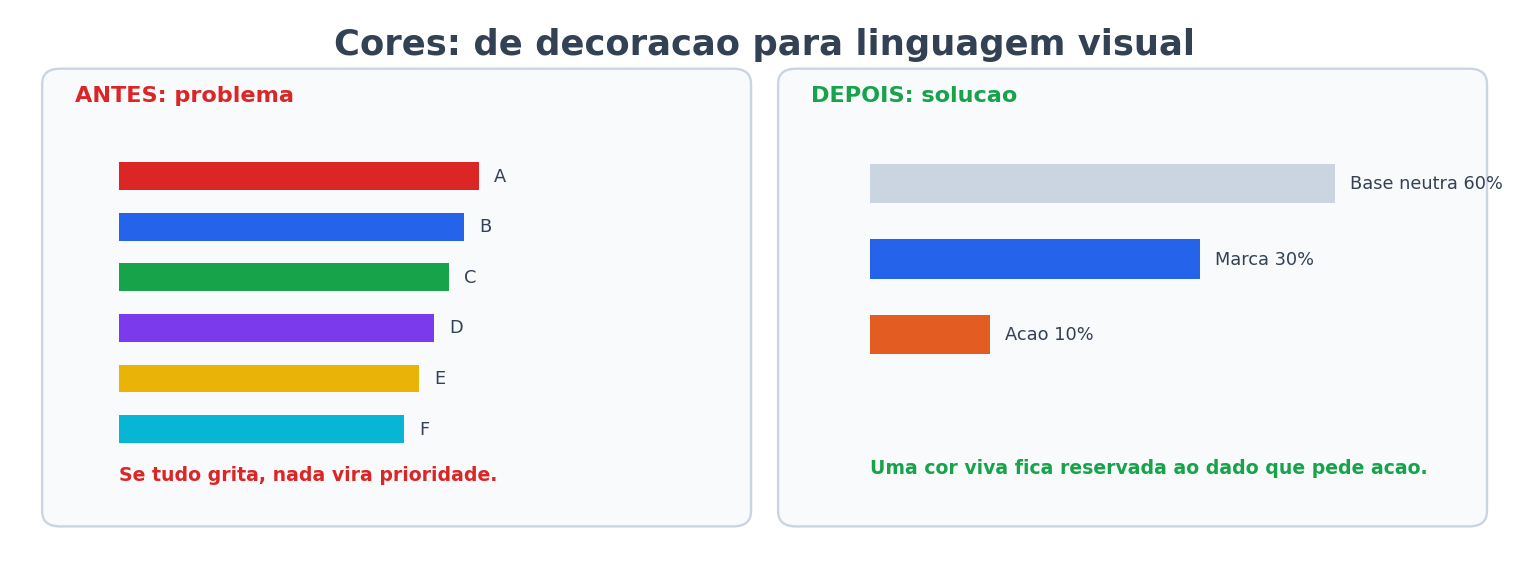
\includegraphics[width=0.58\textwidth]{semana_especial/outputs/cmp_cap1_cores.png}
\caption{Paleta de referência para dashboards. Cada cor tem uma função semântica única. Gráfico gerado pelo script \texttt{auto\_eda\_demo.py}.}
\end{figure}

\begin{BoardBox}[title=Paleta de 8 Funções --- Referência Rápida]
\begin{tabular}{@{}p{0.25cm}lll@{}}
\toprule
& \textbf{Hex} & \textbf{Função} & \textbf{Quando usar} \\
\midrule
\colorbox{colDestaque}{\phantom{M}} & \texttt{\#E35D22} & Destaque / ação urgente & O dado mais importante do dashboard \\
\colorbox{colPrimaria}{\phantom{M}} & \texttt{\#2563EB} & Primária / navegação    & Barras de base, links, filtros \\
\colorbox{colPositivo}{\phantom{M}} & \texttt{\#16A34A} & Positivo / meta atingida & Setas de alta, gaps positivos, badges OK \\
\colorbox{colAlerta}{\phantom{M}}   & \texttt{\#DC2626} & Alerta / falha / risco  & Abaixo da meta, KPI crítico \\
\colorbox{colAtencao}{\phantom{M}}  & \texttt{\#EAB308} & Atenção / monitorar     & Perto do limite, 80--99\% da meta \\
\colorbox{colNeutra}{\phantom{M}}   & \texttt{\#64748B} & Neutra / base           & Eixos, grades, texto secundário \\
\colorbox{colMarca}{\phantom{M}}    & \texttt{\#0B3D2E} & Marca / fundo escuro    & Header, rodapé, modo dark \\
\colorbox{colBgClaro}{\phantom{M}}  & \texttt{\#E2E8F0} & Background / fundo      & Área de trabalho do dashboard \\
\bottomrule
\end{tabular}
\end{BoardBox}

\paragraph{Acessibilidade e daltonismo.}
8\% dos homens e 0,5\% das mulheres têm alguma forma de daltonismo. O tipo mais comum é o deuteranopia (vermelho--verde). Regras práticas: (1) nunca use vermelho e verde como únicos diferenciadores --- adicione ícone de alta/baixa ou rótulo de texto; (2) use ferramentas como \textit{Color Oracle} ou \textit{Coblis} para simular; (3) o par azul--laranja tem alto contraste para daltonismo vermelho--verde e é a combinação padrão de grande parte dos dashboards corporativos.

\paragraph{Cor no Tableau e no QuickSight.}
No Tableau: \texttt{Format} $\to$ \texttt{Color} $\to$ \texttt{Edit Colors} define a paleta da view; use \texttt{Custom Diverging} para heatmaps; use \texttt{Single Color} com opacidade para barras onde o comprimento é o dado. No QuickSight: paletas são definidas no \textit{Theme JSON} e aplicadas globalmente no dataset; campos calculados com `ifelse` podem forçar cor semântica por condição.

% =============================================================
\section{Caminho do Olhar: Analista, Gerente e CEO}
\label{sec:olhar}
% =============================================================

Cada perfil de leitor olha para um dashboard em uma ordem diferente. Ignorar isso é o motivo pelo qual dashboards perfeitamente analíticos falham na sala de board. Entender o caminho do olhar de cada perfil é tão importante quanto escolher o gráfico certo.

\paragraph{O padrão F (analista).}
Pesquisas de eye-tracking de Jakob Nielsen (2006, \textit{Eyetracking Web Usability}) mostram que leitores técnicos percorrem o conteúdo em um padrão em forma de F: (1) leem a linha superior completa; (2) voltam ao início e leem a segunda linha; (3) varrem verticalmente o lado esquerdo em busca de palavras-chave. Implicação para dashboards: \textbf{coloque os dados mais importantes na primeira linha e no canto superior esquerdo}. O analista vai ler tudo, mas a ordem vai moldar o que ele interpreta como importante.

\paragraph{O padrão Z (executivo).}
O executivo com 5 minutos por dia varre o dashboard em Z: canto superior esquerdo $\to$ canto superior direito $\to$ diagonal $\to$ canto inferior esquerdo $\to$ canto inferior direito. Implicação: \textbf{Big Number + título-mensagem no topo esquerdo; Call to Action no rodapé direito; gráfico mais importante na diagonal}.

\begin{BoardBox}[title=Layout em Z para Dashboard Executivo]
\begin{verbatim}
[BIG NUMBER + Big Idea]  ->  [KPI2 | KPI3]
        diagonal
[Grafico diagnostico]    ->  [CALL TO ACTION]
\end{verbatim}
Percurso: (1) KPI principal com delta vs meta; (2) título-mensagem já conta a história;
(3) gráfico de diagnóstico para quem quer o detalhe; (4) CTA com verbo + prazo.
\end{BoardBox}

\begin{figure}[H]
\centering
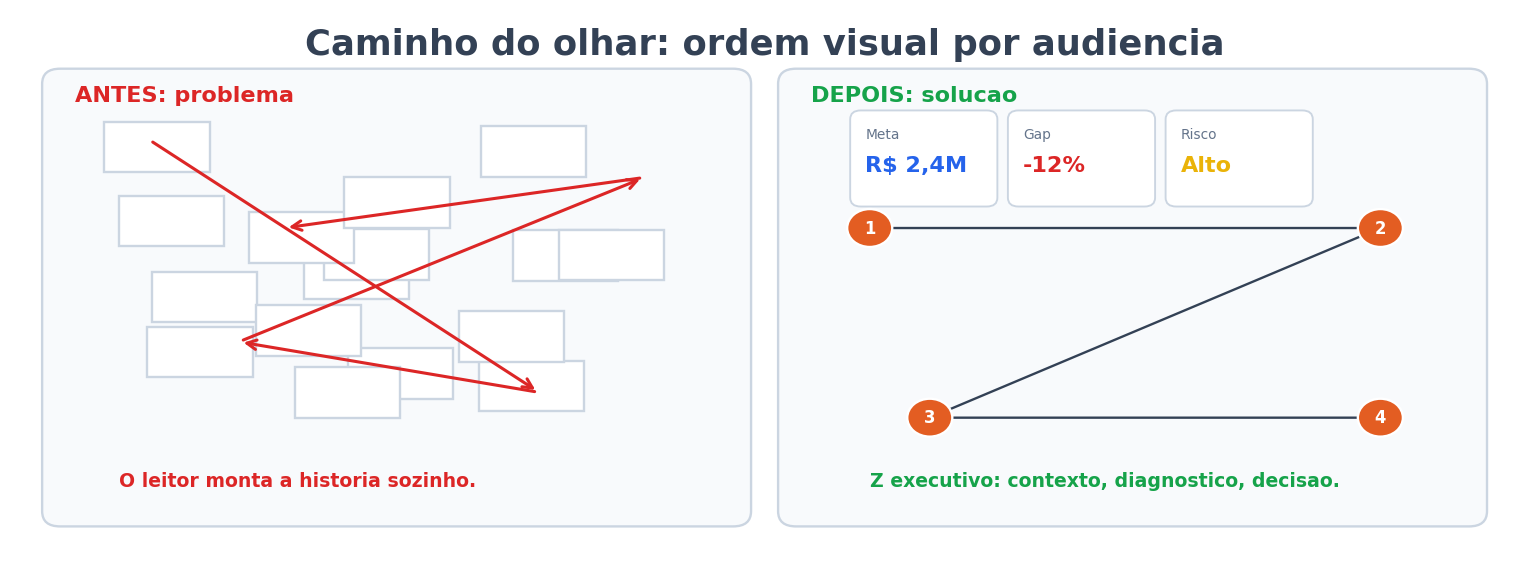
\includegraphics[width=0.58\textwidth]{semana_especial/outputs/cmp_cap1_olhar.png}
\caption{Caminho do olhar por perfil. Use esta figura em aula para mostrar que o mesmo dashboard pode falhar se a ordem visual não combinar com a audiência: o analista lê em F, o executivo varre em Z, e o gerente procura KPI, exceção e tabela de detalhe.}
\end{figure}

\paragraph{Perfil CEO: scanning semântico.}
O CEO não lê gráficos --- ele lê \emph{títulos}. Se os 4 títulos do dashboard entregam as mensagens, o CEO tomou a decisão antes de olhar qualquer eixo. A regra prática: todos os títulos de gráficos em linguagem de manchete de jornal. ``Gráfico de Barras'' $\to$ não. ``Sul lidera com 2,4$\times$ a média'' $\to$ sim.

\paragraph{Perfil gerente/gestor: diagonal + tabela.}
O gerente quer confirmar a hipótese que já tem. Ele vai direto ao gráfico que trata do seu KPI, verifica se o número confirma o que sente, e depois olha a tabela analítica no rodapé para entender as exceções. Implicação: \textbf{ofereça sempre uma tabela de detalhe no rodapé} --- ela não polui o design (ocupa a parte inferior que o executivo ignora) mas salva o gerente de tomar uma decisão com dado incompleto.

\paragraph{Perfil analista: leitura completa em espiral.}
O analista começa no Big Number, vai para o scatter, tenta reproduzir o cálculo, encontra a nota metodológica, cruza com a tabela, e só então forma uma opinião. Para esse perfil, inclua: (1) definição de todas as métricas em tooltip ou nota de rodapé; (2) período de referência explícito; (3) fonte dos dados.

% =============================================================
\section{Carga Cognitiva e Dashboard Cognitivo}
\label{sec:cognitivo}
% =============================================================

A \textbf{teoria da carga cognitiva} (Sweller, 1988) distingue três tipos de carga mental que afetam a absorção de informação. Entender isso explica por que dashboards muito elaborados technicamente falham na comunicação.

\begin{BoardBox}[title=Os 3 Tipos de Carga Cognitiva]
\begin{enumerate}
  \item \textbf{Carga intrínseca:} complexidade inerente ao conteúdo (o dado em si é complicado? a análise exige raciocínio?). Você não pode reduzir isso sem simplificar a análise.
  \item \textbf{Carga extrínseca (extraneous):} esforço causado pelo design ruim. Legenda separada que exige desvio do olhar; cores sem propósito que forçam decodificação; texto e gráfico contradizendo-se. Isso é \textbf{eliminável} com bom design.
  \item \textbf{Carga germane (útil):} esforço que forma aprendizado e schema mental. É o que sobra quando você elimina a carga extrínseca. Você quer maximizar isso.
\end{enumerate}
\smallskip
\textbf{Objetivo do bom design:} eliminar toda a carga extrínseca para liberar capacidade cognitiva para a carga útil.
\end{BoardBox}

\paragraph{Princípios de Gestalt aplicados a dashboards.}
A psicologia da Gestalt descreve como o cérebro organiza elementos visuais em padrões. Cinco princípios diretos:

\begin{BoardBox}[title=Gestalt em Dashboards]
\begin{tabular}{@{}lp{4.2cm}p{5.8cm}@{}}
\toprule
\textbf{Princípio} & \textbf{O que significa} & \textbf{Aplicação prática} \\
\midrule
Proximidade   & Elementos próximos parecem relacionados  & KPIs do mesmo tema agrupados com espaço em branco entre grupos \\
Similaridade  & Elementos parecidos parecem relacionados & Mesma cor = mesma categoria; mesmo formato = mesma hierarquia \\
Fechamento    & O cérebro completa formas incompletas    & Enclosure (caixa) ao redor de KPIs = grupo implícito sem linha pesada \\
Continuidade  & O olho segue linhas e padrões de fluxo  & Gráfico de linhas sugere tendência; use linhas de referência \\
Figura-fundo  & Um elemento se destaca, o resto recua   & 1 cor de destaque em fundo cinza é pura figura-fundo \\
\bottomrule
\end{tabular}
\end{BoardBox}

\paragraph{Dashboard cognitivo: definição.}
Um dashboard cognitivo (termo popularizado por Stephen Few em \textit{Show Me the Numbers}, 2012) é aquele que foi projetado para \emph{minimizar a carga extrínseca e maximizar a carga germane}: título-mensagem que já entrega o insight; cor de destaque que guia o olho; hierarquia visual clara (importante grande, secundário pequeno); remoção de todo chartjunk; e estrutura narrativa que replica o processo de decisão da audiência-alvo.

\begin{figure}[H]
\centering
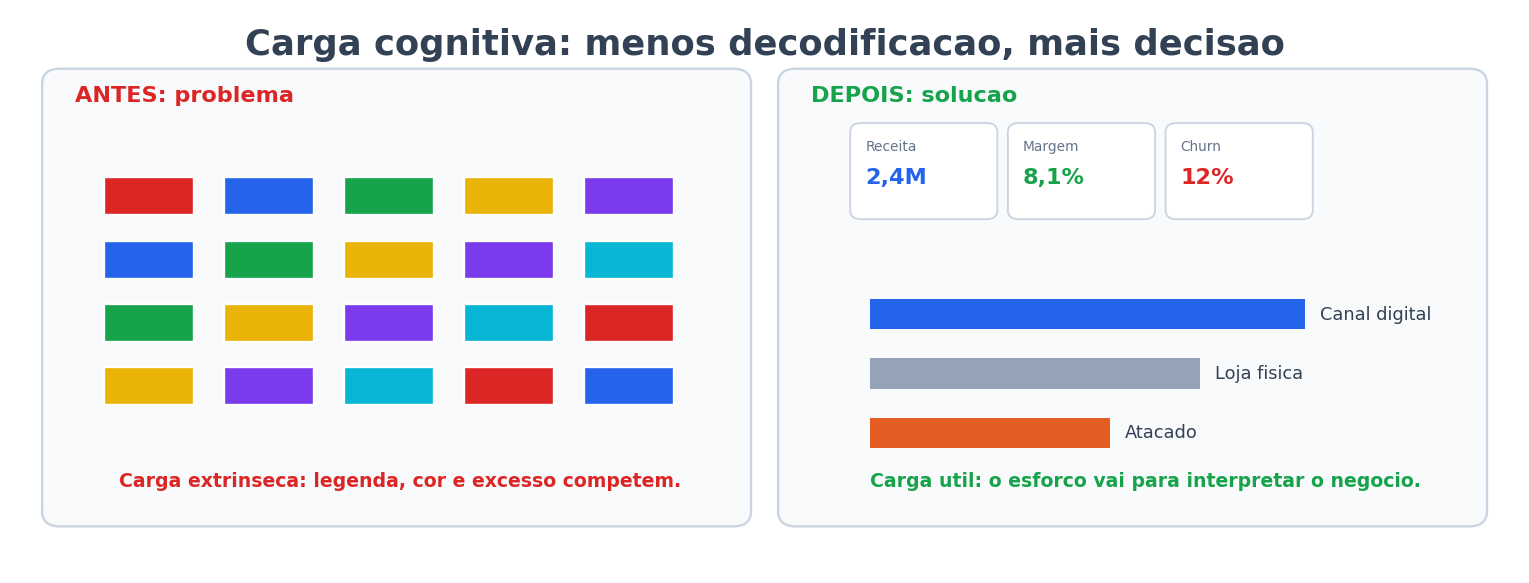
\includegraphics[width=0.58\textwidth]{semana_especial/outputs/cmp_cap1_carga.png}
\caption{Carga cognitiva aplicada a dashboards. À esquerda, o leitor gasta energia decodificando cores, formas e excesso de gráficos; à direita, a energia mental é transferida para entender o problema e decidir.}
\end{figure}

\paragraph{Número mágico 7 ± 2.}
George Miller (1956) demonstrou que a memória de trabalho humana processa 7 (mais ou menos 2) objetos simultâneos. Para dashboards: máximo de 7 KPIs na tela inicial; máximo de 7 categorias por gráfico (agrupe o restante em ``Outros''); máximo de 7 cores distintas numa paleta. Acima desses limites, a interpretação falha mesmo com dados corretos.

% =============================================================
\section{Insights Informativos}
\label{sec:insight_info}
% =============================================================

Um insight informativo é uma observação extraída dos dados que \textbf{aumenta o entendimento} de uma situação mas \emph{não orienta uma ação específica e imediata}. Ele tem valor: reduz incerteza, confirma hipóteses, fornece contexto. O problema começa quando o analista entrega \emph{apenas} insights informativos numa reunião executiva --- porque executivos não precisam de mais informação, precisam de mais clareza sobre o que fazer.

\begin{BoardBox}[title=Características de um Insight Informativo]
\begin{enumerate}
  \item \textbf{Descreve um padrão real:} algo que estava oculto nos dados e que a audiência não sabia.
  \item \textbf{É factual e verificável:} pode ser reproduzido com os mesmos dados.
  \item \textbf{Não tem urgência intrínseca:} ``interessante, mas e daí?'' é a reação esperada.
  \item \textbf{Serve de base para insights acionáveis:} todo bom insight acionável parte de um informativo.
\end{enumerate}
\end{BoardBox}

\textbf{Exemplos de insights informativos:}

\begin{itemize}
  \item ``A distribuição de Exam\_Score é aproximadamente normal (média 67,2; DP 3,9), o que indica que o dataset não tem viés de seleção severo.''
  \item ``Frequência (Attendance) tem a maior correlação com a nota final ($r = 0{,}58$), acima de horas de estudo ($r = 0{,}45$).''
  \item ``Clientes do segmento Premium têm ticket médio 3,2$\times$ maior que o segmento Standard.''
  \item ``O churn em janeiro de 2025 foi 12\% --- o maior dos últimos 24 meses.''
\end{itemize}

Insights informativos são valiosos em relatórios de EDA, em apresentações para times técnicos e em bases de conhecimento internas. O erro é confundi-los com o produto final de uma análise para a diretoria.

\begin{figure}[H]
\centering
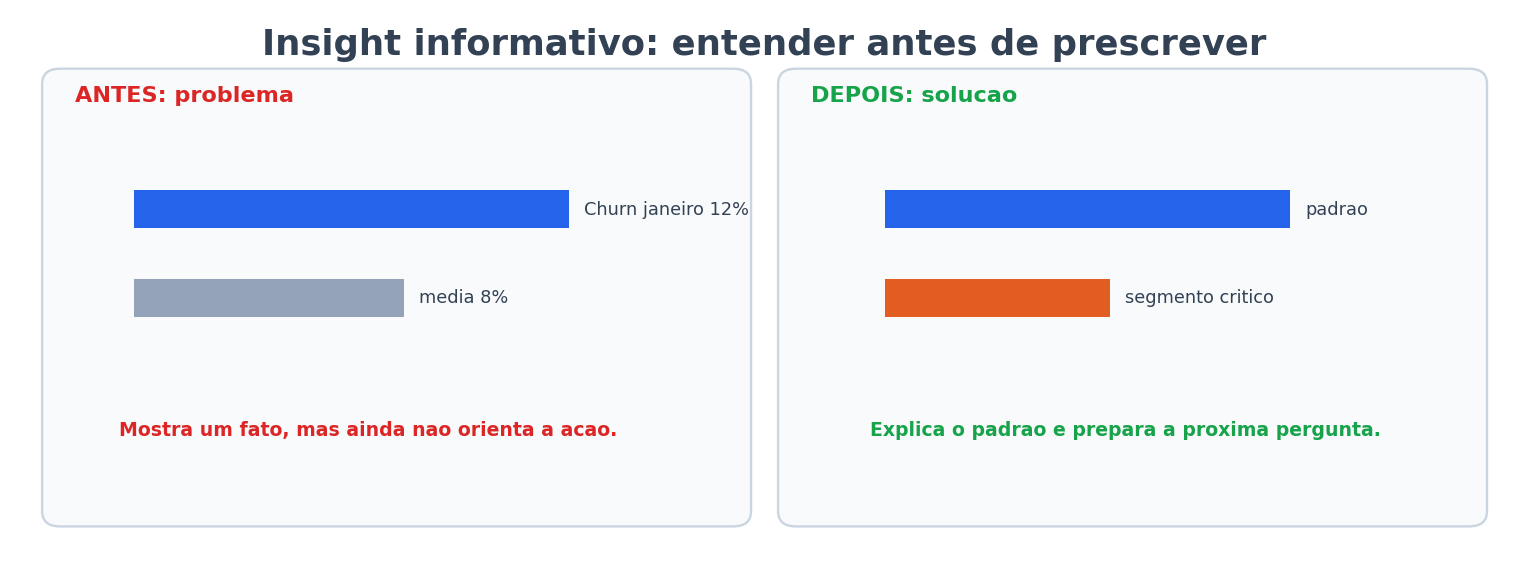
\includegraphics[width=0.58\textwidth]{semana_especial/outputs/cmp_cap1_insight_info.png}
\caption{Insight informativo em dashboard. Ele melhora o entendimento, mas ainda deixa perguntas executivas em aberto: gravidade, responsável, ação e impacto.}
\end{figure}

% =============================================================
\section{Insights Acionáveis: Do Dado à Decisão}
\label{sec:insight_acion}
% =============================================================

Este é o tópico central de qualquer analista que trabalha para a tomada de decisão. Um insight acionável \textbf{prescreve uma ação específica, direcionada a um responsável, com estimativa de impacto e prazo}. Ele não descreve o passado --- ele orienta o futuro. A diferença entre analistas júnior e sênior, na prática bancária e em qualquer grande corporação, é exatamente a capacidade de transformar observações numéricas em recomendações que mudam o comportamento de alguém.

\begin{BoardBox}[title=Fórmula do Insight Acionável --- 5 Componentes]
\begin{enumerate}
  \item \textbf{Observação:} padrão não-óbvio extraído dos dados.
  \item \textbf{Evidência:} o dado que sustenta a observação (com magnitude e significância).
  \item \textbf{Causa raiz (quando possível):} por que isso está acontecendo?
  \item \textbf{Ação prescrita:} verbo + objeto + quantidade + canal.
  \item \textbf{Impacto estimado:} resultado esperado em métrica de negócio + prazo.
\end{enumerate}
\smallskip
\textbf{Template:} ``[Observação] porque [evidência]. Se [ação prescrita] então [impacto estimado] em [prazo], responsável: [stakeholder].''
\end{BoardBox}

\paragraph{Por que a maioria dos analistas não consegue fazer isso.}
O bloqueio é conceitual: o analista foi treinado para \emph{descrever} dados, não para \emph{prescrever} ações. Descrever é seguro --- ninguém erra ao reportar que ``as vendas caíram 8\%''. Prescrever exige entender o negócio, assumir uma hipótese causal e aceitar que pode estar errado. O sênior aceita esse risco porque o valor gerado pela ação certa supera muito o custo de estar errado em uma recomendação específica.

\paragraph{Exemplos completos --- 8 domínios.}

Os exemplos a seguir seguem a estrutura de 5 componentes. Leia devagar: a diferença entre o insight informativo (coluna ``sem ação'') e o acionável (coluna ``com ação'') é a diferença de impacto na carreira de um analista.

\medskip
\textbf{Exemplo 1 --- Banco: análise de churn de cartão de crédito}

\textit{Informativo:} ``Clientes com menos de 20 transações por ano têm taxa de churn de 38\%, vs 6\% para clientes com mais de 50 transações.''

\textit{Acionável:} ``Clientes com frequência de uso $<$ 20 trans/ano e saldo médio $<$ R\$2k têm 38\% de probabilidade de cancelamento --- 3,4 pp acima da base. Acionar campanha de reengajamento personalizado via app (cashback + limite temporário) para os 8.200 clientes nesse perfil pode reverter 30\% do churn projetado, preservando R\$1,4M em receita de juros e anuidade nos próximos 12 meses. Responsável: Gerência de CRM. Prazo de implementação: 3 semanas.''

\medskip
\textbf{Exemplo 2 --- Varejo: pricing de produto}

\textit{Informativo:} ``Produtos com desconto $>$ 20\% têm margem média de $-4\%$.''

\textit{Acionável:} ``Descontos acima de 20\% em Linha Branca na Região Sul destroem R\$120k de margem por trimestre sem aumentar o volume de unidades (elasticidade próxima de zero na análise de regressão). Capear o desconto máximo em 12\% mantém a competitividade de preço percebida e projeta recuperação de R\$85k de margem trimestral. Responsável: Gerência Comercial Sul. Prazo: implementar na campanha de inverno (início de julho).''

\medskip
\textbf{Exemplo 3 --- RH: turnover de TI}

\textit{Informativo:} ``O departamento de TI tem turnover de 28\%, acima da média corporativa de 12\%.''

\textit{Acionável:} ``Engenheiros de TI com menos de 2 anos de empresa e sem promoção nos últimos 36 meses têm 3$\times$ mais probabilidade de saída que a média (28\% vs 9\%). Esse perfil representa 41 funcionários. Implantar programa de mentoria acelerada + revisão de faixa salarial para esse grupo específico pode reduzir o turnover de 28\% para 15\%, economizando R\$270k/ano em custo de reposição (R\$18k/funcionário $\times$ 15 saídas evitadas). Responsável: HRBP de TI + Diretor de Engenharia. Prazo: começar em 30 dias para impactar a janela de avaliação semestral.''

\medskip
\textbf{Exemplo 4 --- Saúde: readmissão hospitalar}

\textit{Informativo:} ``Pacientes com diabetes + hipertensão têm taxa de readmissão em 30 dias de 34\%.''

\textit{Acionável:} ``Pacientes diabéticos com HbA1c $>$ 9 e diagnóstico de HAS que receberam alta sem consulta de retorno agendada têm 34\% de readmissão em 30 dias vs 8\% quando o retorno está agendado. Implementar protocolo de agendamento obrigatório na alta para os 1.200 pacientes nesse perfil anual pode evitar 312 readmissões, economizando R\$3,7M (R\$12k/internação), além de melhorar o indicador de qualidade AHRQ-PSI. Responsável: Gerência de Assistência. Prazo: protocolo ativo no próximo semestre.''

\medskip
\textbf{Exemplo 5 --- E-commerce: logística}

\textit{Informativo:} ``O estado do Amazonas tem atraso médio de 4,7 dias acima da estimativa.''

\textit{Acionável:} ``Pedidos de Eletrônicos em AM com prazo estimado $<$ 7 dias chegam em média 4,7 dias atrasados, gerando review médio de 2,8 estrelas e taxa de devolução 18\% acima da média. Substituir a transportadora atual por operador regional com SLA de 5 dias para essa rota reduz o atraso estimado em 70\%, projeta melhora do review para 4,1 estrelas e reduz devoluções em R\$95k/semestre. Responsável: Gerência de Logística. Prazo: RFP para transportadora em 45 dias.''

\medskip
\textbf{Exemplo 6 --- Fintech: crédito}

\textit{Informativo:} ``A inadimplência de empréstimo pessoal cresceu 3 pp em Q1/2026.''

\textit{Acionável:} ``Clientes de empréstimo pessoal com renda variável (profissional autônomo) que acessaram o produto em fevereiro/março têm inadimplência de 19\%, contra 7\% para clientes com renda fixa. O crescimento de 3 pp na inadimplência total é explicado em 78\% por esse segmento (análise de decomposição). Ajustar a política de crédito para limitar o LTV de empréstimo pessoal a 60\% da renda variável comprovada pode reduzir a inadimplência desse perfil de 19\% para 10\%, preservando R\$4,2M em provisão de crédito no próximo trimestre. Responsável: Gerência de Risco de Crédito. Prazo: vigência imediata para novas contratações.''

\medskip
\textbf{Exemplo 7 --- Educação (dataset StudentPerformance)}

\textit{Informativo:} ``Frequência (Attendance) tem correlação de 0,58 com Exam\_Score, sendo o preditor mais forte entre as variáveis numéricas.''

\textit{Acionável:} ``Alunos com frequência $<$ 75\% nos meses de março--abril têm nota final média 9,3 pts abaixo da média geral (67,2), e 34\% deles reprovam. Implementar sistema de alerta automático por WhatsApp para responsáveis quando o aluno atingir 3 faltas consecutivas pode recuperar 40\% desses alunos (baseado em piloto de 2024), reduzindo a taxa de reprovação de 8\% para 4,8\%, equivalendo a 216 alunos aprovados adicionais por semestre. Responsável: Coordenação Pedagógica + TI. Prazo: sistema ativo no início do semestre seguinte.''

\medskip
\textbf{Exemplo 8 --- Marketing digital: aquisição}

\textit{Informativo:} ``O CAC médio pelo canal Google Ads é R\$48, contra R\$31 pelo canal Organic.''

\textit{Acionável:} ``O canal Google Ads tem CAC 55\% maior que o orgânico, mas o LTV dos clientes adquiridos por Google Ads é apenas 8\% maior (R\$320 vs R\$296). O ROI ajustado ao LTV do canal pago é negativo ($-$4\%) no primeiro ano. Redirecionar 40\% do orçamento de Google Ads para SEO/Content durante 6 meses projeta redução do CAC médio de R\$48 para R\$35, com impacto de $-$12\% no volume de aquisição no curto prazo mas retorno positivo a partir do mês 8. Responsável: Gerência de Marketing. Prazo: próximo ciclo de orçamento (Q3 2026).''

\paragraph{Como treinar a habilidade de gerar insights acionáveis.}
O caminho mais rápido é forçar a pergunta ``\emph{e daí?}'' sobre cada dado encontrado. Toda vez que você escrever uma observação, pergunte: ``E daí?'' até chegar num verbo de ação ligado a um responsável. Veja a cadeia:

\begin{BoardBox}[title=A Cadeia ``E Daí?'' --- Exercício Prático]
\textbf{Observação inicial:} ``O churn subiu 3\%.'' \quad \textbf{E daí?}\\
\textbf{Nível 2:} ``Clientes do segmento X estão cancelando mais.'' \quad \textbf{E daí?}\\
\textbf{Nível 3:} ``Clientes do segmento X com produto Y cancelam 4$\times$ mais no 3$^\circ$ mês.'' \quad \textbf{E daí?}\\
\textbf{Nível 4:} ``O problema é que o onboarding do produto Y não é completado por 60\% dos clientes.'' \quad \textbf{E daí?}\\
\textbf{Insight acionável:} ``Criar fluxo de onboarding guiado no app para produto Y, com nudge no dia 15, pode reduzir o churn do segmento X de 18\% para 8\%, preservando R\$XX em ARR. Responsável: PM + CRM. Prazo: 4 semanas.''
\end{BoardBox}

\begin{figure}[H]
\centering
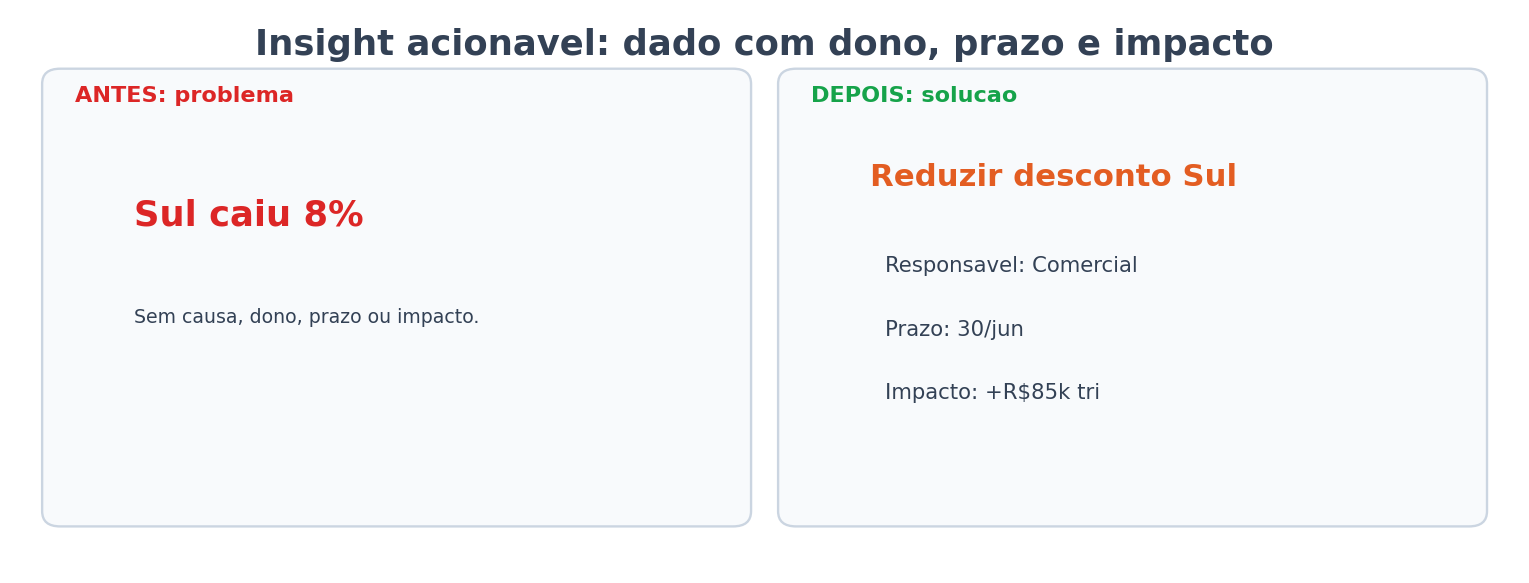
\includegraphics[width=0.58\textwidth]{semana_especial/outputs/cmp_cap1_insight_acionavel.png}
\caption{Dashboard sem ação versus dashboard com insight acionável. O segundo não apenas descreve o problema: ele explicita o que fazer, quem deve fazer, até quando e qual impacto esperado.}
\end{figure}

% =============================================================
\section{Dashboard as Code: AWS e QuickSight}
\label{sec:daac}
% =============================================================

\textbf{Dashboard as Code (DaC)} é a prática de definir, versionar e publicar dashboards inteiramente via código e infraestrutura como código (IaC), eliminando configuração manual via interface gráfica. Os benefícios diretos para um time de analytics bancário são: rastreabilidade via Git, reprodutibilidade entre ambientes (dev/homol/prod), revisão de mudanças por Pull Request, e orquestração programática de dezenas de dashboards.

\paragraph{AWS QuickSight e as APIs de criação.}
O QuickSight expõe uma API REST completa (\textit{aws quicksight} via Boto3 ou CLI) que permite criar e atualizar todos os recursos: datasets, análises, dashboards e permissões. Os objetos principais na hierarquia são:

\begin{BoardBox}[title=Hierarquia de Objetos no QuickSight]
\begin{tabular}{@{}llp{6.5cm}@{}}
\toprule
\textbf{Objeto} & \textbf{API} & \textbf{Descrição} \\
\midrule
DataSource    & \texttt{create-data-source}    & Conexão ao S3/Redshift/Athena/RDS \\
DataSet       & \texttt{create-data-set}       & Schema, joins, campos calculados, filtros de linha \\
Analysis      & \texttt{create-analysis}       & Canvas de edição (não publicado) \\
Dashboard     & \texttt{create-dashboard}      & Versão publicada de uma Analysis \\
Template      & \texttt{create-template}       & Snapshot de uma Analysis reutilizável cross-account \\
Theme         & \texttt{create-theme}          & Paleta de cores, fontes e layout globais \\
\bottomrule
\end{tabular}
\end{BoardBox}

\paragraph{Fluxo conceitual do Dashboard as Code.}
Para esta aula, o importante não é decorar código de Boto3 ou CDK. O ponto central é entender que o dashboard deixa de ser uma peça manual feita no clique e passa a ser um artefato governado: nasce de uma regra de negócio, é versionado, revisado, homologado e publicado com rastreabilidade.

\begin{figure}[H]
\centering
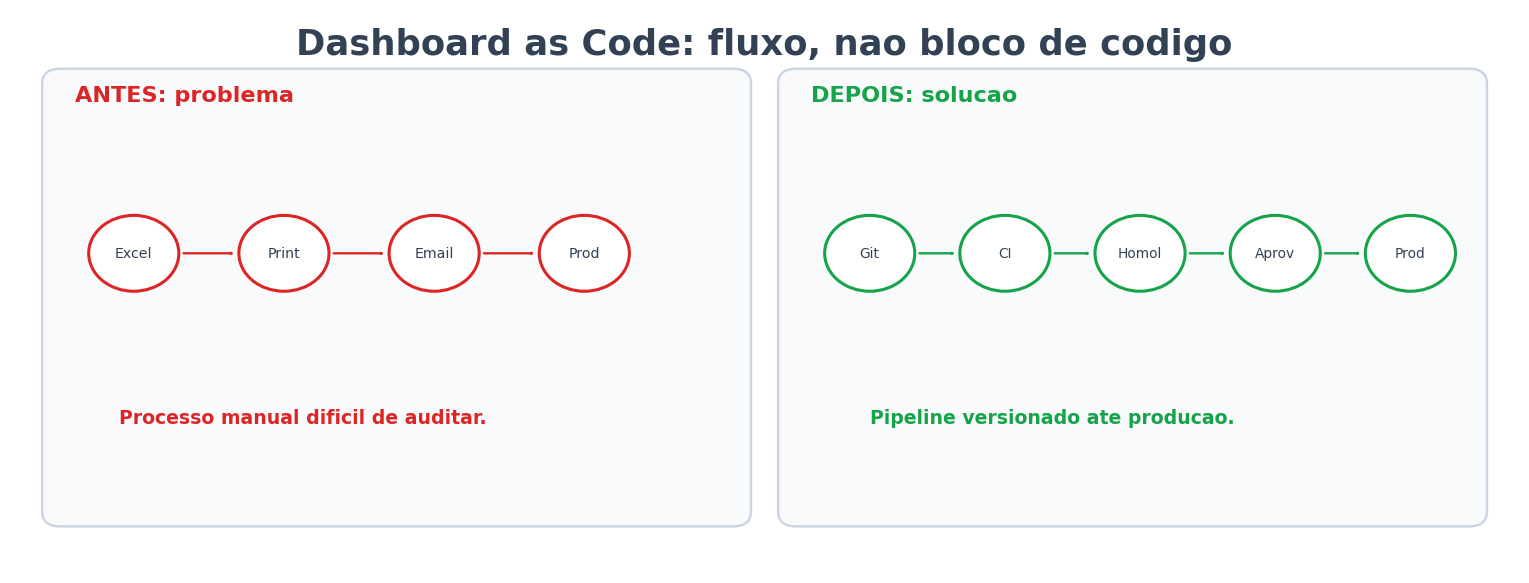
\includegraphics[width=0.58\textwidth]{semana_especial/outputs/cmp_cap1_dac.png}
\caption{Fluxo conceitual de Dashboard as Code. A criação programática só faz sentido quando protege governança: regra de negócio clara, definição versionada, revisão por pares, homologação e publicação controlada.}
\end{figure}

\paragraph{Fluxo de trabalho DaC com Git.}
O padrão recomendado para times de analytics em bancos: (1) \texttt{feature/dashboard-churn} branch; (2) código Python com definição de datasets + análise em JSON (exportado via \texttt{describe-analysis-definition}); (3) PR com revisão de outro analista; (4) merge em \texttt{main} dispara GitHub Actions que chama \texttt{boto3.update\_dashboard}; (5) tags de versão correspondem a versões do QuickSight.

\paragraph{Asset Bundle Export/Import.}
Para migração entre contas (dev $\to$ prod) sem recriar tudo manualmente, o QuickSight oferece desde 2023 o \textbf{Asset Bundle} API: exporta análises, dashboards, datasets e temas em JSON e importa em outra conta com substituição de ARNs. Isso é o equivalente ao \texttt{terraform plan/apply} para dashboards.

% =============================================================
\section{AED Automática: Bibliotecas, Relatórios e Interpretação}
\label{sec:autoeda}
% =============================================================

As bibliotecas de AED automática (profiling) fazem em uma linha o que levaria horas de código manual: calculam estatísticas descritivas, detectam outliers, mapeiam correlações, identificam dados ausentes, avaliam distribuições e geram relatório HTML completo. Elas não substituem a análise --- substituem a parte mecânica para que o analista foque na interpretação.

\begin{BoardBox}[title=Principais Bibliotecas de AED Automática (Python)]
\begin{tabular}{@{}lp{3.5cm}p{5.8cm}@{}}
\toprule
\textbf{Biblioteca} & \textbf{Melhor para} & \textbf{Diferencial} \\
\midrule
\texttt{ydata-profiling} & Relatório completo solo & 1 linha; HTML interativo; detecta correlações, outliers, duplicatas, alertas de qualidade \\
\texttt{sweetviz}        & Comparação de grupos    & Visualiza diferenças entre treino/teste ou segmentos lado a lado; target analysis \\
\texttt{autoviz}         & Visualizações rápidas   & Gera gráficos automaticamente sem HTML; bom para exploração rápida \\
\texttt{D-Tale}          & Exploração interativa   & Interface web local tipo Excel interativo; edição de dados em tempo real \\
\texttt{lux}             & Recomendação automática & Sugere visuais relevantes contextualizados ao DataFrame; integra Jupyter \\
\bottomrule
\end{tabular}
\end{BoardBox}

\paragraph{Como ler um relatório automático.}
Nesta aula, não precisamos decorar comandos. O que importa é saber interpretar o HTML produzido por essas ferramentas. Primeiro olhe os \textbf{alertas de qualidade}: dados ausentes, duplicatas, cardinalidade alta e colunas constantes. Depois leia as \textbf{distribuições}: assimetria, outliers e concentração. Em seguida, veja \textbf{correlações e associações}: elas sugerem hipóteses, mas não provam causalidade. Por fim, transforme o relatório em perguntas de negócio: ``qual variável explica o resultado?'', ``qual grupo merece intervenção?'', ``que dado precisa ser validado antes da decisão?''.

\begin{figure}[H]
\centering
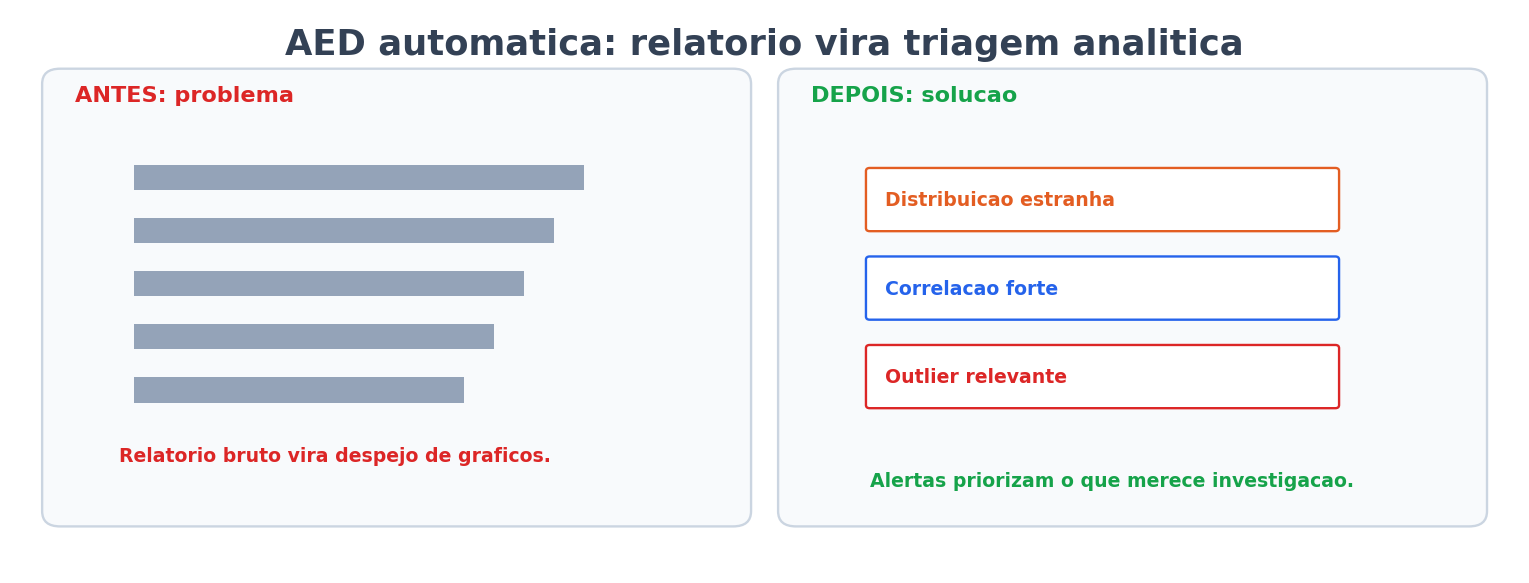
\includegraphics[width=0.58\textwidth]{semana_especial/outputs/cmp_cap1_autoeda.png}
\caption{Fluxo de leitura da AED automática. O HTML é um ponto de partida: ele encontra sinais, mas o analista precisa explicar o significado e formular a próxima pergunta.}
\end{figure}

\paragraph{Exemplo real: StudentPerformanceFactors.csv.}

Rodamos \texttt{ydata-profiling} (modo minimal, 6607 registros, 20 variáveis) e \texttt{sweetviz} no dataset deste curso. Os relatórios HTML estão em \texttt{semana\_especial/outputs/}:
\begin{itemize}
  \item \texttt{ydata\_profiling\_report.html} --- perfil completo com alertas de qualidade, correlações, distribuições
  \item \texttt{sweetviz\_report.html} --- target analysis com Exam\_Score como variável alvo
\end{itemize}

Em aula, use esses relatórios como material de inspeção: eles mostram distribuições, correlações, scatterplots e variáveis categóricas. O PDF mantém apenas o comparativo acima para não repetir quatro figuras exploratórias onde uma síntese visual resolve melhor.

\paragraph{Alertas automáticos que o ydata-profiling detecta.}
O relatório HTML sinaliza automaticamente: variáveis com $>$ 5\% de dados ausentes; colunas com alta correlação ($>$ 0,9) que indicam redundância; variáveis com cardinalidade muito alta (suspeita de ID); distribuições muito assimétricas (candidatas a transformação log); valores constantes ou quase-constantes.

\paragraph{Quando NÃO usar AED automática.}
Quando o dataset tem $>$ 10M de linhas (o relatório trava ou demora demais --- use uma amostra estratificada de 50k--100k linhas); quando as variáveis têm semântica muito específica do negócio que a biblioteca não conhece (ex.: códigos de agência bancária precisam de dicionário manual); quando o objetivo já é confirmatory (você já sabe o que procura --- vá direto).

% =============================================================
\section{Arquitetura de Agentes para AED e Dashboards}
\label{sec:agentes}
% =============================================================

A abordagem de agentes para análise de dados está passando de experimento acadêmico para realidade em grandes bancos e fintechs em 2025--2026. A ideia central é substituir o fluxo manual linear (analista faz EDA $\to$ analista faz perguntas $\to$ analista constrói dashboard) por um \textbf{pipeline orquestrado de agentes especializados}, cada um responsável por uma etapa e passando seu output como contexto estruturado para o próximo.

\paragraph{A arquitetura descrita.}
O pipeline que estamos construindo no banco tem a seguinte cadeia:

\begin{BoardBox}[title=Pipeline Multi-Agente --- Etapas]
\begin{enumerate}
  \item \textbf{Agente Discovery:} lê o contrato de negócio (dores, KPIs, audiência), carrega o dataset, calcula estatísticas descritivas, mapeia correlações, detecta outliers. Output: JSON com contexto estruturado.
  \item \textbf{Agente de Insights:} recebe o JSON do Agente 1, consulta a base especializada de insights (seção 9), e gera insights acionáveis candidatos com score de relevância.
  \item \textbf{Agente de Storyboard:} define Big Idea, estrutura 3 zonas (Contexto/Diagnóstico/Recomendação), monta a sequência de gráficos e os títulos-mensagem.
  \item \textbf{Agente Protótipo:} gera HTML completo do dashboard com Chart.js, auto-contido, com dados reais do dataset. Output: \texttt{prototipo.html}.
  \item \textbf{Agente de Infraestrutura (AWS):} recebe o protótipo aprovado, converte para definição QuickSight (JSON/API), cria DataSet + Analysis + Dashboard via Boto3.
  \item \textbf{Agente de Documentação:} gera changelog, dicionário de métricas e runbook automaticamente a partir dos metadados dos agentes anteriores.
\end{enumerate}
\smallskip
\textbf{Orquestrador:} LangChain / LangGraph / AWS Step Functions (para pipelines produtivos em nuvem).
\end{BoardBox}

\begin{figure}[H]
\centering
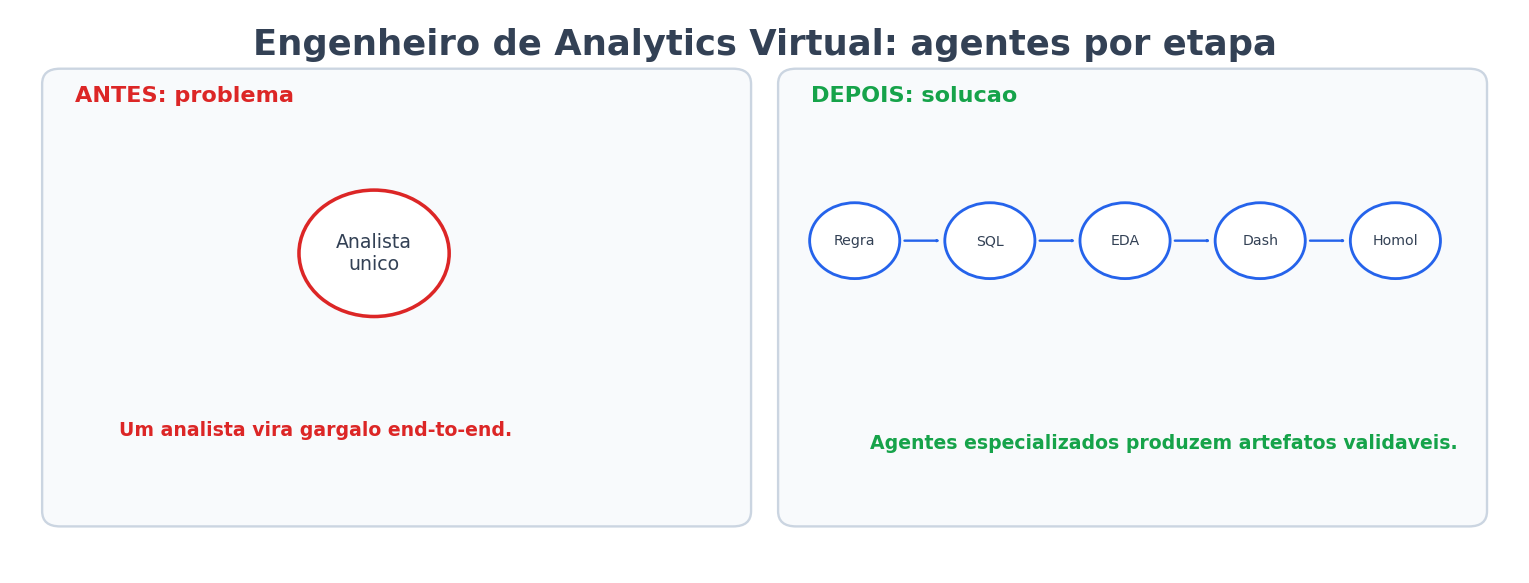
\includegraphics[width=0.58\textwidth]{semana_especial/outputs/cmp_cap1_agentes.png}
\caption{Arquitetura lúdica do Engenheiro de Analytics Virtual. A ideia prática é end-to-end: da regra de negócio até a publicação do dashboard, cada agente produz um artefato que pode ser revisado e homologado.}
\end{figure}

\paragraph{Protótipo gerado pelo pipeline.}

O script \texttt{agente\_prototipo\_html.py} executa os Agentes 1--4 localmente, sem LLM externo, usando apenas pandas e Chart.js. O arquivo \texttt{prototipo\_dashboard\_agente.html} está em \texttt{semana\_especial/outputs/}. Ele demonstra a estrutura que o pipeline mais completo (com LLM) produziria.

\paragraph{Como funcionaria na prática.}
Imagine que a área de negócio pede: ``o churn do cartão Premium subiu e precisamos decidir uma campanha''. O Agente de Negócio transforma isso em contrato: audiência, dor, métrica-alvo, restrições e prazo. O Agente de Dados valida tabelas, chaves, granularidade e qualidade. O Agente SQL cria ou sugere views analíticas. O Agente EDA procura padrões. O Agente de Insights transforma padrões em recomendações. O Agente Storyboard escolhe a sequência narrativa. O Agente Protótipo gera um HTML para homologação rápida. Só depois de aprovado entram os agentes de produção: criação de dataset, dashboard no BI, permissões, documentação e changelog.

\begin{BoardBox}[title=Artefatos por Agente]
\begin{tabular}{@{}lp{8.7cm}@{}}
\toprule
\textbf{Agente} & \textbf{Artefato entregue} \\
\midrule
Negócio & contrato de análise: dor, KPI, audiência, decisão esperada \\
Dados/SQL & tabela, view ou consulta validada com dicionário de métricas \\
EDA & resumo visual de padrões, outliers, correlações e alertas \\
Insights & 2--3 recomendações acionáveis com impacto e responsável \\
Storyboard & Big Idea, zonas do dashboard e títulos-mensagem \\
Protótipo & HTML navegável para homologação com usuário \\
Produção & dashboard publicado, permissões, documentação e versão \\
\bottomrule
\end{tabular}
\end{BoardBox}

\paragraph{Padrões de multi-agente: ReAct, Chain-of-Thought e Tool-Use.}
Três padrões são relevantes para o pipeline de analytics: (1) \textbf{ReAct} (Yao et al., 2022) --- o agente raciocina (\textit{Thought}) e então age (\textit{Action}), iterando até atingir o objetivo; ideal para o Agente de Insights que precisa testar hipóteses. (2) \textbf{Chain-of-Thought} (Wei et al., 2022) --- o agente externaliza o raciocínio passo a passo antes de entregar o output; útil no Agente de Storyboard para justificar cada decisão de layout. (3) \textbf{Tool-Use / Function-Calling} (OpenAI, 2023) --- o agente chama funções externas (Boto3, Tableau API, base de dados) de forma estruturada; é o que habilita o Agente de Infraestrutura a criar dashboards reais no QuickSight.

% =============================================================
\section{Como Criar Insights Acionáveis: Base Especializada}
\label{sec:insight_base}
% =============================================================

O maior gargalo para gerar insights acionáveis em escala (em um time de 20 analistas, para dezenas de produtos) é a \textbf{inconsistência de qualidade}. Cada analista usa sua própria definição do que é um insight, seu próprio template, sua própria escala de urgência. O resultado: 80\% dos ``insights'' entregues são observações descritivas, e os executivos param de ler relatórios de dados.

A solução é criar uma \textbf{base especializada em insights}: um repositório estruturado (tabela, vector store ou knowledge base) que contém exemplos de alta qualidade validados pelo negócio, que serve de referência para analistas humanos e de few-shot context para agentes de IA.

\begin{figure}[H]
\centering
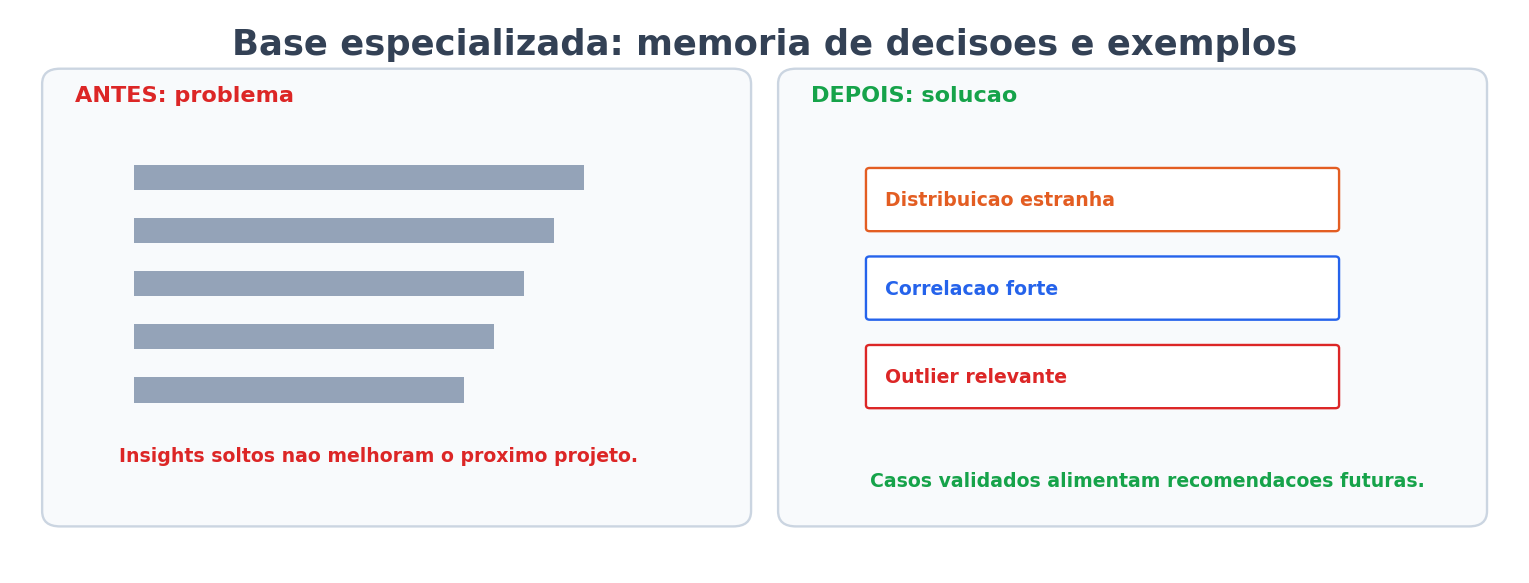
\includegraphics[width=0.58\textwidth]{semana_especial/outputs/cmp_cap1_base_insights.png}
\caption{Base especializada de insights. Ela funciona como memória de qualidade: exemplos validados alimentam novos agentes e padronizam o que a turma deve chamar de insight acionável.}
\end{figure}

\begin{BoardBox}[title=Tabela \texttt{insight\_base}]
\small
\begin{tabular}{@{}p{3.2cm}p{2.2cm}p{5.6cm}@{}}
\toprule
\textbf{Campo} & \textbf{Tipo} & \textbf{Descrição} \\
\midrule
\texttt{insight\_id}    & VARCHAR(20)  & Identificador único (ex.: INS-001) \\
\texttt{dominio}        & VARCHAR(50)  & Área do negócio (Crédito, Varejo, RH\ldots) \\
\texttt{tipo}           & ENUM         & \texttt{acionavel} | \texttt{informativo} \\
\texttt{titulo}         & VARCHAR(200) & Frase-resumo do insight (padrão + ação) \\
\texttt{observacao}     & TEXT         & Padrão detectado com dado concreto \\
\texttt{evidencia}      & TEXT         & Estatística que sustenta (n, correlação, delta) \\
\texttt{causa\_raiz}    & TEXT         & Hipótese causal (quando disponível) \\
\texttt{acao}           & TEXT         & Verbo + objeto + canal + quantidade \\
\texttt{impacto}        & TEXT         & Resultado esperado em métrica de negócio \\
\texttt{stakeholder}    & VARCHAR(100) & Responsável pela ação \\
\texttt{urgencia}       & ENUM         & \texttt{Alta} | \texttt{Media} | \texttt{Baixa} \\
\texttt{prazo\_sugerido}& VARCHAR(50)  & Ex.: ``Q3 2026'', ``próximo semestre'' \\
\texttt{fonte}          & VARCHAR(200) & Dataset / tabela de origem \\
\texttt{validado\_por}  & VARCHAR(100) & Analista ou gestor que validou o insight \\
\texttt{data\_criacao}  & DATE         & Data de geração \\
\texttt{embedding}      & VECTOR(1536) & Embedding semântico para busca por similaridade \\
\bottomrule
\end{tabular}
\end{BoardBox}

\paragraph{Exemplo real gerado pelo pipeline.}

O arquivo \texttt{insight\_base\_exemplo.csv} em \texttt{semana\_especial/outputs/} contém 3 registros gerados automaticamente pelo Agente de Insights sobre o dataset StudentPerformance. A estrutura é a mesma para qualquer domínio.

\paragraph{Como o agente usa a base para gerar novos insights.}
O Agente de Insights (seção anterior) faz o seguinte: (1) calcula as estatísticas do dataset atual (Agente 1); (2) busca na base especializada os 3--5 insights mais similares por domínio + tipo de padrão (busca vetorial por embedding semântico); (3) usa esses exemplos como \textit{few-shot context} no prompt do LLM; (4) o LLM gera um insight acionável seguindo exatamente o schema. A qualidade dos exemplos na base determina diretamente a qualidade dos insights gerados.

\begin{BoardBox}[title=Uso da Base pelo Agente]
Na prática, o agente não ``inventa'' do zero. Ele recebe o contexto do dataset, busca exemplos parecidos na base, compara o padrão atual com casos já validados, e então gera uma recomendação no mesmo formato: observação, evidência, ação, impacto, responsável e prazo. Isso reduz variação de qualidade entre analistas e evita que uma observação descritiva seja vendida como insight.
\end{BoardBox}

\paragraph{Construir a base de forma contínua.}
A base deve crescer com cada projeto: (1) analista gera insights; (2) gestor valida e adiciona o campo \texttt{validado\_por}; (3) após 6 meses, mede-se a taxa de adoção das ações recomendadas e o impacto realizado vs estimado --- isso cria um loop de melhoria contínua na qualidade dos insights gerados.

Em produção na AWS, a base pode ser: uma tabela no DynamoDB (para escrita/leitura rápida por analistas) + uma coleção no Amazon Bedrock Knowledge Base (para busca semântica pelo agente) + um bucket S3 como backup e auditoria.

% =============================================================
\section*{Referências: Cognição, Insights e Automação}
% =============================================================

As referências abaixo estão disponíveis para download e leitura. As marcadas com \textbf{[BANCO]} são particularmente relevantes para aplicação em analytics bancário.

\begin{itemize}
  \item \textbf{Few, S. (2006).} \textit{Information Dashboard Design}. O'Reilly. --- Framework de carga cognitiva aplicado a dashboards; dashboards cognitivos. \textbf{[BANCO]}

  \item \textbf{Few, S. (2012).} \textit{Show Me the Numbers} (2ª ed.). Analytics Press. --- Teoria de design de gráficos; data-ink ratio; pré-atenção.

  \item \textbf{Sweller, J. (1988).} ``Cognitive Load During Problem Solving: Effects on Learning''. \textit{Cognitive Science}, 12(2), 257--285. --- Teoria original da carga cognitiva. DOI: 10.1207/s15516709cog1202\_4

  \item \textbf{Miller, G. A. (1956).} ``The Magical Number Seven, Plus or Minus Two''. \textit{Psychological Review}, 63(2), 81--97. --- Limite de memória de trabalho; regra dos 7 KPIs. DOI: 10.1037/h0043158

  \item \textbf{Ware, C. (2004).} \textit{Information Visualization: Perception for Design} (2ª ed.). Morgan Kaufmann. --- Fundamentos neurocientíficos de visualização. \textbf{[BANCO]}

  \item \textbf{Nielsen, J. \& Pernice, K. (2010).} \textit{Eyetracking Web Usability}. New Riders. --- Padrões F e Z de leitura; eye-tracking em interfaces.

  \item \textbf{Duarte, N. (2019).} \textit{DataStory: Explain Data and Inspire Action Through Story}. Ideapress. --- Big Idea; estrutura narrativa SCR; pitch de dados.

  \item \textbf{Tufte, E. R. (1983).} \textit{The Visual Display of Quantitative Information}. Graphics Press. --- Data-ink ratio; chartjunk; small multiples.

  \item \textbf{Yao, S. et al. (2022).} ``ReAct: Synergizing Reasoning and Acting in Language Models''. \textit{arXiv:2210.03629}. --- Padrão ReAct para agentes LLM. \url{https://arxiv.org/abs/2210.03629} \textbf{[BANCO]}

  \item \textbf{Wei, J. et al. (2022).} ``Chain-of-Thought Prompting Elicits Reasoning in Large Language Models''. \textit{arXiv:2201.11903}. --- Chain-of-Thought para agentes de análise. \url{https://arxiv.org/abs/2201.11903} \textbf{[BANCO]}

  \item \textbf{Wang, L. et al. (2023).} ``A Survey on Large Language Model based Autonomous Agents''. \textit{arXiv:2308.11432}. --- Survey completo de arquiteturas de agentes LLM. \url{https://arxiv.org/abs/2308.11432} \textbf{[BANCO]}

  \item \textbf{Hong, S. et al. (2024).} ``Data Interpreter: An LLM Agent for Data Science''. \textit{arXiv:2402.18679}. --- Agente específico para AED automática com LLMs. \url{https://arxiv.org/abs/2402.18679} \textbf{[BANCO]}

  \item \textbf{AWS. (2024).} \textit{Amazon QuickSight Developer Guide}. --- APIs de criação programática de dashboards. \url{https://docs.aws.amazon.com/quicksight/latest/developerguide/}

  \item \textbf{Pedregosa, F. et al. (2011).} ``Scikit-learn: Machine Learning in Python''. \textit{JMLR}, 12, 2825--2830. --- Referência para bibliotecas de EDA automatizada. DOI: 10.5555/1953048.2078195
\end{itemize}

\clearpage
% =============================================================================
% Semana Especial --- Revisão Unidade II + Apresentação em Grupo
% Aula 1: 04/05/2026 --- Revisão completa da Unidade II
% Aula 2: 18/05/2026 --- Apresentações em grupo (última aula antes das provas)
%
% COMPILAÇÃO: incluir em aula/main.tex com % =============================================================================
% CAPÍTULO PRÉ-SEMANA --- Fundamentos Avançados para a Prática Profissional
% Tópicos: Cores, Cognição, Insights, Auto-EDA, Agentes, Dash-as-Code
% Itens 1-9 conforme demanda do professor para uso em aula + Itaú/banco
% =============================================================================

% -------- definição de cores auxiliares para os swatches --------
\definecolor{colDestaque}{HTML}{E35D22}
\definecolor{colPrimaria}{HTML}{2563EB}
\definecolor{colPositivo}{HTML}{16A34A}
\definecolor{colAlerta}  {HTML}{DC2626}
\definecolor{colAtencao} {HTML}{EAB308}
\definecolor{colNeutra}  {HTML}{64748B}
\definecolor{colMarca}   {HTML}{0B3D2E}
\definecolor{colBgClaro} {HTML}{E2E8F0}

\chapter{Fundamentos Avançados: Cognição, Insights e Automação}
\label{ch:fundamentos}

Este capítulo reúne os tópicos que completam a formação do analista de dados que precisa comunicar e automatizar --- útil tanto para a sala de aula quanto para o dia a dia de trabalho em bancos e grandes corporações. Os itens seguem uma progressão intencional: primeiro você entende \emph{como o olho humano e o cérebro processam} um dashboard (seções 1--3), depois aprende \emph{como transformar dados em decisões} via insights (seções 4--5), e finalmente vê \emph{como automatizar} toda essa cadeia com ferramentas modernas, AWS e agentes de IA (seções 6--9).

% =============================================================
\section{Teoria das Cores em Dashboards}
\label{sec:cores}
% =============================================================

Cor é o atributo pré-atencional mais poderoso e o mais frequentemente mal usado. Antes de qualquer regra prática, é preciso entender o que acontece no cérebro quando o olho encontra uma cor: a retina tem cones para vermelho, verde e azul; combinações disparam associações culturais e emocionais em menos de 80ms, \emph{antes} da leitura consciente. Isso tem implicações diretas em como você estrutura a paleta de um dashboard.

\paragraph{Os quatro papéis da cor num dashboard.}
Toda cor num dashboard deve exercer exatamente um papel. Se uma cor faz dois papéis ao mesmo tempo (ex.: azul = ``primária'' e também ``positivo''), o leitor perde a referência semântica. Os quatro papéis são:

\begin{BoardBox}[title=Papéis Semânticos da Cor]
\begin{enumerate}
  \item \textbf{Cor de destaque (accent):} uma única cor viva reservada para o elemento que carrega a mensagem. Todo o resto fica neutro (cinza). O olho vai direto ao destaque.
  \item \textbf{Cor semântica:} vermelho = alerta/queda, verde = meta/positivo, amarelo = atenção. Use onde já existe convenção cultural consolidada. \emph{Nunca inverta} vermelho e verde sem motivo sólido.
  \item \textbf{Cor de marca (brand):} a cor institucional da empresa, usada em cabeçalhos e identidade. Não deve competir com o destaque.
  \item \textbf{Cor de fundo (background):} branco ou cinza muito claro (\#F5F6FA ou \#FFFFFF). Nunca preto; nunca colorido. Fundo colorido cria fadiga visual rápida.
\end{enumerate}
\end{BoardBox}

\paragraph{A regra do 60--30--10.}
Vinda do design de interiores, essa proporção funciona igualmente em dashboards: 60\% da área em cor neutra (fundo e bordas), 30\% na cor primária/marca (títulos, cabeçalhos), 10\% na cor de destaque (o dado que força a decisão). Acima de 10\% de destaque, o impacto desaparece --- o olho se adapta e para de reagir.

\paragraph{Paleta de referência para dashboards profissionais.}

A figura abaixo ilustra 8 funções cromáticas com os valores hexadecimais que funcionam bem em dashboards escuros e claros:

\begin{figure}[H]
\centering
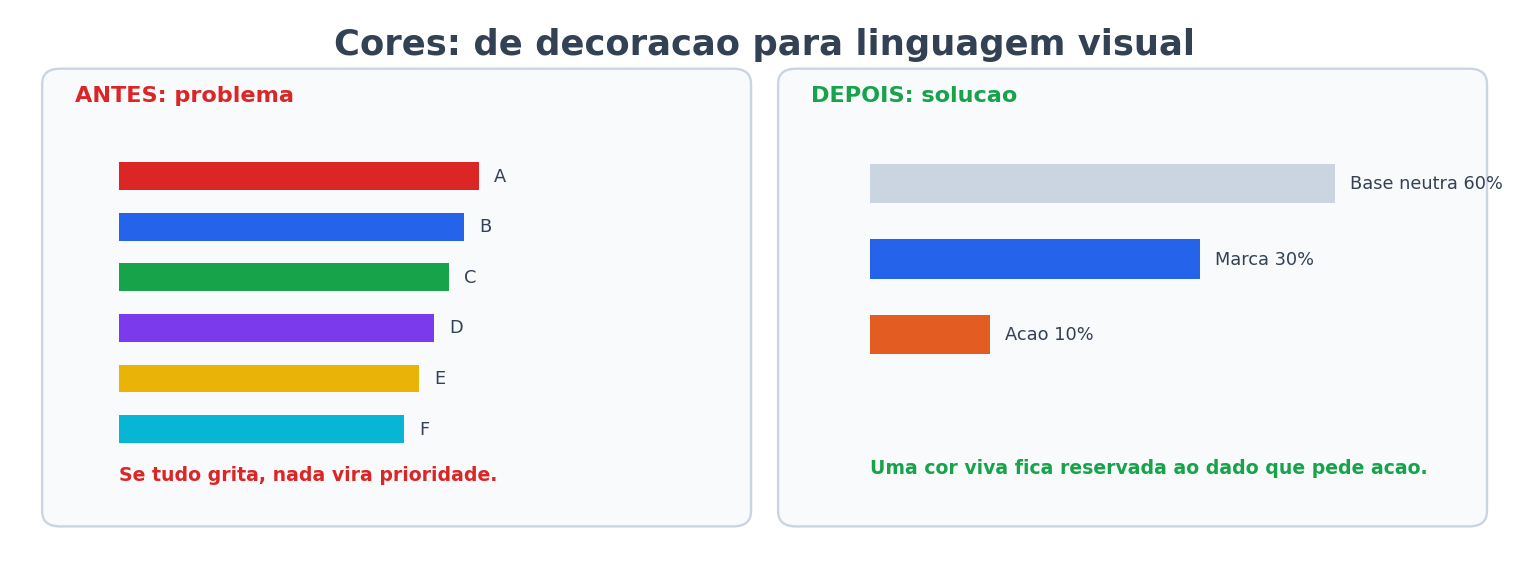
\includegraphics[width=0.58\textwidth]{semana_especial/outputs/cmp_cap1_cores.png}
\caption{Paleta de referência para dashboards. Cada cor tem uma função semântica única. Gráfico gerado pelo script \texttt{auto\_eda\_demo.py}.}
\end{figure}

\begin{BoardBox}[title=Paleta de 8 Funções --- Referência Rápida]
\begin{tabular}{@{}p{0.25cm}lll@{}}
\toprule
& \textbf{Hex} & \textbf{Função} & \textbf{Quando usar} \\
\midrule
\colorbox{colDestaque}{\phantom{M}} & \texttt{\#E35D22} & Destaque / ação urgente & O dado mais importante do dashboard \\
\colorbox{colPrimaria}{\phantom{M}} & \texttt{\#2563EB} & Primária / navegação    & Barras de base, links, filtros \\
\colorbox{colPositivo}{\phantom{M}} & \texttt{\#16A34A} & Positivo / meta atingida & Setas de alta, gaps positivos, badges OK \\
\colorbox{colAlerta}{\phantom{M}}   & \texttt{\#DC2626} & Alerta / falha / risco  & Abaixo da meta, KPI crítico \\
\colorbox{colAtencao}{\phantom{M}}  & \texttt{\#EAB308} & Atenção / monitorar     & Perto do limite, 80--99\% da meta \\
\colorbox{colNeutra}{\phantom{M}}   & \texttt{\#64748B} & Neutra / base           & Eixos, grades, texto secundário \\
\colorbox{colMarca}{\phantom{M}}    & \texttt{\#0B3D2E} & Marca / fundo escuro    & Header, rodapé, modo dark \\
\colorbox{colBgClaro}{\phantom{M}}  & \texttt{\#E2E8F0} & Background / fundo      & Área de trabalho do dashboard \\
\bottomrule
\end{tabular}
\end{BoardBox}

\paragraph{Acessibilidade e daltonismo.}
8\% dos homens e 0,5\% das mulheres têm alguma forma de daltonismo. O tipo mais comum é o deuteranopia (vermelho--verde). Regras práticas: (1) nunca use vermelho e verde como únicos diferenciadores --- adicione ícone de alta/baixa ou rótulo de texto; (2) use ferramentas como \textit{Color Oracle} ou \textit{Coblis} para simular; (3) o par azul--laranja tem alto contraste para daltonismo vermelho--verde e é a combinação padrão de grande parte dos dashboards corporativos.

\paragraph{Cor no Tableau e no QuickSight.}
No Tableau: \texttt{Format} $\to$ \texttt{Color} $\to$ \texttt{Edit Colors} define a paleta da view; use \texttt{Custom Diverging} para heatmaps; use \texttt{Single Color} com opacidade para barras onde o comprimento é o dado. No QuickSight: paletas são definidas no \textit{Theme JSON} e aplicadas globalmente no dataset; campos calculados com `ifelse` podem forçar cor semântica por condição.

% =============================================================
\section{Caminho do Olhar: Analista, Gerente e CEO}
\label{sec:olhar}
% =============================================================

Cada perfil de leitor olha para um dashboard em uma ordem diferente. Ignorar isso é o motivo pelo qual dashboards perfeitamente analíticos falham na sala de board. Entender o caminho do olhar de cada perfil é tão importante quanto escolher o gráfico certo.

\paragraph{O padrão F (analista).}
Pesquisas de eye-tracking de Jakob Nielsen (2006, \textit{Eyetracking Web Usability}) mostram que leitores técnicos percorrem o conteúdo em um padrão em forma de F: (1) leem a linha superior completa; (2) voltam ao início e leem a segunda linha; (3) varrem verticalmente o lado esquerdo em busca de palavras-chave. Implicação para dashboards: \textbf{coloque os dados mais importantes na primeira linha e no canto superior esquerdo}. O analista vai ler tudo, mas a ordem vai moldar o que ele interpreta como importante.

\paragraph{O padrão Z (executivo).}
O executivo com 5 minutos por dia varre o dashboard em Z: canto superior esquerdo $\to$ canto superior direito $\to$ diagonal $\to$ canto inferior esquerdo $\to$ canto inferior direito. Implicação: \textbf{Big Number + título-mensagem no topo esquerdo; Call to Action no rodapé direito; gráfico mais importante na diagonal}.

\begin{BoardBox}[title=Layout em Z para Dashboard Executivo]
\begin{verbatim}
[BIG NUMBER + Big Idea]  ->  [KPI2 | KPI3]
        diagonal
[Grafico diagnostico]    ->  [CALL TO ACTION]
\end{verbatim}
Percurso: (1) KPI principal com delta vs meta; (2) título-mensagem já conta a história;
(3) gráfico de diagnóstico para quem quer o detalhe; (4) CTA com verbo + prazo.
\end{BoardBox}

\begin{figure}[H]
\centering
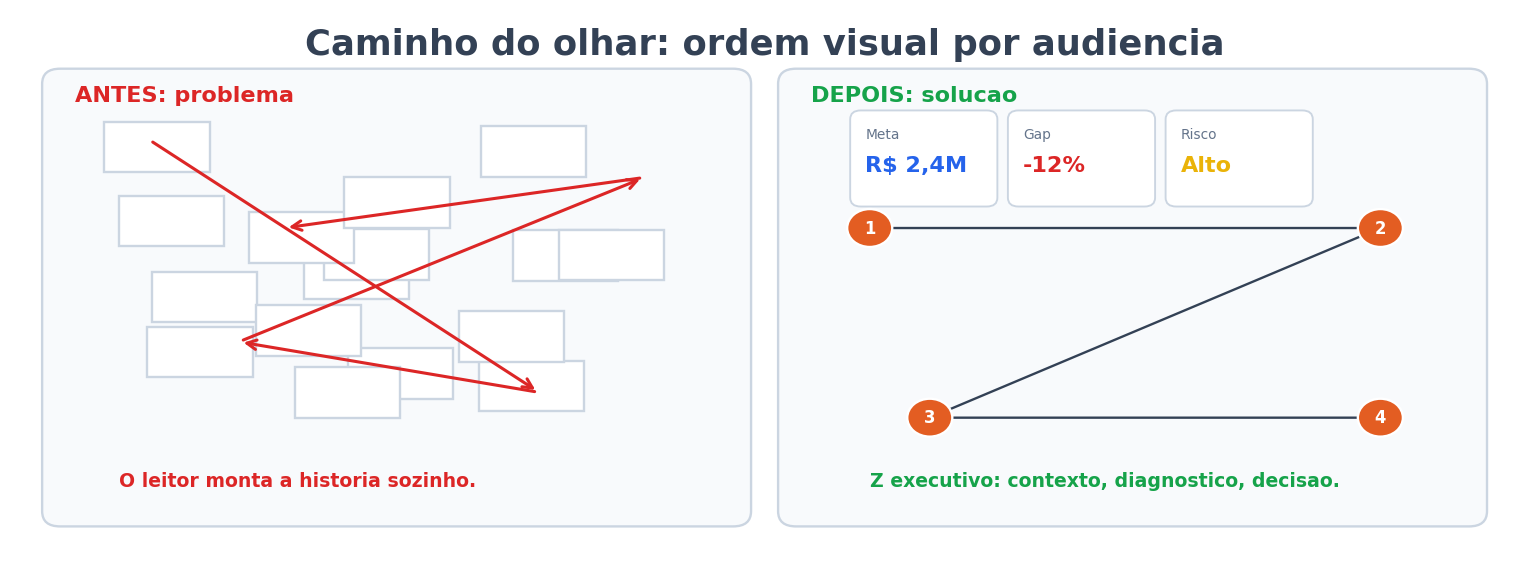
\includegraphics[width=0.58\textwidth]{semana_especial/outputs/cmp_cap1_olhar.png}
\caption{Caminho do olhar por perfil. Use esta figura em aula para mostrar que o mesmo dashboard pode falhar se a ordem visual não combinar com a audiência: o analista lê em F, o executivo varre em Z, e o gerente procura KPI, exceção e tabela de detalhe.}
\end{figure}

\paragraph{Perfil CEO: scanning semântico.}
O CEO não lê gráficos --- ele lê \emph{títulos}. Se os 4 títulos do dashboard entregam as mensagens, o CEO tomou a decisão antes de olhar qualquer eixo. A regra prática: todos os títulos de gráficos em linguagem de manchete de jornal. ``Gráfico de Barras'' $\to$ não. ``Sul lidera com 2,4$\times$ a média'' $\to$ sim.

\paragraph{Perfil gerente/gestor: diagonal + tabela.}
O gerente quer confirmar a hipótese que já tem. Ele vai direto ao gráfico que trata do seu KPI, verifica se o número confirma o que sente, e depois olha a tabela analítica no rodapé para entender as exceções. Implicação: \textbf{ofereça sempre uma tabela de detalhe no rodapé} --- ela não polui o design (ocupa a parte inferior que o executivo ignora) mas salva o gerente de tomar uma decisão com dado incompleto.

\paragraph{Perfil analista: leitura completa em espiral.}
O analista começa no Big Number, vai para o scatter, tenta reproduzir o cálculo, encontra a nota metodológica, cruza com a tabela, e só então forma uma opinião. Para esse perfil, inclua: (1) definição de todas as métricas em tooltip ou nota de rodapé; (2) período de referência explícito; (3) fonte dos dados.

% =============================================================
\section{Carga Cognitiva e Dashboard Cognitivo}
\label{sec:cognitivo}
% =============================================================

A \textbf{teoria da carga cognitiva} (Sweller, 1988) distingue três tipos de carga mental que afetam a absorção de informação. Entender isso explica por que dashboards muito elaborados technicamente falham na comunicação.

\begin{BoardBox}[title=Os 3 Tipos de Carga Cognitiva]
\begin{enumerate}
  \item \textbf{Carga intrínseca:} complexidade inerente ao conteúdo (o dado em si é complicado? a análise exige raciocínio?). Você não pode reduzir isso sem simplificar a análise.
  \item \textbf{Carga extrínseca (extraneous):} esforço causado pelo design ruim. Legenda separada que exige desvio do olhar; cores sem propósito que forçam decodificação; texto e gráfico contradizendo-se. Isso é \textbf{eliminável} com bom design.
  \item \textbf{Carga germane (útil):} esforço que forma aprendizado e schema mental. É o que sobra quando você elimina a carga extrínseca. Você quer maximizar isso.
\end{enumerate}
\smallskip
\textbf{Objetivo do bom design:} eliminar toda a carga extrínseca para liberar capacidade cognitiva para a carga útil.
\end{BoardBox}

\paragraph{Princípios de Gestalt aplicados a dashboards.}
A psicologia da Gestalt descreve como o cérebro organiza elementos visuais em padrões. Cinco princípios diretos:

\begin{BoardBox}[title=Gestalt em Dashboards]
\begin{tabular}{@{}lp{4.2cm}p{5.8cm}@{}}
\toprule
\textbf{Princípio} & \textbf{O que significa} & \textbf{Aplicação prática} \\
\midrule
Proximidade   & Elementos próximos parecem relacionados  & KPIs do mesmo tema agrupados com espaço em branco entre grupos \\
Similaridade  & Elementos parecidos parecem relacionados & Mesma cor = mesma categoria; mesmo formato = mesma hierarquia \\
Fechamento    & O cérebro completa formas incompletas    & Enclosure (caixa) ao redor de KPIs = grupo implícito sem linha pesada \\
Continuidade  & O olho segue linhas e padrões de fluxo  & Gráfico de linhas sugere tendência; use linhas de referência \\
Figura-fundo  & Um elemento se destaca, o resto recua   & 1 cor de destaque em fundo cinza é pura figura-fundo \\
\bottomrule
\end{tabular}
\end{BoardBox}

\paragraph{Dashboard cognitivo: definição.}
Um dashboard cognitivo (termo popularizado por Stephen Few em \textit{Show Me the Numbers}, 2012) é aquele que foi projetado para \emph{minimizar a carga extrínseca e maximizar a carga germane}: título-mensagem que já entrega o insight; cor de destaque que guia o olho; hierarquia visual clara (importante grande, secundário pequeno); remoção de todo chartjunk; e estrutura narrativa que replica o processo de decisão da audiência-alvo.

\begin{figure}[H]
\centering
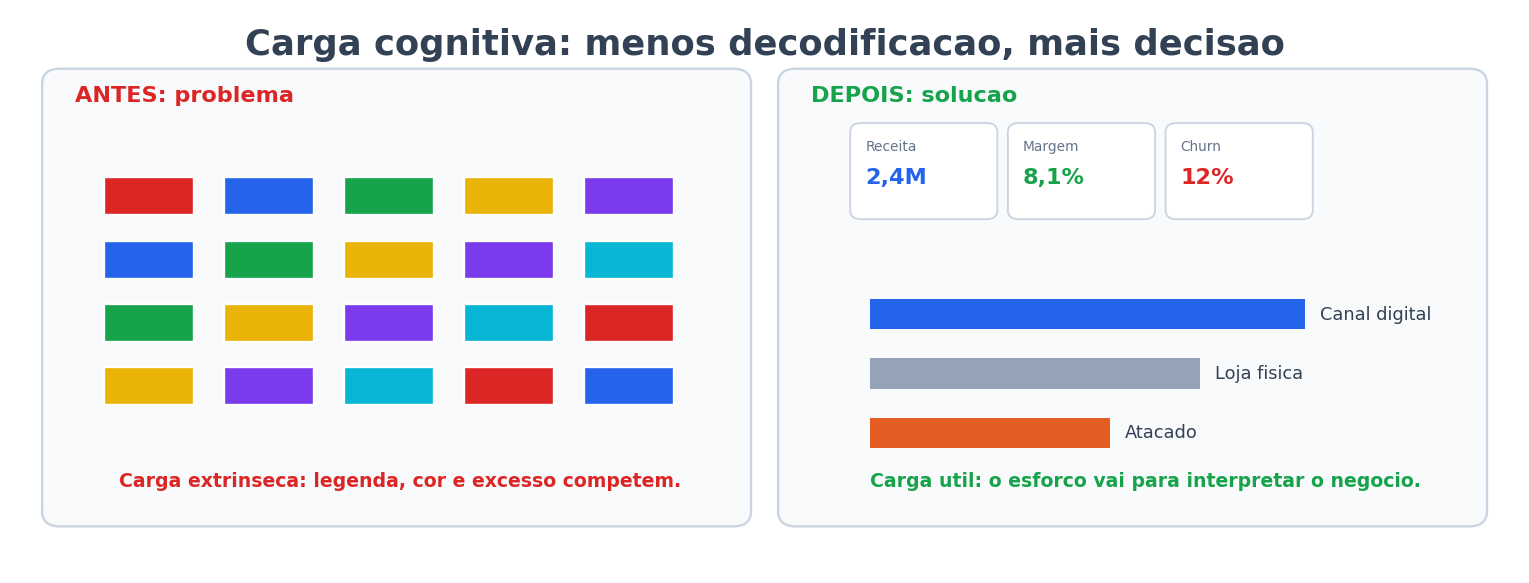
\includegraphics[width=0.58\textwidth]{semana_especial/outputs/cmp_cap1_carga.png}
\caption{Carga cognitiva aplicada a dashboards. À esquerda, o leitor gasta energia decodificando cores, formas e excesso de gráficos; à direita, a energia mental é transferida para entender o problema e decidir.}
\end{figure}

\paragraph{Número mágico 7 ± 2.}
George Miller (1956) demonstrou que a memória de trabalho humana processa 7 (mais ou menos 2) objetos simultâneos. Para dashboards: máximo de 7 KPIs na tela inicial; máximo de 7 categorias por gráfico (agrupe o restante em ``Outros''); máximo de 7 cores distintas numa paleta. Acima desses limites, a interpretação falha mesmo com dados corretos.

% =============================================================
\section{Insights Informativos}
\label{sec:insight_info}
% =============================================================

Um insight informativo é uma observação extraída dos dados que \textbf{aumenta o entendimento} de uma situação mas \emph{não orienta uma ação específica e imediata}. Ele tem valor: reduz incerteza, confirma hipóteses, fornece contexto. O problema começa quando o analista entrega \emph{apenas} insights informativos numa reunião executiva --- porque executivos não precisam de mais informação, precisam de mais clareza sobre o que fazer.

\begin{BoardBox}[title=Características de um Insight Informativo]
\begin{enumerate}
  \item \textbf{Descreve um padrão real:} algo que estava oculto nos dados e que a audiência não sabia.
  \item \textbf{É factual e verificável:} pode ser reproduzido com os mesmos dados.
  \item \textbf{Não tem urgência intrínseca:} ``interessante, mas e daí?'' é a reação esperada.
  \item \textbf{Serve de base para insights acionáveis:} todo bom insight acionável parte de um informativo.
\end{enumerate}
\end{BoardBox}

\textbf{Exemplos de insights informativos:}

\begin{itemize}
  \item ``A distribuição de Exam\_Score é aproximadamente normal (média 67,2; DP 3,9), o que indica que o dataset não tem viés de seleção severo.''
  \item ``Frequência (Attendance) tem a maior correlação com a nota final ($r = 0{,}58$), acima de horas de estudo ($r = 0{,}45$).''
  \item ``Clientes do segmento Premium têm ticket médio 3,2$\times$ maior que o segmento Standard.''
  \item ``O churn em janeiro de 2025 foi 12\% --- o maior dos últimos 24 meses.''
\end{itemize}

Insights informativos são valiosos em relatórios de EDA, em apresentações para times técnicos e em bases de conhecimento internas. O erro é confundi-los com o produto final de uma análise para a diretoria.

\begin{figure}[H]
\centering
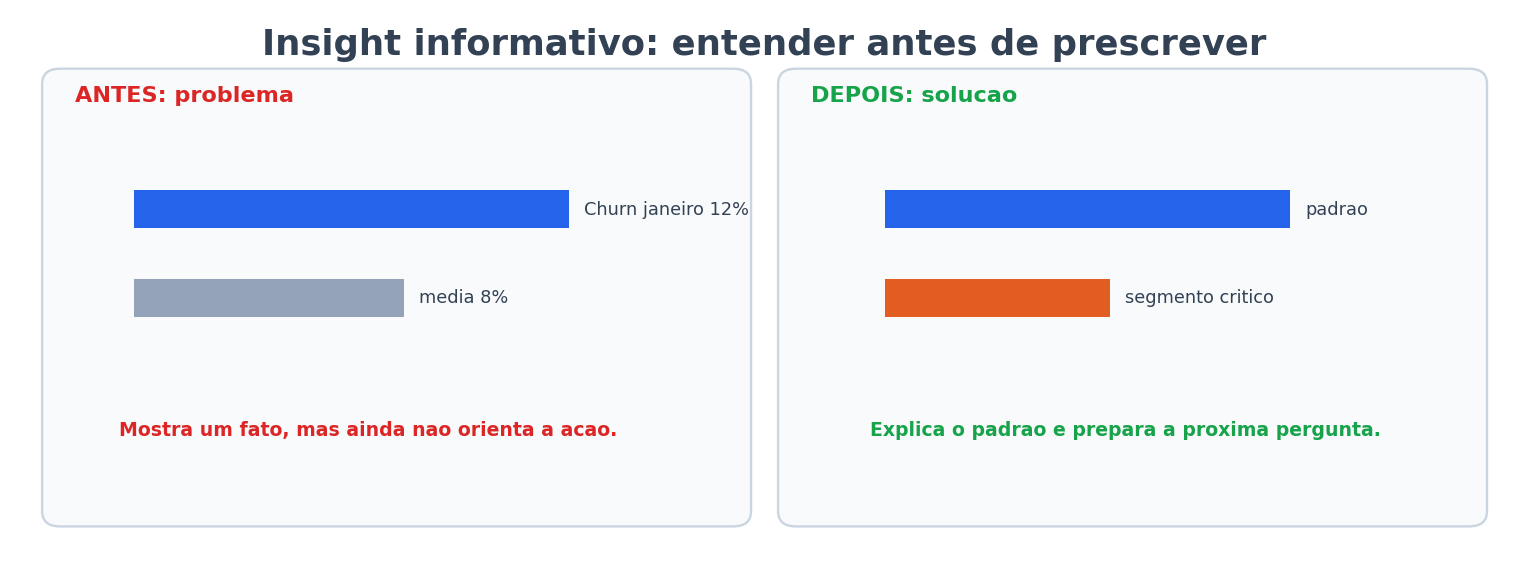
\includegraphics[width=0.58\textwidth]{semana_especial/outputs/cmp_cap1_insight_info.png}
\caption{Insight informativo em dashboard. Ele melhora o entendimento, mas ainda deixa perguntas executivas em aberto: gravidade, responsável, ação e impacto.}
\end{figure}

% =============================================================
\section{Insights Acionáveis: Do Dado à Decisão}
\label{sec:insight_acion}
% =============================================================

Este é o tópico central de qualquer analista que trabalha para a tomada de decisão. Um insight acionável \textbf{prescreve uma ação específica, direcionada a um responsável, com estimativa de impacto e prazo}. Ele não descreve o passado --- ele orienta o futuro. A diferença entre analistas júnior e sênior, na prática bancária e em qualquer grande corporação, é exatamente a capacidade de transformar observações numéricas em recomendações que mudam o comportamento de alguém.

\begin{BoardBox}[title=Fórmula do Insight Acionável --- 5 Componentes]
\begin{enumerate}
  \item \textbf{Observação:} padrão não-óbvio extraído dos dados.
  \item \textbf{Evidência:} o dado que sustenta a observação (com magnitude e significância).
  \item \textbf{Causa raiz (quando possível):} por que isso está acontecendo?
  \item \textbf{Ação prescrita:} verbo + objeto + quantidade + canal.
  \item \textbf{Impacto estimado:} resultado esperado em métrica de negócio + prazo.
\end{enumerate}
\smallskip
\textbf{Template:} ``[Observação] porque [evidência]. Se [ação prescrita] então [impacto estimado] em [prazo], responsável: [stakeholder].''
\end{BoardBox}

\paragraph{Por que a maioria dos analistas não consegue fazer isso.}
O bloqueio é conceitual: o analista foi treinado para \emph{descrever} dados, não para \emph{prescrever} ações. Descrever é seguro --- ninguém erra ao reportar que ``as vendas caíram 8\%''. Prescrever exige entender o negócio, assumir uma hipótese causal e aceitar que pode estar errado. O sênior aceita esse risco porque o valor gerado pela ação certa supera muito o custo de estar errado em uma recomendação específica.

\paragraph{Exemplos completos --- 8 domínios.}

Os exemplos a seguir seguem a estrutura de 5 componentes. Leia devagar: a diferença entre o insight informativo (coluna ``sem ação'') e o acionável (coluna ``com ação'') é a diferença de impacto na carreira de um analista.

\medskip
\textbf{Exemplo 1 --- Banco: análise de churn de cartão de crédito}

\textit{Informativo:} ``Clientes com menos de 20 transações por ano têm taxa de churn de 38\%, vs 6\% para clientes com mais de 50 transações.''

\textit{Acionável:} ``Clientes com frequência de uso $<$ 20 trans/ano e saldo médio $<$ R\$2k têm 38\% de probabilidade de cancelamento --- 3,4 pp acima da base. Acionar campanha de reengajamento personalizado via app (cashback + limite temporário) para os 8.200 clientes nesse perfil pode reverter 30\% do churn projetado, preservando R\$1,4M em receita de juros e anuidade nos próximos 12 meses. Responsável: Gerência de CRM. Prazo de implementação: 3 semanas.''

\medskip
\textbf{Exemplo 2 --- Varejo: pricing de produto}

\textit{Informativo:} ``Produtos com desconto $>$ 20\% têm margem média de $-4\%$.''

\textit{Acionável:} ``Descontos acima de 20\% em Linha Branca na Região Sul destroem R\$120k de margem por trimestre sem aumentar o volume de unidades (elasticidade próxima de zero na análise de regressão). Capear o desconto máximo em 12\% mantém a competitividade de preço percebida e projeta recuperação de R\$85k de margem trimestral. Responsável: Gerência Comercial Sul. Prazo: implementar na campanha de inverno (início de julho).''

\medskip
\textbf{Exemplo 3 --- RH: turnover de TI}

\textit{Informativo:} ``O departamento de TI tem turnover de 28\%, acima da média corporativa de 12\%.''

\textit{Acionável:} ``Engenheiros de TI com menos de 2 anos de empresa e sem promoção nos últimos 36 meses têm 3$\times$ mais probabilidade de saída que a média (28\% vs 9\%). Esse perfil representa 41 funcionários. Implantar programa de mentoria acelerada + revisão de faixa salarial para esse grupo específico pode reduzir o turnover de 28\% para 15\%, economizando R\$270k/ano em custo de reposição (R\$18k/funcionário $\times$ 15 saídas evitadas). Responsável: HRBP de TI + Diretor de Engenharia. Prazo: começar em 30 dias para impactar a janela de avaliação semestral.''

\medskip
\textbf{Exemplo 4 --- Saúde: readmissão hospitalar}

\textit{Informativo:} ``Pacientes com diabetes + hipertensão têm taxa de readmissão em 30 dias de 34\%.''

\textit{Acionável:} ``Pacientes diabéticos com HbA1c $>$ 9 e diagnóstico de HAS que receberam alta sem consulta de retorno agendada têm 34\% de readmissão em 30 dias vs 8\% quando o retorno está agendado. Implementar protocolo de agendamento obrigatório na alta para os 1.200 pacientes nesse perfil anual pode evitar 312 readmissões, economizando R\$3,7M (R\$12k/internação), além de melhorar o indicador de qualidade AHRQ-PSI. Responsável: Gerência de Assistência. Prazo: protocolo ativo no próximo semestre.''

\medskip
\textbf{Exemplo 5 --- E-commerce: logística}

\textit{Informativo:} ``O estado do Amazonas tem atraso médio de 4,7 dias acima da estimativa.''

\textit{Acionável:} ``Pedidos de Eletrônicos em AM com prazo estimado $<$ 7 dias chegam em média 4,7 dias atrasados, gerando review médio de 2,8 estrelas e taxa de devolução 18\% acima da média. Substituir a transportadora atual por operador regional com SLA de 5 dias para essa rota reduz o atraso estimado em 70\%, projeta melhora do review para 4,1 estrelas e reduz devoluções em R\$95k/semestre. Responsável: Gerência de Logística. Prazo: RFP para transportadora em 45 dias.''

\medskip
\textbf{Exemplo 6 --- Fintech: crédito}

\textit{Informativo:} ``A inadimplência de empréstimo pessoal cresceu 3 pp em Q1/2026.''

\textit{Acionável:} ``Clientes de empréstimo pessoal com renda variável (profissional autônomo) que acessaram o produto em fevereiro/março têm inadimplência de 19\%, contra 7\% para clientes com renda fixa. O crescimento de 3 pp na inadimplência total é explicado em 78\% por esse segmento (análise de decomposição). Ajustar a política de crédito para limitar o LTV de empréstimo pessoal a 60\% da renda variável comprovada pode reduzir a inadimplência desse perfil de 19\% para 10\%, preservando R\$4,2M em provisão de crédito no próximo trimestre. Responsável: Gerência de Risco de Crédito. Prazo: vigência imediata para novas contratações.''

\medskip
\textbf{Exemplo 7 --- Educação (dataset StudentPerformance)}

\textit{Informativo:} ``Frequência (Attendance) tem correlação de 0,58 com Exam\_Score, sendo o preditor mais forte entre as variáveis numéricas.''

\textit{Acionável:} ``Alunos com frequência $<$ 75\% nos meses de março--abril têm nota final média 9,3 pts abaixo da média geral (67,2), e 34\% deles reprovam. Implementar sistema de alerta automático por WhatsApp para responsáveis quando o aluno atingir 3 faltas consecutivas pode recuperar 40\% desses alunos (baseado em piloto de 2024), reduzindo a taxa de reprovação de 8\% para 4,8\%, equivalendo a 216 alunos aprovados adicionais por semestre. Responsável: Coordenação Pedagógica + TI. Prazo: sistema ativo no início do semestre seguinte.''

\medskip
\textbf{Exemplo 8 --- Marketing digital: aquisição}

\textit{Informativo:} ``O CAC médio pelo canal Google Ads é R\$48, contra R\$31 pelo canal Organic.''

\textit{Acionável:} ``O canal Google Ads tem CAC 55\% maior que o orgânico, mas o LTV dos clientes adquiridos por Google Ads é apenas 8\% maior (R\$320 vs R\$296). O ROI ajustado ao LTV do canal pago é negativo ($-$4\%) no primeiro ano. Redirecionar 40\% do orçamento de Google Ads para SEO/Content durante 6 meses projeta redução do CAC médio de R\$48 para R\$35, com impacto de $-$12\% no volume de aquisição no curto prazo mas retorno positivo a partir do mês 8. Responsável: Gerência de Marketing. Prazo: próximo ciclo de orçamento (Q3 2026).''

\paragraph{Como treinar a habilidade de gerar insights acionáveis.}
O caminho mais rápido é forçar a pergunta ``\emph{e daí?}'' sobre cada dado encontrado. Toda vez que você escrever uma observação, pergunte: ``E daí?'' até chegar num verbo de ação ligado a um responsável. Veja a cadeia:

\begin{BoardBox}[title=A Cadeia ``E Daí?'' --- Exercício Prático]
\textbf{Observação inicial:} ``O churn subiu 3\%.'' \quad \textbf{E daí?}\\
\textbf{Nível 2:} ``Clientes do segmento X estão cancelando mais.'' \quad \textbf{E daí?}\\
\textbf{Nível 3:} ``Clientes do segmento X com produto Y cancelam 4$\times$ mais no 3$^\circ$ mês.'' \quad \textbf{E daí?}\\
\textbf{Nível 4:} ``O problema é que o onboarding do produto Y não é completado por 60\% dos clientes.'' \quad \textbf{E daí?}\\
\textbf{Insight acionável:} ``Criar fluxo de onboarding guiado no app para produto Y, com nudge no dia 15, pode reduzir o churn do segmento X de 18\% para 8\%, preservando R\$XX em ARR. Responsável: PM + CRM. Prazo: 4 semanas.''
\end{BoardBox}

\begin{figure}[H]
\centering
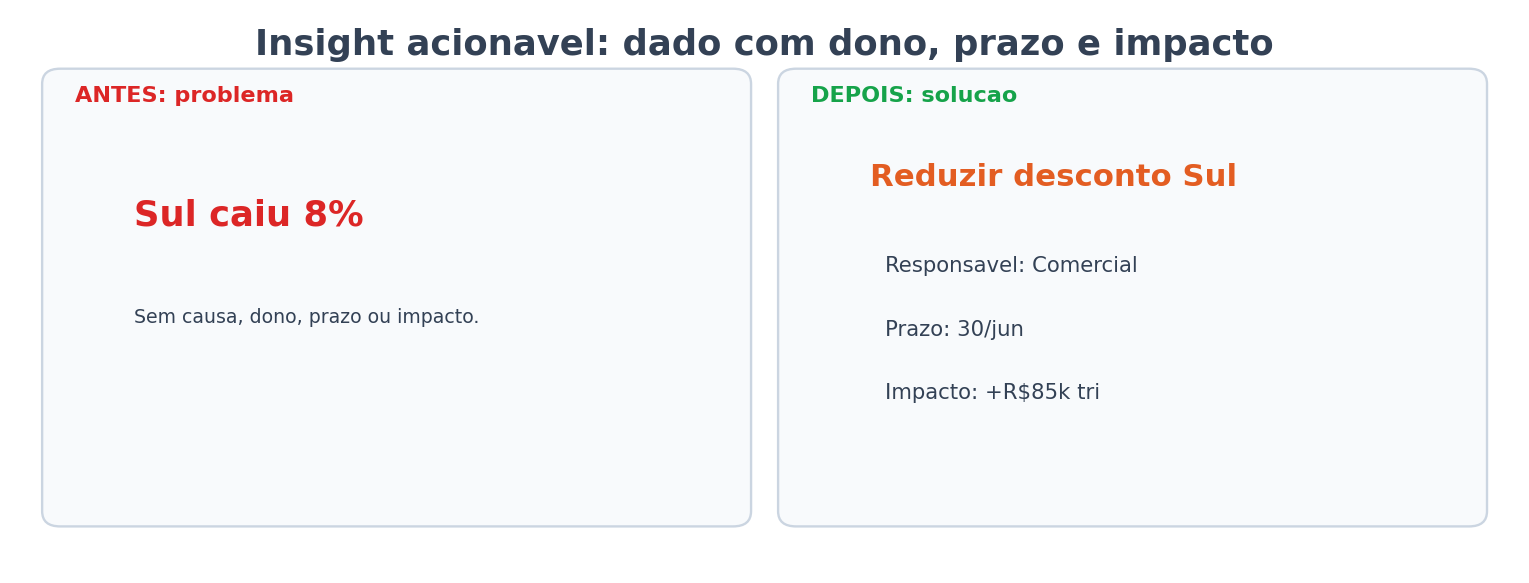
\includegraphics[width=0.58\textwidth]{semana_especial/outputs/cmp_cap1_insight_acionavel.png}
\caption{Dashboard sem ação versus dashboard com insight acionável. O segundo não apenas descreve o problema: ele explicita o que fazer, quem deve fazer, até quando e qual impacto esperado.}
\end{figure}

% =============================================================
\section{Dashboard as Code: AWS e QuickSight}
\label{sec:daac}
% =============================================================

\textbf{Dashboard as Code (DaC)} é a prática de definir, versionar e publicar dashboards inteiramente via código e infraestrutura como código (IaC), eliminando configuração manual via interface gráfica. Os benefícios diretos para um time de analytics bancário são: rastreabilidade via Git, reprodutibilidade entre ambientes (dev/homol/prod), revisão de mudanças por Pull Request, e orquestração programática de dezenas de dashboards.

\paragraph{AWS QuickSight e as APIs de criação.}
O QuickSight expõe uma API REST completa (\textit{aws quicksight} via Boto3 ou CLI) que permite criar e atualizar todos os recursos: datasets, análises, dashboards e permissões. Os objetos principais na hierarquia são:

\begin{BoardBox}[title=Hierarquia de Objetos no QuickSight]
\begin{tabular}{@{}llp{6.5cm}@{}}
\toprule
\textbf{Objeto} & \textbf{API} & \textbf{Descrição} \\
\midrule
DataSource    & \texttt{create-data-source}    & Conexão ao S3/Redshift/Athena/RDS \\
DataSet       & \texttt{create-data-set}       & Schema, joins, campos calculados, filtros de linha \\
Analysis      & \texttt{create-analysis}       & Canvas de edição (não publicado) \\
Dashboard     & \texttt{create-dashboard}      & Versão publicada de uma Analysis \\
Template      & \texttt{create-template}       & Snapshot de uma Analysis reutilizável cross-account \\
Theme         & \texttt{create-theme}          & Paleta de cores, fontes e layout globais \\
\bottomrule
\end{tabular}
\end{BoardBox}

\paragraph{Fluxo conceitual do Dashboard as Code.}
Para esta aula, o importante não é decorar código de Boto3 ou CDK. O ponto central é entender que o dashboard deixa de ser uma peça manual feita no clique e passa a ser um artefato governado: nasce de uma regra de negócio, é versionado, revisado, homologado e publicado com rastreabilidade.

\begin{figure}[H]
\centering
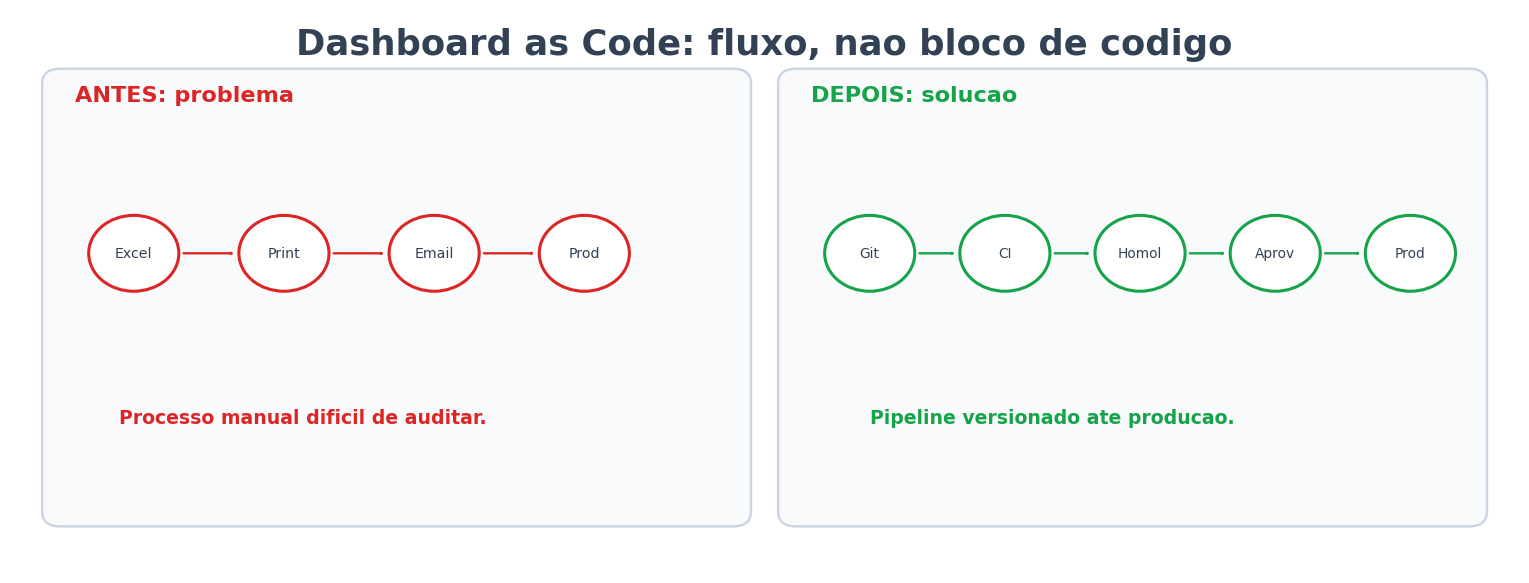
\includegraphics[width=0.58\textwidth]{semana_especial/outputs/cmp_cap1_dac.png}
\caption{Fluxo conceitual de Dashboard as Code. A criação programática só faz sentido quando protege governança: regra de negócio clara, definição versionada, revisão por pares, homologação e publicação controlada.}
\end{figure}

\paragraph{Fluxo de trabalho DaC com Git.}
O padrão recomendado para times de analytics em bancos: (1) \texttt{feature/dashboard-churn} branch; (2) código Python com definição de datasets + análise em JSON (exportado via \texttt{describe-analysis-definition}); (3) PR com revisão de outro analista; (4) merge em \texttt{main} dispara GitHub Actions que chama \texttt{boto3.update\_dashboard}; (5) tags de versão correspondem a versões do QuickSight.

\paragraph{Asset Bundle Export/Import.}
Para migração entre contas (dev $\to$ prod) sem recriar tudo manualmente, o QuickSight oferece desde 2023 o \textbf{Asset Bundle} API: exporta análises, dashboards, datasets e temas em JSON e importa em outra conta com substituição de ARNs. Isso é o equivalente ao \texttt{terraform plan/apply} para dashboards.

% =============================================================
\section{AED Automática: Bibliotecas, Relatórios e Interpretação}
\label{sec:autoeda}
% =============================================================

As bibliotecas de AED automática (profiling) fazem em uma linha o que levaria horas de código manual: calculam estatísticas descritivas, detectam outliers, mapeiam correlações, identificam dados ausentes, avaliam distribuições e geram relatório HTML completo. Elas não substituem a análise --- substituem a parte mecânica para que o analista foque na interpretação.

\begin{BoardBox}[title=Principais Bibliotecas de AED Automática (Python)]
\begin{tabular}{@{}lp{3.5cm}p{5.8cm}@{}}
\toprule
\textbf{Biblioteca} & \textbf{Melhor para} & \textbf{Diferencial} \\
\midrule
\texttt{ydata-profiling} & Relatório completo solo & 1 linha; HTML interativo; detecta correlações, outliers, duplicatas, alertas de qualidade \\
\texttt{sweetviz}        & Comparação de grupos    & Visualiza diferenças entre treino/teste ou segmentos lado a lado; target analysis \\
\texttt{autoviz}         & Visualizações rápidas   & Gera gráficos automaticamente sem HTML; bom para exploração rápida \\
\texttt{D-Tale}          & Exploração interativa   & Interface web local tipo Excel interativo; edição de dados em tempo real \\
\texttt{lux}             & Recomendação automática & Sugere visuais relevantes contextualizados ao DataFrame; integra Jupyter \\
\bottomrule
\end{tabular}
\end{BoardBox}

\paragraph{Como ler um relatório automático.}
Nesta aula, não precisamos decorar comandos. O que importa é saber interpretar o HTML produzido por essas ferramentas. Primeiro olhe os \textbf{alertas de qualidade}: dados ausentes, duplicatas, cardinalidade alta e colunas constantes. Depois leia as \textbf{distribuições}: assimetria, outliers e concentração. Em seguida, veja \textbf{correlações e associações}: elas sugerem hipóteses, mas não provam causalidade. Por fim, transforme o relatório em perguntas de negócio: ``qual variável explica o resultado?'', ``qual grupo merece intervenção?'', ``que dado precisa ser validado antes da decisão?''.

\begin{figure}[H]
\centering
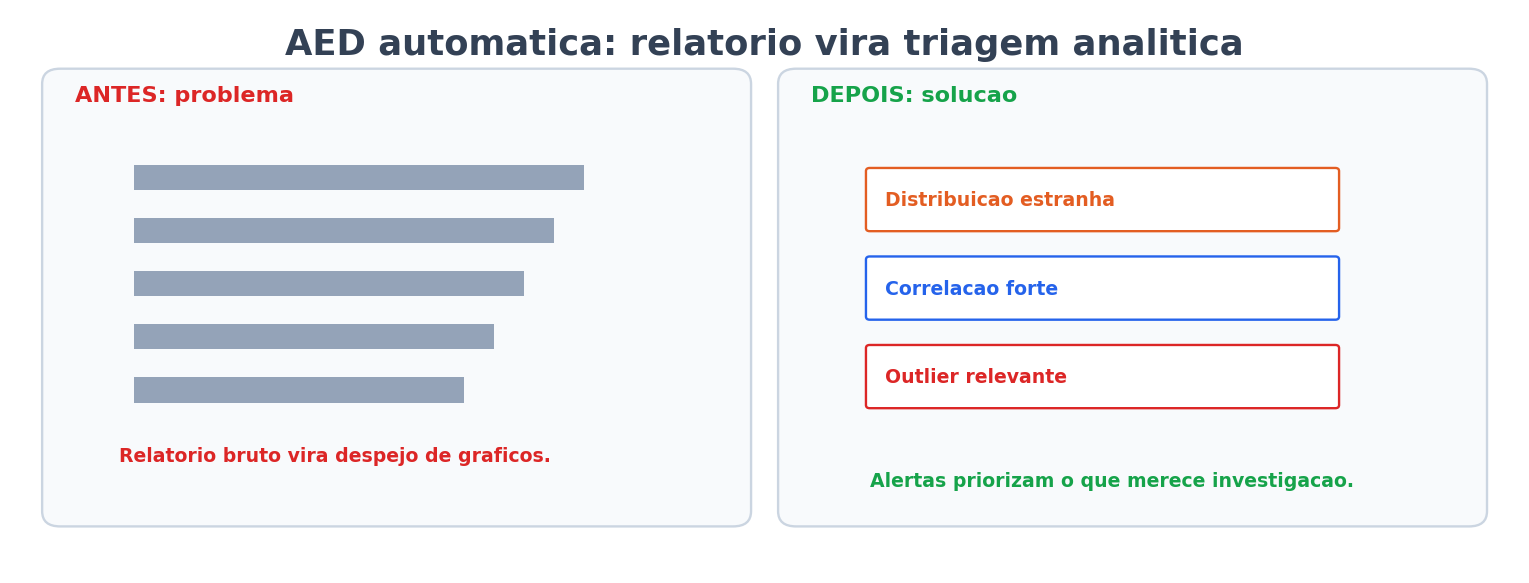
\includegraphics[width=0.58\textwidth]{semana_especial/outputs/cmp_cap1_autoeda.png}
\caption{Fluxo de leitura da AED automática. O HTML é um ponto de partida: ele encontra sinais, mas o analista precisa explicar o significado e formular a próxima pergunta.}
\end{figure}

\paragraph{Exemplo real: StudentPerformanceFactors.csv.}

Rodamos \texttt{ydata-profiling} (modo minimal, 6607 registros, 20 variáveis) e \texttt{sweetviz} no dataset deste curso. Os relatórios HTML estão em \texttt{semana\_especial/outputs/}:
\begin{itemize}
  \item \texttt{ydata\_profiling\_report.html} --- perfil completo com alertas de qualidade, correlações, distribuições
  \item \texttt{sweetviz\_report.html} --- target analysis com Exam\_Score como variável alvo
\end{itemize}

Em aula, use esses relatórios como material de inspeção: eles mostram distribuições, correlações, scatterplots e variáveis categóricas. O PDF mantém apenas o comparativo acima para não repetir quatro figuras exploratórias onde uma síntese visual resolve melhor.

\paragraph{Alertas automáticos que o ydata-profiling detecta.}
O relatório HTML sinaliza automaticamente: variáveis com $>$ 5\% de dados ausentes; colunas com alta correlação ($>$ 0,9) que indicam redundância; variáveis com cardinalidade muito alta (suspeita de ID); distribuições muito assimétricas (candidatas a transformação log); valores constantes ou quase-constantes.

\paragraph{Quando NÃO usar AED automática.}
Quando o dataset tem $>$ 10M de linhas (o relatório trava ou demora demais --- use uma amostra estratificada de 50k--100k linhas); quando as variáveis têm semântica muito específica do negócio que a biblioteca não conhece (ex.: códigos de agência bancária precisam de dicionário manual); quando o objetivo já é confirmatory (você já sabe o que procura --- vá direto).

% =============================================================
\section{Arquitetura de Agentes para AED e Dashboards}
\label{sec:agentes}
% =============================================================

A abordagem de agentes para análise de dados está passando de experimento acadêmico para realidade em grandes bancos e fintechs em 2025--2026. A ideia central é substituir o fluxo manual linear (analista faz EDA $\to$ analista faz perguntas $\to$ analista constrói dashboard) por um \textbf{pipeline orquestrado de agentes especializados}, cada um responsável por uma etapa e passando seu output como contexto estruturado para o próximo.

\paragraph{A arquitetura descrita.}
O pipeline que estamos construindo no banco tem a seguinte cadeia:

\begin{BoardBox}[title=Pipeline Multi-Agente --- Etapas]
\begin{enumerate}
  \item \textbf{Agente Discovery:} lê o contrato de negócio (dores, KPIs, audiência), carrega o dataset, calcula estatísticas descritivas, mapeia correlações, detecta outliers. Output: JSON com contexto estruturado.
  \item \textbf{Agente de Insights:} recebe o JSON do Agente 1, consulta a base especializada de insights (seção 9), e gera insights acionáveis candidatos com score de relevância.
  \item \textbf{Agente de Storyboard:} define Big Idea, estrutura 3 zonas (Contexto/Diagnóstico/Recomendação), monta a sequência de gráficos e os títulos-mensagem.
  \item \textbf{Agente Protótipo:} gera HTML completo do dashboard com Chart.js, auto-contido, com dados reais do dataset. Output: \texttt{prototipo.html}.
  \item \textbf{Agente de Infraestrutura (AWS):} recebe o protótipo aprovado, converte para definição QuickSight (JSON/API), cria DataSet + Analysis + Dashboard via Boto3.
  \item \textbf{Agente de Documentação:} gera changelog, dicionário de métricas e runbook automaticamente a partir dos metadados dos agentes anteriores.
\end{enumerate}
\smallskip
\textbf{Orquestrador:} LangChain / LangGraph / AWS Step Functions (para pipelines produtivos em nuvem).
\end{BoardBox}

\begin{figure}[H]
\centering
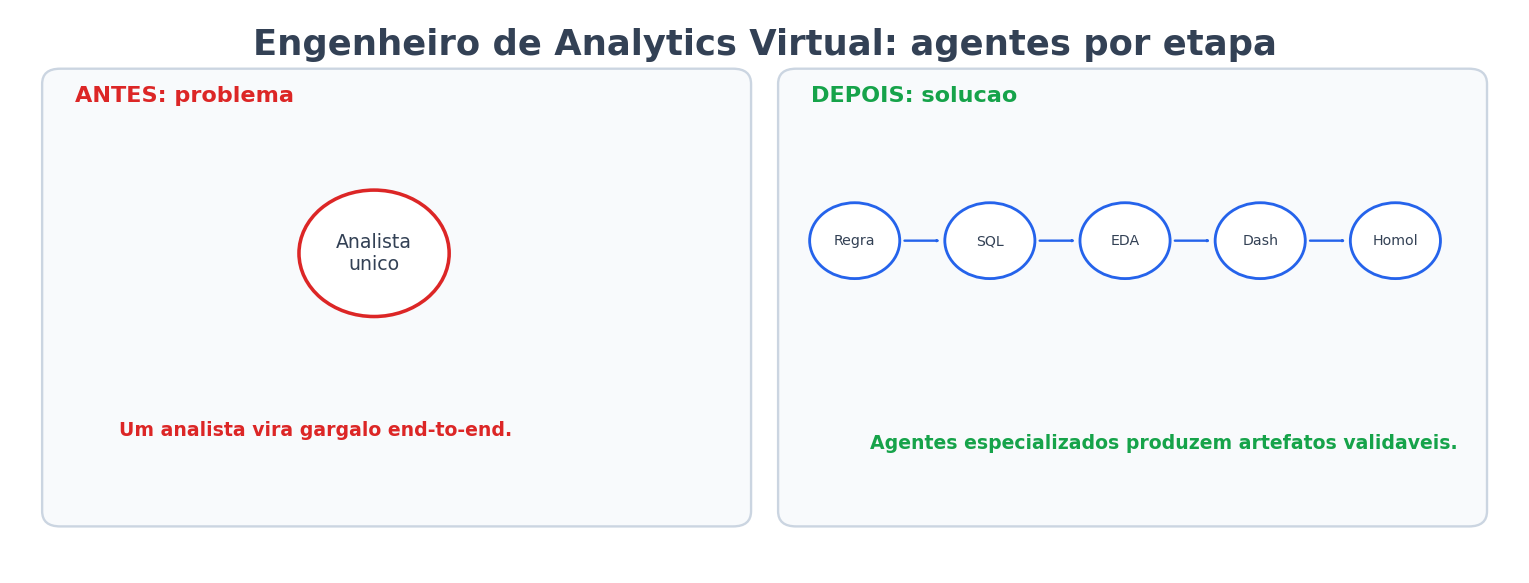
\includegraphics[width=0.58\textwidth]{semana_especial/outputs/cmp_cap1_agentes.png}
\caption{Arquitetura lúdica do Engenheiro de Analytics Virtual. A ideia prática é end-to-end: da regra de negócio até a publicação do dashboard, cada agente produz um artefato que pode ser revisado e homologado.}
\end{figure}

\paragraph{Protótipo gerado pelo pipeline.}

O script \texttt{agente\_prototipo\_html.py} executa os Agentes 1--4 localmente, sem LLM externo, usando apenas pandas e Chart.js. O arquivo \texttt{prototipo\_dashboard\_agente.html} está em \texttt{semana\_especial/outputs/}. Ele demonstra a estrutura que o pipeline mais completo (com LLM) produziria.

\paragraph{Como funcionaria na prática.}
Imagine que a área de negócio pede: ``o churn do cartão Premium subiu e precisamos decidir uma campanha''. O Agente de Negócio transforma isso em contrato: audiência, dor, métrica-alvo, restrições e prazo. O Agente de Dados valida tabelas, chaves, granularidade e qualidade. O Agente SQL cria ou sugere views analíticas. O Agente EDA procura padrões. O Agente de Insights transforma padrões em recomendações. O Agente Storyboard escolhe a sequência narrativa. O Agente Protótipo gera um HTML para homologação rápida. Só depois de aprovado entram os agentes de produção: criação de dataset, dashboard no BI, permissões, documentação e changelog.

\begin{BoardBox}[title=Artefatos por Agente]
\begin{tabular}{@{}lp{8.7cm}@{}}
\toprule
\textbf{Agente} & \textbf{Artefato entregue} \\
\midrule
Negócio & contrato de análise: dor, KPI, audiência, decisão esperada \\
Dados/SQL & tabela, view ou consulta validada com dicionário de métricas \\
EDA & resumo visual de padrões, outliers, correlações e alertas \\
Insights & 2--3 recomendações acionáveis com impacto e responsável \\
Storyboard & Big Idea, zonas do dashboard e títulos-mensagem \\
Protótipo & HTML navegável para homologação com usuário \\
Produção & dashboard publicado, permissões, documentação e versão \\
\bottomrule
\end{tabular}
\end{BoardBox}

\paragraph{Padrões de multi-agente: ReAct, Chain-of-Thought e Tool-Use.}
Três padrões são relevantes para o pipeline de analytics: (1) \textbf{ReAct} (Yao et al., 2022) --- o agente raciocina (\textit{Thought}) e então age (\textit{Action}), iterando até atingir o objetivo; ideal para o Agente de Insights que precisa testar hipóteses. (2) \textbf{Chain-of-Thought} (Wei et al., 2022) --- o agente externaliza o raciocínio passo a passo antes de entregar o output; útil no Agente de Storyboard para justificar cada decisão de layout. (3) \textbf{Tool-Use / Function-Calling} (OpenAI, 2023) --- o agente chama funções externas (Boto3, Tableau API, base de dados) de forma estruturada; é o que habilita o Agente de Infraestrutura a criar dashboards reais no QuickSight.

% =============================================================
\section{Como Criar Insights Acionáveis: Base Especializada}
\label{sec:insight_base}
% =============================================================

O maior gargalo para gerar insights acionáveis em escala (em um time de 20 analistas, para dezenas de produtos) é a \textbf{inconsistência de qualidade}. Cada analista usa sua própria definição do que é um insight, seu próprio template, sua própria escala de urgência. O resultado: 80\% dos ``insights'' entregues são observações descritivas, e os executivos param de ler relatórios de dados.

A solução é criar uma \textbf{base especializada em insights}: um repositório estruturado (tabela, vector store ou knowledge base) que contém exemplos de alta qualidade validados pelo negócio, que serve de referência para analistas humanos e de few-shot context para agentes de IA.

\begin{figure}[H]
\centering
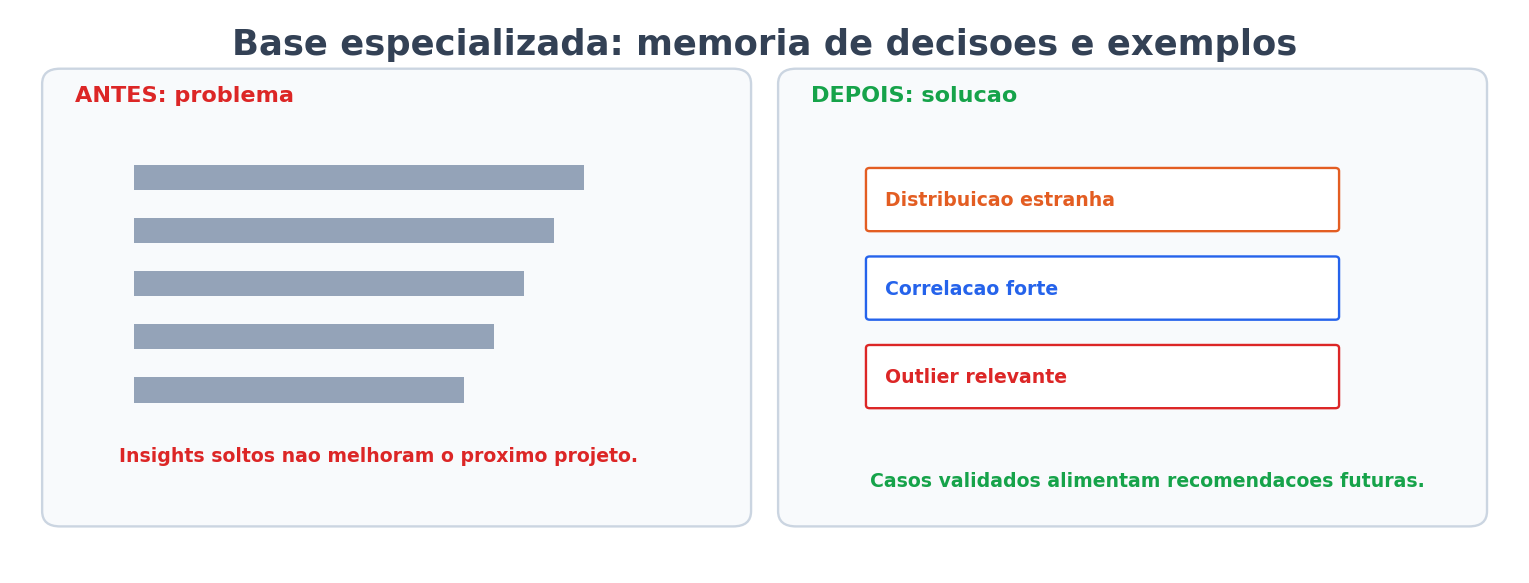
\includegraphics[width=0.58\textwidth]{semana_especial/outputs/cmp_cap1_base_insights.png}
\caption{Base especializada de insights. Ela funciona como memória de qualidade: exemplos validados alimentam novos agentes e padronizam o que a turma deve chamar de insight acionável.}
\end{figure}

\begin{BoardBox}[title=Tabela \texttt{insight\_base}]
\small
\begin{tabular}{@{}p{3.2cm}p{2.2cm}p{5.6cm}@{}}
\toprule
\textbf{Campo} & \textbf{Tipo} & \textbf{Descrição} \\
\midrule
\texttt{insight\_id}    & VARCHAR(20)  & Identificador único (ex.: INS-001) \\
\texttt{dominio}        & VARCHAR(50)  & Área do negócio (Crédito, Varejo, RH\ldots) \\
\texttt{tipo}           & ENUM         & \texttt{acionavel} | \texttt{informativo} \\
\texttt{titulo}         & VARCHAR(200) & Frase-resumo do insight (padrão + ação) \\
\texttt{observacao}     & TEXT         & Padrão detectado com dado concreto \\
\texttt{evidencia}      & TEXT         & Estatística que sustenta (n, correlação, delta) \\
\texttt{causa\_raiz}    & TEXT         & Hipótese causal (quando disponível) \\
\texttt{acao}           & TEXT         & Verbo + objeto + canal + quantidade \\
\texttt{impacto}        & TEXT         & Resultado esperado em métrica de negócio \\
\texttt{stakeholder}    & VARCHAR(100) & Responsável pela ação \\
\texttt{urgencia}       & ENUM         & \texttt{Alta} | \texttt{Media} | \texttt{Baixa} \\
\texttt{prazo\_sugerido}& VARCHAR(50)  & Ex.: ``Q3 2026'', ``próximo semestre'' \\
\texttt{fonte}          & VARCHAR(200) & Dataset / tabela de origem \\
\texttt{validado\_por}  & VARCHAR(100) & Analista ou gestor que validou o insight \\
\texttt{data\_criacao}  & DATE         & Data de geração \\
\texttt{embedding}      & VECTOR(1536) & Embedding semântico para busca por similaridade \\
\bottomrule
\end{tabular}
\end{BoardBox}

\paragraph{Exemplo real gerado pelo pipeline.}

O arquivo \texttt{insight\_base\_exemplo.csv} em \texttt{semana\_especial/outputs/} contém 3 registros gerados automaticamente pelo Agente de Insights sobre o dataset StudentPerformance. A estrutura é a mesma para qualquer domínio.

\paragraph{Como o agente usa a base para gerar novos insights.}
O Agente de Insights (seção anterior) faz o seguinte: (1) calcula as estatísticas do dataset atual (Agente 1); (2) busca na base especializada os 3--5 insights mais similares por domínio + tipo de padrão (busca vetorial por embedding semântico); (3) usa esses exemplos como \textit{few-shot context} no prompt do LLM; (4) o LLM gera um insight acionável seguindo exatamente o schema. A qualidade dos exemplos na base determina diretamente a qualidade dos insights gerados.

\begin{BoardBox}[title=Uso da Base pelo Agente]
Na prática, o agente não ``inventa'' do zero. Ele recebe o contexto do dataset, busca exemplos parecidos na base, compara o padrão atual com casos já validados, e então gera uma recomendação no mesmo formato: observação, evidência, ação, impacto, responsável e prazo. Isso reduz variação de qualidade entre analistas e evita que uma observação descritiva seja vendida como insight.
\end{BoardBox}

\paragraph{Construir a base de forma contínua.}
A base deve crescer com cada projeto: (1) analista gera insights; (2) gestor valida e adiciona o campo \texttt{validado\_por}; (3) após 6 meses, mede-se a taxa de adoção das ações recomendadas e o impacto realizado vs estimado --- isso cria um loop de melhoria contínua na qualidade dos insights gerados.

Em produção na AWS, a base pode ser: uma tabela no DynamoDB (para escrita/leitura rápida por analistas) + uma coleção no Amazon Bedrock Knowledge Base (para busca semântica pelo agente) + um bucket S3 como backup e auditoria.

% =============================================================
\section*{Referências: Cognição, Insights e Automação}
% =============================================================

As referências abaixo estão disponíveis para download e leitura. As marcadas com \textbf{[BANCO]} são particularmente relevantes para aplicação em analytics bancário.

\begin{itemize}
  \item \textbf{Few, S. (2006).} \textit{Information Dashboard Design}. O'Reilly. --- Framework de carga cognitiva aplicado a dashboards; dashboards cognitivos. \textbf{[BANCO]}

  \item \textbf{Few, S. (2012).} \textit{Show Me the Numbers} (2ª ed.). Analytics Press. --- Teoria de design de gráficos; data-ink ratio; pré-atenção.

  \item \textbf{Sweller, J. (1988).} ``Cognitive Load During Problem Solving: Effects on Learning''. \textit{Cognitive Science}, 12(2), 257--285. --- Teoria original da carga cognitiva. DOI: 10.1207/s15516709cog1202\_4

  \item \textbf{Miller, G. A. (1956).} ``The Magical Number Seven, Plus or Minus Two''. \textit{Psychological Review}, 63(2), 81--97. --- Limite de memória de trabalho; regra dos 7 KPIs. DOI: 10.1037/h0043158

  \item \textbf{Ware, C. (2004).} \textit{Information Visualization: Perception for Design} (2ª ed.). Morgan Kaufmann. --- Fundamentos neurocientíficos de visualização. \textbf{[BANCO]}

  \item \textbf{Nielsen, J. \& Pernice, K. (2010).} \textit{Eyetracking Web Usability}. New Riders. --- Padrões F e Z de leitura; eye-tracking em interfaces.

  \item \textbf{Duarte, N. (2019).} \textit{DataStory: Explain Data and Inspire Action Through Story}. Ideapress. --- Big Idea; estrutura narrativa SCR; pitch de dados.

  \item \textbf{Tufte, E. R. (1983).} \textit{The Visual Display of Quantitative Information}. Graphics Press. --- Data-ink ratio; chartjunk; small multiples.

  \item \textbf{Yao, S. et al. (2022).} ``ReAct: Synergizing Reasoning and Acting in Language Models''. \textit{arXiv:2210.03629}. --- Padrão ReAct para agentes LLM. \url{https://arxiv.org/abs/2210.03629} \textbf{[BANCO]}

  \item \textbf{Wei, J. et al. (2022).} ``Chain-of-Thought Prompting Elicits Reasoning in Large Language Models''. \textit{arXiv:2201.11903}. --- Chain-of-Thought para agentes de análise. \url{https://arxiv.org/abs/2201.11903} \textbf{[BANCO]}

  \item \textbf{Wang, L. et al. (2023).} ``A Survey on Large Language Model based Autonomous Agents''. \textit{arXiv:2308.11432}. --- Survey completo de arquiteturas de agentes LLM. \url{https://arxiv.org/abs/2308.11432} \textbf{[BANCO]}

  \item \textbf{Hong, S. et al. (2024).} ``Data Interpreter: An LLM Agent for Data Science''. \textit{arXiv:2402.18679}. --- Agente específico para AED automática com LLMs. \url{https://arxiv.org/abs/2402.18679} \textbf{[BANCO]}

  \item \textbf{AWS. (2024).} \textit{Amazon QuickSight Developer Guide}. --- APIs de criação programática de dashboards. \url{https://docs.aws.amazon.com/quicksight/latest/developerguide/}

  \item \textbf{Pedregosa, F. et al. (2011).} ``Scikit-learn: Machine Learning in Python''. \textit{JMLR}, 12, 2825--2830. --- Referência para bibliotecas de EDA automatizada. DOI: 10.5555/1953048.2078195
\end{itemize}

\clearpage
% =============================================================================
% Semana Especial --- Revisão Unidade II + Apresentação em Grupo
% Aula 1: 04/05/2026 --- Revisão completa da Unidade II
% Aula 2: 18/05/2026 --- Apresentações em grupo (última aula antes das provas)
%
% COMPILAÇÃO: incluir em aula/main.tex com % =============================================================================
% CAPÍTULO PRÉ-SEMANA --- Fundamentos Avançados para a Prática Profissional
% Tópicos: Cores, Cognição, Insights, Auto-EDA, Agentes, Dash-as-Code
% Itens 1-9 conforme demanda do professor para uso em aula + Itaú/banco
% =============================================================================

% -------- definição de cores auxiliares para os swatches --------
\definecolor{colDestaque}{HTML}{E35D22}
\definecolor{colPrimaria}{HTML}{2563EB}
\definecolor{colPositivo}{HTML}{16A34A}
\definecolor{colAlerta}  {HTML}{DC2626}
\definecolor{colAtencao} {HTML}{EAB308}
\definecolor{colNeutra}  {HTML}{64748B}
\definecolor{colMarca}   {HTML}{0B3D2E}
\definecolor{colBgClaro} {HTML}{E2E8F0}

\chapter{Fundamentos Avançados: Cognição, Insights e Automação}
\label{ch:fundamentos}

Este capítulo reúne os tópicos que completam a formação do analista de dados que precisa comunicar e automatizar --- útil tanto para a sala de aula quanto para o dia a dia de trabalho em bancos e grandes corporações. Os itens seguem uma progressão intencional: primeiro você entende \emph{como o olho humano e o cérebro processam} um dashboard (seções 1--3), depois aprende \emph{como transformar dados em decisões} via insights (seções 4--5), e finalmente vê \emph{como automatizar} toda essa cadeia com ferramentas modernas, AWS e agentes de IA (seções 6--9).

% =============================================================
\section{Teoria das Cores em Dashboards}
\label{sec:cores}
% =============================================================

Cor é o atributo pré-atencional mais poderoso e o mais frequentemente mal usado. Antes de qualquer regra prática, é preciso entender o que acontece no cérebro quando o olho encontra uma cor: a retina tem cones para vermelho, verde e azul; combinações disparam associações culturais e emocionais em menos de 80ms, \emph{antes} da leitura consciente. Isso tem implicações diretas em como você estrutura a paleta de um dashboard.

\paragraph{Os quatro papéis da cor num dashboard.}
Toda cor num dashboard deve exercer exatamente um papel. Se uma cor faz dois papéis ao mesmo tempo (ex.: azul = ``primária'' e também ``positivo''), o leitor perde a referência semântica. Os quatro papéis são:

\begin{BoardBox}[title=Papéis Semânticos da Cor]
\begin{enumerate}
  \item \textbf{Cor de destaque (accent):} uma única cor viva reservada para o elemento que carrega a mensagem. Todo o resto fica neutro (cinza). O olho vai direto ao destaque.
  \item \textbf{Cor semântica:} vermelho = alerta/queda, verde = meta/positivo, amarelo = atenção. Use onde já existe convenção cultural consolidada. \emph{Nunca inverta} vermelho e verde sem motivo sólido.
  \item \textbf{Cor de marca (brand):} a cor institucional da empresa, usada em cabeçalhos e identidade. Não deve competir com o destaque.
  \item \textbf{Cor de fundo (background):} branco ou cinza muito claro (\#F5F6FA ou \#FFFFFF). Nunca preto; nunca colorido. Fundo colorido cria fadiga visual rápida.
\end{enumerate}
\end{BoardBox}

\paragraph{A regra do 60--30--10.}
Vinda do design de interiores, essa proporção funciona igualmente em dashboards: 60\% da área em cor neutra (fundo e bordas), 30\% na cor primária/marca (títulos, cabeçalhos), 10\% na cor de destaque (o dado que força a decisão). Acima de 10\% de destaque, o impacto desaparece --- o olho se adapta e para de reagir.

\paragraph{Paleta de referência para dashboards profissionais.}

A figura abaixo ilustra 8 funções cromáticas com os valores hexadecimais que funcionam bem em dashboards escuros e claros:

\begin{figure}[H]
\centering
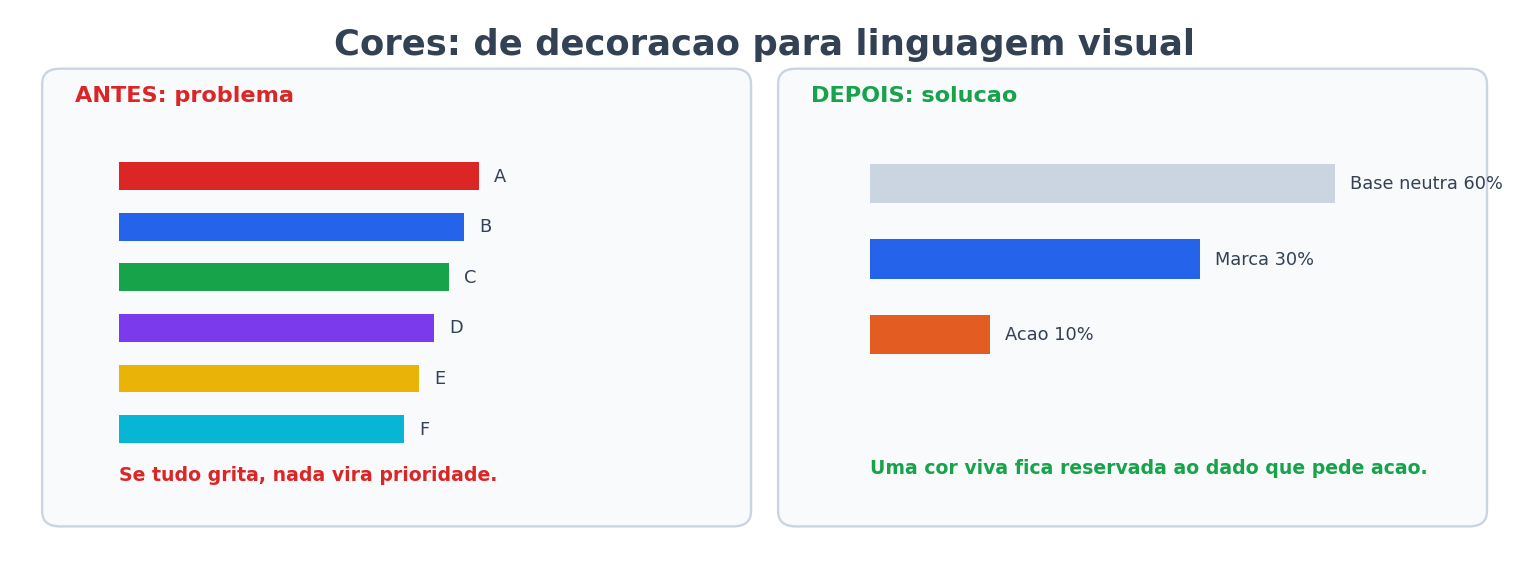
\includegraphics[width=0.58\textwidth]{semana_especial/outputs/cmp_cap1_cores.png}
\caption{Paleta de referência para dashboards. Cada cor tem uma função semântica única. Gráfico gerado pelo script \texttt{auto\_eda\_demo.py}.}
\end{figure}

\begin{BoardBox}[title=Paleta de 8 Funções --- Referência Rápida]
\begin{tabular}{@{}p{0.25cm}lll@{}}
\toprule
& \textbf{Hex} & \textbf{Função} & \textbf{Quando usar} \\
\midrule
\colorbox{colDestaque}{\phantom{M}} & \texttt{\#E35D22} & Destaque / ação urgente & O dado mais importante do dashboard \\
\colorbox{colPrimaria}{\phantom{M}} & \texttt{\#2563EB} & Primária / navegação    & Barras de base, links, filtros \\
\colorbox{colPositivo}{\phantom{M}} & \texttt{\#16A34A} & Positivo / meta atingida & Setas de alta, gaps positivos, badges OK \\
\colorbox{colAlerta}{\phantom{M}}   & \texttt{\#DC2626} & Alerta / falha / risco  & Abaixo da meta, KPI crítico \\
\colorbox{colAtencao}{\phantom{M}}  & \texttt{\#EAB308} & Atenção / monitorar     & Perto do limite, 80--99\% da meta \\
\colorbox{colNeutra}{\phantom{M}}   & \texttt{\#64748B} & Neutra / base           & Eixos, grades, texto secundário \\
\colorbox{colMarca}{\phantom{M}}    & \texttt{\#0B3D2E} & Marca / fundo escuro    & Header, rodapé, modo dark \\
\colorbox{colBgClaro}{\phantom{M}}  & \texttt{\#E2E8F0} & Background / fundo      & Área de trabalho do dashboard \\
\bottomrule
\end{tabular}
\end{BoardBox}

\paragraph{Acessibilidade e daltonismo.}
8\% dos homens e 0,5\% das mulheres têm alguma forma de daltonismo. O tipo mais comum é o deuteranopia (vermelho--verde). Regras práticas: (1) nunca use vermelho e verde como únicos diferenciadores --- adicione ícone de alta/baixa ou rótulo de texto; (2) use ferramentas como \textit{Color Oracle} ou \textit{Coblis} para simular; (3) o par azul--laranja tem alto contraste para daltonismo vermelho--verde e é a combinação padrão de grande parte dos dashboards corporativos.

\paragraph{Cor no Tableau e no QuickSight.}
No Tableau: \texttt{Format} $\to$ \texttt{Color} $\to$ \texttt{Edit Colors} define a paleta da view; use \texttt{Custom Diverging} para heatmaps; use \texttt{Single Color} com opacidade para barras onde o comprimento é o dado. No QuickSight: paletas são definidas no \textit{Theme JSON} e aplicadas globalmente no dataset; campos calculados com `ifelse` podem forçar cor semântica por condição.

% =============================================================
\section{Caminho do Olhar: Analista, Gerente e CEO}
\label{sec:olhar}
% =============================================================

Cada perfil de leitor olha para um dashboard em uma ordem diferente. Ignorar isso é o motivo pelo qual dashboards perfeitamente analíticos falham na sala de board. Entender o caminho do olhar de cada perfil é tão importante quanto escolher o gráfico certo.

\paragraph{O padrão F (analista).}
Pesquisas de eye-tracking de Jakob Nielsen (2006, \textit{Eyetracking Web Usability}) mostram que leitores técnicos percorrem o conteúdo em um padrão em forma de F: (1) leem a linha superior completa; (2) voltam ao início e leem a segunda linha; (3) varrem verticalmente o lado esquerdo em busca de palavras-chave. Implicação para dashboards: \textbf{coloque os dados mais importantes na primeira linha e no canto superior esquerdo}. O analista vai ler tudo, mas a ordem vai moldar o que ele interpreta como importante.

\paragraph{O padrão Z (executivo).}
O executivo com 5 minutos por dia varre o dashboard em Z: canto superior esquerdo $\to$ canto superior direito $\to$ diagonal $\to$ canto inferior esquerdo $\to$ canto inferior direito. Implicação: \textbf{Big Number + título-mensagem no topo esquerdo; Call to Action no rodapé direito; gráfico mais importante na diagonal}.

\begin{BoardBox}[title=Layout em Z para Dashboard Executivo]
\begin{verbatim}
[BIG NUMBER + Big Idea]  ->  [KPI2 | KPI3]
        diagonal
[Grafico diagnostico]    ->  [CALL TO ACTION]
\end{verbatim}
Percurso: (1) KPI principal com delta vs meta; (2) título-mensagem já conta a história;
(3) gráfico de diagnóstico para quem quer o detalhe; (4) CTA com verbo + prazo.
\end{BoardBox}

\begin{figure}[H]
\centering
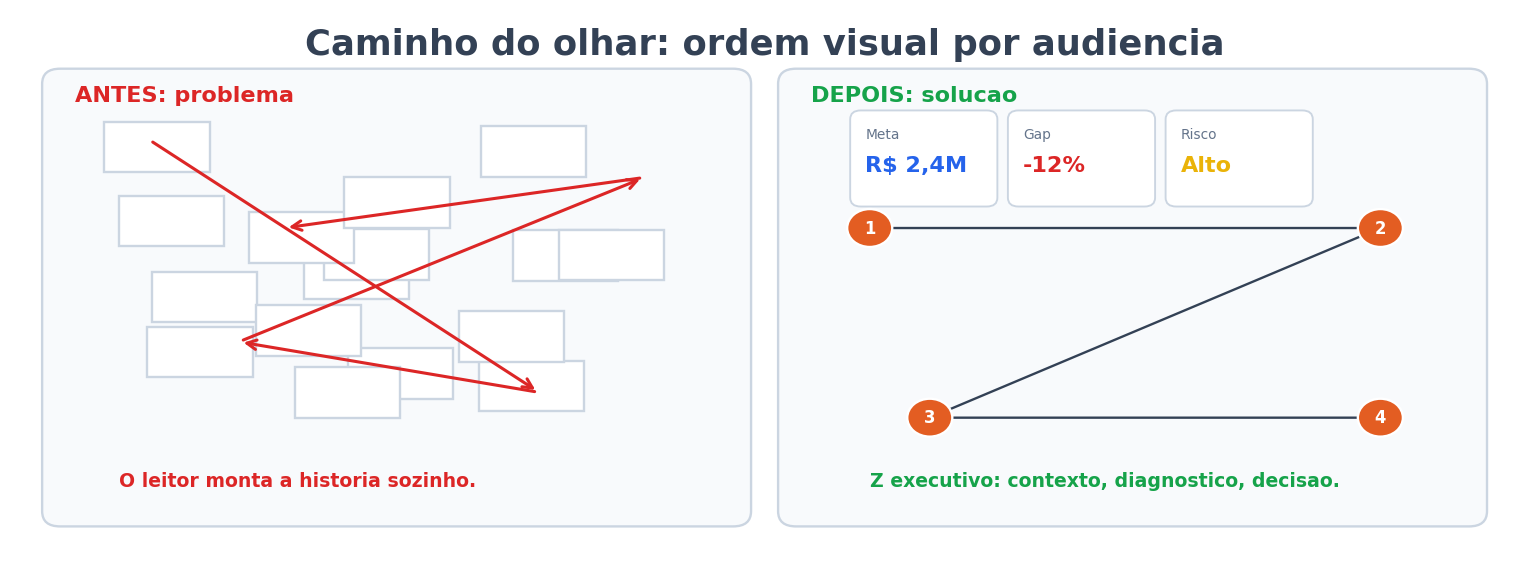
\includegraphics[width=0.58\textwidth]{semana_especial/outputs/cmp_cap1_olhar.png}
\caption{Caminho do olhar por perfil. Use esta figura em aula para mostrar que o mesmo dashboard pode falhar se a ordem visual não combinar com a audiência: o analista lê em F, o executivo varre em Z, e o gerente procura KPI, exceção e tabela de detalhe.}
\end{figure}

\paragraph{Perfil CEO: scanning semântico.}
O CEO não lê gráficos --- ele lê \emph{títulos}. Se os 4 títulos do dashboard entregam as mensagens, o CEO tomou a decisão antes de olhar qualquer eixo. A regra prática: todos os títulos de gráficos em linguagem de manchete de jornal. ``Gráfico de Barras'' $\to$ não. ``Sul lidera com 2,4$\times$ a média'' $\to$ sim.

\paragraph{Perfil gerente/gestor: diagonal + tabela.}
O gerente quer confirmar a hipótese que já tem. Ele vai direto ao gráfico que trata do seu KPI, verifica se o número confirma o que sente, e depois olha a tabela analítica no rodapé para entender as exceções. Implicação: \textbf{ofereça sempre uma tabela de detalhe no rodapé} --- ela não polui o design (ocupa a parte inferior que o executivo ignora) mas salva o gerente de tomar uma decisão com dado incompleto.

\paragraph{Perfil analista: leitura completa em espiral.}
O analista começa no Big Number, vai para o scatter, tenta reproduzir o cálculo, encontra a nota metodológica, cruza com a tabela, e só então forma uma opinião. Para esse perfil, inclua: (1) definição de todas as métricas em tooltip ou nota de rodapé; (2) período de referência explícito; (3) fonte dos dados.

% =============================================================
\section{Carga Cognitiva e Dashboard Cognitivo}
\label{sec:cognitivo}
% =============================================================

A \textbf{teoria da carga cognitiva} (Sweller, 1988) distingue três tipos de carga mental que afetam a absorção de informação. Entender isso explica por que dashboards muito elaborados technicamente falham na comunicação.

\begin{BoardBox}[title=Os 3 Tipos de Carga Cognitiva]
\begin{enumerate}
  \item \textbf{Carga intrínseca:} complexidade inerente ao conteúdo (o dado em si é complicado? a análise exige raciocínio?). Você não pode reduzir isso sem simplificar a análise.
  \item \textbf{Carga extrínseca (extraneous):} esforço causado pelo design ruim. Legenda separada que exige desvio do olhar; cores sem propósito que forçam decodificação; texto e gráfico contradizendo-se. Isso é \textbf{eliminável} com bom design.
  \item \textbf{Carga germane (útil):} esforço que forma aprendizado e schema mental. É o que sobra quando você elimina a carga extrínseca. Você quer maximizar isso.
\end{enumerate}
\smallskip
\textbf{Objetivo do bom design:} eliminar toda a carga extrínseca para liberar capacidade cognitiva para a carga útil.
\end{BoardBox}

\paragraph{Princípios de Gestalt aplicados a dashboards.}
A psicologia da Gestalt descreve como o cérebro organiza elementos visuais em padrões. Cinco princípios diretos:

\begin{BoardBox}[title=Gestalt em Dashboards]
\begin{tabular}{@{}lp{4.2cm}p{5.8cm}@{}}
\toprule
\textbf{Princípio} & \textbf{O que significa} & \textbf{Aplicação prática} \\
\midrule
Proximidade   & Elementos próximos parecem relacionados  & KPIs do mesmo tema agrupados com espaço em branco entre grupos \\
Similaridade  & Elementos parecidos parecem relacionados & Mesma cor = mesma categoria; mesmo formato = mesma hierarquia \\
Fechamento    & O cérebro completa formas incompletas    & Enclosure (caixa) ao redor de KPIs = grupo implícito sem linha pesada \\
Continuidade  & O olho segue linhas e padrões de fluxo  & Gráfico de linhas sugere tendência; use linhas de referência \\
Figura-fundo  & Um elemento se destaca, o resto recua   & 1 cor de destaque em fundo cinza é pura figura-fundo \\
\bottomrule
\end{tabular}
\end{BoardBox}

\paragraph{Dashboard cognitivo: definição.}
Um dashboard cognitivo (termo popularizado por Stephen Few em \textit{Show Me the Numbers}, 2012) é aquele que foi projetado para \emph{minimizar a carga extrínseca e maximizar a carga germane}: título-mensagem que já entrega o insight; cor de destaque que guia o olho; hierarquia visual clara (importante grande, secundário pequeno); remoção de todo chartjunk; e estrutura narrativa que replica o processo de decisão da audiência-alvo.

\begin{figure}[H]
\centering
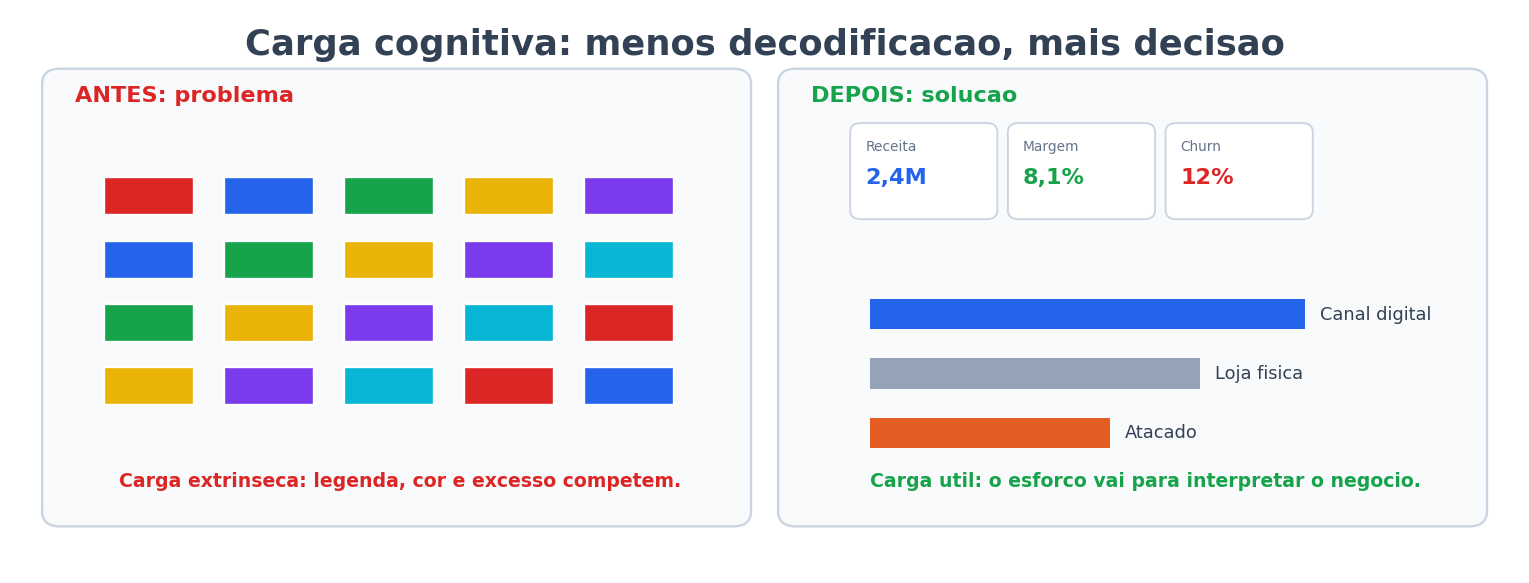
\includegraphics[width=0.58\textwidth]{semana_especial/outputs/cmp_cap1_carga.png}
\caption{Carga cognitiva aplicada a dashboards. À esquerda, o leitor gasta energia decodificando cores, formas e excesso de gráficos; à direita, a energia mental é transferida para entender o problema e decidir.}
\end{figure}

\paragraph{Número mágico 7 ± 2.}
George Miller (1956) demonstrou que a memória de trabalho humana processa 7 (mais ou menos 2) objetos simultâneos. Para dashboards: máximo de 7 KPIs na tela inicial; máximo de 7 categorias por gráfico (agrupe o restante em ``Outros''); máximo de 7 cores distintas numa paleta. Acima desses limites, a interpretação falha mesmo com dados corretos.

% =============================================================
\section{Insights Informativos}
\label{sec:insight_info}
% =============================================================

Um insight informativo é uma observação extraída dos dados que \textbf{aumenta o entendimento} de uma situação mas \emph{não orienta uma ação específica e imediata}. Ele tem valor: reduz incerteza, confirma hipóteses, fornece contexto. O problema começa quando o analista entrega \emph{apenas} insights informativos numa reunião executiva --- porque executivos não precisam de mais informação, precisam de mais clareza sobre o que fazer.

\begin{BoardBox}[title=Características de um Insight Informativo]
\begin{enumerate}
  \item \textbf{Descreve um padrão real:} algo que estava oculto nos dados e que a audiência não sabia.
  \item \textbf{É factual e verificável:} pode ser reproduzido com os mesmos dados.
  \item \textbf{Não tem urgência intrínseca:} ``interessante, mas e daí?'' é a reação esperada.
  \item \textbf{Serve de base para insights acionáveis:} todo bom insight acionável parte de um informativo.
\end{enumerate}
\end{BoardBox}

\textbf{Exemplos de insights informativos:}

\begin{itemize}
  \item ``A distribuição de Exam\_Score é aproximadamente normal (média 67,2; DP 3,9), o que indica que o dataset não tem viés de seleção severo.''
  \item ``Frequência (Attendance) tem a maior correlação com a nota final ($r = 0{,}58$), acima de horas de estudo ($r = 0{,}45$).''
  \item ``Clientes do segmento Premium têm ticket médio 3,2$\times$ maior que o segmento Standard.''
  \item ``O churn em janeiro de 2025 foi 12\% --- o maior dos últimos 24 meses.''
\end{itemize}

Insights informativos são valiosos em relatórios de EDA, em apresentações para times técnicos e em bases de conhecimento internas. O erro é confundi-los com o produto final de uma análise para a diretoria.

\begin{figure}[H]
\centering
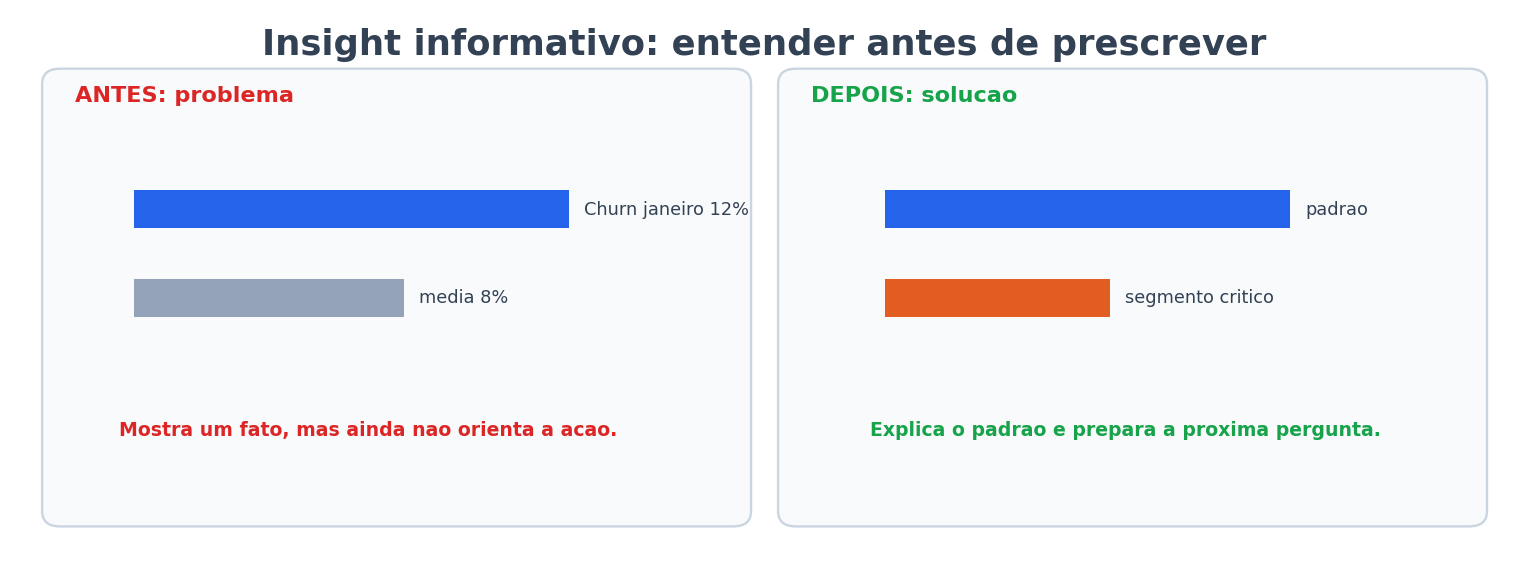
\includegraphics[width=0.58\textwidth]{semana_especial/outputs/cmp_cap1_insight_info.png}
\caption{Insight informativo em dashboard. Ele melhora o entendimento, mas ainda deixa perguntas executivas em aberto: gravidade, responsável, ação e impacto.}
\end{figure}

% =============================================================
\section{Insights Acionáveis: Do Dado à Decisão}
\label{sec:insight_acion}
% =============================================================

Este é o tópico central de qualquer analista que trabalha para a tomada de decisão. Um insight acionável \textbf{prescreve uma ação específica, direcionada a um responsável, com estimativa de impacto e prazo}. Ele não descreve o passado --- ele orienta o futuro. A diferença entre analistas júnior e sênior, na prática bancária e em qualquer grande corporação, é exatamente a capacidade de transformar observações numéricas em recomendações que mudam o comportamento de alguém.

\begin{BoardBox}[title=Fórmula do Insight Acionável --- 5 Componentes]
\begin{enumerate}
  \item \textbf{Observação:} padrão não-óbvio extraído dos dados.
  \item \textbf{Evidência:} o dado que sustenta a observação (com magnitude e significância).
  \item \textbf{Causa raiz (quando possível):} por que isso está acontecendo?
  \item \textbf{Ação prescrita:} verbo + objeto + quantidade + canal.
  \item \textbf{Impacto estimado:} resultado esperado em métrica de negócio + prazo.
\end{enumerate}
\smallskip
\textbf{Template:} ``[Observação] porque [evidência]. Se [ação prescrita] então [impacto estimado] em [prazo], responsável: [stakeholder].''
\end{BoardBox}

\paragraph{Por que a maioria dos analistas não consegue fazer isso.}
O bloqueio é conceitual: o analista foi treinado para \emph{descrever} dados, não para \emph{prescrever} ações. Descrever é seguro --- ninguém erra ao reportar que ``as vendas caíram 8\%''. Prescrever exige entender o negócio, assumir uma hipótese causal e aceitar que pode estar errado. O sênior aceita esse risco porque o valor gerado pela ação certa supera muito o custo de estar errado em uma recomendação específica.

\paragraph{Exemplos completos --- 8 domínios.}

Os exemplos a seguir seguem a estrutura de 5 componentes. Leia devagar: a diferença entre o insight informativo (coluna ``sem ação'') e o acionável (coluna ``com ação'') é a diferença de impacto na carreira de um analista.

\medskip
\textbf{Exemplo 1 --- Banco: análise de churn de cartão de crédito}

\textit{Informativo:} ``Clientes com menos de 20 transações por ano têm taxa de churn de 38\%, vs 6\% para clientes com mais de 50 transações.''

\textit{Acionável:} ``Clientes com frequência de uso $<$ 20 trans/ano e saldo médio $<$ R\$2k têm 38\% de probabilidade de cancelamento --- 3,4 pp acima da base. Acionar campanha de reengajamento personalizado via app (cashback + limite temporário) para os 8.200 clientes nesse perfil pode reverter 30\% do churn projetado, preservando R\$1,4M em receita de juros e anuidade nos próximos 12 meses. Responsável: Gerência de CRM. Prazo de implementação: 3 semanas.''

\medskip
\textbf{Exemplo 2 --- Varejo: pricing de produto}

\textit{Informativo:} ``Produtos com desconto $>$ 20\% têm margem média de $-4\%$.''

\textit{Acionável:} ``Descontos acima de 20\% em Linha Branca na Região Sul destroem R\$120k de margem por trimestre sem aumentar o volume de unidades (elasticidade próxima de zero na análise de regressão). Capear o desconto máximo em 12\% mantém a competitividade de preço percebida e projeta recuperação de R\$85k de margem trimestral. Responsável: Gerência Comercial Sul. Prazo: implementar na campanha de inverno (início de julho).''

\medskip
\textbf{Exemplo 3 --- RH: turnover de TI}

\textit{Informativo:} ``O departamento de TI tem turnover de 28\%, acima da média corporativa de 12\%.''

\textit{Acionável:} ``Engenheiros de TI com menos de 2 anos de empresa e sem promoção nos últimos 36 meses têm 3$\times$ mais probabilidade de saída que a média (28\% vs 9\%). Esse perfil representa 41 funcionários. Implantar programa de mentoria acelerada + revisão de faixa salarial para esse grupo específico pode reduzir o turnover de 28\% para 15\%, economizando R\$270k/ano em custo de reposição (R\$18k/funcionário $\times$ 15 saídas evitadas). Responsável: HRBP de TI + Diretor de Engenharia. Prazo: começar em 30 dias para impactar a janela de avaliação semestral.''

\medskip
\textbf{Exemplo 4 --- Saúde: readmissão hospitalar}

\textit{Informativo:} ``Pacientes com diabetes + hipertensão têm taxa de readmissão em 30 dias de 34\%.''

\textit{Acionável:} ``Pacientes diabéticos com HbA1c $>$ 9 e diagnóstico de HAS que receberam alta sem consulta de retorno agendada têm 34\% de readmissão em 30 dias vs 8\% quando o retorno está agendado. Implementar protocolo de agendamento obrigatório na alta para os 1.200 pacientes nesse perfil anual pode evitar 312 readmissões, economizando R\$3,7M (R\$12k/internação), além de melhorar o indicador de qualidade AHRQ-PSI. Responsável: Gerência de Assistência. Prazo: protocolo ativo no próximo semestre.''

\medskip
\textbf{Exemplo 5 --- E-commerce: logística}

\textit{Informativo:} ``O estado do Amazonas tem atraso médio de 4,7 dias acima da estimativa.''

\textit{Acionável:} ``Pedidos de Eletrônicos em AM com prazo estimado $<$ 7 dias chegam em média 4,7 dias atrasados, gerando review médio de 2,8 estrelas e taxa de devolução 18\% acima da média. Substituir a transportadora atual por operador regional com SLA de 5 dias para essa rota reduz o atraso estimado em 70\%, projeta melhora do review para 4,1 estrelas e reduz devoluções em R\$95k/semestre. Responsável: Gerência de Logística. Prazo: RFP para transportadora em 45 dias.''

\medskip
\textbf{Exemplo 6 --- Fintech: crédito}

\textit{Informativo:} ``A inadimplência de empréstimo pessoal cresceu 3 pp em Q1/2026.''

\textit{Acionável:} ``Clientes de empréstimo pessoal com renda variável (profissional autônomo) que acessaram o produto em fevereiro/março têm inadimplência de 19\%, contra 7\% para clientes com renda fixa. O crescimento de 3 pp na inadimplência total é explicado em 78\% por esse segmento (análise de decomposição). Ajustar a política de crédito para limitar o LTV de empréstimo pessoal a 60\% da renda variável comprovada pode reduzir a inadimplência desse perfil de 19\% para 10\%, preservando R\$4,2M em provisão de crédito no próximo trimestre. Responsável: Gerência de Risco de Crédito. Prazo: vigência imediata para novas contratações.''

\medskip
\textbf{Exemplo 7 --- Educação (dataset StudentPerformance)}

\textit{Informativo:} ``Frequência (Attendance) tem correlação de 0,58 com Exam\_Score, sendo o preditor mais forte entre as variáveis numéricas.''

\textit{Acionável:} ``Alunos com frequência $<$ 75\% nos meses de março--abril têm nota final média 9,3 pts abaixo da média geral (67,2), e 34\% deles reprovam. Implementar sistema de alerta automático por WhatsApp para responsáveis quando o aluno atingir 3 faltas consecutivas pode recuperar 40\% desses alunos (baseado em piloto de 2024), reduzindo a taxa de reprovação de 8\% para 4,8\%, equivalendo a 216 alunos aprovados adicionais por semestre. Responsável: Coordenação Pedagógica + TI. Prazo: sistema ativo no início do semestre seguinte.''

\medskip
\textbf{Exemplo 8 --- Marketing digital: aquisição}

\textit{Informativo:} ``O CAC médio pelo canal Google Ads é R\$48, contra R\$31 pelo canal Organic.''

\textit{Acionável:} ``O canal Google Ads tem CAC 55\% maior que o orgânico, mas o LTV dos clientes adquiridos por Google Ads é apenas 8\% maior (R\$320 vs R\$296). O ROI ajustado ao LTV do canal pago é negativo ($-$4\%) no primeiro ano. Redirecionar 40\% do orçamento de Google Ads para SEO/Content durante 6 meses projeta redução do CAC médio de R\$48 para R\$35, com impacto de $-$12\% no volume de aquisição no curto prazo mas retorno positivo a partir do mês 8. Responsável: Gerência de Marketing. Prazo: próximo ciclo de orçamento (Q3 2026).''

\paragraph{Como treinar a habilidade de gerar insights acionáveis.}
O caminho mais rápido é forçar a pergunta ``\emph{e daí?}'' sobre cada dado encontrado. Toda vez que você escrever uma observação, pergunte: ``E daí?'' até chegar num verbo de ação ligado a um responsável. Veja a cadeia:

\begin{BoardBox}[title=A Cadeia ``E Daí?'' --- Exercício Prático]
\textbf{Observação inicial:} ``O churn subiu 3\%.'' \quad \textbf{E daí?}\\
\textbf{Nível 2:} ``Clientes do segmento X estão cancelando mais.'' \quad \textbf{E daí?}\\
\textbf{Nível 3:} ``Clientes do segmento X com produto Y cancelam 4$\times$ mais no 3$^\circ$ mês.'' \quad \textbf{E daí?}\\
\textbf{Nível 4:} ``O problema é que o onboarding do produto Y não é completado por 60\% dos clientes.'' \quad \textbf{E daí?}\\
\textbf{Insight acionável:} ``Criar fluxo de onboarding guiado no app para produto Y, com nudge no dia 15, pode reduzir o churn do segmento X de 18\% para 8\%, preservando R\$XX em ARR. Responsável: PM + CRM. Prazo: 4 semanas.''
\end{BoardBox}

\begin{figure}[H]
\centering
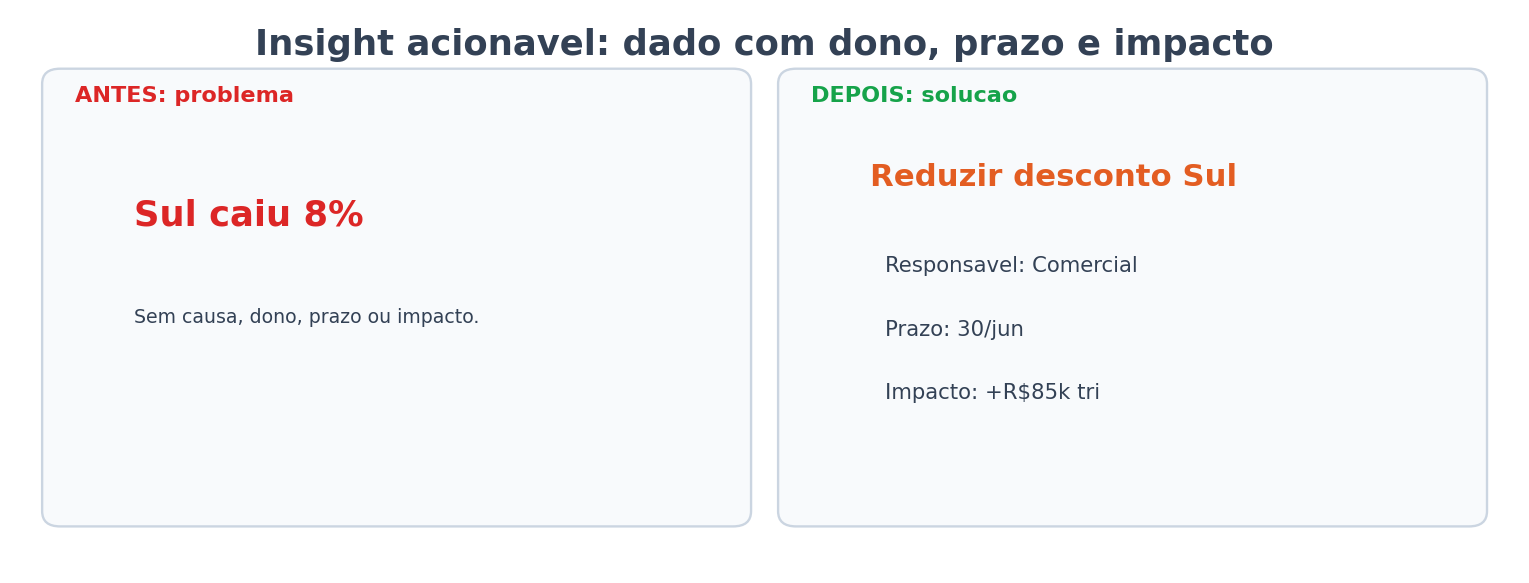
\includegraphics[width=0.58\textwidth]{semana_especial/outputs/cmp_cap1_insight_acionavel.png}
\caption{Dashboard sem ação versus dashboard com insight acionável. O segundo não apenas descreve o problema: ele explicita o que fazer, quem deve fazer, até quando e qual impacto esperado.}
\end{figure}

% =============================================================
\section{Dashboard as Code: AWS e QuickSight}
\label{sec:daac}
% =============================================================

\textbf{Dashboard as Code (DaC)} é a prática de definir, versionar e publicar dashboards inteiramente via código e infraestrutura como código (IaC), eliminando configuração manual via interface gráfica. Os benefícios diretos para um time de analytics bancário são: rastreabilidade via Git, reprodutibilidade entre ambientes (dev/homol/prod), revisão de mudanças por Pull Request, e orquestração programática de dezenas de dashboards.

\paragraph{AWS QuickSight e as APIs de criação.}
O QuickSight expõe uma API REST completa (\textit{aws quicksight} via Boto3 ou CLI) que permite criar e atualizar todos os recursos: datasets, análises, dashboards e permissões. Os objetos principais na hierarquia são:

\begin{BoardBox}[title=Hierarquia de Objetos no QuickSight]
\begin{tabular}{@{}llp{6.5cm}@{}}
\toprule
\textbf{Objeto} & \textbf{API} & \textbf{Descrição} \\
\midrule
DataSource    & \texttt{create-data-source}    & Conexão ao S3/Redshift/Athena/RDS \\
DataSet       & \texttt{create-data-set}       & Schema, joins, campos calculados, filtros de linha \\
Analysis      & \texttt{create-analysis}       & Canvas de edição (não publicado) \\
Dashboard     & \texttt{create-dashboard}      & Versão publicada de uma Analysis \\
Template      & \texttt{create-template}       & Snapshot de uma Analysis reutilizável cross-account \\
Theme         & \texttt{create-theme}          & Paleta de cores, fontes e layout globais \\
\bottomrule
\end{tabular}
\end{BoardBox}

\paragraph{Fluxo conceitual do Dashboard as Code.}
Para esta aula, o importante não é decorar código de Boto3 ou CDK. O ponto central é entender que o dashboard deixa de ser uma peça manual feita no clique e passa a ser um artefato governado: nasce de uma regra de negócio, é versionado, revisado, homologado e publicado com rastreabilidade.

\begin{figure}[H]
\centering
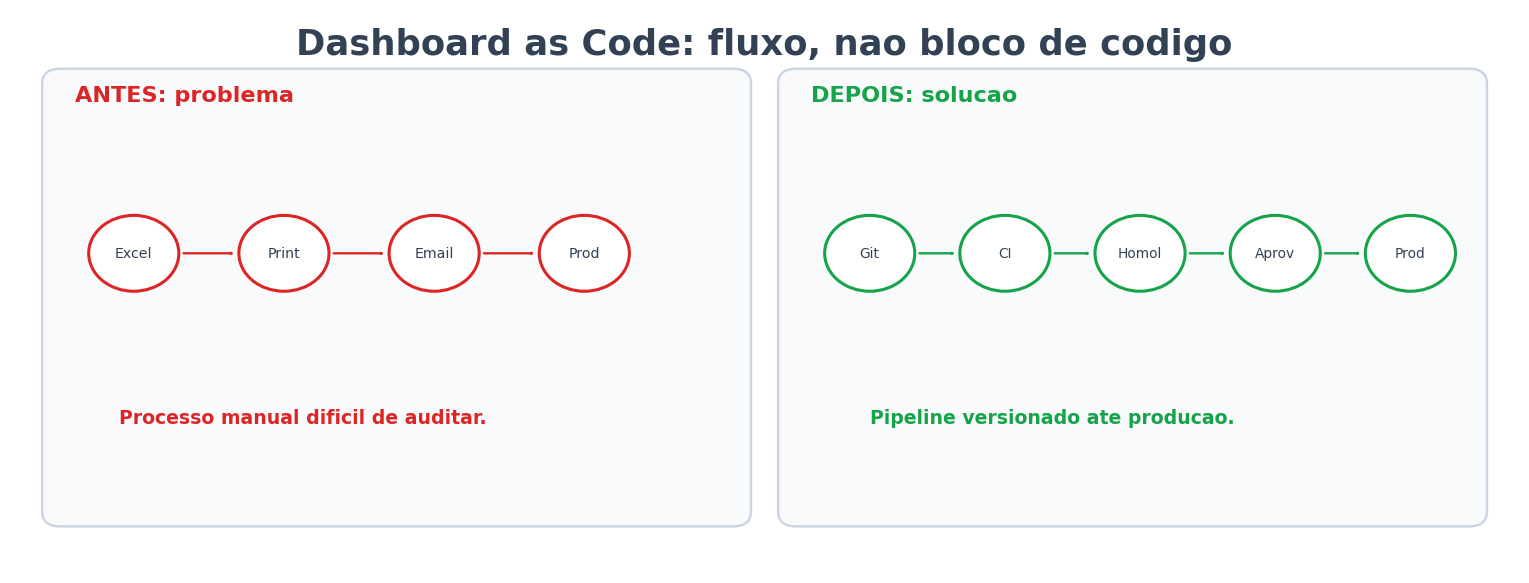
\includegraphics[width=0.58\textwidth]{semana_especial/outputs/cmp_cap1_dac.png}
\caption{Fluxo conceitual de Dashboard as Code. A criação programática só faz sentido quando protege governança: regra de negócio clara, definição versionada, revisão por pares, homologação e publicação controlada.}
\end{figure}

\paragraph{Fluxo de trabalho DaC com Git.}
O padrão recomendado para times de analytics em bancos: (1) \texttt{feature/dashboard-churn} branch; (2) código Python com definição de datasets + análise em JSON (exportado via \texttt{describe-analysis-definition}); (3) PR com revisão de outro analista; (4) merge em \texttt{main} dispara GitHub Actions que chama \texttt{boto3.update\_dashboard}; (5) tags de versão correspondem a versões do QuickSight.

\paragraph{Asset Bundle Export/Import.}
Para migração entre contas (dev $\to$ prod) sem recriar tudo manualmente, o QuickSight oferece desde 2023 o \textbf{Asset Bundle} API: exporta análises, dashboards, datasets e temas em JSON e importa em outra conta com substituição de ARNs. Isso é o equivalente ao \texttt{terraform plan/apply} para dashboards.

% =============================================================
\section{AED Automática: Bibliotecas, Relatórios e Interpretação}
\label{sec:autoeda}
% =============================================================

As bibliotecas de AED automática (profiling) fazem em uma linha o que levaria horas de código manual: calculam estatísticas descritivas, detectam outliers, mapeiam correlações, identificam dados ausentes, avaliam distribuições e geram relatório HTML completo. Elas não substituem a análise --- substituem a parte mecânica para que o analista foque na interpretação.

\begin{BoardBox}[title=Principais Bibliotecas de AED Automática (Python)]
\begin{tabular}{@{}lp{3.5cm}p{5.8cm}@{}}
\toprule
\textbf{Biblioteca} & \textbf{Melhor para} & \textbf{Diferencial} \\
\midrule
\texttt{ydata-profiling} & Relatório completo solo & 1 linha; HTML interativo; detecta correlações, outliers, duplicatas, alertas de qualidade \\
\texttt{sweetviz}        & Comparação de grupos    & Visualiza diferenças entre treino/teste ou segmentos lado a lado; target analysis \\
\texttt{autoviz}         & Visualizações rápidas   & Gera gráficos automaticamente sem HTML; bom para exploração rápida \\
\texttt{D-Tale}          & Exploração interativa   & Interface web local tipo Excel interativo; edição de dados em tempo real \\
\texttt{lux}             & Recomendação automática & Sugere visuais relevantes contextualizados ao DataFrame; integra Jupyter \\
\bottomrule
\end{tabular}
\end{BoardBox}

\paragraph{Como ler um relatório automático.}
Nesta aula, não precisamos decorar comandos. O que importa é saber interpretar o HTML produzido por essas ferramentas. Primeiro olhe os \textbf{alertas de qualidade}: dados ausentes, duplicatas, cardinalidade alta e colunas constantes. Depois leia as \textbf{distribuições}: assimetria, outliers e concentração. Em seguida, veja \textbf{correlações e associações}: elas sugerem hipóteses, mas não provam causalidade. Por fim, transforme o relatório em perguntas de negócio: ``qual variável explica o resultado?'', ``qual grupo merece intervenção?'', ``que dado precisa ser validado antes da decisão?''.

\begin{figure}[H]
\centering
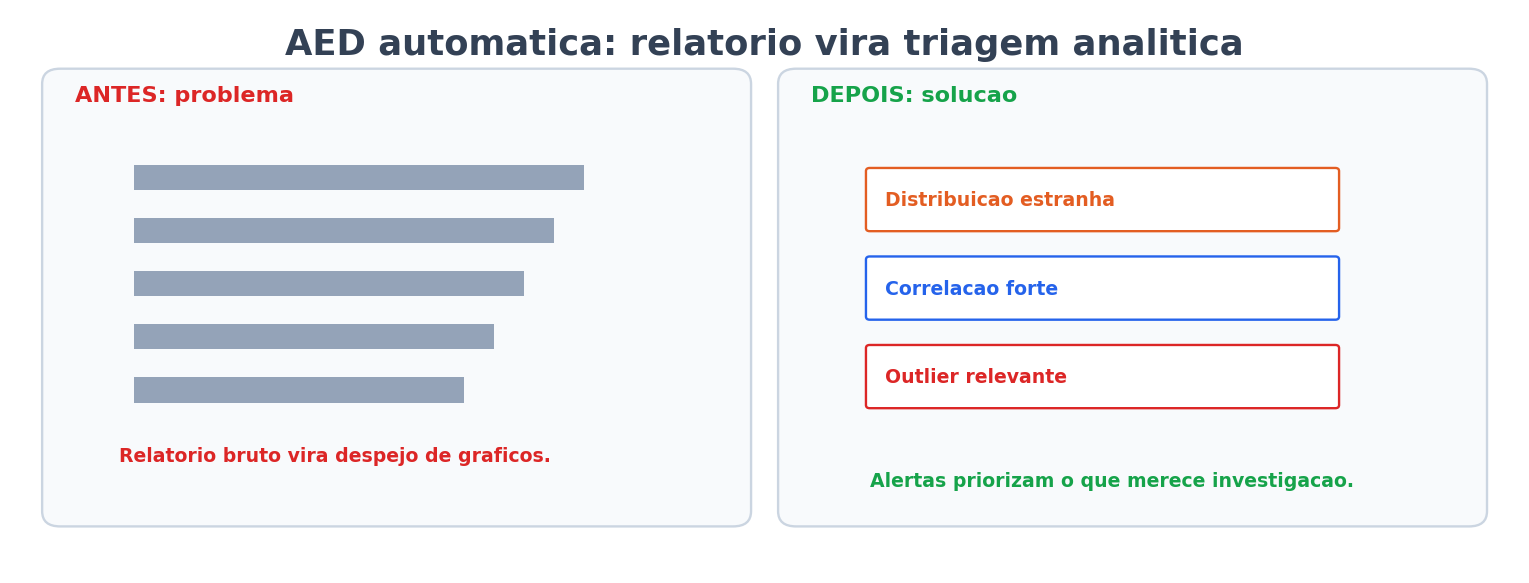
\includegraphics[width=0.58\textwidth]{semana_especial/outputs/cmp_cap1_autoeda.png}
\caption{Fluxo de leitura da AED automática. O HTML é um ponto de partida: ele encontra sinais, mas o analista precisa explicar o significado e formular a próxima pergunta.}
\end{figure}

\paragraph{Exemplo real: StudentPerformanceFactors.csv.}

Rodamos \texttt{ydata-profiling} (modo minimal, 6607 registros, 20 variáveis) e \texttt{sweetviz} no dataset deste curso. Os relatórios HTML estão em \texttt{semana\_especial/outputs/}:
\begin{itemize}
  \item \texttt{ydata\_profiling\_report.html} --- perfil completo com alertas de qualidade, correlações, distribuições
  \item \texttt{sweetviz\_report.html} --- target analysis com Exam\_Score como variável alvo
\end{itemize}

Em aula, use esses relatórios como material de inspeção: eles mostram distribuições, correlações, scatterplots e variáveis categóricas. O PDF mantém apenas o comparativo acima para não repetir quatro figuras exploratórias onde uma síntese visual resolve melhor.

\paragraph{Alertas automáticos que o ydata-profiling detecta.}
O relatório HTML sinaliza automaticamente: variáveis com $>$ 5\% de dados ausentes; colunas com alta correlação ($>$ 0,9) que indicam redundância; variáveis com cardinalidade muito alta (suspeita de ID); distribuições muito assimétricas (candidatas a transformação log); valores constantes ou quase-constantes.

\paragraph{Quando NÃO usar AED automática.}
Quando o dataset tem $>$ 10M de linhas (o relatório trava ou demora demais --- use uma amostra estratificada de 50k--100k linhas); quando as variáveis têm semântica muito específica do negócio que a biblioteca não conhece (ex.: códigos de agência bancária precisam de dicionário manual); quando o objetivo já é confirmatory (você já sabe o que procura --- vá direto).

% =============================================================
\section{Arquitetura de Agentes para AED e Dashboards}
\label{sec:agentes}
% =============================================================

A abordagem de agentes para análise de dados está passando de experimento acadêmico para realidade em grandes bancos e fintechs em 2025--2026. A ideia central é substituir o fluxo manual linear (analista faz EDA $\to$ analista faz perguntas $\to$ analista constrói dashboard) por um \textbf{pipeline orquestrado de agentes especializados}, cada um responsável por uma etapa e passando seu output como contexto estruturado para o próximo.

\paragraph{A arquitetura descrita.}
O pipeline que estamos construindo no banco tem a seguinte cadeia:

\begin{BoardBox}[title=Pipeline Multi-Agente --- Etapas]
\begin{enumerate}
  \item \textbf{Agente Discovery:} lê o contrato de negócio (dores, KPIs, audiência), carrega o dataset, calcula estatísticas descritivas, mapeia correlações, detecta outliers. Output: JSON com contexto estruturado.
  \item \textbf{Agente de Insights:} recebe o JSON do Agente 1, consulta a base especializada de insights (seção 9), e gera insights acionáveis candidatos com score de relevância.
  \item \textbf{Agente de Storyboard:} define Big Idea, estrutura 3 zonas (Contexto/Diagnóstico/Recomendação), monta a sequência de gráficos e os títulos-mensagem.
  \item \textbf{Agente Protótipo:} gera HTML completo do dashboard com Chart.js, auto-contido, com dados reais do dataset. Output: \texttt{prototipo.html}.
  \item \textbf{Agente de Infraestrutura (AWS):} recebe o protótipo aprovado, converte para definição QuickSight (JSON/API), cria DataSet + Analysis + Dashboard via Boto3.
  \item \textbf{Agente de Documentação:} gera changelog, dicionário de métricas e runbook automaticamente a partir dos metadados dos agentes anteriores.
\end{enumerate}
\smallskip
\textbf{Orquestrador:} LangChain / LangGraph / AWS Step Functions (para pipelines produtivos em nuvem).
\end{BoardBox}

\begin{figure}[H]
\centering
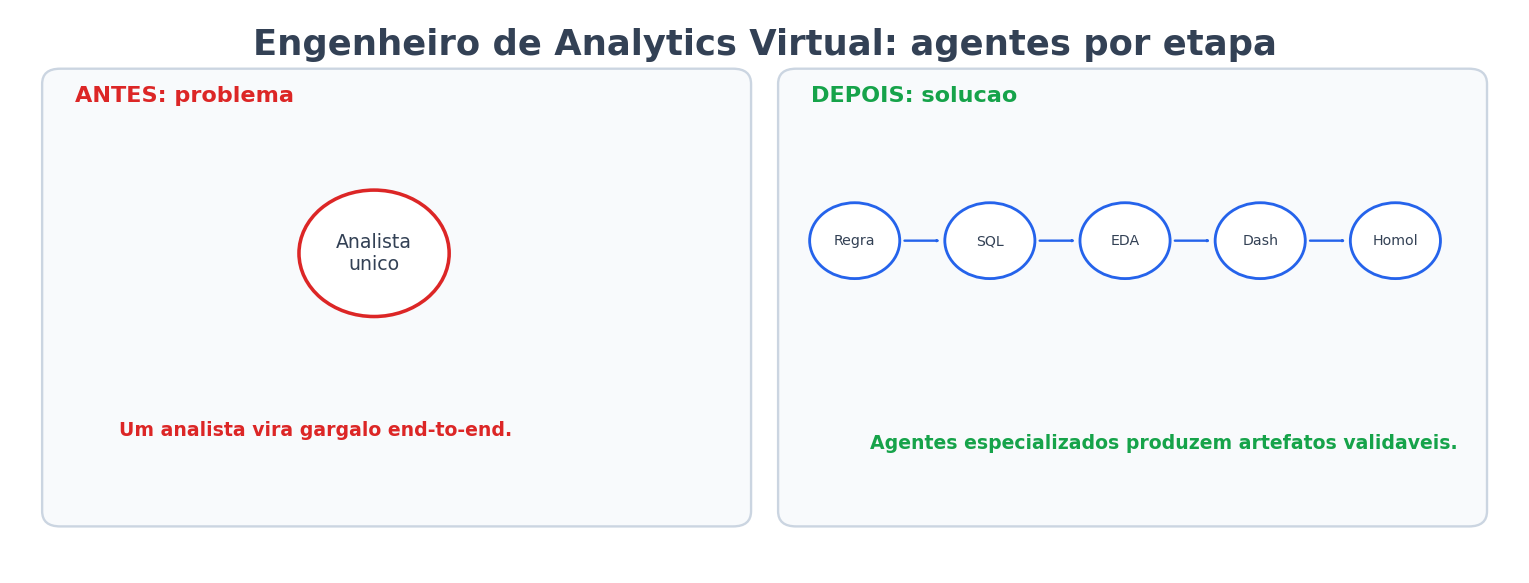
\includegraphics[width=0.58\textwidth]{semana_especial/outputs/cmp_cap1_agentes.png}
\caption{Arquitetura lúdica do Engenheiro de Analytics Virtual. A ideia prática é end-to-end: da regra de negócio até a publicação do dashboard, cada agente produz um artefato que pode ser revisado e homologado.}
\end{figure}

\paragraph{Protótipo gerado pelo pipeline.}

O script \texttt{agente\_prototipo\_html.py} executa os Agentes 1--4 localmente, sem LLM externo, usando apenas pandas e Chart.js. O arquivo \texttt{prototipo\_dashboard\_agente.html} está em \texttt{semana\_especial/outputs/}. Ele demonstra a estrutura que o pipeline mais completo (com LLM) produziria.

\paragraph{Como funcionaria na prática.}
Imagine que a área de negócio pede: ``o churn do cartão Premium subiu e precisamos decidir uma campanha''. O Agente de Negócio transforma isso em contrato: audiência, dor, métrica-alvo, restrições e prazo. O Agente de Dados valida tabelas, chaves, granularidade e qualidade. O Agente SQL cria ou sugere views analíticas. O Agente EDA procura padrões. O Agente de Insights transforma padrões em recomendações. O Agente Storyboard escolhe a sequência narrativa. O Agente Protótipo gera um HTML para homologação rápida. Só depois de aprovado entram os agentes de produção: criação de dataset, dashboard no BI, permissões, documentação e changelog.

\begin{BoardBox}[title=Artefatos por Agente]
\begin{tabular}{@{}lp{8.7cm}@{}}
\toprule
\textbf{Agente} & \textbf{Artefato entregue} \\
\midrule
Negócio & contrato de análise: dor, KPI, audiência, decisão esperada \\
Dados/SQL & tabela, view ou consulta validada com dicionário de métricas \\
EDA & resumo visual de padrões, outliers, correlações e alertas \\
Insights & 2--3 recomendações acionáveis com impacto e responsável \\
Storyboard & Big Idea, zonas do dashboard e títulos-mensagem \\
Protótipo & HTML navegável para homologação com usuário \\
Produção & dashboard publicado, permissões, documentação e versão \\
\bottomrule
\end{tabular}
\end{BoardBox}

\paragraph{Padrões de multi-agente: ReAct, Chain-of-Thought e Tool-Use.}
Três padrões são relevantes para o pipeline de analytics: (1) \textbf{ReAct} (Yao et al., 2022) --- o agente raciocina (\textit{Thought}) e então age (\textit{Action}), iterando até atingir o objetivo; ideal para o Agente de Insights que precisa testar hipóteses. (2) \textbf{Chain-of-Thought} (Wei et al., 2022) --- o agente externaliza o raciocínio passo a passo antes de entregar o output; útil no Agente de Storyboard para justificar cada decisão de layout. (3) \textbf{Tool-Use / Function-Calling} (OpenAI, 2023) --- o agente chama funções externas (Boto3, Tableau API, base de dados) de forma estruturada; é o que habilita o Agente de Infraestrutura a criar dashboards reais no QuickSight.

% =============================================================
\section{Como Criar Insights Acionáveis: Base Especializada}
\label{sec:insight_base}
% =============================================================

O maior gargalo para gerar insights acionáveis em escala (em um time de 20 analistas, para dezenas de produtos) é a \textbf{inconsistência de qualidade}. Cada analista usa sua própria definição do que é um insight, seu próprio template, sua própria escala de urgência. O resultado: 80\% dos ``insights'' entregues são observações descritivas, e os executivos param de ler relatórios de dados.

A solução é criar uma \textbf{base especializada em insights}: um repositório estruturado (tabela, vector store ou knowledge base) que contém exemplos de alta qualidade validados pelo negócio, que serve de referência para analistas humanos e de few-shot context para agentes de IA.

\begin{figure}[H]
\centering
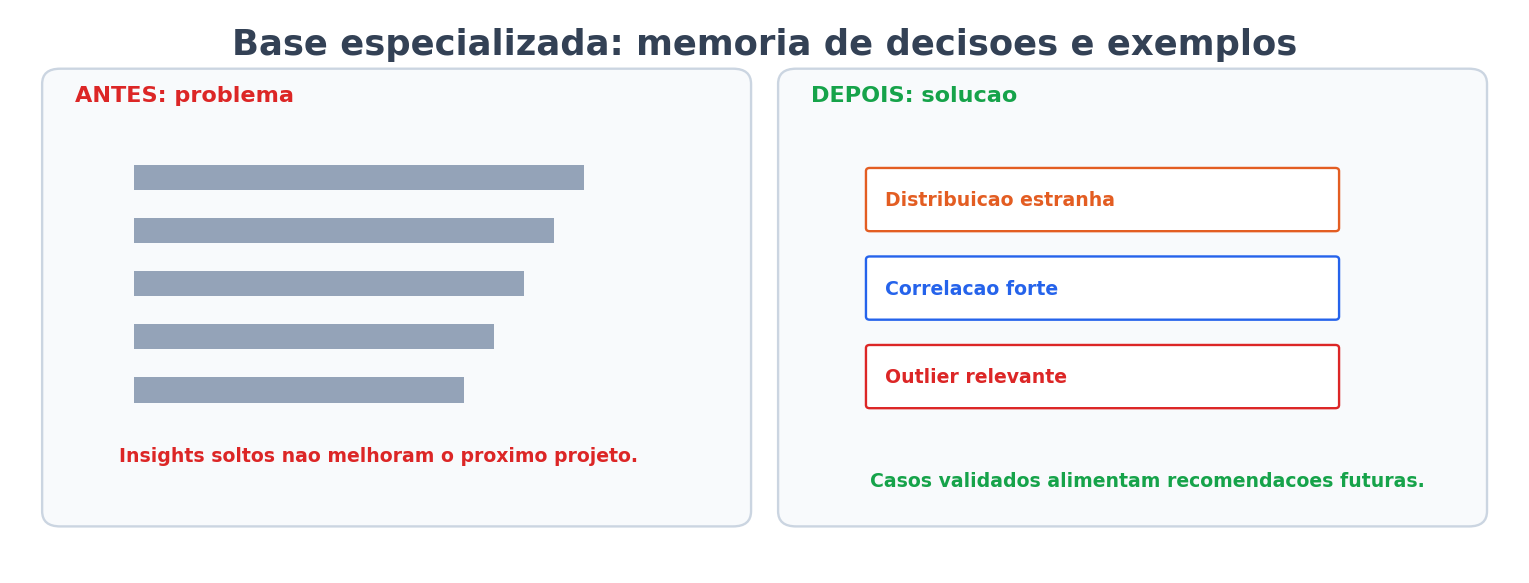
\includegraphics[width=0.58\textwidth]{semana_especial/outputs/cmp_cap1_base_insights.png}
\caption{Base especializada de insights. Ela funciona como memória de qualidade: exemplos validados alimentam novos agentes e padronizam o que a turma deve chamar de insight acionável.}
\end{figure}

\begin{BoardBox}[title=Tabela \texttt{insight\_base}]
\small
\begin{tabular}{@{}p{3.2cm}p{2.2cm}p{5.6cm}@{}}
\toprule
\textbf{Campo} & \textbf{Tipo} & \textbf{Descrição} \\
\midrule
\texttt{insight\_id}    & VARCHAR(20)  & Identificador único (ex.: INS-001) \\
\texttt{dominio}        & VARCHAR(50)  & Área do negócio (Crédito, Varejo, RH\ldots) \\
\texttt{tipo}           & ENUM         & \texttt{acionavel} | \texttt{informativo} \\
\texttt{titulo}         & VARCHAR(200) & Frase-resumo do insight (padrão + ação) \\
\texttt{observacao}     & TEXT         & Padrão detectado com dado concreto \\
\texttt{evidencia}      & TEXT         & Estatística que sustenta (n, correlação, delta) \\
\texttt{causa\_raiz}    & TEXT         & Hipótese causal (quando disponível) \\
\texttt{acao}           & TEXT         & Verbo + objeto + canal + quantidade \\
\texttt{impacto}        & TEXT         & Resultado esperado em métrica de negócio \\
\texttt{stakeholder}    & VARCHAR(100) & Responsável pela ação \\
\texttt{urgencia}       & ENUM         & \texttt{Alta} | \texttt{Media} | \texttt{Baixa} \\
\texttt{prazo\_sugerido}& VARCHAR(50)  & Ex.: ``Q3 2026'', ``próximo semestre'' \\
\texttt{fonte}          & VARCHAR(200) & Dataset / tabela de origem \\
\texttt{validado\_por}  & VARCHAR(100) & Analista ou gestor que validou o insight \\
\texttt{data\_criacao}  & DATE         & Data de geração \\
\texttt{embedding}      & VECTOR(1536) & Embedding semântico para busca por similaridade \\
\bottomrule
\end{tabular}
\end{BoardBox}

\paragraph{Exemplo real gerado pelo pipeline.}

O arquivo \texttt{insight\_base\_exemplo.csv} em \texttt{semana\_especial/outputs/} contém 3 registros gerados automaticamente pelo Agente de Insights sobre o dataset StudentPerformance. A estrutura é a mesma para qualquer domínio.

\paragraph{Como o agente usa a base para gerar novos insights.}
O Agente de Insights (seção anterior) faz o seguinte: (1) calcula as estatísticas do dataset atual (Agente 1); (2) busca na base especializada os 3--5 insights mais similares por domínio + tipo de padrão (busca vetorial por embedding semântico); (3) usa esses exemplos como \textit{few-shot context} no prompt do LLM; (4) o LLM gera um insight acionável seguindo exatamente o schema. A qualidade dos exemplos na base determina diretamente a qualidade dos insights gerados.

\begin{BoardBox}[title=Uso da Base pelo Agente]
Na prática, o agente não ``inventa'' do zero. Ele recebe o contexto do dataset, busca exemplos parecidos na base, compara o padrão atual com casos já validados, e então gera uma recomendação no mesmo formato: observação, evidência, ação, impacto, responsável e prazo. Isso reduz variação de qualidade entre analistas e evita que uma observação descritiva seja vendida como insight.
\end{BoardBox}

\paragraph{Construir a base de forma contínua.}
A base deve crescer com cada projeto: (1) analista gera insights; (2) gestor valida e adiciona o campo \texttt{validado\_por}; (3) após 6 meses, mede-se a taxa de adoção das ações recomendadas e o impacto realizado vs estimado --- isso cria um loop de melhoria contínua na qualidade dos insights gerados.

Em produção na AWS, a base pode ser: uma tabela no DynamoDB (para escrita/leitura rápida por analistas) + uma coleção no Amazon Bedrock Knowledge Base (para busca semântica pelo agente) + um bucket S3 como backup e auditoria.

% =============================================================
\section*{Referências: Cognição, Insights e Automação}
% =============================================================

As referências abaixo estão disponíveis para download e leitura. As marcadas com \textbf{[BANCO]} são particularmente relevantes para aplicação em analytics bancário.

\begin{itemize}
  \item \textbf{Few, S. (2006).} \textit{Information Dashboard Design}. O'Reilly. --- Framework de carga cognitiva aplicado a dashboards; dashboards cognitivos. \textbf{[BANCO]}

  \item \textbf{Few, S. (2012).} \textit{Show Me the Numbers} (2ª ed.). Analytics Press. --- Teoria de design de gráficos; data-ink ratio; pré-atenção.

  \item \textbf{Sweller, J. (1988).} ``Cognitive Load During Problem Solving: Effects on Learning''. \textit{Cognitive Science}, 12(2), 257--285. --- Teoria original da carga cognitiva. DOI: 10.1207/s15516709cog1202\_4

  \item \textbf{Miller, G. A. (1956).} ``The Magical Number Seven, Plus or Minus Two''. \textit{Psychological Review}, 63(2), 81--97. --- Limite de memória de trabalho; regra dos 7 KPIs. DOI: 10.1037/h0043158

  \item \textbf{Ware, C. (2004).} \textit{Information Visualization: Perception for Design} (2ª ed.). Morgan Kaufmann. --- Fundamentos neurocientíficos de visualização. \textbf{[BANCO]}

  \item \textbf{Nielsen, J. \& Pernice, K. (2010).} \textit{Eyetracking Web Usability}. New Riders. --- Padrões F e Z de leitura; eye-tracking em interfaces.

  \item \textbf{Duarte, N. (2019).} \textit{DataStory: Explain Data and Inspire Action Through Story}. Ideapress. --- Big Idea; estrutura narrativa SCR; pitch de dados.

  \item \textbf{Tufte, E. R. (1983).} \textit{The Visual Display of Quantitative Information}. Graphics Press. --- Data-ink ratio; chartjunk; small multiples.

  \item \textbf{Yao, S. et al. (2022).} ``ReAct: Synergizing Reasoning and Acting in Language Models''. \textit{arXiv:2210.03629}. --- Padrão ReAct para agentes LLM. \url{https://arxiv.org/abs/2210.03629} \textbf{[BANCO]}

  \item \textbf{Wei, J. et al. (2022).} ``Chain-of-Thought Prompting Elicits Reasoning in Large Language Models''. \textit{arXiv:2201.11903}. --- Chain-of-Thought para agentes de análise. \url{https://arxiv.org/abs/2201.11903} \textbf{[BANCO]}

  \item \textbf{Wang, L. et al. (2023).} ``A Survey on Large Language Model based Autonomous Agents''. \textit{arXiv:2308.11432}. --- Survey completo de arquiteturas de agentes LLM. \url{https://arxiv.org/abs/2308.11432} \textbf{[BANCO]}

  \item \textbf{Hong, S. et al. (2024).} ``Data Interpreter: An LLM Agent for Data Science''. \textit{arXiv:2402.18679}. --- Agente específico para AED automática com LLMs. \url{https://arxiv.org/abs/2402.18679} \textbf{[BANCO]}

  \item \textbf{AWS. (2024).} \textit{Amazon QuickSight Developer Guide}. --- APIs de criação programática de dashboards. \url{https://docs.aws.amazon.com/quicksight/latest/developerguide/}

  \item \textbf{Pedregosa, F. et al. (2011).} ``Scikit-learn: Machine Learning in Python''. \textit{JMLR}, 12, 2825--2830. --- Referência para bibliotecas de EDA automatizada. DOI: 10.5555/1953048.2078195
\end{itemize}

\clearpage
% =============================================================================
% Semana Especial --- Revisão Unidade II + Apresentação em Grupo
% Aula 1: 04/05/2026 --- Revisão completa da Unidade II
% Aula 2: 18/05/2026 --- Apresentações em grupo (última aula antes das provas)
%
% COMPILAÇÃO: incluir em aula/main.tex com % =============================================================================
% CAPÍTULO PRÉ-SEMANA --- Fundamentos Avançados para a Prática Profissional
% Tópicos: Cores, Cognição, Insights, Auto-EDA, Agentes, Dash-as-Code
% Itens 1-9 conforme demanda do professor para uso em aula + Itaú/banco
% =============================================================================

% -------- definição de cores auxiliares para os swatches --------
\definecolor{colDestaque}{HTML}{E35D22}
\definecolor{colPrimaria}{HTML}{2563EB}
\definecolor{colPositivo}{HTML}{16A34A}
\definecolor{colAlerta}  {HTML}{DC2626}
\definecolor{colAtencao} {HTML}{EAB308}
\definecolor{colNeutra}  {HTML}{64748B}
\definecolor{colMarca}   {HTML}{0B3D2E}
\definecolor{colBgClaro} {HTML}{E2E8F0}

\chapter{Fundamentos Avançados: Cognição, Insights e Automação}
\label{ch:fundamentos}

Este capítulo reúne os tópicos que completam a formação do analista de dados que precisa comunicar e automatizar --- útil tanto para a sala de aula quanto para o dia a dia de trabalho em bancos e grandes corporações. Os itens seguem uma progressão intencional: primeiro você entende \emph{como o olho humano e o cérebro processam} um dashboard (seções 1--3), depois aprende \emph{como transformar dados em decisões} via insights (seções 4--5), e finalmente vê \emph{como automatizar} toda essa cadeia com ferramentas modernas, AWS e agentes de IA (seções 6--9).

% =============================================================
\section{Teoria das Cores em Dashboards}
\label{sec:cores}
% =============================================================

Cor é o atributo pré-atencional mais poderoso e o mais frequentemente mal usado. Antes de qualquer regra prática, é preciso entender o que acontece no cérebro quando o olho encontra uma cor: a retina tem cones para vermelho, verde e azul; combinações disparam associações culturais e emocionais em menos de 80ms, \emph{antes} da leitura consciente. Isso tem implicações diretas em como você estrutura a paleta de um dashboard.

\paragraph{Os quatro papéis da cor num dashboard.}
Toda cor num dashboard deve exercer exatamente um papel. Se uma cor faz dois papéis ao mesmo tempo (ex.: azul = ``primária'' e também ``positivo''), o leitor perde a referência semântica. Os quatro papéis são:

\begin{BoardBox}[title=Papéis Semânticos da Cor]
\begin{enumerate}
  \item \textbf{Cor de destaque (accent):} uma única cor viva reservada para o elemento que carrega a mensagem. Todo o resto fica neutro (cinza). O olho vai direto ao destaque.
  \item \textbf{Cor semântica:} vermelho = alerta/queda, verde = meta/positivo, amarelo = atenção. Use onde já existe convenção cultural consolidada. \emph{Nunca inverta} vermelho e verde sem motivo sólido.
  \item \textbf{Cor de marca (brand):} a cor institucional da empresa, usada em cabeçalhos e identidade. Não deve competir com o destaque.
  \item \textbf{Cor de fundo (background):} branco ou cinza muito claro (\#F5F6FA ou \#FFFFFF). Nunca preto; nunca colorido. Fundo colorido cria fadiga visual rápida.
\end{enumerate}
\end{BoardBox}

\paragraph{A regra do 60--30--10.}
Vinda do design de interiores, essa proporção funciona igualmente em dashboards: 60\% da área em cor neutra (fundo e bordas), 30\% na cor primária/marca (títulos, cabeçalhos), 10\% na cor de destaque (o dado que força a decisão). Acima de 10\% de destaque, o impacto desaparece --- o olho se adapta e para de reagir.

\paragraph{Paleta de referência para dashboards profissionais.}

A figura abaixo ilustra 8 funções cromáticas com os valores hexadecimais que funcionam bem em dashboards escuros e claros:

\begin{figure}[H]
\centering
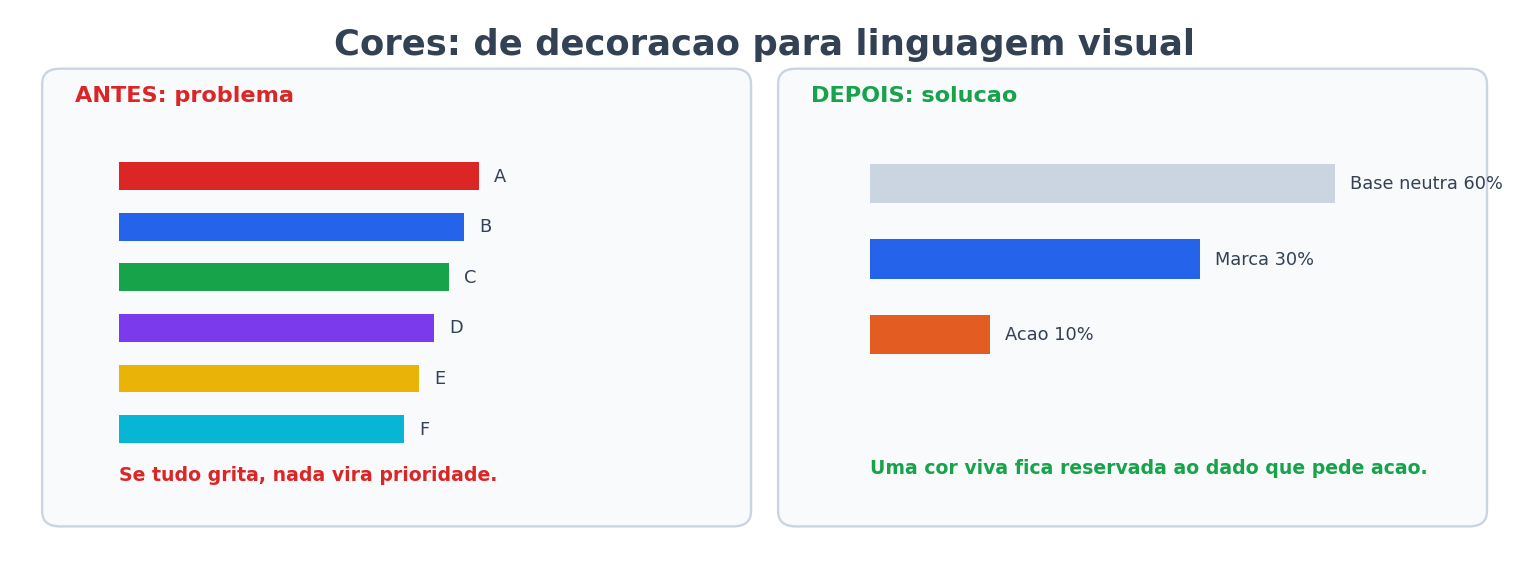
\includegraphics[width=0.58\textwidth]{semana_especial/outputs/cmp_cap1_cores.png}
\caption{Paleta de referência para dashboards. Cada cor tem uma função semântica única. Gráfico gerado pelo script \texttt{auto\_eda\_demo.py}.}
\end{figure}

\begin{BoardBox}[title=Paleta de 8 Funções --- Referência Rápida]
\begin{tabular}{@{}p{0.25cm}lll@{}}
\toprule
& \textbf{Hex} & \textbf{Função} & \textbf{Quando usar} \\
\midrule
\colorbox{colDestaque}{\phantom{M}} & \texttt{\#E35D22} & Destaque / ação urgente & O dado mais importante do dashboard \\
\colorbox{colPrimaria}{\phantom{M}} & \texttt{\#2563EB} & Primária / navegação    & Barras de base, links, filtros \\
\colorbox{colPositivo}{\phantom{M}} & \texttt{\#16A34A} & Positivo / meta atingida & Setas de alta, gaps positivos, badges OK \\
\colorbox{colAlerta}{\phantom{M}}   & \texttt{\#DC2626} & Alerta / falha / risco  & Abaixo da meta, KPI crítico \\
\colorbox{colAtencao}{\phantom{M}}  & \texttt{\#EAB308} & Atenção / monitorar     & Perto do limite, 80--99\% da meta \\
\colorbox{colNeutra}{\phantom{M}}   & \texttt{\#64748B} & Neutra / base           & Eixos, grades, texto secundário \\
\colorbox{colMarca}{\phantom{M}}    & \texttt{\#0B3D2E} & Marca / fundo escuro    & Header, rodapé, modo dark \\
\colorbox{colBgClaro}{\phantom{M}}  & \texttt{\#E2E8F0} & Background / fundo      & Área de trabalho do dashboard \\
\bottomrule
\end{tabular}
\end{BoardBox}

\paragraph{Acessibilidade e daltonismo.}
8\% dos homens e 0,5\% das mulheres têm alguma forma de daltonismo. O tipo mais comum é o deuteranopia (vermelho--verde). Regras práticas: (1) nunca use vermelho e verde como únicos diferenciadores --- adicione ícone de alta/baixa ou rótulo de texto; (2) use ferramentas como \textit{Color Oracle} ou \textit{Coblis} para simular; (3) o par azul--laranja tem alto contraste para daltonismo vermelho--verde e é a combinação padrão de grande parte dos dashboards corporativos.

\paragraph{Cor no Tableau e no QuickSight.}
No Tableau: \texttt{Format} $\to$ \texttt{Color} $\to$ \texttt{Edit Colors} define a paleta da view; use \texttt{Custom Diverging} para heatmaps; use \texttt{Single Color} com opacidade para barras onde o comprimento é o dado. No QuickSight: paletas são definidas no \textit{Theme JSON} e aplicadas globalmente no dataset; campos calculados com `ifelse` podem forçar cor semântica por condição.

% =============================================================
\section{Caminho do Olhar: Analista, Gerente e CEO}
\label{sec:olhar}
% =============================================================

Cada perfil de leitor olha para um dashboard em uma ordem diferente. Ignorar isso é o motivo pelo qual dashboards perfeitamente analíticos falham na sala de board. Entender o caminho do olhar de cada perfil é tão importante quanto escolher o gráfico certo.

\paragraph{O padrão F (analista).}
Pesquisas de eye-tracking de Jakob Nielsen (2006, \textit{Eyetracking Web Usability}) mostram que leitores técnicos percorrem o conteúdo em um padrão em forma de F: (1) leem a linha superior completa; (2) voltam ao início e leem a segunda linha; (3) varrem verticalmente o lado esquerdo em busca de palavras-chave. Implicação para dashboards: \textbf{coloque os dados mais importantes na primeira linha e no canto superior esquerdo}. O analista vai ler tudo, mas a ordem vai moldar o que ele interpreta como importante.

\paragraph{O padrão Z (executivo).}
O executivo com 5 minutos por dia varre o dashboard em Z: canto superior esquerdo $\to$ canto superior direito $\to$ diagonal $\to$ canto inferior esquerdo $\to$ canto inferior direito. Implicação: \textbf{Big Number + título-mensagem no topo esquerdo; Call to Action no rodapé direito; gráfico mais importante na diagonal}.

\begin{BoardBox}[title=Layout em Z para Dashboard Executivo]
\begin{verbatim}
[BIG NUMBER + Big Idea]  ->  [KPI2 | KPI3]
        diagonal
[Grafico diagnostico]    ->  [CALL TO ACTION]
\end{verbatim}
Percurso: (1) KPI principal com delta vs meta; (2) título-mensagem já conta a história;
(3) gráfico de diagnóstico para quem quer o detalhe; (4) CTA com verbo + prazo.
\end{BoardBox}

\begin{figure}[H]
\centering
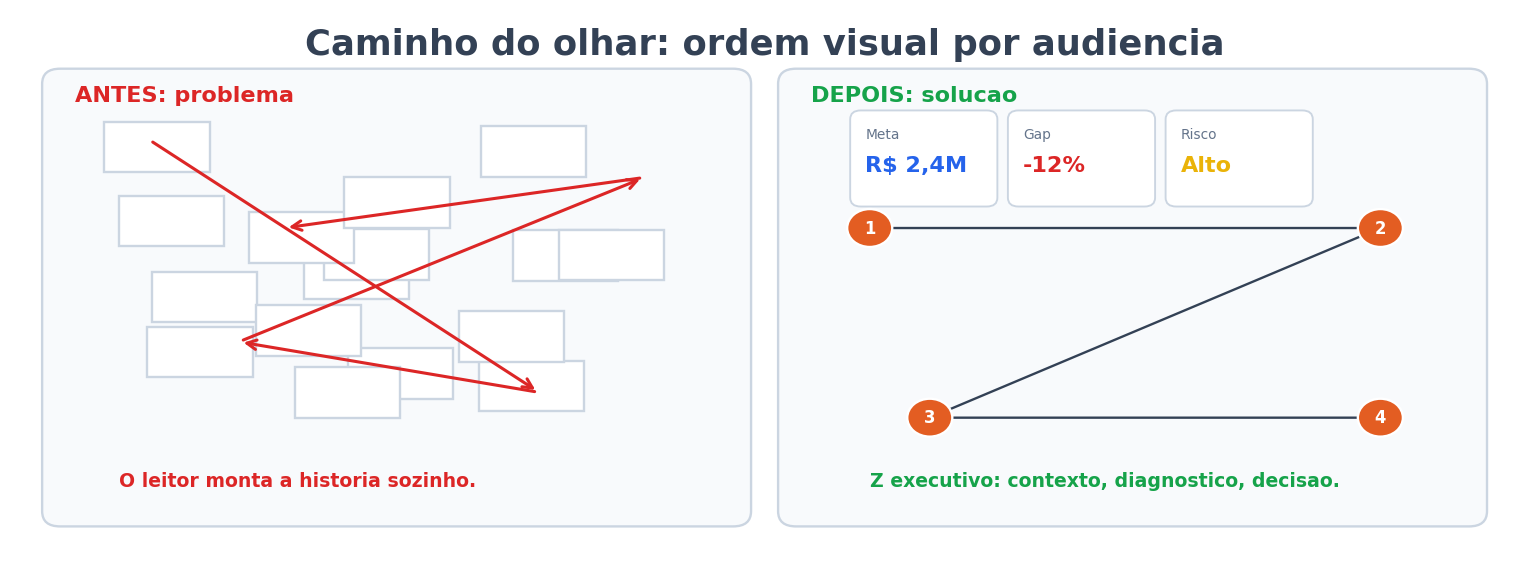
\includegraphics[width=0.58\textwidth]{semana_especial/outputs/cmp_cap1_olhar.png}
\caption{Caminho do olhar por perfil. Use esta figura em aula para mostrar que o mesmo dashboard pode falhar se a ordem visual não combinar com a audiência: o analista lê em F, o executivo varre em Z, e o gerente procura KPI, exceção e tabela de detalhe.}
\end{figure}

\paragraph{Perfil CEO: scanning semântico.}
O CEO não lê gráficos --- ele lê \emph{títulos}. Se os 4 títulos do dashboard entregam as mensagens, o CEO tomou a decisão antes de olhar qualquer eixo. A regra prática: todos os títulos de gráficos em linguagem de manchete de jornal. ``Gráfico de Barras'' $\to$ não. ``Sul lidera com 2,4$\times$ a média'' $\to$ sim.

\paragraph{Perfil gerente/gestor: diagonal + tabela.}
O gerente quer confirmar a hipótese que já tem. Ele vai direto ao gráfico que trata do seu KPI, verifica se o número confirma o que sente, e depois olha a tabela analítica no rodapé para entender as exceções. Implicação: \textbf{ofereça sempre uma tabela de detalhe no rodapé} --- ela não polui o design (ocupa a parte inferior que o executivo ignora) mas salva o gerente de tomar uma decisão com dado incompleto.

\paragraph{Perfil analista: leitura completa em espiral.}
O analista começa no Big Number, vai para o scatter, tenta reproduzir o cálculo, encontra a nota metodológica, cruza com a tabela, e só então forma uma opinião. Para esse perfil, inclua: (1) definição de todas as métricas em tooltip ou nota de rodapé; (2) período de referência explícito; (3) fonte dos dados.

% =============================================================
\section{Carga Cognitiva e Dashboard Cognitivo}
\label{sec:cognitivo}
% =============================================================

A \textbf{teoria da carga cognitiva} (Sweller, 1988) distingue três tipos de carga mental que afetam a absorção de informação. Entender isso explica por que dashboards muito elaborados technicamente falham na comunicação.

\begin{BoardBox}[title=Os 3 Tipos de Carga Cognitiva]
\begin{enumerate}
  \item \textbf{Carga intrínseca:} complexidade inerente ao conteúdo (o dado em si é complicado? a análise exige raciocínio?). Você não pode reduzir isso sem simplificar a análise.
  \item \textbf{Carga extrínseca (extraneous):} esforço causado pelo design ruim. Legenda separada que exige desvio do olhar; cores sem propósito que forçam decodificação; texto e gráfico contradizendo-se. Isso é \textbf{eliminável} com bom design.
  \item \textbf{Carga germane (útil):} esforço que forma aprendizado e schema mental. É o que sobra quando você elimina a carga extrínseca. Você quer maximizar isso.
\end{enumerate}
\smallskip
\textbf{Objetivo do bom design:} eliminar toda a carga extrínseca para liberar capacidade cognitiva para a carga útil.
\end{BoardBox}

\paragraph{Princípios de Gestalt aplicados a dashboards.}
A psicologia da Gestalt descreve como o cérebro organiza elementos visuais em padrões. Cinco princípios diretos:

\begin{BoardBox}[title=Gestalt em Dashboards]
\begin{tabular}{@{}lp{4.2cm}p{5.8cm}@{}}
\toprule
\textbf{Princípio} & \textbf{O que significa} & \textbf{Aplicação prática} \\
\midrule
Proximidade   & Elementos próximos parecem relacionados  & KPIs do mesmo tema agrupados com espaço em branco entre grupos \\
Similaridade  & Elementos parecidos parecem relacionados & Mesma cor = mesma categoria; mesmo formato = mesma hierarquia \\
Fechamento    & O cérebro completa formas incompletas    & Enclosure (caixa) ao redor de KPIs = grupo implícito sem linha pesada \\
Continuidade  & O olho segue linhas e padrões de fluxo  & Gráfico de linhas sugere tendência; use linhas de referência \\
Figura-fundo  & Um elemento se destaca, o resto recua   & 1 cor de destaque em fundo cinza é pura figura-fundo \\
\bottomrule
\end{tabular}
\end{BoardBox}

\paragraph{Dashboard cognitivo: definição.}
Um dashboard cognitivo (termo popularizado por Stephen Few em \textit{Show Me the Numbers}, 2012) é aquele que foi projetado para \emph{minimizar a carga extrínseca e maximizar a carga germane}: título-mensagem que já entrega o insight; cor de destaque que guia o olho; hierarquia visual clara (importante grande, secundário pequeno); remoção de todo chartjunk; e estrutura narrativa que replica o processo de decisão da audiência-alvo.

\begin{figure}[H]
\centering
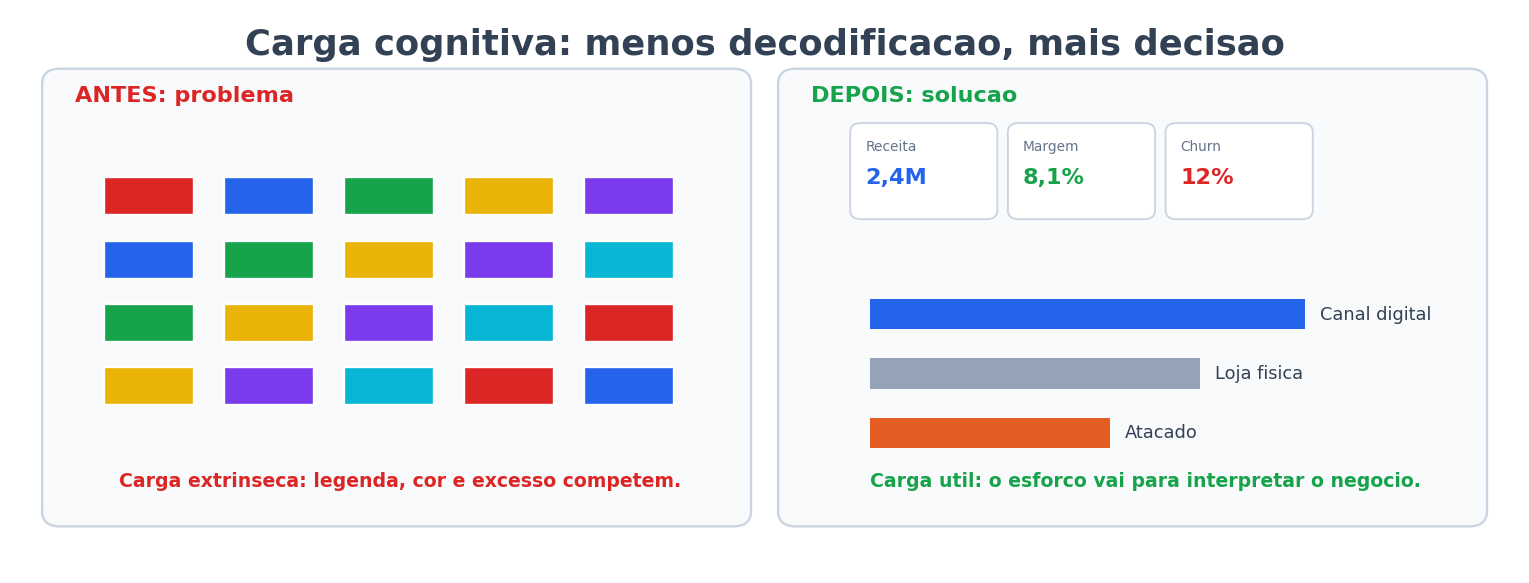
\includegraphics[width=0.58\textwidth]{semana_especial/outputs/cmp_cap1_carga.png}
\caption{Carga cognitiva aplicada a dashboards. À esquerda, o leitor gasta energia decodificando cores, formas e excesso de gráficos; à direita, a energia mental é transferida para entender o problema e decidir.}
\end{figure}

\paragraph{Número mágico 7 ± 2.}
George Miller (1956) demonstrou que a memória de trabalho humana processa 7 (mais ou menos 2) objetos simultâneos. Para dashboards: máximo de 7 KPIs na tela inicial; máximo de 7 categorias por gráfico (agrupe o restante em ``Outros''); máximo de 7 cores distintas numa paleta. Acima desses limites, a interpretação falha mesmo com dados corretos.

% =============================================================
\section{Insights Informativos}
\label{sec:insight_info}
% =============================================================

Um insight informativo é uma observação extraída dos dados que \textbf{aumenta o entendimento} de uma situação mas \emph{não orienta uma ação específica e imediata}. Ele tem valor: reduz incerteza, confirma hipóteses, fornece contexto. O problema começa quando o analista entrega \emph{apenas} insights informativos numa reunião executiva --- porque executivos não precisam de mais informação, precisam de mais clareza sobre o que fazer.

\begin{BoardBox}[title=Características de um Insight Informativo]
\begin{enumerate}
  \item \textbf{Descreve um padrão real:} algo que estava oculto nos dados e que a audiência não sabia.
  \item \textbf{É factual e verificável:} pode ser reproduzido com os mesmos dados.
  \item \textbf{Não tem urgência intrínseca:} ``interessante, mas e daí?'' é a reação esperada.
  \item \textbf{Serve de base para insights acionáveis:} todo bom insight acionável parte de um informativo.
\end{enumerate}
\end{BoardBox}

\textbf{Exemplos de insights informativos:}

\begin{itemize}
  \item ``A distribuição de Exam\_Score é aproximadamente normal (média 67,2; DP 3,9), o que indica que o dataset não tem viés de seleção severo.''
  \item ``Frequência (Attendance) tem a maior correlação com a nota final ($r = 0{,}58$), acima de horas de estudo ($r = 0{,}45$).''
  \item ``Clientes do segmento Premium têm ticket médio 3,2$\times$ maior que o segmento Standard.''
  \item ``O churn em janeiro de 2025 foi 12\% --- o maior dos últimos 24 meses.''
\end{itemize}

Insights informativos são valiosos em relatórios de EDA, em apresentações para times técnicos e em bases de conhecimento internas. O erro é confundi-los com o produto final de uma análise para a diretoria.

\begin{figure}[H]
\centering
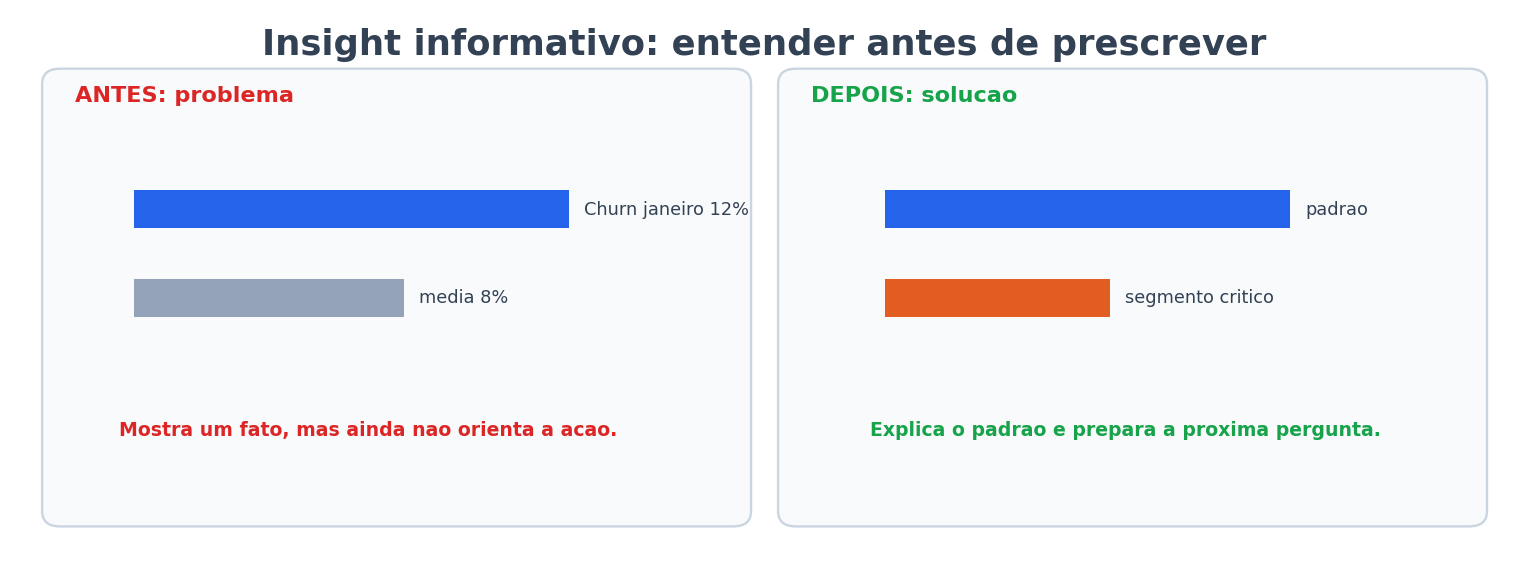
\includegraphics[width=0.58\textwidth]{semana_especial/outputs/cmp_cap1_insight_info.png}
\caption{Insight informativo em dashboard. Ele melhora o entendimento, mas ainda deixa perguntas executivas em aberto: gravidade, responsável, ação e impacto.}
\end{figure}

% =============================================================
\section{Insights Acionáveis: Do Dado à Decisão}
\label{sec:insight_acion}
% =============================================================

Este é o tópico central de qualquer analista que trabalha para a tomada de decisão. Um insight acionável \textbf{prescreve uma ação específica, direcionada a um responsável, com estimativa de impacto e prazo}. Ele não descreve o passado --- ele orienta o futuro. A diferença entre analistas júnior e sênior, na prática bancária e em qualquer grande corporação, é exatamente a capacidade de transformar observações numéricas em recomendações que mudam o comportamento de alguém.

\begin{BoardBox}[title=Fórmula do Insight Acionável --- 5 Componentes]
\begin{enumerate}
  \item \textbf{Observação:} padrão não-óbvio extraído dos dados.
  \item \textbf{Evidência:} o dado que sustenta a observação (com magnitude e significância).
  \item \textbf{Causa raiz (quando possível):} por que isso está acontecendo?
  \item \textbf{Ação prescrita:} verbo + objeto + quantidade + canal.
  \item \textbf{Impacto estimado:} resultado esperado em métrica de negócio + prazo.
\end{enumerate}
\smallskip
\textbf{Template:} ``[Observação] porque [evidência]. Se [ação prescrita] então [impacto estimado] em [prazo], responsável: [stakeholder].''
\end{BoardBox}

\paragraph{Por que a maioria dos analistas não consegue fazer isso.}
O bloqueio é conceitual: o analista foi treinado para \emph{descrever} dados, não para \emph{prescrever} ações. Descrever é seguro --- ninguém erra ao reportar que ``as vendas caíram 8\%''. Prescrever exige entender o negócio, assumir uma hipótese causal e aceitar que pode estar errado. O sênior aceita esse risco porque o valor gerado pela ação certa supera muito o custo de estar errado em uma recomendação específica.

\paragraph{Exemplos completos --- 8 domínios.}

Os exemplos a seguir seguem a estrutura de 5 componentes. Leia devagar: a diferença entre o insight informativo (coluna ``sem ação'') e o acionável (coluna ``com ação'') é a diferença de impacto na carreira de um analista.

\medskip
\textbf{Exemplo 1 --- Banco: análise de churn de cartão de crédito}

\textit{Informativo:} ``Clientes com menos de 20 transações por ano têm taxa de churn de 38\%, vs 6\% para clientes com mais de 50 transações.''

\textit{Acionável:} ``Clientes com frequência de uso $<$ 20 trans/ano e saldo médio $<$ R\$2k têm 38\% de probabilidade de cancelamento --- 3,4 pp acima da base. Acionar campanha de reengajamento personalizado via app (cashback + limite temporário) para os 8.200 clientes nesse perfil pode reverter 30\% do churn projetado, preservando R\$1,4M em receita de juros e anuidade nos próximos 12 meses. Responsável: Gerência de CRM. Prazo de implementação: 3 semanas.''

\medskip
\textbf{Exemplo 2 --- Varejo: pricing de produto}

\textit{Informativo:} ``Produtos com desconto $>$ 20\% têm margem média de $-4\%$.''

\textit{Acionável:} ``Descontos acima de 20\% em Linha Branca na Região Sul destroem R\$120k de margem por trimestre sem aumentar o volume de unidades (elasticidade próxima de zero na análise de regressão). Capear o desconto máximo em 12\% mantém a competitividade de preço percebida e projeta recuperação de R\$85k de margem trimestral. Responsável: Gerência Comercial Sul. Prazo: implementar na campanha de inverno (início de julho).''

\medskip
\textbf{Exemplo 3 --- RH: turnover de TI}

\textit{Informativo:} ``O departamento de TI tem turnover de 28\%, acima da média corporativa de 12\%.''

\textit{Acionável:} ``Engenheiros de TI com menos de 2 anos de empresa e sem promoção nos últimos 36 meses têm 3$\times$ mais probabilidade de saída que a média (28\% vs 9\%). Esse perfil representa 41 funcionários. Implantar programa de mentoria acelerada + revisão de faixa salarial para esse grupo específico pode reduzir o turnover de 28\% para 15\%, economizando R\$270k/ano em custo de reposição (R\$18k/funcionário $\times$ 15 saídas evitadas). Responsável: HRBP de TI + Diretor de Engenharia. Prazo: começar em 30 dias para impactar a janela de avaliação semestral.''

\medskip
\textbf{Exemplo 4 --- Saúde: readmissão hospitalar}

\textit{Informativo:} ``Pacientes com diabetes + hipertensão têm taxa de readmissão em 30 dias de 34\%.''

\textit{Acionável:} ``Pacientes diabéticos com HbA1c $>$ 9 e diagnóstico de HAS que receberam alta sem consulta de retorno agendada têm 34\% de readmissão em 30 dias vs 8\% quando o retorno está agendado. Implementar protocolo de agendamento obrigatório na alta para os 1.200 pacientes nesse perfil anual pode evitar 312 readmissões, economizando R\$3,7M (R\$12k/internação), além de melhorar o indicador de qualidade AHRQ-PSI. Responsável: Gerência de Assistência. Prazo: protocolo ativo no próximo semestre.''

\medskip
\textbf{Exemplo 5 --- E-commerce: logística}

\textit{Informativo:} ``O estado do Amazonas tem atraso médio de 4,7 dias acima da estimativa.''

\textit{Acionável:} ``Pedidos de Eletrônicos em AM com prazo estimado $<$ 7 dias chegam em média 4,7 dias atrasados, gerando review médio de 2,8 estrelas e taxa de devolução 18\% acima da média. Substituir a transportadora atual por operador regional com SLA de 5 dias para essa rota reduz o atraso estimado em 70\%, projeta melhora do review para 4,1 estrelas e reduz devoluções em R\$95k/semestre. Responsável: Gerência de Logística. Prazo: RFP para transportadora em 45 dias.''

\medskip
\textbf{Exemplo 6 --- Fintech: crédito}

\textit{Informativo:} ``A inadimplência de empréstimo pessoal cresceu 3 pp em Q1/2026.''

\textit{Acionável:} ``Clientes de empréstimo pessoal com renda variável (profissional autônomo) que acessaram o produto em fevereiro/março têm inadimplência de 19\%, contra 7\% para clientes com renda fixa. O crescimento de 3 pp na inadimplência total é explicado em 78\% por esse segmento (análise de decomposição). Ajustar a política de crédito para limitar o LTV de empréstimo pessoal a 60\% da renda variável comprovada pode reduzir a inadimplência desse perfil de 19\% para 10\%, preservando R\$4,2M em provisão de crédito no próximo trimestre. Responsável: Gerência de Risco de Crédito. Prazo: vigência imediata para novas contratações.''

\medskip
\textbf{Exemplo 7 --- Educação (dataset StudentPerformance)}

\textit{Informativo:} ``Frequência (Attendance) tem correlação de 0,58 com Exam\_Score, sendo o preditor mais forte entre as variáveis numéricas.''

\textit{Acionável:} ``Alunos com frequência $<$ 75\% nos meses de março--abril têm nota final média 9,3 pts abaixo da média geral (67,2), e 34\% deles reprovam. Implementar sistema de alerta automático por WhatsApp para responsáveis quando o aluno atingir 3 faltas consecutivas pode recuperar 40\% desses alunos (baseado em piloto de 2024), reduzindo a taxa de reprovação de 8\% para 4,8\%, equivalendo a 216 alunos aprovados adicionais por semestre. Responsável: Coordenação Pedagógica + TI. Prazo: sistema ativo no início do semestre seguinte.''

\medskip
\textbf{Exemplo 8 --- Marketing digital: aquisição}

\textit{Informativo:} ``O CAC médio pelo canal Google Ads é R\$48, contra R\$31 pelo canal Organic.''

\textit{Acionável:} ``O canal Google Ads tem CAC 55\% maior que o orgânico, mas o LTV dos clientes adquiridos por Google Ads é apenas 8\% maior (R\$320 vs R\$296). O ROI ajustado ao LTV do canal pago é negativo ($-$4\%) no primeiro ano. Redirecionar 40\% do orçamento de Google Ads para SEO/Content durante 6 meses projeta redução do CAC médio de R\$48 para R\$35, com impacto de $-$12\% no volume de aquisição no curto prazo mas retorno positivo a partir do mês 8. Responsável: Gerência de Marketing. Prazo: próximo ciclo de orçamento (Q3 2026).''

\paragraph{Como treinar a habilidade de gerar insights acionáveis.}
O caminho mais rápido é forçar a pergunta ``\emph{e daí?}'' sobre cada dado encontrado. Toda vez que você escrever uma observação, pergunte: ``E daí?'' até chegar num verbo de ação ligado a um responsável. Veja a cadeia:

\begin{BoardBox}[title=A Cadeia ``E Daí?'' --- Exercício Prático]
\textbf{Observação inicial:} ``O churn subiu 3\%.'' \quad \textbf{E daí?}\\
\textbf{Nível 2:} ``Clientes do segmento X estão cancelando mais.'' \quad \textbf{E daí?}\\
\textbf{Nível 3:} ``Clientes do segmento X com produto Y cancelam 4$\times$ mais no 3$^\circ$ mês.'' \quad \textbf{E daí?}\\
\textbf{Nível 4:} ``O problema é que o onboarding do produto Y não é completado por 60\% dos clientes.'' \quad \textbf{E daí?}\\
\textbf{Insight acionável:} ``Criar fluxo de onboarding guiado no app para produto Y, com nudge no dia 15, pode reduzir o churn do segmento X de 18\% para 8\%, preservando R\$XX em ARR. Responsável: PM + CRM. Prazo: 4 semanas.''
\end{BoardBox}

\begin{figure}[H]
\centering
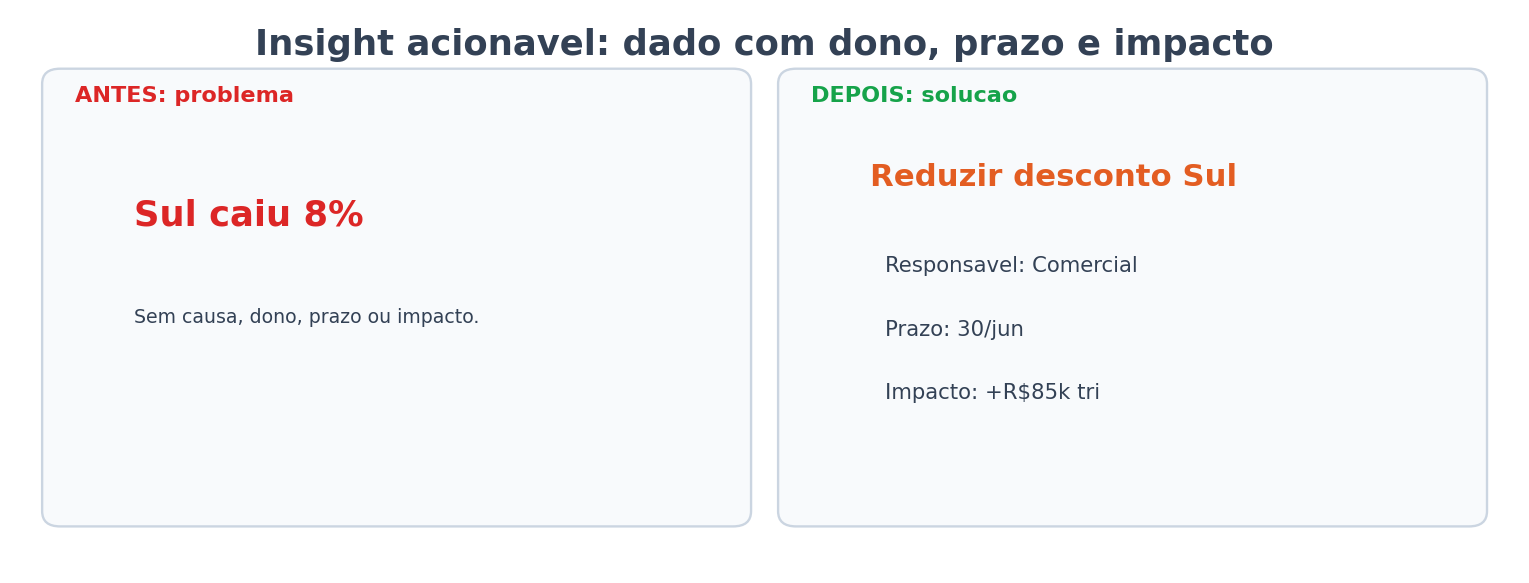
\includegraphics[width=0.58\textwidth]{semana_especial/outputs/cmp_cap1_insight_acionavel.png}
\caption{Dashboard sem ação versus dashboard com insight acionável. O segundo não apenas descreve o problema: ele explicita o que fazer, quem deve fazer, até quando e qual impacto esperado.}
\end{figure}

% =============================================================
\section{Dashboard as Code: AWS e QuickSight}
\label{sec:daac}
% =============================================================

\textbf{Dashboard as Code (DaC)} é a prática de definir, versionar e publicar dashboards inteiramente via código e infraestrutura como código (IaC), eliminando configuração manual via interface gráfica. Os benefícios diretos para um time de analytics bancário são: rastreabilidade via Git, reprodutibilidade entre ambientes (dev/homol/prod), revisão de mudanças por Pull Request, e orquestração programática de dezenas de dashboards.

\paragraph{AWS QuickSight e as APIs de criação.}
O QuickSight expõe uma API REST completa (\textit{aws quicksight} via Boto3 ou CLI) que permite criar e atualizar todos os recursos: datasets, análises, dashboards e permissões. Os objetos principais na hierarquia são:

\begin{BoardBox}[title=Hierarquia de Objetos no QuickSight]
\begin{tabular}{@{}llp{6.5cm}@{}}
\toprule
\textbf{Objeto} & \textbf{API} & \textbf{Descrição} \\
\midrule
DataSource    & \texttt{create-data-source}    & Conexão ao S3/Redshift/Athena/RDS \\
DataSet       & \texttt{create-data-set}       & Schema, joins, campos calculados, filtros de linha \\
Analysis      & \texttt{create-analysis}       & Canvas de edição (não publicado) \\
Dashboard     & \texttt{create-dashboard}      & Versão publicada de uma Analysis \\
Template      & \texttt{create-template}       & Snapshot de uma Analysis reutilizável cross-account \\
Theme         & \texttt{create-theme}          & Paleta de cores, fontes e layout globais \\
\bottomrule
\end{tabular}
\end{BoardBox}

\paragraph{Fluxo conceitual do Dashboard as Code.}
Para esta aula, o importante não é decorar código de Boto3 ou CDK. O ponto central é entender que o dashboard deixa de ser uma peça manual feita no clique e passa a ser um artefato governado: nasce de uma regra de negócio, é versionado, revisado, homologado e publicado com rastreabilidade.

\begin{figure}[H]
\centering
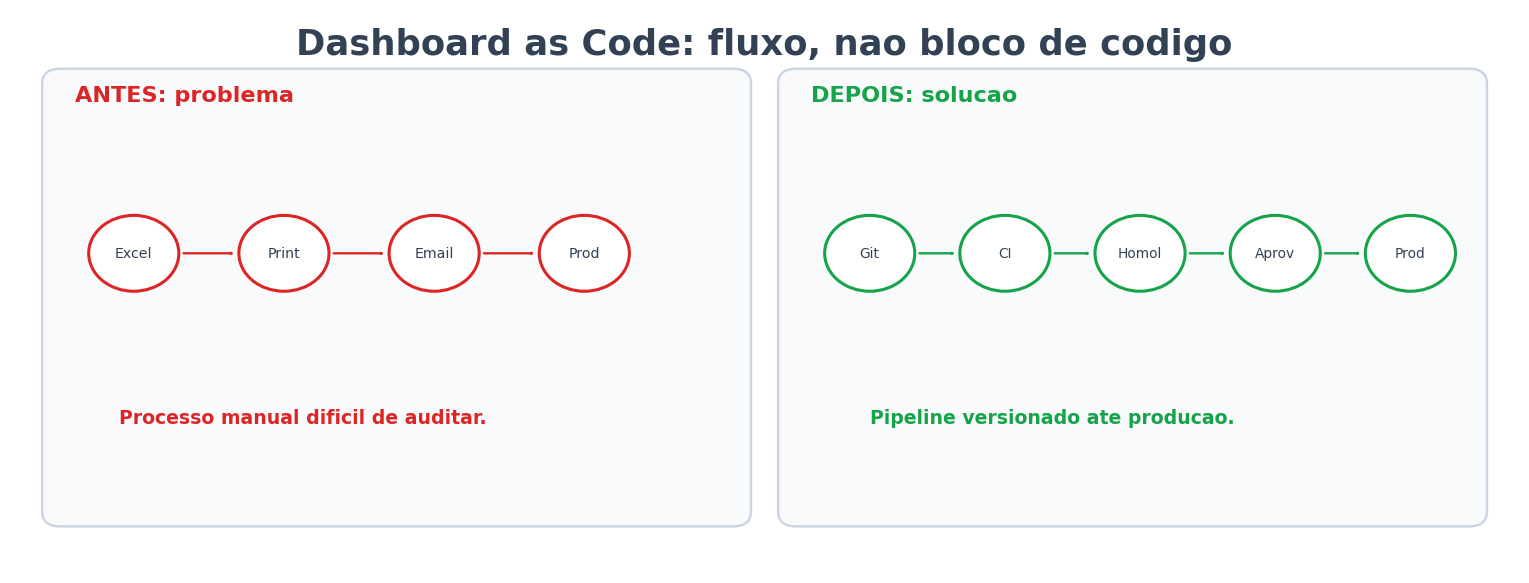
\includegraphics[width=0.58\textwidth]{semana_especial/outputs/cmp_cap1_dac.png}
\caption{Fluxo conceitual de Dashboard as Code. A criação programática só faz sentido quando protege governança: regra de negócio clara, definição versionada, revisão por pares, homologação e publicação controlada.}
\end{figure}

\paragraph{Fluxo de trabalho DaC com Git.}
O padrão recomendado para times de analytics em bancos: (1) \texttt{feature/dashboard-churn} branch; (2) código Python com definição de datasets + análise em JSON (exportado via \texttt{describe-analysis-definition}); (3) PR com revisão de outro analista; (4) merge em \texttt{main} dispara GitHub Actions que chama \texttt{boto3.update\_dashboard}; (5) tags de versão correspondem a versões do QuickSight.

\paragraph{Asset Bundle Export/Import.}
Para migração entre contas (dev $\to$ prod) sem recriar tudo manualmente, o QuickSight oferece desde 2023 o \textbf{Asset Bundle} API: exporta análises, dashboards, datasets e temas em JSON e importa em outra conta com substituição de ARNs. Isso é o equivalente ao \texttt{terraform plan/apply} para dashboards.

% =============================================================
\section{AED Automática: Bibliotecas, Relatórios e Interpretação}
\label{sec:autoeda}
% =============================================================

As bibliotecas de AED automática (profiling) fazem em uma linha o que levaria horas de código manual: calculam estatísticas descritivas, detectam outliers, mapeiam correlações, identificam dados ausentes, avaliam distribuições e geram relatório HTML completo. Elas não substituem a análise --- substituem a parte mecânica para que o analista foque na interpretação.

\begin{BoardBox}[title=Principais Bibliotecas de AED Automática (Python)]
\begin{tabular}{@{}lp{3.5cm}p{5.8cm}@{}}
\toprule
\textbf{Biblioteca} & \textbf{Melhor para} & \textbf{Diferencial} \\
\midrule
\texttt{ydata-profiling} & Relatório completo solo & 1 linha; HTML interativo; detecta correlações, outliers, duplicatas, alertas de qualidade \\
\texttt{sweetviz}        & Comparação de grupos    & Visualiza diferenças entre treino/teste ou segmentos lado a lado; target analysis \\
\texttt{autoviz}         & Visualizações rápidas   & Gera gráficos automaticamente sem HTML; bom para exploração rápida \\
\texttt{D-Tale}          & Exploração interativa   & Interface web local tipo Excel interativo; edição de dados em tempo real \\
\texttt{lux}             & Recomendação automática & Sugere visuais relevantes contextualizados ao DataFrame; integra Jupyter \\
\bottomrule
\end{tabular}
\end{BoardBox}

\paragraph{Como ler um relatório automático.}
Nesta aula, não precisamos decorar comandos. O que importa é saber interpretar o HTML produzido por essas ferramentas. Primeiro olhe os \textbf{alertas de qualidade}: dados ausentes, duplicatas, cardinalidade alta e colunas constantes. Depois leia as \textbf{distribuições}: assimetria, outliers e concentração. Em seguida, veja \textbf{correlações e associações}: elas sugerem hipóteses, mas não provam causalidade. Por fim, transforme o relatório em perguntas de negócio: ``qual variável explica o resultado?'', ``qual grupo merece intervenção?'', ``que dado precisa ser validado antes da decisão?''.

\begin{figure}[H]
\centering
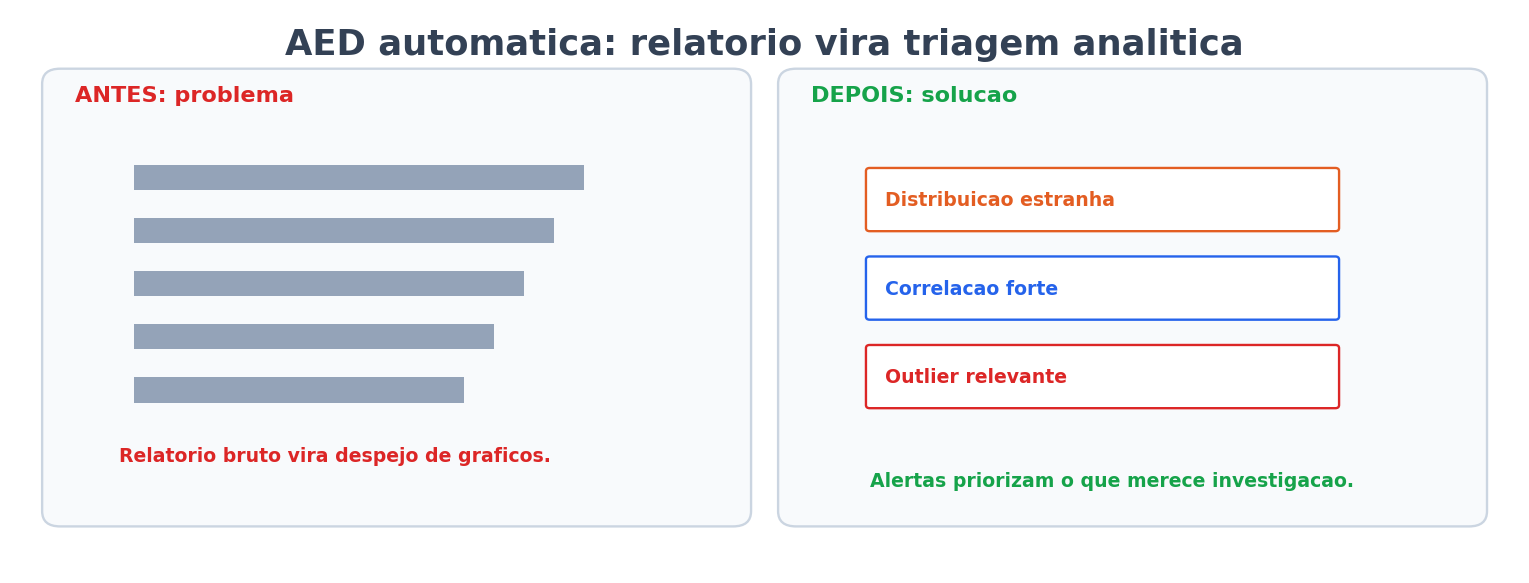
\includegraphics[width=0.58\textwidth]{semana_especial/outputs/cmp_cap1_autoeda.png}
\caption{Fluxo de leitura da AED automática. O HTML é um ponto de partida: ele encontra sinais, mas o analista precisa explicar o significado e formular a próxima pergunta.}
\end{figure}

\paragraph{Exemplo real: StudentPerformanceFactors.csv.}

Rodamos \texttt{ydata-profiling} (modo minimal, 6607 registros, 20 variáveis) e \texttt{sweetviz} no dataset deste curso. Os relatórios HTML estão em \texttt{semana\_especial/outputs/}:
\begin{itemize}
  \item \texttt{ydata\_profiling\_report.html} --- perfil completo com alertas de qualidade, correlações, distribuições
  \item \texttt{sweetviz\_report.html} --- target analysis com Exam\_Score como variável alvo
\end{itemize}

Em aula, use esses relatórios como material de inspeção: eles mostram distribuições, correlações, scatterplots e variáveis categóricas. O PDF mantém apenas o comparativo acima para não repetir quatro figuras exploratórias onde uma síntese visual resolve melhor.

\paragraph{Alertas automáticos que o ydata-profiling detecta.}
O relatório HTML sinaliza automaticamente: variáveis com $>$ 5\% de dados ausentes; colunas com alta correlação ($>$ 0,9) que indicam redundância; variáveis com cardinalidade muito alta (suspeita de ID); distribuições muito assimétricas (candidatas a transformação log); valores constantes ou quase-constantes.

\paragraph{Quando NÃO usar AED automática.}
Quando o dataset tem $>$ 10M de linhas (o relatório trava ou demora demais --- use uma amostra estratificada de 50k--100k linhas); quando as variáveis têm semântica muito específica do negócio que a biblioteca não conhece (ex.: códigos de agência bancária precisam de dicionário manual); quando o objetivo já é confirmatory (você já sabe o que procura --- vá direto).

% =============================================================
\section{Arquitetura de Agentes para AED e Dashboards}
\label{sec:agentes}
% =============================================================

A abordagem de agentes para análise de dados está passando de experimento acadêmico para realidade em grandes bancos e fintechs em 2025--2026. A ideia central é substituir o fluxo manual linear (analista faz EDA $\to$ analista faz perguntas $\to$ analista constrói dashboard) por um \textbf{pipeline orquestrado de agentes especializados}, cada um responsável por uma etapa e passando seu output como contexto estruturado para o próximo.

\paragraph{A arquitetura descrita.}
O pipeline que estamos construindo no banco tem a seguinte cadeia:

\begin{BoardBox}[title=Pipeline Multi-Agente --- Etapas]
\begin{enumerate}
  \item \textbf{Agente Discovery:} lê o contrato de negócio (dores, KPIs, audiência), carrega o dataset, calcula estatísticas descritivas, mapeia correlações, detecta outliers. Output: JSON com contexto estruturado.
  \item \textbf{Agente de Insights:} recebe o JSON do Agente 1, consulta a base especializada de insights (seção 9), e gera insights acionáveis candidatos com score de relevância.
  \item \textbf{Agente de Storyboard:} define Big Idea, estrutura 3 zonas (Contexto/Diagnóstico/Recomendação), monta a sequência de gráficos e os títulos-mensagem.
  \item \textbf{Agente Protótipo:} gera HTML completo do dashboard com Chart.js, auto-contido, com dados reais do dataset. Output: \texttt{prototipo.html}.
  \item \textbf{Agente de Infraestrutura (AWS):} recebe o protótipo aprovado, converte para definição QuickSight (JSON/API), cria DataSet + Analysis + Dashboard via Boto3.
  \item \textbf{Agente de Documentação:} gera changelog, dicionário de métricas e runbook automaticamente a partir dos metadados dos agentes anteriores.
\end{enumerate}
\smallskip
\textbf{Orquestrador:} LangChain / LangGraph / AWS Step Functions (para pipelines produtivos em nuvem).
\end{BoardBox}

\begin{figure}[H]
\centering
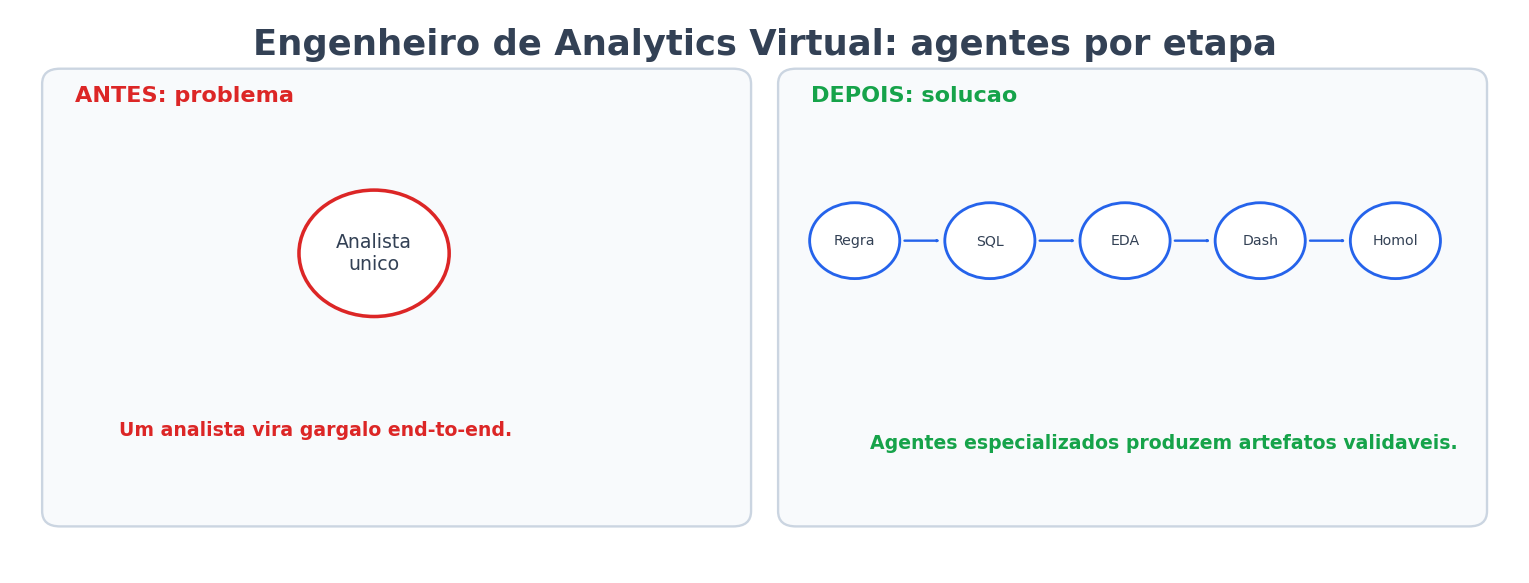
\includegraphics[width=0.58\textwidth]{semana_especial/outputs/cmp_cap1_agentes.png}
\caption{Arquitetura lúdica do Engenheiro de Analytics Virtual. A ideia prática é end-to-end: da regra de negócio até a publicação do dashboard, cada agente produz um artefato que pode ser revisado e homologado.}
\end{figure}

\paragraph{Protótipo gerado pelo pipeline.}

O script \texttt{agente\_prototipo\_html.py} executa os Agentes 1--4 localmente, sem LLM externo, usando apenas pandas e Chart.js. O arquivo \texttt{prototipo\_dashboard\_agente.html} está em \texttt{semana\_especial/outputs/}. Ele demonstra a estrutura que o pipeline mais completo (com LLM) produziria.

\paragraph{Como funcionaria na prática.}
Imagine que a área de negócio pede: ``o churn do cartão Premium subiu e precisamos decidir uma campanha''. O Agente de Negócio transforma isso em contrato: audiência, dor, métrica-alvo, restrições e prazo. O Agente de Dados valida tabelas, chaves, granularidade e qualidade. O Agente SQL cria ou sugere views analíticas. O Agente EDA procura padrões. O Agente de Insights transforma padrões em recomendações. O Agente Storyboard escolhe a sequência narrativa. O Agente Protótipo gera um HTML para homologação rápida. Só depois de aprovado entram os agentes de produção: criação de dataset, dashboard no BI, permissões, documentação e changelog.

\begin{BoardBox}[title=Artefatos por Agente]
\begin{tabular}{@{}lp{8.7cm}@{}}
\toprule
\textbf{Agente} & \textbf{Artefato entregue} \\
\midrule
Negócio & contrato de análise: dor, KPI, audiência, decisão esperada \\
Dados/SQL & tabela, view ou consulta validada com dicionário de métricas \\
EDA & resumo visual de padrões, outliers, correlações e alertas \\
Insights & 2--3 recomendações acionáveis com impacto e responsável \\
Storyboard & Big Idea, zonas do dashboard e títulos-mensagem \\
Protótipo & HTML navegável para homologação com usuário \\
Produção & dashboard publicado, permissões, documentação e versão \\
\bottomrule
\end{tabular}
\end{BoardBox}

\paragraph{Padrões de multi-agente: ReAct, Chain-of-Thought e Tool-Use.}
Três padrões são relevantes para o pipeline de analytics: (1) \textbf{ReAct} (Yao et al., 2022) --- o agente raciocina (\textit{Thought}) e então age (\textit{Action}), iterando até atingir o objetivo; ideal para o Agente de Insights que precisa testar hipóteses. (2) \textbf{Chain-of-Thought} (Wei et al., 2022) --- o agente externaliza o raciocínio passo a passo antes de entregar o output; útil no Agente de Storyboard para justificar cada decisão de layout. (3) \textbf{Tool-Use / Function-Calling} (OpenAI, 2023) --- o agente chama funções externas (Boto3, Tableau API, base de dados) de forma estruturada; é o que habilita o Agente de Infraestrutura a criar dashboards reais no QuickSight.

% =============================================================
\section{Como Criar Insights Acionáveis: Base Especializada}
\label{sec:insight_base}
% =============================================================

O maior gargalo para gerar insights acionáveis em escala (em um time de 20 analistas, para dezenas de produtos) é a \textbf{inconsistência de qualidade}. Cada analista usa sua própria definição do que é um insight, seu próprio template, sua própria escala de urgência. O resultado: 80\% dos ``insights'' entregues são observações descritivas, e os executivos param de ler relatórios de dados.

A solução é criar uma \textbf{base especializada em insights}: um repositório estruturado (tabela, vector store ou knowledge base) que contém exemplos de alta qualidade validados pelo negócio, que serve de referência para analistas humanos e de few-shot context para agentes de IA.

\begin{figure}[H]
\centering
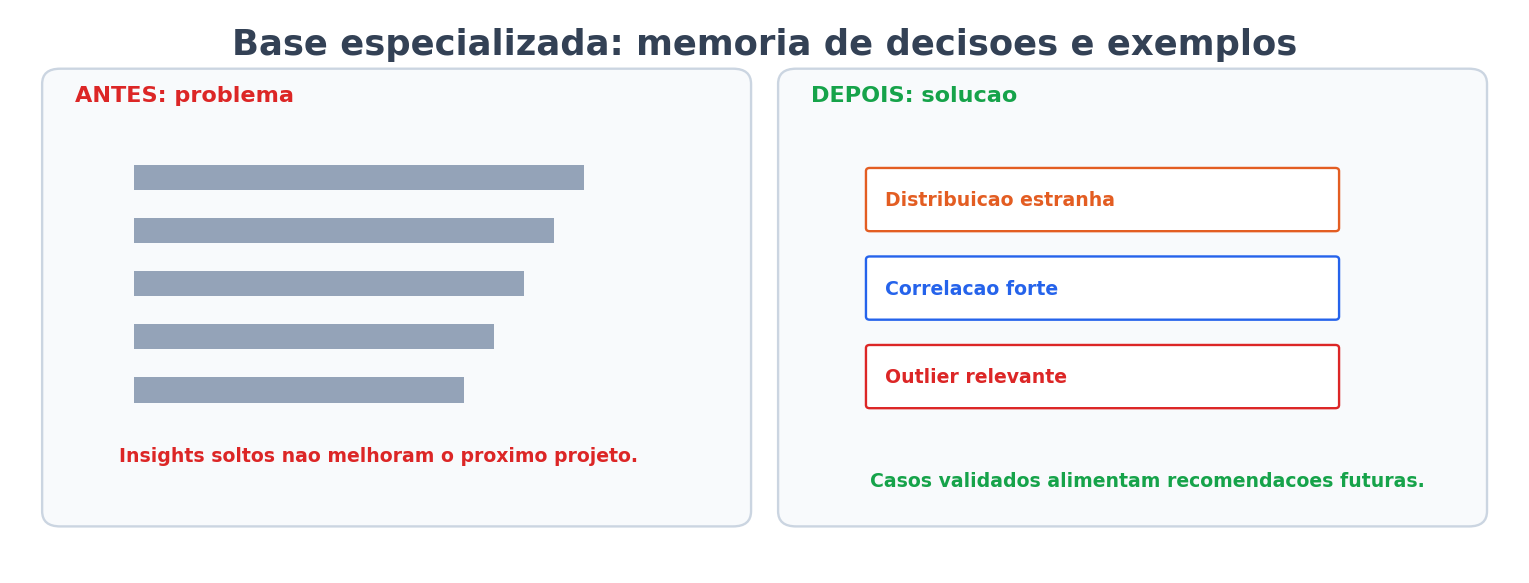
\includegraphics[width=0.58\textwidth]{semana_especial/outputs/cmp_cap1_base_insights.png}
\caption{Base especializada de insights. Ela funciona como memória de qualidade: exemplos validados alimentam novos agentes e padronizam o que a turma deve chamar de insight acionável.}
\end{figure}

\begin{BoardBox}[title=Tabela \texttt{insight\_base}]
\small
\begin{tabular}{@{}p{3.2cm}p{2.2cm}p{5.6cm}@{}}
\toprule
\textbf{Campo} & \textbf{Tipo} & \textbf{Descrição} \\
\midrule
\texttt{insight\_id}    & VARCHAR(20)  & Identificador único (ex.: INS-001) \\
\texttt{dominio}        & VARCHAR(50)  & Área do negócio (Crédito, Varejo, RH\ldots) \\
\texttt{tipo}           & ENUM         & \texttt{acionavel} | \texttt{informativo} \\
\texttt{titulo}         & VARCHAR(200) & Frase-resumo do insight (padrão + ação) \\
\texttt{observacao}     & TEXT         & Padrão detectado com dado concreto \\
\texttt{evidencia}      & TEXT         & Estatística que sustenta (n, correlação, delta) \\
\texttt{causa\_raiz}    & TEXT         & Hipótese causal (quando disponível) \\
\texttt{acao}           & TEXT         & Verbo + objeto + canal + quantidade \\
\texttt{impacto}        & TEXT         & Resultado esperado em métrica de negócio \\
\texttt{stakeholder}    & VARCHAR(100) & Responsável pela ação \\
\texttt{urgencia}       & ENUM         & \texttt{Alta} | \texttt{Media} | \texttt{Baixa} \\
\texttt{prazo\_sugerido}& VARCHAR(50)  & Ex.: ``Q3 2026'', ``próximo semestre'' \\
\texttt{fonte}          & VARCHAR(200) & Dataset / tabela de origem \\
\texttt{validado\_por}  & VARCHAR(100) & Analista ou gestor que validou o insight \\
\texttt{data\_criacao}  & DATE         & Data de geração \\
\texttt{embedding}      & VECTOR(1536) & Embedding semântico para busca por similaridade \\
\bottomrule
\end{tabular}
\end{BoardBox}

\paragraph{Exemplo real gerado pelo pipeline.}

O arquivo \texttt{insight\_base\_exemplo.csv} em \texttt{semana\_especial/outputs/} contém 3 registros gerados automaticamente pelo Agente de Insights sobre o dataset StudentPerformance. A estrutura é a mesma para qualquer domínio.

\paragraph{Como o agente usa a base para gerar novos insights.}
O Agente de Insights (seção anterior) faz o seguinte: (1) calcula as estatísticas do dataset atual (Agente 1); (2) busca na base especializada os 3--5 insights mais similares por domínio + tipo de padrão (busca vetorial por embedding semântico); (3) usa esses exemplos como \textit{few-shot context} no prompt do LLM; (4) o LLM gera um insight acionável seguindo exatamente o schema. A qualidade dos exemplos na base determina diretamente a qualidade dos insights gerados.

\begin{BoardBox}[title=Uso da Base pelo Agente]
Na prática, o agente não ``inventa'' do zero. Ele recebe o contexto do dataset, busca exemplos parecidos na base, compara o padrão atual com casos já validados, e então gera uma recomendação no mesmo formato: observação, evidência, ação, impacto, responsável e prazo. Isso reduz variação de qualidade entre analistas e evita que uma observação descritiva seja vendida como insight.
\end{BoardBox}

\paragraph{Construir a base de forma contínua.}
A base deve crescer com cada projeto: (1) analista gera insights; (2) gestor valida e adiciona o campo \texttt{validado\_por}; (3) após 6 meses, mede-se a taxa de adoção das ações recomendadas e o impacto realizado vs estimado --- isso cria um loop de melhoria contínua na qualidade dos insights gerados.

Em produção na AWS, a base pode ser: uma tabela no DynamoDB (para escrita/leitura rápida por analistas) + uma coleção no Amazon Bedrock Knowledge Base (para busca semântica pelo agente) + um bucket S3 como backup e auditoria.

% =============================================================
\section*{Referências: Cognição, Insights e Automação}
% =============================================================

As referências abaixo estão disponíveis para download e leitura. As marcadas com \textbf{[BANCO]} são particularmente relevantes para aplicação em analytics bancário.

\begin{itemize}
  \item \textbf{Few, S. (2006).} \textit{Information Dashboard Design}. O'Reilly. --- Framework de carga cognitiva aplicado a dashboards; dashboards cognitivos. \textbf{[BANCO]}

  \item \textbf{Few, S. (2012).} \textit{Show Me the Numbers} (2ª ed.). Analytics Press. --- Teoria de design de gráficos; data-ink ratio; pré-atenção.

  \item \textbf{Sweller, J. (1988).} ``Cognitive Load During Problem Solving: Effects on Learning''. \textit{Cognitive Science}, 12(2), 257--285. --- Teoria original da carga cognitiva. DOI: 10.1207/s15516709cog1202\_4

  \item \textbf{Miller, G. A. (1956).} ``The Magical Number Seven, Plus or Minus Two''. \textit{Psychological Review}, 63(2), 81--97. --- Limite de memória de trabalho; regra dos 7 KPIs. DOI: 10.1037/h0043158

  \item \textbf{Ware, C. (2004).} \textit{Information Visualization: Perception for Design} (2ª ed.). Morgan Kaufmann. --- Fundamentos neurocientíficos de visualização. \textbf{[BANCO]}

  \item \textbf{Nielsen, J. \& Pernice, K. (2010).} \textit{Eyetracking Web Usability}. New Riders. --- Padrões F e Z de leitura; eye-tracking em interfaces.

  \item \textbf{Duarte, N. (2019).} \textit{DataStory: Explain Data and Inspire Action Through Story}. Ideapress. --- Big Idea; estrutura narrativa SCR; pitch de dados.

  \item \textbf{Tufte, E. R. (1983).} \textit{The Visual Display of Quantitative Information}. Graphics Press. --- Data-ink ratio; chartjunk; small multiples.

  \item \textbf{Yao, S. et al. (2022).} ``ReAct: Synergizing Reasoning and Acting in Language Models''. \textit{arXiv:2210.03629}. --- Padrão ReAct para agentes LLM. \url{https://arxiv.org/abs/2210.03629} \textbf{[BANCO]}

  \item \textbf{Wei, J. et al. (2022).} ``Chain-of-Thought Prompting Elicits Reasoning in Large Language Models''. \textit{arXiv:2201.11903}. --- Chain-of-Thought para agentes de análise. \url{https://arxiv.org/abs/2201.11903} \textbf{[BANCO]}

  \item \textbf{Wang, L. et al. (2023).} ``A Survey on Large Language Model based Autonomous Agents''. \textit{arXiv:2308.11432}. --- Survey completo de arquiteturas de agentes LLM. \url{https://arxiv.org/abs/2308.11432} \textbf{[BANCO]}

  \item \textbf{Hong, S. et al. (2024).} ``Data Interpreter: An LLM Agent for Data Science''. \textit{arXiv:2402.18679}. --- Agente específico para AED automática com LLMs. \url{https://arxiv.org/abs/2402.18679} \textbf{[BANCO]}

  \item \textbf{AWS. (2024).} \textit{Amazon QuickSight Developer Guide}. --- APIs de criação programática de dashboards. \url{https://docs.aws.amazon.com/quicksight/latest/developerguide/}

  \item \textbf{Pedregosa, F. et al. (2011).} ``Scikit-learn: Machine Learning in Python''. \textit{JMLR}, 12, 2825--2830. --- Referência para bibliotecas de EDA automatizada. DOI: 10.5555/1953048.2078195
\end{itemize}

\clearpage
% =============================================================================
% Semana Especial --- Revisão Unidade II + Apresentação em Grupo
% Aula 1: 04/05/2026 --- Revisão completa da Unidade II
% Aula 2: 18/05/2026 --- Apresentações em grupo (última aula antes das provas)
%
% COMPILAÇÃO: incluir em aula/main.tex com \input{semana_especial/semana_especial}
% \includegraphics paths são relativos ao diretório de main.tex (aula/)
% =============================================================================

\chapter{Semana Especial (04/05 + 18/05/2026)\\[4pt]Revisão Unidade~II e Dashboard em Grupo}

Este impresso cobre as duas últimas aulas antes das provas. No dia \textbf{04/05} fazemos a revisão de toda a Unidade~II. No dia \textbf{18/05} cada grupo apresenta o dashboard no Tableau --- como está descrito na Parte~III deste documento, que você já recebe hoje para ter duas semanas de preparo. As provas começam na semana de \textbf{25/05}.

% ============================================================
\section*{\Large PARTE I --- REVISÃO DA UNIDADE II (04/05/2026)}
% ============================================================

% -------------------------------------------------------
\section{AED vs.\ Análise Explanatória}
% -------------------------------------------------------

Na Unidade~I vocês exploraram dados para \emph{entender}: histogramas, boxplots, correlações, dados ausentes. A pergunta que guiava cada análise era ``o que os dados me dizem?'' A Unidade~II começa com uma mudança radical de perspectiva. A pergunta agora é outra: \textit{``como eu conto essa história para que alguém tome uma decisão?''}

Quando você sai do papel de analista e entra no papel de comunicador, você faz análise \textbf{explanatória}. A audiência mudou: não é mais você mesmo --- é o CEO, o gerente, o comitê de crédito. Essas pessoas não têm tempo para ver os 200 gráficos que você gerou. Elas precisam de uma mensagem clara suportada pelas evidências certas.

O erro mais comum de analistas iniciantes é mostrar todo o processo exploratório para uma audiência executiva. O resultado: confusão, perda de tempo, e a descoberta mais importante se perde no meio de 30 gráficos. Na análise explanatória, você já sabe a história que vai contar e escolhe \emph{apenas} os gráficos que a sustentam.

\begin{BoardBox}[title=AED vs.\ Explanatória]
\begin{tabular}{@{}lp{4.2cm}p{5.2cm}@{}}
\toprule
 & \textbf{Exploratória (AED)} & \textbf{Explanatória} \\
\midrule
Audiência & O analista & CEO, gerente, investidor \\
Objetivo  & Entender o dado & Provocar uma decisão \\
Linguagem & ``O dado mostra X'' & ``O que este dado muda no que você faz?'' \\
Visuais   & Centenas (maioria descartada) & Só os que servem à mensagem \\
\bottomrule
\end{tabular}
\end{BoardBox}

Toda vez que você estiver construindo uma apresentação, faça esta pergunta para cada gráfico: ``este visual serve à mensagem ou serve à minha curiosidade?'' Se for a segunda opção, ele vai para o apêndice.

\begin{center}
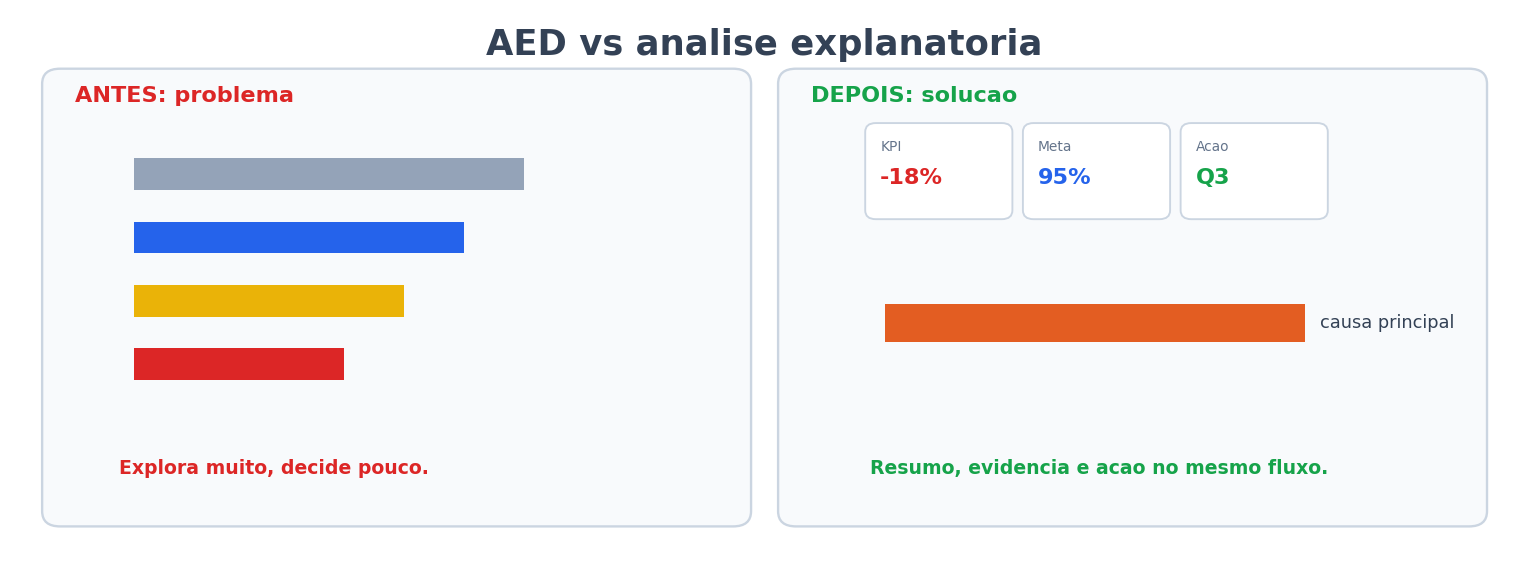
\includegraphics[width=0.58\textwidth]{semana_especial/outputs/cmp_cap2_aed_explanatoria.png}
\end{center}

\textbf{Exemplo prático:} você está analisando dados de alunos em uma instituição de ensino. Na perspectiva exploratória, você gera: correlação entre horas estudadas e nota (0,58), distribuição de notas por sexo, boxplot por disciplina, análise de outliers, falta versus nota. Tudo isso é válido para \emph{você entender} o dado. Mas quando você entra em uma reunião com o diretor e tem 10 minutos, você escolhe apenas \textbf{uma} visualização: alunos com envolvimento familiar baixo + menos de 15 horas de estudo têm nota 9 pontos abaixo da média. Isso é explanatória. A pergunta que o diretor responde depois de ver esse gráfico não é ``que curioso'' --- é ``o que fazemos para resgatar esses alunos?''

% -------------------------------------------------------
\section{Big Idea Framework}
% -------------------------------------------------------

A Big Idea é \textbf{uma única frase} que captura a essência da sua mensagem. Nancy Duarte, em \textit{Datastory} (2019), define que toda boa apresentação de dados deve ter uma Big Idea que a pessoa leva para casa mesmo sem ter visto nenhum gráfico. Ela é o título do seu argumento --- não do seu relatório.

Ela exige três componentes: (1) um \textbf{ponto de vista} --- uma afirmação, não uma observação neutra; (2) a \textbf{tensão} --- o que está em jogo se nada for feito; (3) o \textbf{stake} --- por que a audiência deveria se importar. A fórmula prática é: [recomendação de ação] + [dado concreto que justifica] + [impacto se nada mudar].

\begin{BoardBox}[title=Big Idea --- 3 Componentes e Fórmula]
\begin{enumerate}
  \item \textbf{Ponto de vista:} afirmação, não observação.
  ``O dado mostra X'' \textrightarrow{} não é Big Idea.
  ``Devemos fazer Y porque X'' \textrightarrow{} é Big Idea.
  \item \textbf{Tensão:} o que está em jogo? Risco de não agir?
  \item \textbf{Stake:} por que a audiência deveria se importar?
\end{enumerate}
\smallskip
\textbf{Fórmula:} [ação recomendada] + [dado que justifica] + [impacto financeiro/operacional]
\end{BoardBox}

Veja a diferença: ``A taxa de cancelamento subiu 12\%'' é uma observação --- não orienta nenhuma decisão. ``Se não corrigirmos o onboarding até setembro, perderemos R\$1,2M em receita recorrente nos próximos 12 meses'' tem ponto de vista (corrigir o onboarding), tensão (se não fizermos nada) e stake (R\$1,2M). Essa frase é Big Idea.

O \textbf{teste}: leia para alguém que não viu os dados. Se a resposta for ``interessante'' sem que a pessoa saiba o que fazer --- a Big Idea não está pronta. Ela deve provocar a pergunta ``e como a gente faz isso?''

\begin{center}
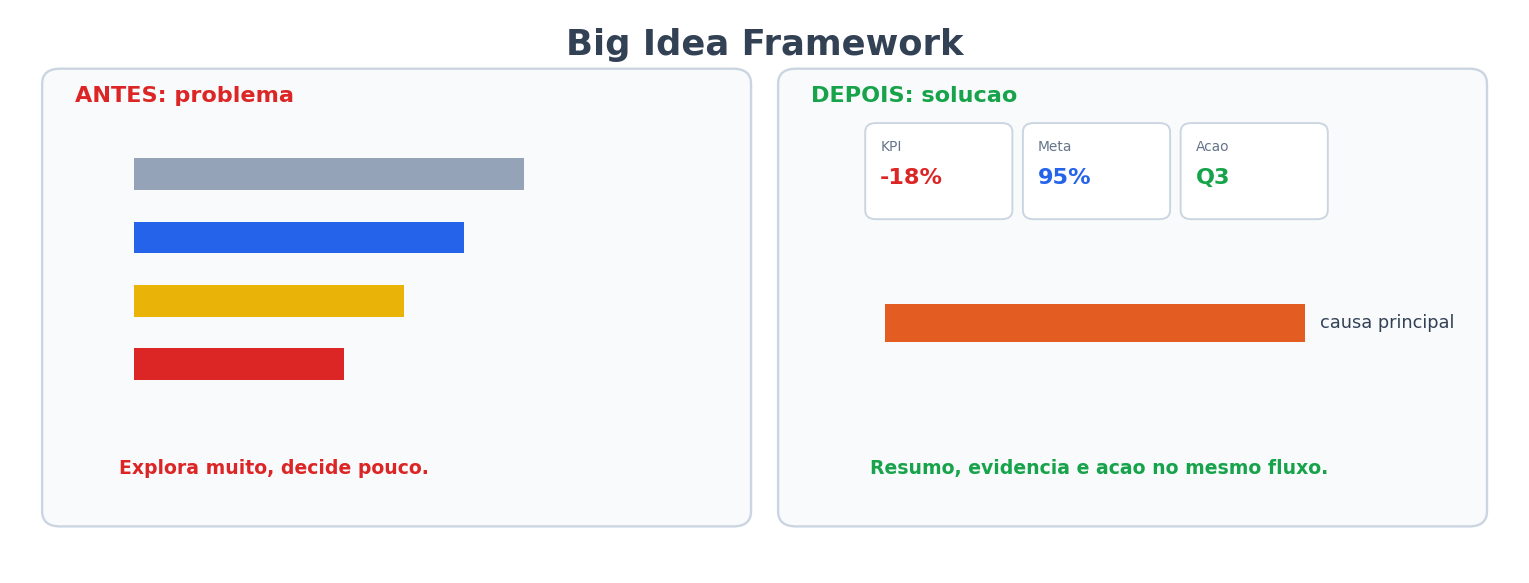
\includegraphics[width=0.58\textwidth]{semana_especial/outputs/cmp_cap2_big_idea.png}
\end{center}

Toda Big Idea está ligada a uma \textbf{pergunta de decisão}: a questão que a audiência precisa responder ao final. Exemplos: ``Devemos expandir para o canal digital ou reforçar o físico?''; ``Qual produto descontinuamos no Q3?''. O analista não precisa ter a resposta --- mas deve apresentar os dados que tornam a resposta possível.

\textbf{Mais exemplos de Big Ideas em diferentes domínios:}
\begin{itemize}
  \item \textit{E-commerce:} ``Frete grátis acima de R\$100 aumenta o ticket médio em 34\%, mas reduz a margem em apenas 8\% --- implementar já seria rentável no Q3.''
  \item \textit{RH:} ``Desenvolvedores sem promoção em 3 anos têm 5$\times$ mais chance de sair; implementar plano de carreira acelerado para 23 talentos preservaria R\$480k em custos de reposição anual.''
  \item \textit{Saúde:} ``Pacientes que recebem chamada de lembrete 24h antes da consulta aumentam a taxa de comparecimento em 41\%; reduz custos operacionais em R\$120k/ano.''
\end{itemize}

\textbf{Teste na prática:} leia sua Big Idea para um colega que não mexe com seus dados. Se ele disser ``muito interessante'', ela ainda não está pronta. Se ele disser ``e quando a gente começa?'', pronto --- você tem uma Big Idea de verdade.

% -------------------------------------------------------
\section{Storyboard e Estrutura Narrativa}
% -------------------------------------------------------

Antes de abrir o Tableau e construir qualquer gráfico, você desenha o \textbf{storyboard} --- um rascunho em papel com os títulos das telas e o tipo de visual em cada uma. Ele força você a pensar na narrativa \emph{antes} de pensar nas ferramentas. Quem abre o Tableau sem storyboard constrói gráficos bonitos sem história.

Nancy Duarte propõe uma estrutura de 4 atos adaptada de narrativas clássicas. O truque é que toda boa apresentação de dados segue exatamente essa ordem: você mostra o estado atual, revela a tensão, apresenta a proposta e termina com um pedido concreto.

\begin{BoardBox}[title=Estrutura Narrativa --- 4 Atos]
\begin{enumerate}
  \item \textbf{Contexto --- O que é:} estado atual; KPIs reais; o ponto de partida.
  \item \textbf{Conflito --- O que poderia ser:} a tensão; o dado que revela o problema.
  \item \textbf{Resolução --- O que proponho:} proposta baseada em evidências.
  \item \textbf{Call to Action:} decisão pedida + responsável + prazo.
\end{enumerate}
\smallskip
\textbf{Em telas:} KPIs atuais \textrightarrow{} problema \textrightarrow{} análise/evidências \textrightarrow{} recomendação
\end{BoardBox}

Cada tela do storyboard deve ter: (1) título que é mensagem --- não ``Gráfico de Barras'', mas sim ``Canal físico custa 4$\times$ mais por venda''; (2) tipo de visual proposto; (3) esboço manual do dado; (4) transição lógica para a próxima tela, como ``por isso, na próxima tela, veja\ldots''

\begin{center}
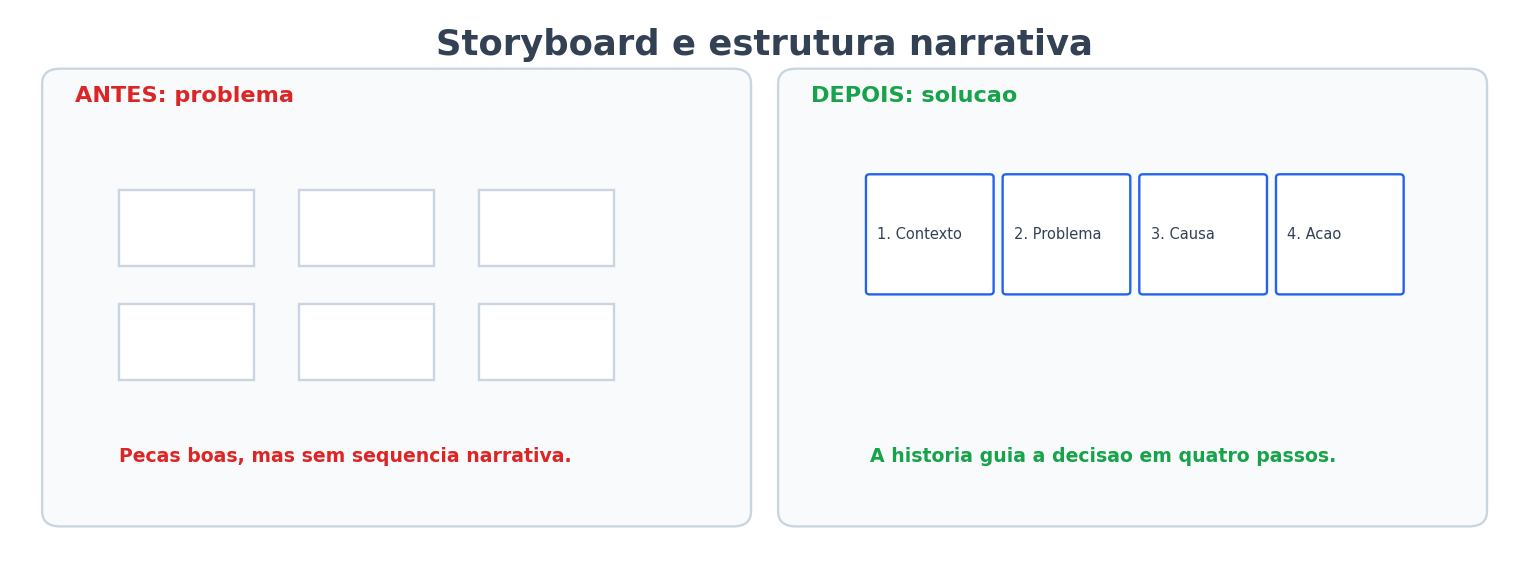
\includegraphics[width=0.58\textwidth]{semana_especial/outputs/cmp_cap2_storyboard.png}
\end{center}

\textbf{Exemplo de storyboard em 4 telas de uma apresentação executiva:}
\begin{enumerate}
  \item \textbf{Tela 1 --- Contexto:} ``Vendas em regiões Sul e Centro-Oeste crescem 15\% acima da média nacional.'' (Big Number destacado + KPI) Transição: ``mas quando olhamos a margem, a história muda radicalmente.''
  \item \textbf{Tela 2 --- Conflito:} ``Essas mesmas regiões têm margem negativa em Tecnologia.'' (Scatter: Desconto vs Margem, cor vermelho no quadrante negativo) Transição: ``achamos 3 subcategorias que concentram 73\% do prejuízo.''
  \item \textbf{Tela 3 --- Análise:} ``Máquinas em SP têm desconto médio de 26\%; Copiadoras em Sul, 23\%; comparando com Nordeste (14\%), o culpado é a política de desconto regional.'' (Tabela + box destacando as 3 categorias críticas) Transição: ``por isso recomendamos\ldots''
  \item \textbf{Tela 4 --- Recomendação:} ``Capar desconto máximo em 12\% em Tecnologia/Sul até 01/junho recupera R\$85k de margem trimestral e move o resultado de -4,2\% para +5,8\%.'' (Simulação com 3 cenários: otimista, realista, pessimista) Próximo passo: ``Gerência Comercial, confirmar a implementação até 15/maio?''
\end{enumerate}

O storyboard em papel \textbf{antes de você abrir o Tableau} economiza semanas de trabalho. Você já sabe qual série temporal é importante, qual drill-down você precisa, quantas telas usará. Quem pula essa etapa muitas vezes constrói um dashboard tecnicamente correto mas narrativamente confuso.

% -------------------------------------------------------
\section{Design de Informação: Pré-atenção e Atributos Visuais}
% -------------------------------------------------------

Antes de você ler deliberadamente qualquer coisa num gráfico, seu cérebro já detectou alguns elementos em menos de 250 milissegundos, sem esforço consciente. Esses são os \textbf{atributos pré-atencionais}. Se você os usa para destacar o que importa, o leitor chega à mensagem antes de ler o título. Se os usa aleatoriamente, o leitor fica desorientado.

A regra de ouro é usar no máximo \textbf{dois atributos pré-atencionais} por visual. Acima disso, a hierarquia colapsa e o olho não sabe onde pousar.

\begin{BoardBox}[title=Atributos Pré-atencionais]
\begin{tabular}{@{}llp{5.2cm}@{}}
\toprule
\textbf{Atributo} & \textbf{Função} & \textbf{Regra de uso} \\
\midrule
Cor        & Destaca, agrupa       & 1 cor de destaque; resto em cinza neutro \\
Tamanho    & Indica magnitude      & Maior = mais importante; consistência obrigatória \\
Posição    & Organiza hierarquia   & Mais importante: canto superior esquerdo \\
Intensidade & Contraste claro/escuro & Mais escuro = mais importante \\
Enclosure  & Agrupa elementos      & Caixa ao redor de dados relacionados \\
\bottomrule
\end{tabular}
\end{BoardBox}

A \textbf{cor} merece atenção especial. Há a cor semântica (vermelho = alerta, verde = ok, amarelo = atenção) e a cor de destaque (uma cor viva para o elemento que carrega a mensagem; todo o resto em cinza). Use cor semântica onde já existe convenção estabelecida. Nunca inverta vermelho e verde sem motivo forte. E lembre: 8\% dos homens têm daltonismo vermelho-verde --- evite que essa combinação seja o único diferenciador.

\begin{center}
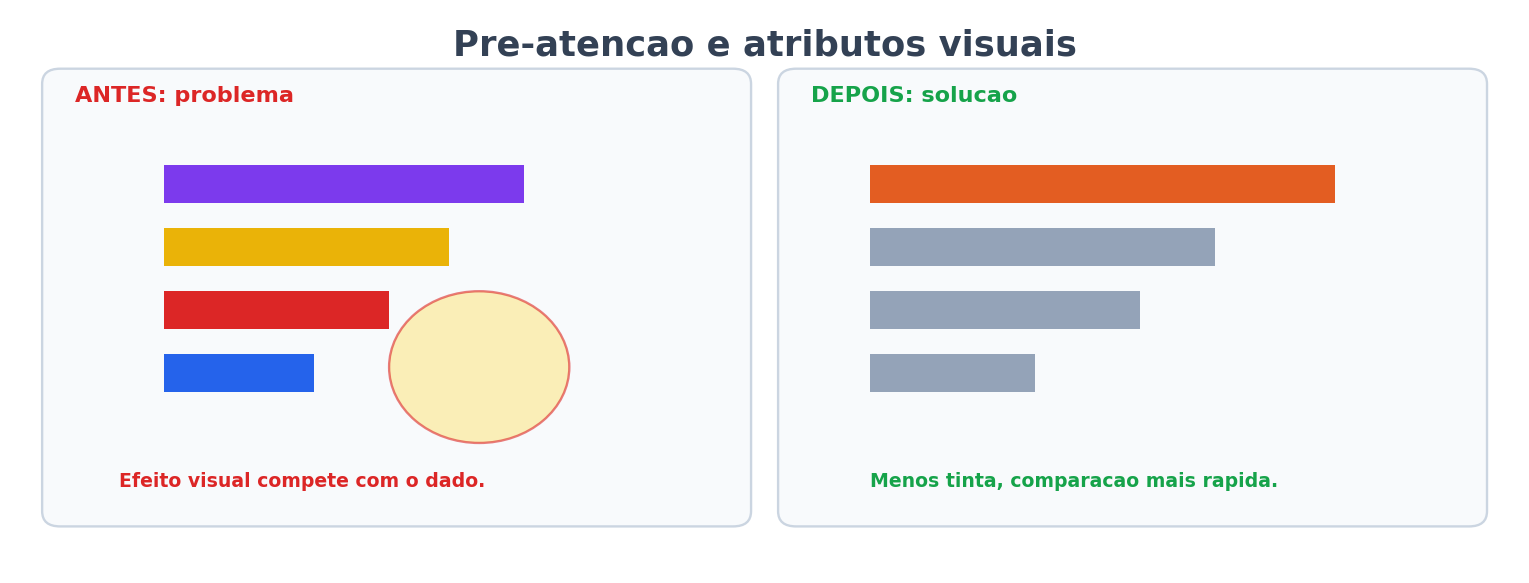
\includegraphics[width=0.58\textwidth]{semana_especial/outputs/cmp_cap2_preatencao.png}
\end{center}

\textbf{Regra de ouro revisitada:} você consegue usar até 2 atributos pré-atencionais em harmonia. Exemplo: na ábaco visual mostrando performance por time, use \textbf{COR} para semântica (verde = meta atingida, vermelho = abaixo) e \textbf{TAMANHO} para magnitude (bolinha grande = time grande, bolinha pequena = time pequeno). Juntos, os dois atributos permitem decodificação instantânea. Se você adicionar um terceiro --- posição espacial não óbvia, ou intensidade de padrão --- o cérebro fica sobrecarregado e falha no teste do relance. Na prática, quando você entra na dúvida de ``será que está confuso?'', sempre está. Remova o terceiro atributo.

% -------------------------------------------------------
\section{Teste do Relance e Título-Mensagem}
% -------------------------------------------------------

O Teste do Relance é simples: mostre o gráfico por 3 segundos, cubra e pergunte à audiência o que viram e qual a mensagem principal. Se não conseguirem responder em 3 segundos, o visual falhou. Não o leitor --- o design.

\begin{BoardBox}[title=Teste do Relance --- Diagnóstico de Falha]
Causas mais comuns de falha:
\begin{itemize}
  \item Título rótulo em vez de título mensagem
  \item Excesso de elementos --- o olho não sabe onde pousar
  \item Cores sem propósito --- todas as barras em cores diferentes
  \item Legenda separada --- o leitor desvia o olhar para decodificar
\end{itemize}
\smallskip
\textbf{Fórmula do título mensagem:} [Sujeito] + [verbo de tendência] + [magnitude]\\
Ex.: ``Churn \textbf{caiu} 34\% após o programa de fidelidade''
\end{BoardBox}

A diferença entre título rótulo e título mensagem é a diferença entre ``Vendas por Região'' e ``Região Sul concentra 58\% das vendas''. O primeiro descreve o que o eixo mostra. O segundo já entrega a informação. Para o executivo com 5 minutos por dia, o título mensagem é o gráfico mais importante --- porque ele consegue ler apenas os títulos e já sabe o que decidir.

\begin{center}
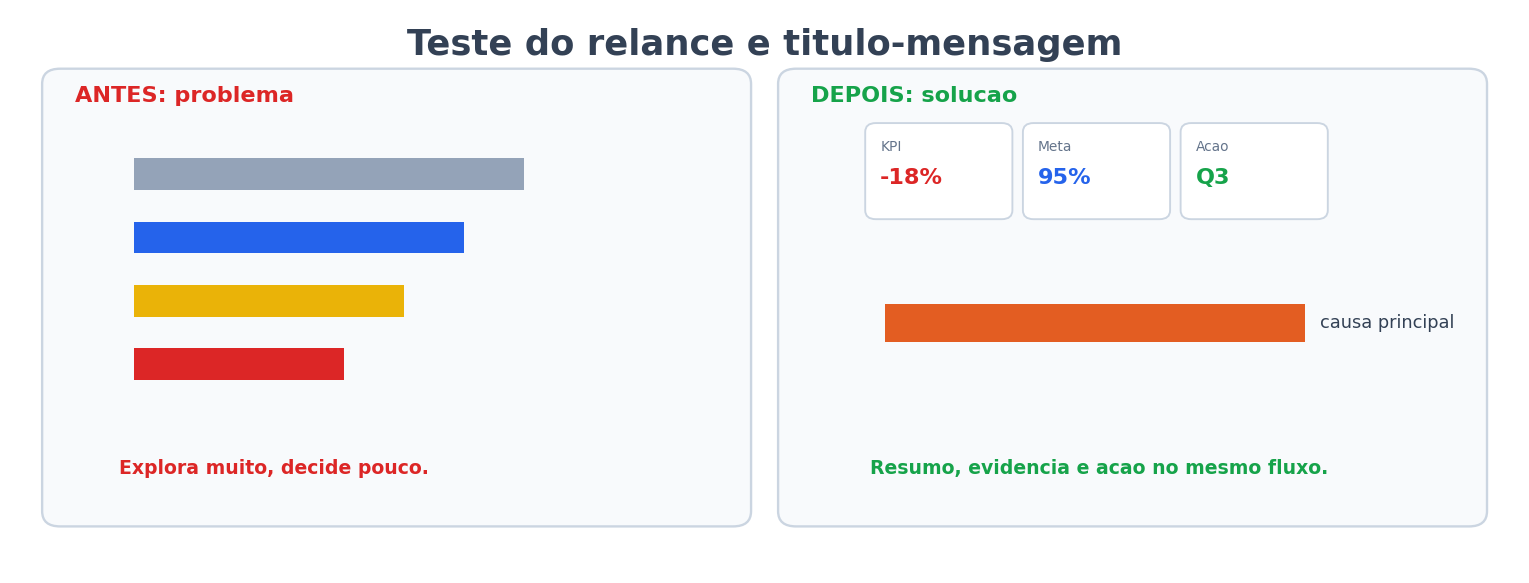
\includegraphics[width=0.58\textwidth]{semana_especial/outputs/cmp_cap2_relance.png}
\end{center}

\textbf{Checklist para passar no Teste do Relance:} (1) título é mensagem, não rótulo? (2) cores comunicam semântica ou prioridade, não decoração? (3) gráfico tem exatamente 1 ou 2 atributos pré-atencionais, não mais? (4) sem ambiguidade: alguém que não viu o dado sabe imediatamente qual a mensagem?

Quando você apresenta um dashboard para alguém pela primeira vez, teste na prática: mostre por 3 segundos, tape a tela e pergunte ``qual a mensagem principal deste gráfico?'' Se a resposta não estiver clara, você ainda tem trabalho. Se estiver absolutamente cristalina --- pronto, passou.

% -------------------------------------------------------
\section{Data-Ink Ratio e Chartjunk}
% -------------------------------------------------------

Edward Tufte (1983) propõe o conceito de \textbf{data-ink ratio}: a proporção da tinta do gráfico que realmente representa dados sobre a tinta total. Maximize esse ratio. Tudo que ocupa tinta sem carregar informação é candidato à remoção.

\begin{BoardBox}[title=Data-Ink Ratio e Chartjunk]
\[
  \text{Data-ink ratio} = \frac{\text{tinta que representa dados}}{\text{tinta total do gráfico}}
\]
\textbf{Chartjunk --- remova:} grades pesadas $\cdot$ barras 3D $\cdot$ sombras $\cdot$ gradientes decorativos $\cdot$ legendas redundantes $\cdot$ ícones temáticos $\cdot$ mais de 3 casas decimais\\[4pt]
\textbf{Princípio:} ``Se eu remover isso, o gráfico fica menos claro?'' Se não --- remova.
\end{BoardBox}

O gráfico de pizza com 8 fatias em 8 cores é o exemplo clássico de chartjunk. O olho humano não compara ângulos com precisão; ele compara comprimentos. Substitua pizza por barras horizontais ordenadas, com 1 cor de destaque para a categoria que carrega a mensagem e rótulos diretos nas barras --- elimine a legenda.

\begin{center}
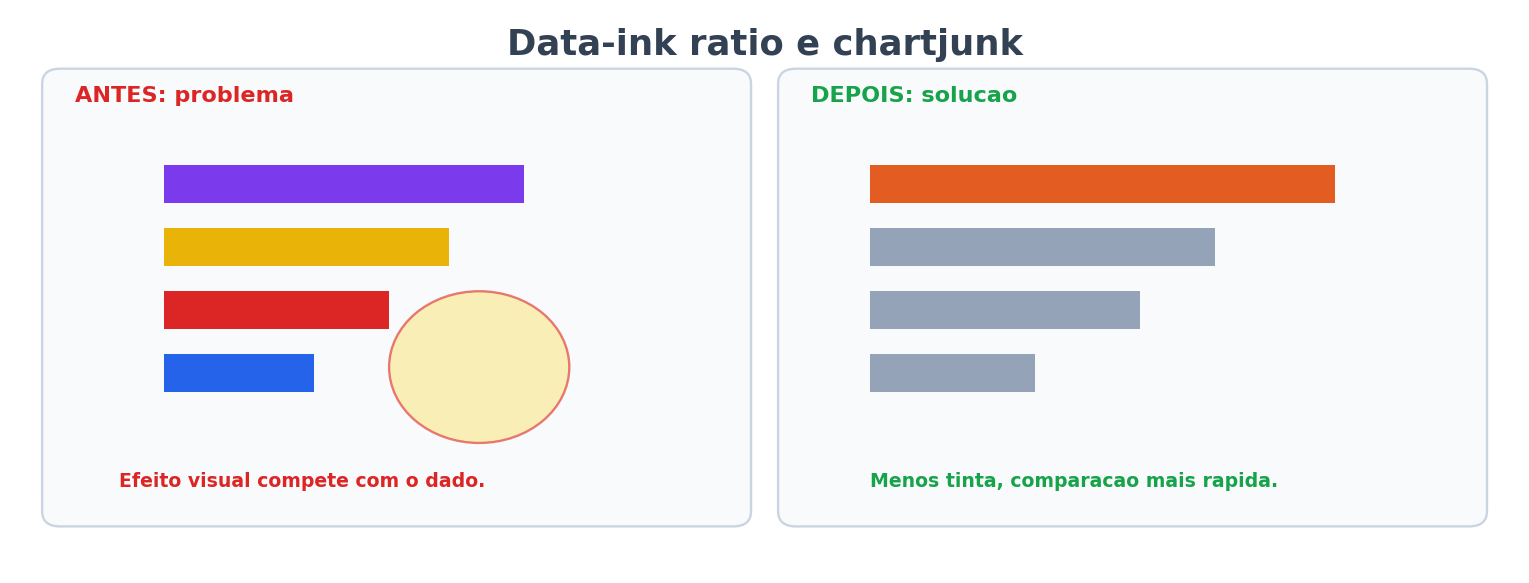
\includegraphics[width=0.58\textwidth]{semana_especial/outputs/cmp_cap2_chartjunk.png}
\end{center}

\textbf{Exemplo de eliminação de chartjunk em 3 passos:} Você tem um gráfico de barras com: (1) grid pesado horizontal e vertical (remove); (2) barras com borda preta (remove); (3) sombra abaixo das barras (remove); (4) legenda no lado dizendo ``Série 1'' (remove --- coloque o rótulo direto na barra); (5) números com 3 casas decimais (reduz para 1 ou 2). Resultado final: data-ink ratio sobe de 50\% para 85\%, o gráfico fica 70\% menor em tamanho visual, e a mensagem fica mais clara.

Em Tableau, a regra é simples: remova toda grid, remova border das marcas, use espaçamento generoso, e ative os rótulos diretos. O resultado é um visual que cabe em uma tela de executivo sem parecer ``deserto''.

% -------------------------------------------------------
\section{Tableau: Filtros, Parâmetros e Ações}
% -------------------------------------------------------

Dois recursos fundamentais de interatividade no Tableau que os alunos frequentemente confundem. A diferença é direta: \textbf{filtros} incluem ou excluem linhas do dataset; \textbf{parâmetros} mudam o cálculo sem filtrar nenhuma linha. Um filtro por estado exibe só os dados de PE --- os dados de SP desaparecem da view. Um parâmetro de métrica permite que o usuário escolha entre Receita ou Margem --- nenhum dado é excluído, apenas o campo calculado muda.

\begin{BoardBox}[title=Filtros vs.\ Parâmetros]
\begin{tabular}{@{}lp{4.5cm}p{5.2cm}@{}}
\toprule
 & \textbf{Filtro} & \textbf{Parâmetro} \\
\midrule
Função   & Inclui/exclui linhas      & Muda o cálculo \\
Uso      & Selecionar região, categoria & Alternar métrica, definir meta, Top N \\
Exemplo  & ``Ver só PE''             & ``Exibir Receita ou Margem?'' \\
\bottomrule
\end{tabular}
\smallskip

\textbf{Campo calculado com parâmetro:}\\
\texttt{IF [Vendas] >= [Meta] THEN ``Atingiu'' ELSE ``Abaixo'' END}
\end{BoardBox}

Sobre a \textbf{hierarquia de filtros}: o Tableau executa filtros em ordem fixa. O mais importante para a prova é o \textbf{Context Filter}. Quando você precisa de Top~N dentro de uma região já filtrada, adicione o filtro de região como Context Filter primeiro --- senão o Tableau calcula o Top~N sobre o dataset inteiro, ignorando o filtro de região.

\begin{center}
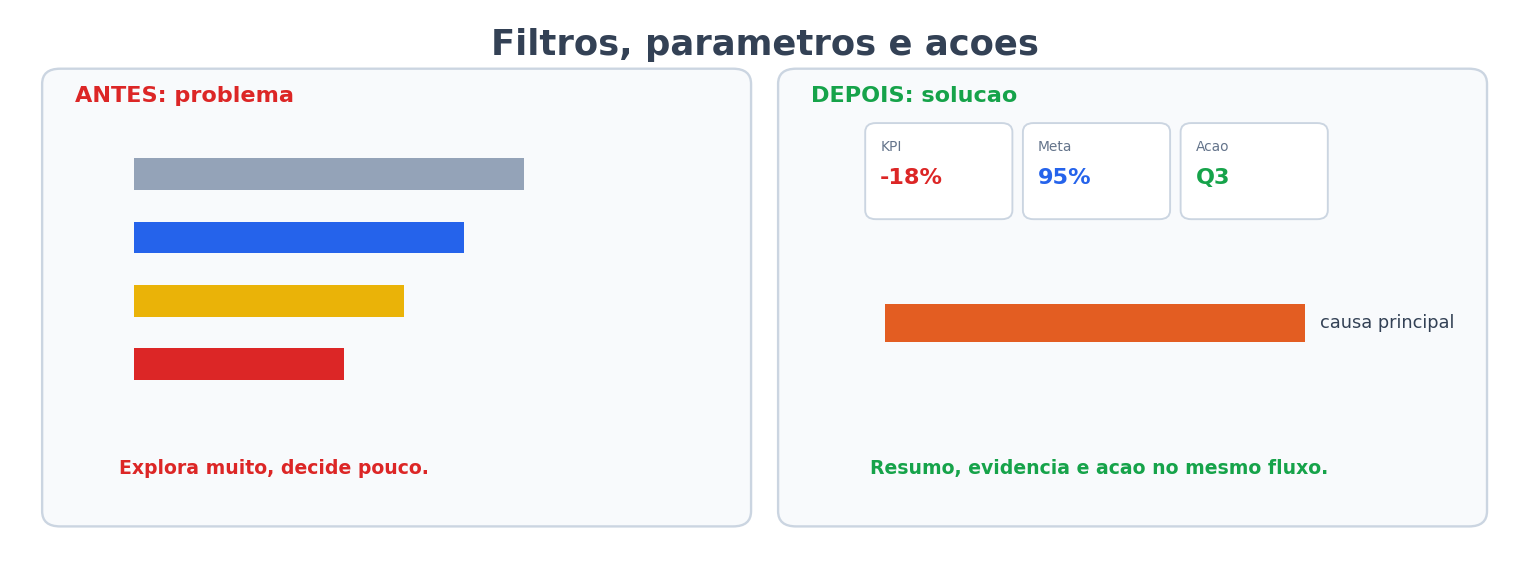
\includegraphics[width=0.58\textwidth]{semana_especial/outputs/cmp_cap2_tableau.png}
\end{center}

\textbf{Pseudocódigo Tableau para parâmetros:} você cria um parâmetro chamado \verb|[Métrica_Selecionada]| com opções ``Receita'', ``Margem'', ``Unidades''. Depois cria um campo calculado:
\begin{quote}\ttfamily
IF [Métrica\_Selecionada] = ``Receita'' THEN [Receita]\\
ELSEIF [Métrica\_Selecionada] = ``Margem'' THEN [Margem]\\
ELSE [Unidades] END
\end{quote}
Quando o usuário muda o parâmetro, o campo calculado avalia instantaneamente e todo o dashboard reflete a mudança. Nenhuma linha é filtrada, apenas o cálculo muda.

\textbf{Context Filter --- quando usar:} você está vendo Top 10 Produtos por Receita em São Paulo. Se você não adicionar ``Estado = SP'' como Context Filter, o Top 10 é calculado sobre TODOS os estados, depois filtrado --- resultado: pode aparecer um produto de outro estado. Com Context Filter, o Top 10 é calculado apenas em SP, garantindo que os 10 maiores de SP apareçam.

\begin{BoardBox}[title=Ações de Dashboard --- 4 Tipos]
\begin{tabular}{@{}lp{4cm}p{4.8cm}@{}}
\toprule
\textbf{Tipo}     & \textbf{O que faz}                  & \textbf{Exemplo} \\
\midrule
Filter action   & Clicar filtra outra view             & Clicar em SP filtra todos os gráficos \\
Highlight       & Destaca sem filtrar                  & Mouse em Região destaca no mapa \\
URL action      & Abre URL com dado selecionado        & Clique abre ficha no ERP \\
Navigate        & Navega entre dashboards              & KPI leva ao painel de drill-down \\
\bottomrule
\end{tabular}
\end{BoardBox}

% -------------------------------------------------------
\section{Dashboards que Forçam Decisão}
% -------------------------------------------------------

Um dashboard pode ser tecnicamente impecável e ainda assim não provocar nenhuma ação. O problema, nesse caso, é de estrutura narrativa. Um dashboard que \textbf{força uma decisão} tem três zonas distintas e em sequência.

\begin{BoardBox}[title=As 3 Zonas do Dashboard Decisório]
\textbf{Zona 1 --- Contexto:} o que está acontecendo agora? KPIs com comparação à meta ou período anterior. Lido em $<$5 segundos. Nenhuma interpretação ainda.

\textbf{Zona 2 --- Diagnóstico:} por que está acontecendo? Drill-down por produto, região, segmento. Permite formular hipóteses --- não confirmar causas.

\textbf{Zona 3 --- Recomendação:} o que fazer? 1--2 recomendações concretas com evidências. Call to Action com \emph{quem}, \emph{o quê} e \emph{até quando}.
\end{BoardBox}

Os \textbf{anti-padrões} mais comuns: (a) tudo sempre verde --- cria conforto falso e impede decisões urgentes; (b) métricas sem definição --- ``Receita'' pode ser bruta, líquida ou MRR, e sem definição explícita cada pessoa lê diferente; (c) 50~KPIs na tela inicial --- granularidade excessiva, o usuário não sabe onde olhar; (d) número isolado sem comparação --- R\$100k de vendas é ótimo ou péssimo em relação ao quê?

\begin{center}
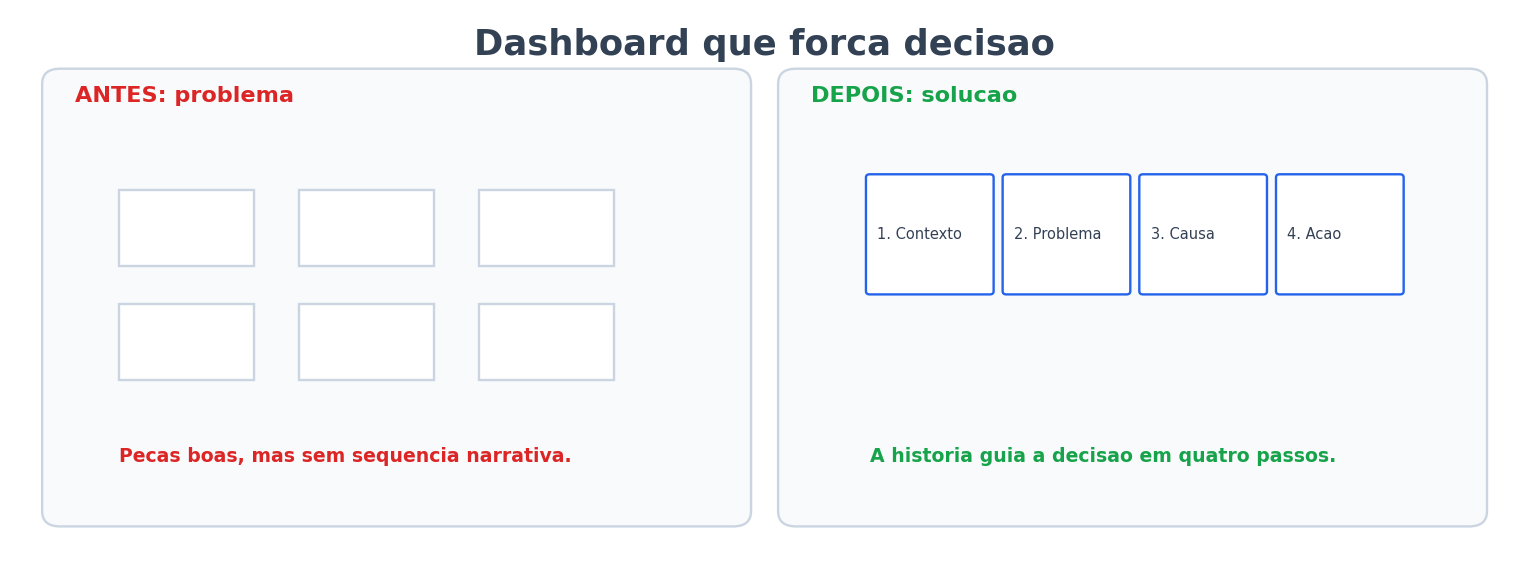
\includegraphics[width=0.58\textwidth]{semana_especial/outputs/cmp_cap2_decisorio.png}
\end{center}

\textbf{Implementação prática das 3 zonas em um dashboard de Vendas:}
\begin{itemize}
  \item \textbf{Zona 1 (Contexto):} 4 KPIs acima da dobra: (1) Receita Mês, Meta, Gap; (2) Margem %; (3) Churn; (4) NPS. Cada KPI mostra ícone de semáforo (verde/amarelo/vermelho). Tempo de leitura: <3 segundos. Nenhuma ação ainda.
  \item \textbf{Zona 2 (Diagnóstico):} 3 gráficos lado a lado: (1) Receita por Região (barras horizontais); (2) Churn vs Desconto (scatter); (3) Série temporal de Margem (linha com meta). Permite que o usuário formule hipóteses (``RJ tem desconto alto demais?'') mas não confirma causas.
  \item \textbf{Zona 3 (Recomendação):} 1 caixa destacada em cor de alerta: ``RJ concentra 65\% da receita mas margem negativa. Reduzir desconto de 26\% para 12\% recupera R\$85k trimestral sem impactar volume (elasticidade = 0,34). Gerência Comercial: implementar até 30/junho.''
\end{itemize}

\textbf{Teste de efetividade:} se seu gerente consegue ler apenas a Zona 3 e já tem uma decisão clara e acionável, sua estrutura funcionou. Se ele precisa voltar para a Zona 2 para entender, significa que a Recomendação não está autossuficiente.

% -------------------------------------------------------
\section{KPIs com Meta, Gap e Tendência}
% -------------------------------------------------------

Um KPI sozinho não decide nada. Para forçar uma decisão, ele precisa de cinco componentes. O número isolado responde ``qual é o valor?'' mas não responde ``isso é bom ou ruim?'' nem ``a situação está melhorando ou piorando?''

\begin{BoardBox}[title=Anatomia de um KPI Decisório]
\begin{enumerate}
  \item \textbf{Valor atual} --- o número real do período
  \item \textbf{Meta (target)} --- o que deveria ser
  \item \textbf{Gap} --- distância em valor absoluto e percentual
  \item \textbf{Tendência} --- seta de alta/baixa ou sparkline
  \item \textbf{Período} --- MTD, YTD, vs ano anterior
\end{enumerate}
\smallskip
\textbf{Bullet chart} (Stephen Few): barra real + barra de meta. Mais informação por cm$^2$ do que qualquer velocímetro ou gauge.
\end{BoardBox}

\begin{center}
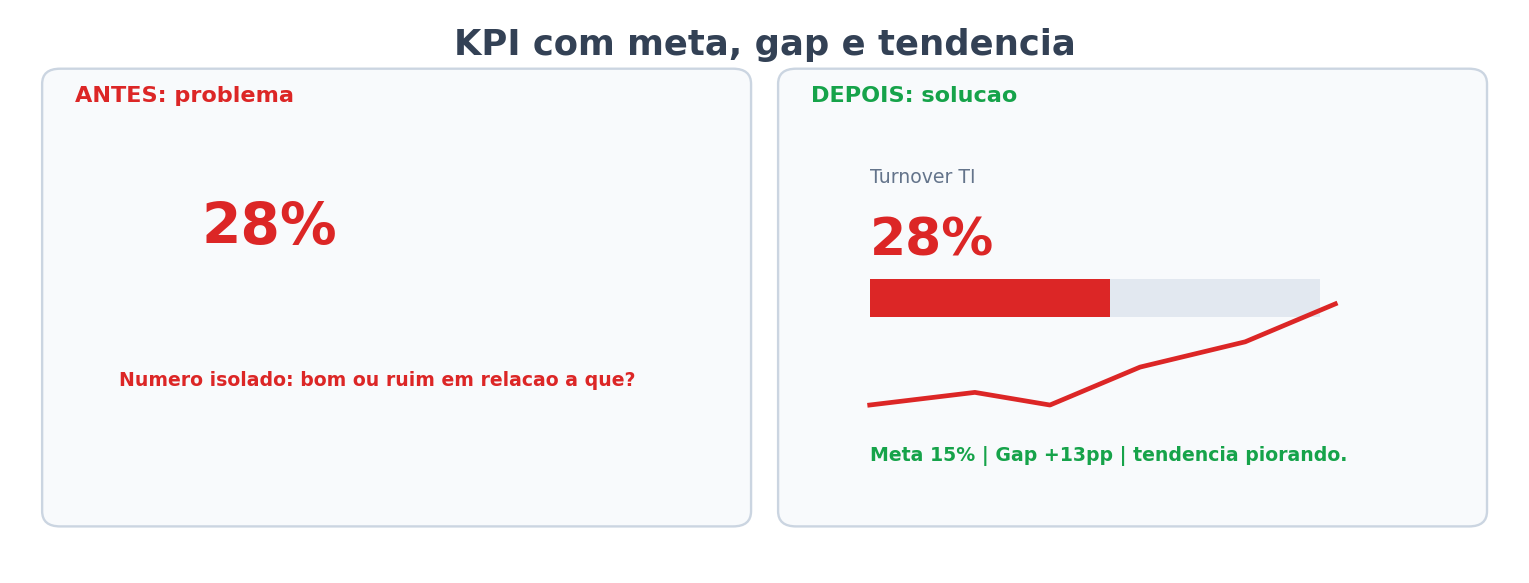
\includegraphics[width=0.58\textwidth]{semana_especial/outputs/cmp_cap2_kpi.png}
\end{center}

\textbf{Exemplos de KPIs bem estruturados em diferentes domínios:}
\begin{itemize}
  \item \textit{E-commerce:} Taxa de Retorno 8\% (Meta: 5\%, Gap: +3pp, Tendência: queda, melhorando, Período: YTD 2026)
  \item \textit{RH:} Turnover TI 28\% (Meta: 15\%, Gap: +13pp, Tendência: alta, piorando, Período: últimos 12 meses)
  \item \textit{Saúde:} Taxa de Readmissão 6,5\% (Meta: 5\%, Gap: +1,5pp, Tendência: alta, piorando, Período: YTD 2026)
\end{itemize}

Quando você tem espaço, a \textbf{bullet chart} (Stephen Few, 2006) é superior ao gauge ou velocímetro porque mostra valor atual, meta, faixa de desempenho bom/médio/ruim, tudo em uma linha horizontal. Se você tiver apenas espaço para um cartão quadrado, use: número grande + meta + gap colorido + sparkline de tendência.

\textbf{Anti-padrão a evitar:} número isolado na tela. Sempre sempre sempre colocar número com: (1) meta ou benchmark; (2) período; (3) tendência. Caso contrário, o número não informa nada --- pode ser bom, ruim, normal. O contexto é o que faz um número virar insight.

% -------------------------------------------------------
\section{Pitch de 3 Minutos}
% -------------------------------------------------------

Três minutos são aproximadamente 450 palavras. Isso é suficiente para convencer alguém --- se e somente se você seguir a estrutura certa. A estrutura SCR (Situação, Complicação, Resolução) tem quatro blocos com tempos definidos.

\begin{BoardBox}[title=Pitch de 3 Minutos --- Estrutura SCR]
\begin{enumerate}
  \item \textbf{Situação (30s):} contexto factual. Comece com o dado impactante, não com introdução genérica.
  \item \textbf{Complicação (45s):} o problema ou oportunidade revelado. Aqui entra a Big Idea.
  \item \textbf{Resolução (60s):} evidência + recomendação com número concreto. Não ``melhorar'' --- sim ``aumentar em 15\%''.
  \item \textbf{Próximo passo (45s):} pedido específico com \textit{verbo + quem + prazo}.
\end{enumerate}
\end{BoardBox}

O erro mais comum: começar com contexto genérico (``vivemos em uma era de dados\ldots'') em vez do dado que mais surpreende. Se você tem 3 minutos e gasta 30 segundos com introdução desnecessária, perdeu 17\% do tempo e a atenção da audiência.

\begin{center}
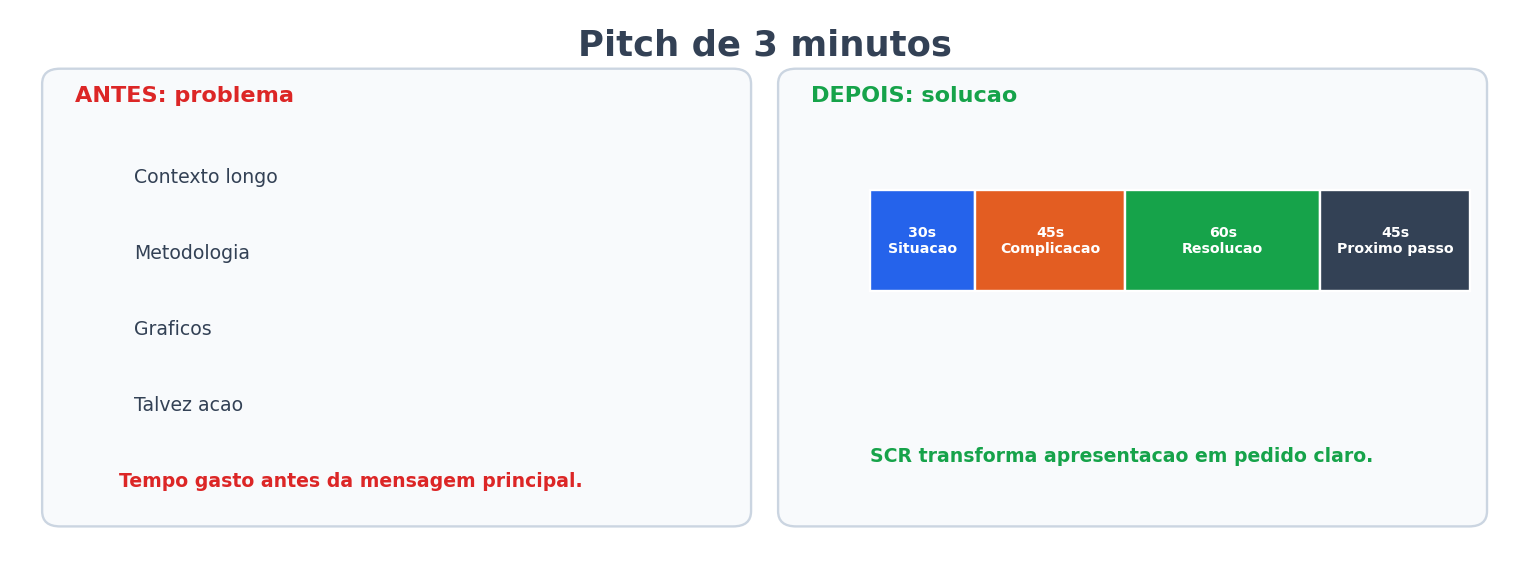
\includegraphics[width=0.58\textwidth]{semana_especial/outputs/cmp_cap2_pitch.png}
\end{center}

\textbf{Exemplo de pitch de 3 minutos em contexto acadêmico:}\\[2pt]
\textbf{Situação (30s):} ``6.607 alunos. 27\% têm nota final menor que 60. Isso significa 1.800 alunos em recuperação, triplicando a carga administrativa e reduzindo a taxa de aprovação final.''\\[2pt]
\textbf{Complicação (45s):} ``Descobrimos que esses alunos compartilham um perfil comum: envolvimento familiar baixo, menos de 15 horas de estudo por semana, e sem ninguém fazendo mentoria. A consequência é uma defasagem de 9 pontos na nota média desse grupo. Se nada mudar, estaremos triplicando esforço e mantendo o mesmo resultado.''\\[2pt]
\textbf{Resolução (60s):} ``Implementamos um programa piloto de mentoria + comunicação familiar com 220 desses alunos em 2025. Resultado: 40\% desse grupo passou a atingir nota acima de 60, aumentando a taxa de aprovação em 8pp e reduzindo custos operacionais de recuperação em R\$45k por ciclo.''\\[2pt]
\textbf{Próximo passo (45s):} ``Recomendo ampliar o programa para todos os alunos em risco (1.800 alunos) no próximo semestre. Implementação começa em julho, com coordenação com coordenação acadêmica. Impacto projetado: +12pp na taxa de aprovação e economia sustentável de R\$120k/ano.''

\textbf{Timing checklist:} você praticou em voz alta? Esse é o teste final. Textos parecem curtos quando lidos mentalmente; no palco, correm 40\% mais rápido do que você pensa. Se você não praticar, vai acabar rápido demais e sobrar tempo, ou vai ficar atropelado tentando terminar em 3 minutos.

% ============================================================
\section*{\Large PARTE II --- QUESTÕES DAS PROVAS --- UNIDADE II}
% ============================================================

As questões abaixo estão no formato exato das provas. \textbf{Prova II Unidade} primeiro (5 questões de 2,0 pts cada). Depois as questões de Unidade~II da \textbf{Prova Final} (Q8, Q9 e Q10 --- 1,0 pt cada). Por fim as questões de Unidade~II da \textbf{Prova II Chamada} (Q8, Q9 e Q10 --- 1,0 pt cada). Os cenários foram levemente adaptados para fins didáticos.

% ============================================================
\subsection*{Prova II Unidade (5 questões $\times$ 2,0 pts)}
% ============================================================

% --- Q1 --- Big Idea
Beatriz é analista de dados em uma rede de 18 farmácias no Recife. Ela foi solicitada a apresentar os resultados de sua análise sobre cancelamentos do programa de fidelidade para a reunião trimestral de diretoria. Após semanas de análise exploratória, Beatriz descobriu que: 72\% dos cancelamentos ocorrem nos primeiros 2 meses; clientes que resgatam pelo menos 1 benefício no primeiro mês têm 80\% de chance de permanecer; o canal de cadastro via WhatsApp tem taxa de retenção 35\% maior que o cadastro em loja; filas no caixa durante o almoço (12h--13h) estão com tempo médio de 8 minutos, gerando reclamações. Beatriz precisa que a diretoria tome uma decisão clara ao final da apresentação.

\begin{SolvedBox}[title=Questão 1 --- Prova II Unidade (2{,}0 pts) --- Big Idea]
Qual alternativa apresenta a \textbf{Big Idea bem formulada} que Beatriz poderia usar?
\begin{enumerate}[label=\Alph*)]
  \item ``Devemos implementar um fluxo de engajamento automático via WhatsApp nos primeiros 2 meses, com nudge para o primeiro resgate, pois isso pode reduzir cancelamentos em até 55\% e aumentar a receita recorrente do programa em R\$220 mil/ano.''
  \item ``Os dados mostram várias informações interessantes sobre o programa de fidelidade.''
  \item ``Analisamos 22.000 registros de clientes do programa entre 2024 e 2025.''
  \item ``A taxa de cancelamento do programa é de 28\% ao ano.''
  \item ``O gráfico de barras mostra a distribuição de cancelamentos por mês.''
\end{enumerate}
\end{SolvedBox}

\textbf{Gabarito: A.} A alternativa A combina os três elementos obrigatórios: (1) ponto de vista --- ``devemos implementar'' é recomendação de ação, não observação passiva; (2) tensão --- 72\% de cancelamentos nos primeiros 2 meses revela a oportunidade desperdiçada; (3) stake financeiro --- R\$220 mil/ano é o argumento decisivo para a diretoria. B é vaga; C é puramente descritiva; D é um número isolado sem orientação; E é rótulo de gráfico sem valor decisório.

\medskip

% --- Q2 --- Design de Dashboard
Rafael é analista de BI em uma rede varejista de eletrodomésticos com 35 lojas. O diretor comercial tem apenas 5 minutos por dia para ver o dashboard. Rafael está decidindo entre duas abordagens de design. \textbf{Opção A:} título ``Vendas Jan/2026: meta superada em 18\% --- foco em Linha Branca''; KPI central ``118\%'' em verde; barras horizontais com a categoria líder destacada em azul escuro; fundo branco, máx.\ 3 cores com propósito, espaço em branco generoso. \textbf{Opção B:} título ``Dashboard Comercial''; 15 gráficos de tipos variados; todas as 8 cores da paleta utilizadas; sem espaço em branco; títulos genéricos ``Gráfico 1'', ``Gráfico 2''.

\begin{SolvedBox}[title=Questão 2 --- Prova II Unidade (2{,}0 pts) --- Design de Dashboard]
Considerando hierarquia visual e Teste do Relance, qual alternativa avalia \textbf{corretamente} as duas opções?
\begin{enumerate}[label=\Alph*)]
  \item A Opção A é superior: título comunica a mensagem com dado concreto, uso restrito de cores direciona a atenção ao que importa, espaço em branco organiza a hierarquia visual, e o dashboard passa no Teste do Relance.
  \item A Opção B é superior porque tem mais gráficos e mais cores, transmitindo mais informação ao diretor.
  \item Ambas são equivalentes em eficácia comunicativa --- o que importa é o dado, não o design.
  \item A Opção A é inferior porque desperdiça espaço que poderia ter mais gráficos.
  \item Títulos como ``Dashboard Comercial'' são mais profissionais e neutros que títulos com dados.
\end{enumerate}
\end{SolvedBox}

\textbf{Gabarito: A.} A Opção A aplica: título-mensagem com dado concreto e relevância imediata; cor de destaque única para guiar o olho; data-ink ratio maximizado sem chartjunk. A Opção B viola todos os princípios: título rótulo que não informa nada; 15 gráficos fragmentam a atenção; 8 cores sem propósito semântico violam o limite atencional; títulos genéricos que não entregam nenhuma mensagem.

\medskip

% --- Q3 --- Filtros e Parâmetros
Marcos é analista de dados em uma rede de 25 concessionárias de veículos no Nordeste. A gerência pediu que o dashboard permitisse: (1) ver apenas as concessionárias de um estado específico; (2) escolher o período de análise entre mês, trimestre ou semestre; (3) alternar a métrica exibida entre Unidades Vendidas e Receita Total. Marcos precisa decidir quais recursos do Tableau usar para cada necessidade.

\begin{SolvedBox}[title=Questão 3 --- Prova II Unidade (2{,}0 pts) --- Tableau: Filtros e Parâmetros]
Qual alternativa apresenta \textbf{corretamente} o recurso do Tableau para cada necessidade?
\begin{enumerate}[label=\Alph*)]
  \item Filtro para selecionar o estado; Parâmetro para o período (campo calculado ajusta a granularidade de datas); Parâmetro para alternar a métrica (\texttt{IF [Métrica]=``Receita'' THEN [Receita] ELSE [Unidades] END}).
  \item Criar 25 dashboards separados, um para cada concessionária, e deixar o gerente escolher qual abrir.
  \item Usar apenas filtros para as 3 necessidades, sem nenhum parâmetro no dashboard.
  \item Exportar os dados para o Excel e calcular os recortes manualmente cada semana.
  \item Usar apenas parâmetros para todas as 3 necessidades, sem nenhum filtro.
\end{enumerate}
\end{SolvedBox}

\textbf{Gabarito: A.} (1) Filtrar por estado é inclusão/exclusão de linhas --- responsabilidade do Quick Filter. (2) Escolher período envolve cálculo de datas dinâmico que só um Parâmetro + campo calculado resolve. (3) Alternar entre Unidades e Receita muda qual campo é calculado, não filtra linhas --- exclusividade do Parâmetro. C está errado porque filtros não trocam campos calculados; E está errado porque parâmetros não excluem linhas do dataset.

\medskip

% --- Q4 --- Dashboard Decisório
Helena é diretora de expansão de uma plataforma de cursos online e precisa apresentar para o board se deve lançar operações presenciais em Caruaru. Ela estruturou o dashboard em 3 seções. \textbf{Seção 1 --- Contexto:} mapa comparando Recife e Caruaru; indicadores de mercado: população-alvo, renda per capita, taxa de adoção de smartphones. \textbf{Seção 2 --- Diagnóstico:} CAC estimado, LTV projetado, taxa de adoção de plataformas similares na região, análise de concorrência local. \textbf{Seção 3 --- Recomendação:} simulação de payback com cenários otimista, realista e pessimista; call-to-action: ``Caruaru --- lançamento Q3/2026, investimento R\$350k, ROI projetado em 18 meses''. O board tomou a decisão em 10 minutos.

\begin{SolvedBox}[title=Questão 4 --- Prova II Unidade (2{,}0 pts) --- Dashboard Decisório]
Qual alternativa explica \textbf{corretamente} por que a estrutura de Helena foi eficaz?
\begin{enumerate}[label=\Alph*)]
  \item O framework Contexto$\to$Diagnóstico$\to$Recomendação funciona porque estabelece o cenário, evidencia a oportunidade e finaliza com ação concreta; os 3 cenários reduzem incerteza; o call-to-action com prazo e ROI torna a decisão acionável.
  \item O dashboard foi eficaz apenas porque tinha gráficos visualmente bonitos e coloridos.
  \item A ordem das 3 seções é irrelevante; qualquer estrutura funcionaria da mesma forma.
  \item Dashboards não devem incluir recomendações; devem apenas mostrar os dados brutos.
  \item O board tomou a decisão rápido porque não leu o dashboard com atenção suficiente.
\end{enumerate}
\end{SolvedBox}

\textbf{Gabarito: A.} A estrutura em 3 zonas replica o processo de decisão humano. O Contexto cria urgência com dados reais sem parecer alarmismo. O Diagnóstico fecha as dúvidas sobre causa raiz (CAC, LTV, adoção). A Recomendação com 3 cenários + ROI + prazo transforma uma apresentação informativa em um dashboard que \emph{força} a decisão. Sem a Zona~3, o board sai da reunião com dados mas sem clareza de ação.

\medskip

% --- Q5 --- Pitch de 3 minutos
Bruno foi selecionado para apresentar sua análise sobre desnutrição infantil no Sertão de Pernambuco em uma competição de dados. Ele tinha apenas 3 minutos. \textbf{Minuto 1 --- Situação:} ``8.200 crianças abaixo de 5 anos apresentam desnutrição moderada ou grave no Agreste/Sertão. Isso representa R\$1,1 bilhão em impacto econômico projetado até 2035. Nossa análise identificou 3 preditores principais.'' \textbf{Minuto 2 --- Complicação:} visual 1 (mapa de calor dos municípios críticos); visual 2 (correlação renda familiar $\times$ índice nutricional); insight: ``crianças em municípios sem CRAS ativo têm 3,5$\times$ mais risco de desnutrição grave''. \textbf{Minuto 3 --- Resolução:} ``Reativar os 12 CRAS desativados pode reduzir a desnutrição em 32\% em 3 anos. Próximo passo: piloto em 3 municípios no 2º semestre com orçamento de R\$480k.'' Bruno termina dentro do tempo e os jurados compreendem claramente a proposta.

\begin{SolvedBox}[title=Questão 5 --- Prova II Unidade (2{,}0 pts) --- Pitch de 3 Minutos]
Qual alternativa descreve \textbf{corretamente} os elementos que tornaram o pitch de Bruno eficaz?
\begin{enumerate}[label=\Alph*)]
  \item O pitch foi eficaz porque: começou com dado impactante (não com contexto genérico); usou apenas 2 visuais estratégicos, sem sobrecarregar; traduziu o insight em ação concreta com métrica de impacto; e terminou com próximo passo com verbo, quantidade e prazo.
  \item O pitch foi eficaz apenas porque durou exatamente 3 minutos, independente do conteúdo.
  \item Bruno deveria ter mostrado todas as visualizações criadas durante a análise exploratória.
  \item Pitches de dados não devem ter gancho emocional; devem começar direto com tabelas de dados.
  \item A recomendação final é desnecessária; os jurados deveriam decidir sozinhos o que fazer com os dados.
\end{enumerate}
\end{SolvedBox}

\textbf{Gabarito: A.} O pitch de Bruno aplica a estrutura SCR com precisão. A Situação começa com dado quantificado (não introdução genérica). A Complicação usa 2 visuais estratégicos (respeita a capacidade atencional) e entrega o insight com magnitude (3,5$\times$). A Resolução tem percentual de impacto (32\%) e o próximo passo tem os 3 elementos de um call-to-action eficaz: verbo (``reativar''), quantidade (12 CRAS / 3 municípios) e prazo (2º semestre).

% ============================================================
\subsection*{Prova Final --- Unidade II (Q8, Q9 e Q10 --- 1,0 pt cada)}
% ============================================================

As questões Q1 a Q7 da Prova Final cobrem Unidade~I (dicionário de dados, qualidade, médias, desvio-padrão, boxplot, dados ausentes e correlação). As três abaixo são as de Unidade~II.

% --- Final Q8
\begin{SolvedBox}[title=Questão 8 (Prova Final) --- Big Idea (1{,}0 pt)]
Qual frase representa uma \textbf{Big Idea bem formulada} para uma apresentação à diretoria?
\begin{enumerate}[label=\Alph*)]
  \item ``Devemos implantar bônus de permanência nos 2 primeiros anos de empresa, pois a análise mostra redução de 40\% no turnover e economia de R\$180k em custos de reposição de pessoal.''
  \item ``O gráfico de linhas mostra a evolução do turnover por trimestre.''
  \item ``Analisamos 10.000 registros de colaboradores no período de 2023 a 2025.''
  \item ``Os dados de recursos humanos são interessantes e apresentam padrões relevantes.''
  \item ``Tabela 1: distribuição de turnover por departamento e nível hierárquico.''
\end{enumerate}
\end{SolvedBox}

\textbf{Gabarito: A.} A alternativa A tem ponto de vista (``devemos implantar''), tensão (turnover elevado gerando custo de reposição) e stake financeiro concreto (R\$180k). As demais são rótulos de visual (B, E), descrições genéricas (C) ou afirmações sem orientação de ação (D).

% --- Final Q9
\begin{SolvedBox}[title=Questão 9 (Prova Final) --- Design de Dashboard (1{,}0 pt)]
Qual prática é \textbf{recomendada} para criar um dashboard executivo eficaz?
\begin{enumerate}[label=\Alph*)]
  \item Títulos que comunicam a mensagem com dado concreto, uso máximo de 3 cores com propósito semântico, e espaço em branco para organizar a hierarquia visual.
  \item Usar todas as cores disponíveis na paleta para tornar o dashboard visualmente mais atrativo.
  \item Colocar o máximo de gráficos possível para demonstrar todo o trabalho analítico realizado.
  \item Eliminar completamente o espaço em branco para aproveitar toda a área disponível na tela.
  \item Usar títulos genéricos como ``Gráfico 1'' para não influenciar a interpretação do leitor.
\end{enumerate}
\end{SolvedBox}

\textbf{Gabarito: A.} Os princípios de design estabelecem: (a) título-mensagem entrega a informação antes de qualquer leitura do gráfico; (b) máx.\ 3 cores com propósito semântico respeita o limite atencional (mais de 6 cores e o leitor perde a associação cor-categoria); (c) espaço em branco não é desperdício --- é o organizador silencioso da hierarquia visual (leitura em Z).

% --- Final Q10
\begin{SolvedBox}[title=Questão 10 (Prova Final) --- Tableau: Filtros e Parâmetros (1{,}0 pt)]
No Tableau, qual recurso permite que o usuário ajuste \textbf{dinamicamente} uma meta de vendas e o dashboard atualize automaticamente a comparação de desempenho de cada região?
\begin{enumerate}[label=\Alph*)]
  \item Parâmetro combinado com campo calculado que usa o valor do parâmetro como referência.
  \item Exportar o relatório para PDF e recalcular os comparativos manualmente.
  \item Imprimir o dashboard e atualizar os números com caneta a cada nova meta.
  \item Copiar os dados para o Excel e usar PROCV para comparar com a meta.
  \item Usar apenas gráficos estáticos com os dados fixos do período selecionado.
\end{enumerate}
\end{SolvedBox}

\textbf{Gabarito: A.} O parâmetro é um valor dinâmico controlado pelo usuário que pode ser referenciado em qualquer campo calculado. No campo \texttt{IF SUM([Vendas]) >= [Meta] THEN ``Atingiu'' ELSE ``Abaixo'' END}, o usuário ajusta a meta em tempo real e o indicador atualiza instantaneamente. O filtro não faz isso porque inclui/exclui linhas, não altera cálculos.

% ============================================================
\subsection*{Prova II Chamada --- Unidade II (Q8, Q9 e Q10 --- 1,0 pt cada)}
% ============================================================

A Prova II Chamada cobre todo o semestre. As questões Q1 a Q7 são de Unidade~I. As três abaixo são as de Unidade~II.

% --- II Chamada Q8
Uma analista de microcrédito rural trabalha com 30.000 contratos de agricultores no Sertão de PE. Ela identificou: inadimplência geral de 14\% ao ano; clientes sem visita de agente nos últimos 60 dias têm 38\% de inadimplência; clientes com histórico de microcrédito renovado têm apenas 6\% de inadimplência; custo de captação de novo cliente: R\$380.

\begin{SolvedBox}[title=Questão 8 (Prova II Chamada) --- Big Idea (1{,}0 pt)]
Qual alternativa representa a \textbf{melhor Big Idea} para apresentar ao comitê de crédito?
\begin{enumerate}[label=\Alph*)]
  \item ``Devemos implantar visita de agente a cada 45 dias para clientes sem contato recente, pois isso pode reduzir a inadimplência de 38\% para aproximadamente 6\%, economizando R\$210 mil/ano em perdas e evitando R\$380 por cliente em custos de reposição.''
  \item ``A inadimplência do portfólio é de 14\% ao ano.''
  \item ``Analisamos 30.000 contratos de microcrédito ao longo de 18 meses de operação.''
  \item ``Clientes inadimplentes existem por vários motivos e o cenário é complexo.''
  \item ``O gráfico de linhas mostra a tendência de inadimplência nos últimos 24 meses.''
\end{enumerate}
\end{SolvedBox}

\textbf{Gabarito: A.} Mesma lógica: ponto de vista (``devemos implantar'') + dado concreto que cria urgência (38\% vs 6\%) + impacto financeiro quantificado (R\$210k + R\$380/cliente). As demais são vagas, descritivas ou apenas números sem orientação de ação.

% --- II Chamada Q9
\begin{SolvedBox}[title=Questão 9 (Prova II Chamada) --- Título-Mensagem e Teste do Relance (1{,}0 pt)]
Um dashboard executivo precisa mostrar se a meta de vendas foi atingida no trimestre. Qual título de gráfico é \textbf{mais eficaz} segundo o princípio do Teste do Relance?
\begin{enumerate}[label=\Alph*)]
  \item ``Meta superada: Vendas de R\$2,3M excedem a meta de R\$2,0M em 15\%''
  \item ``Dashboard de Vendas Q4''
  \item ``Gráfico 1: Desempenho Comercial''
  \item ``Análise Trimestral de Resultados''
  \item ``Dados de Performance do Período''
\end{enumerate}
\end{SolvedBox}

\textbf{Gabarito: A.} A alternativa A é o único título-mensagem: traz o sujeito (vendas), o verbo de resultado (``superada''), a magnitude (R\$2,3M vs R\$2,0M) e o delta percentual (15\%). Em 3 segundos de relance, o leitor já sabe o resultado sem precisar ler o gráfico. As demais alternativas são todos títulos rótulo: descrevem o tipo ou o período do gráfico, mas não entregam nenhuma informação.

% --- II Chamada Q10
\begin{SolvedBox}[title=Questão 10 (Prova II Chamada) --- Tableau: Ação de Filtro (1{,}0 pt)]
Um analista construiu um dashboard no Tableau. Ele quer que ao clicar em uma barra de um gráfico de vendas por região, um segundo gráfico no mesmo dashboard mostre automaticamente os detalhes daquela região. Qual recurso do Tableau realiza isso?
\begin{enumerate}[label=\Alph*)]
  \item Ação de Filtro (Filter Action): uma seleção em uma visualização filtra outra visualização do mesmo dashboard.
  \item Exportar o dashboard para PDF e criar versões separadas por região manualmente.
  \item Criar 10 dashboards diferentes, um para cada região, e publicar todos no Tableau Public.
  \item Usar apenas parâmetros sem configurar nenhuma ação de dashboard.
  \item Formatação condicional de células no estilo planilha.
\end{enumerate}
\end{SolvedBox}

\textbf{Gabarito: A.} A Filter Action é exatamente o mecanismo de interatividade entre sheets em um dashboard Tableau. Ao configurar: Source Sheet (gráfico de regiões) $\to$ Target Sheet (gráfico de detalhe) $\to$ Trigger: Select, o clique em qualquer barra regional passa o valor selecionado como filtro para a view de destino, atualizando-a instantaneamente. É o recurso mais usado em drill-down de dashboards.

% ============================================================
\section*{\Large PARTE III --- APRESENTAÇÃO EM GRUPO (18/05/2026)}
% ============================================================

% -------------------------------------------------------
\section{Dinâmica, Regras e Estrutura}
% -------------------------------------------------------

Na aula de 18 de maio cada grupo apresenta seu dashboard construído no Tableau durante a própria aula. Este material foi entregue em 04/05 para que cada grupo tenha 14 dias de preparo. O link do Tableau Public deve ser enviado no chat antes de a apresentação começar --- o professor testa ao vivo. O tempo de apresentação é 3 minutos de pitch + 2 minutos de perguntas da turma.

A estrutura obrigatória do dashboard é: \textbf{Pergunta de negócio} $\to$ \textbf{Big Number} (coluna esquerda) + \textbf{Insight gerado por IA} (coluna direita) $\to$ \textbf{Gráficos que respondem à pergunta} $\to$ \textbf{Próxima pergunta} $\to$ \textbf{Gráficos} $\to$ \textbf{Tabela analítica final} (largura total). O Call to Action aparece como título do dashboard ou painel de texto no rodapé.

\begin{BoardBox}[title=Boas Práticas Obrigatórias no Dashboard]
\begin{enumerate}
  \item \textbf{Cor com propósito:} 1 cor de destaque; resto em cinza. Sem arco-íris.
  \item \textbf{Título-mensagem em cada gráfico:} não ``Gráfico de Barras'' --- sim ``X lidera com 2,4$\times$ mais que a média''.
  \item \textbf{Big Number:} fonte $\geq$ 24pt, rótulo descritivo abaixo, indicador de gap com direção + delta.
  \item \textbf{Insight IA:} painel de texto ao lado do Big Number, entre aspas, com rótulo \textbf{[Insight IA]}.
  \item \textbf{Tabela analítica final:} dados consolidados para quem quiser o detalhe.
  \item \textbf{$\geq$ 1 filtro ou parâmetro} funcionando --- dashboard não pode ser puramente estático.
\end{enumerate}
\end{BoardBox}

Enquanto um grupo apresenta, os demais anotam em papel: (1) Big Idea em 1 frase do que ouviram; (2) uma decisão que tomariam com base no dashboard; (3) uma sugestão de melhoria. Isso exercita escuta ativa e gera feedback de valor para o apresentador.

\begin{BoardBox}[title=Prompt para Gerar o Insight IA (ChatGPT ou Gemini)]
\begin{quote}
\small\textit{``Você é analista de dados sênior especializado em [ÁREA DO NEGÓCIO]. Com base nos dados abaixo, gere UM insight acionável em até 3 linhas: (1) padrão não óbvio, (2) impacto quantificado com número concreto, (3) ação específica com estimativa de resultado. Contexto do negócio: [DOR DO GRUPO EM 1 FRASE]. Dados: [COLE O RESUMO DA TABELA ANALÍTICA]. Formato: 1 frase entre aspas, iniciando com o dado mais impactante.''}
\end{quote}
\end{BoardBox}

% -------------------------------------------------------
\section{Grupos e Briefings}

\begin{center}
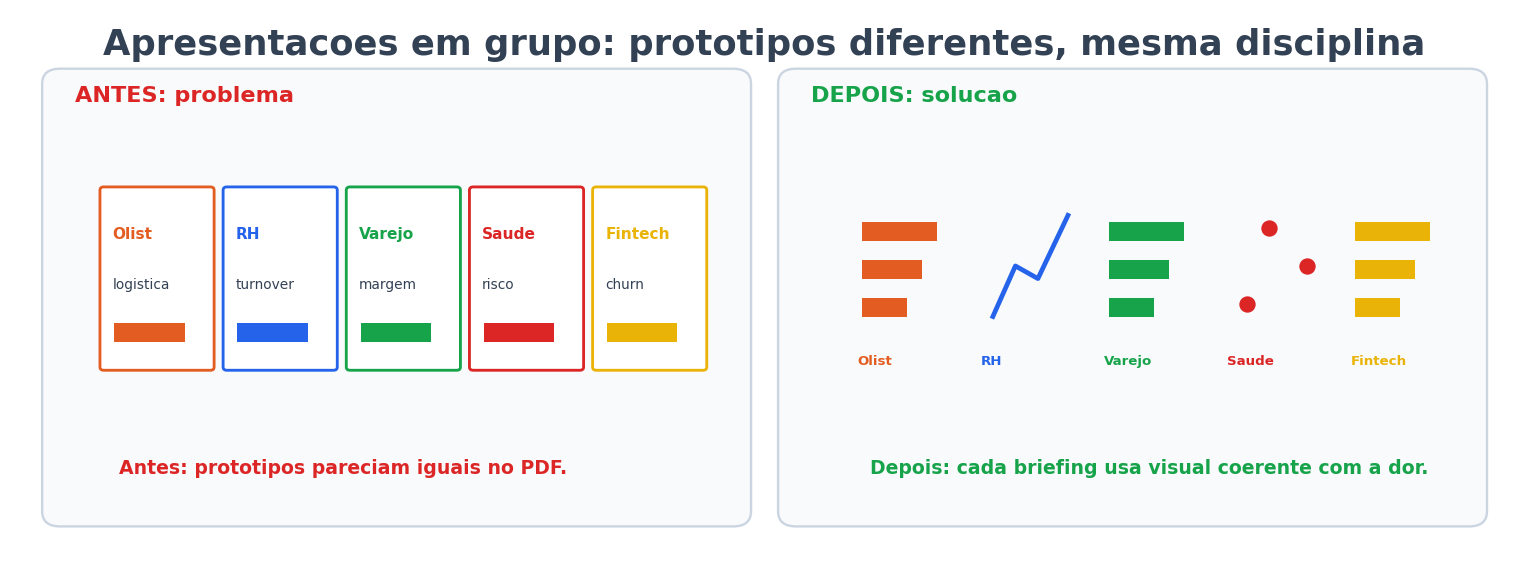
\includegraphics[width=0.62\textwidth]{semana_especial/outputs/cmp_grupos_preview.png}
\end{center}

Os protótipos HTML continuam separados por grupo (\texttt{grupo\_a.html} a \texttt{grupo\_e.html}), mas a figura acima resume a diferença esperada entre eles: cada briefing deve ter visual próprio, coerente com a dor de negócio, e não uma cópia do mesmo layout com dados trocados.
% -------------------------------------------------------

\subsection{Grupo 1 --- E-commerce (Olist)}

\textbf{Dataset:} Brazilian E-Commerce Public Dataset (Olist)\\
\url{https://www.kaggle.com/datasets/olistbr/brazilian-ecommerce}

\textbf{Dor:} atrasos na entrega derrubam as avaliações dos clientes e aumentam o churn de vendedores parceiros da plataforma.

\textbf{Pergunta 1:} ``Em quais estados e categorias os atrasos são mais críticos e qual o impacto nas avaliações (review\_score)?'' \quad \textbf{Pergunta 2:} ``Como o tempo de entrega em dias se correlaciona com a avaliação do cliente?''

\textbf{Big Idea sugerida:} ``Eletrônicos em SP concentram 34\% dos atrasos e puxam o review médio para 3,2 estrelas --- priorizar logística nessa categoria pode elevar o review para 4,1 e reduzir o churn de vendedores em 15\%.'' \quad \textbf{Call to Action:} redesenhar a rota logística de Eletrônicos em SP até Q3/2026.

\textbf{Transformações necessárias:} (1) Join: \texttt{orders $\bowtie$ order\_items $\bowtie$ products $\bowtie$ customers} (chave: \texttt{order\_id} e \texttt{product\_id}). (2) Campo: \texttt{delivery\_delay = order\_delivered\_customer\_date $-$ order\_estimated\_delivery\_date}. (3) Flag: \texttt{is\_late = IF delivery\_delay > 0 THEN ``Atrasado'' ELSE ``No Prazo'' END}. (4) Traduzir categorias com \texttt{product\_category\_name\_translation.csv}. (5) Filtrar status \texttt{canceled} e \texttt{unavailable}.

\textbf{Sheets:} (1) Big Number (\% atrasados por estado/categoria). (2) Mapa coroplético: estado $\times$ \% atraso. (3) Barras horizontais: Top 10 categorias $\times$ \% atraso, líder em laranja. (4) Scatter: dias de atraso $\times$ review\_score + linha de tendência. (5) Linha temporal de atrasos por mês. \textbf{Protótipo HTML:} \texttt{semana\_especial/grupo\_a.html}.

\subsection{Grupo 2 --- People Analytics (IBM HR)}

\textbf{Dataset:} IBM HR Analytics Employee Attrition\\
\url{https://www.kaggle.com/datasets/pavansubhasht/ibm-hr-analytics-attrition-dataset}

\textbf{Dor:} turnover de 28\% em TI custa R\$450k/ano em recrutamento e perda de conhecimento institucional.

\textbf{Pergunta 1:} ``Qual perfil de funcionário tem maior risco de saída e em qual departamento o problema é mais crítico?'' \quad \textbf{Pergunta 2:} ``Satisfação no trabalho e faixa salarial influenciam o turnover?''

\textbf{Big Idea:} ``Funcionários de TI com menos de 2 anos e sem promoção nos últimos 3 anos têm 3$\times$ mais chance de sair --- mentoria focada nesse perfil pode reduzir o turnover de 28\% para 15\% e economizar R\$270k/ano.''

\textbf{Transformações:} (1) \texttt{Attrition\_Num = IF [Attrition]=``Yes'' THEN 1 ELSE 0 END}. (2) \texttt{Turnover\_Rate = AVG(Attrition\_Num) * 100}. (3) Bins de salário (Baixo $<$ 3k / Médio 3k--7k / Alto $>$ 7k). (4) \texttt{Perfil\_Risco = IF [YearsAtCompany] < 2 AND [YearsSinceLastPromotion] > 2 THEN ``Alto Risco'' END}.

\textbf{Sheets:} Big Number (turnover TI vs meta 15\%); barras por departamento com linha de meta; heatmap satisfação $\times$ faixa salarial $\times$ turnover; scatter anos na empresa $\times$ turnover; bullet chart por departamento. \textbf{Protótipo HTML:} \texttt{semana\_especial/grupo\_b.html}.

\subsection{Grupo 3 --- Varejo (Superstore)}

\textbf{Dataset:} Sample Superstore Dataset\\
\url{https://www.kaggle.com/datasets/vivek468/superstore-dataset-final}

\textbf{Dor:} margens negativas em Tecnologia/Sul drenam R\$120k/trimestre do lucro operacional.

\textbf{Pergunta 1:} ``Quais combinações de subcategoria e região geram prejuízo consistente?'' \quad \textbf{Pergunta 2:} ``Existe correlação entre o desconto aplicado e a margem negativa?''

\textbf{Big Idea:} ``Descontos acima de 20\% em Máquinas e Copiadoras na Região Sul concentram 73\% do prejuízo --- capear o desconto em 12\% pode reverter a margem de $-$4,2\% para $+$5,8\%, gerando R\$85k adicionais por trimestre.''

\textbf{Transformações:} (1) \texttt{Margem\_Pct = SUM([Profit]) / SUM([Sales]) * 100}. (2) Bins de desconto (Sem / 0--10\% / 10--20\% / Acima 20\%). (3) \texttt{Prejuizo = IF [Profit] < 0 THEN ``Prejuízo'' ELSE ``Lucro'' END}.

\textbf{Sheets:} Big Number (margem Tech/Sul vs parâmetro de meta 8\%); mapa de calor subcategoria $\times$ região; scatter desconto $\times$ lucro com linhas de referência (0 no eixo Y; 20\% no eixo X); barras agrupadas por região; linha trimestral de margem. \textbf{Protótipo HTML:} \texttt{semana\_especial/grupo\_c.html}.

\subsection{Grupo 4 --- Saúde Pública (Heart Disease)}

\textbf{Dataset:} Heart Disease UCI Dataset\\
\url{https://www.kaggle.com/datasets/johnsmith88/heart-disease-dataset}

\textbf{Dor:} doenças cardíacas = 38\% das internações municipais (custo médio R\$12k/internação).

\textbf{Pergunta 1:} ``Quais fatores de risco têm maior correlação com diagnóstico de doença cardíaca?'' \quad \textbf{Pergunta 2:} ``Qual faixa etária e perfil clínico priorizar em campanhas preventivas?''

\textbf{Big Idea:} ``Colesterol $>$ 240 + pressão arterial $>$ 140 + idade $>$ 55 anos identificam 73\% dos casos de alto risco com apenas 3 variáveis --- triagem preventiva focada nesse perfil pode reduzir internações em 25\% e gerar R\$2,1M de economia anual.''

\textbf{Transformações:} (1) \texttt{Diagnostico = IF [target]=1 THEN ``Doença'' ELSE ``Sem Doença'' END}. (2) \texttt{Sexo = IF [sex]=1 THEN ``Masculino'' ELSE ``Feminino'' END}. (3) Bins de faixa etária ($<$45 / 45--54 / 55--64 / 65+). (4) \texttt{Perfil\_Risco = IF [chol]>240 AND [trestbps]>140 AND [age]>55 THEN ``Alto Risco'' END}. (5) \texttt{Taxa\_Doenca = AVG([target]) * 100}.

\textbf{Sheets:} Big Number (taxa doença em homens $>$ 55); barras de correlação por fator; heatmap faixa etária $\times$ perfil $\times$ taxa; scatter colesterol $\times$ pressão (cor = diagnóstico, linhas em 240 e 140); boxplot de idade por grupo. \textbf{Protótipo HTML:} \texttt{semana\_especial/grupo\_d.html}.

\subsection{Grupo 5 --- Fintech (Credit Card Churn)}

\textbf{Dataset:} Credit Card Customers Dataset\\
\url{https://www.kaggle.com/datasets/sakshigoyal7/credit-card-customers}

\textbf{Dor:} churn de cartão Premium custa R\$2,1M/ano em receita perdida de juros e anuidade.

\textbf{Pergunta 1:} ``Qual perfil de cliente Premium tem maior propensão ao cancelamento?'' \quad \textbf{Pergunta 2:} ``Frequência de uso e limite de crédito influenciam significativamente o churn?''

\textbf{Big Idea:} ``Clientes Premium com limite $<$ R\$10k e menos de 20 transações/ano têm 4$\times$ mais chance de cancelamento --- engajamento proativo focado nesse perfil pode preservar R\$1,2M em receita anual.''

\textbf{Transformações:} (1) \texttt{Churned = IF [Attrition\_Flag]=``Attrited Customer'' THEN 1 ELSE 0 END}. (2) \texttt{Churn\_Rate = AVG(Churned) * 100}. (3) Bins de limite ($<$ R\$10k / R\$10k--30k / $>$ R\$30k). (4) Bins de uso (Baixa $<$ 20 trans / Média 20--50 / Alta $>$ 50). (5) \texttt{Perfil\_Risco = IF [Total\_Trans\_Ct] < 20 AND [Credit\_Limit] < 10000 THEN ``Alto Risco'' END}.

\textbf{Sheets:} Big Number (churn Premium com limite $<$ R\$10k vs benchmark 8\%); barras faixa de limite $\times$ churn; scatter frequência $\times$ valor médio (cor = churn, linha em 20 transações); linha temporal de churn por segmento; heatmap frequência $\times$ limite $\times$ taxa de churn. \textbf{Protótipo HTML:} \texttt{semana\_especial/grupo\_e.html}.

% -------------------------------------------------------
\section{Rubrica de Avaliação --- Apresentação em Grupo}
% -------------------------------------------------------

\begin{tabular}{|p{4.5cm}|r|p{7.5cm}|}
\hline
\textbf{Critério} & \textbf{Peso} & \textbf{Descrição} \\
\hline
Big Idea + Call to Action & 15\% & Explicitada no pitch: ponto de vista + tensão + stake \\
Estrutura do dashboard   & 20\% & Pergunta $\to$ Big Number + Insight IA $\to$ Gráficos $\to$ Tabela \\
Qualidade dos visuais    & 20\% & Títulos-mensagem; cor com propósito; sem chartjunk \\
Insight IA               & 15\% & Acionável; não genérico; ao lado do Big Number \\
Tableau funcional        & 15\% & $\geq$ 1 filtro ou parâmetro funcionando \\
Pitch de 3 minutos       & 15\% & SCR completo; dentro do tempo; call to action explícito \\
\hline
\textbf{Total}           & \textbf{100\%} & \\
\hline
\end{tabular}

% \includegraphics paths são relativos ao diretório de main.tex (aula/)
% =============================================================================

\chapter{Semana Especial (04/05 + 18/05/2026)\\[4pt]Revisão Unidade~II e Dashboard em Grupo}

Este impresso cobre as duas últimas aulas antes das provas. No dia \textbf{04/05} fazemos a revisão de toda a Unidade~II. No dia \textbf{18/05} cada grupo apresenta o dashboard no Tableau --- como está descrito na Parte~III deste documento, que você já recebe hoje para ter duas semanas de preparo. As provas começam na semana de \textbf{25/05}.

% ============================================================
\section*{\Large PARTE I --- REVISÃO DA UNIDADE II (04/05/2026)}
% ============================================================

% -------------------------------------------------------
\section{AED vs.\ Análise Explanatória}
% -------------------------------------------------------

Na Unidade~I vocês exploraram dados para \emph{entender}: histogramas, boxplots, correlações, dados ausentes. A pergunta que guiava cada análise era ``o que os dados me dizem?'' A Unidade~II começa com uma mudança radical de perspectiva. A pergunta agora é outra: \textit{``como eu conto essa história para que alguém tome uma decisão?''}

Quando você sai do papel de analista e entra no papel de comunicador, você faz análise \textbf{explanatória}. A audiência mudou: não é mais você mesmo --- é o CEO, o gerente, o comitê de crédito. Essas pessoas não têm tempo para ver os 200 gráficos que você gerou. Elas precisam de uma mensagem clara suportada pelas evidências certas.

O erro mais comum de analistas iniciantes é mostrar todo o processo exploratório para uma audiência executiva. O resultado: confusão, perda de tempo, e a descoberta mais importante se perde no meio de 30 gráficos. Na análise explanatória, você já sabe a história que vai contar e escolhe \emph{apenas} os gráficos que a sustentam.

\begin{BoardBox}[title=AED vs.\ Explanatória]
\begin{tabular}{@{}lp{4.2cm}p{5.2cm}@{}}
\toprule
 & \textbf{Exploratória (AED)} & \textbf{Explanatória} \\
\midrule
Audiência & O analista & CEO, gerente, investidor \\
Objetivo  & Entender o dado & Provocar uma decisão \\
Linguagem & ``O dado mostra X'' & ``O que este dado muda no que você faz?'' \\
Visuais   & Centenas (maioria descartada) & Só os que servem à mensagem \\
\bottomrule
\end{tabular}
\end{BoardBox}

Toda vez que você estiver construindo uma apresentação, faça esta pergunta para cada gráfico: ``este visual serve à mensagem ou serve à minha curiosidade?'' Se for a segunda opção, ele vai para o apêndice.

\begin{center}
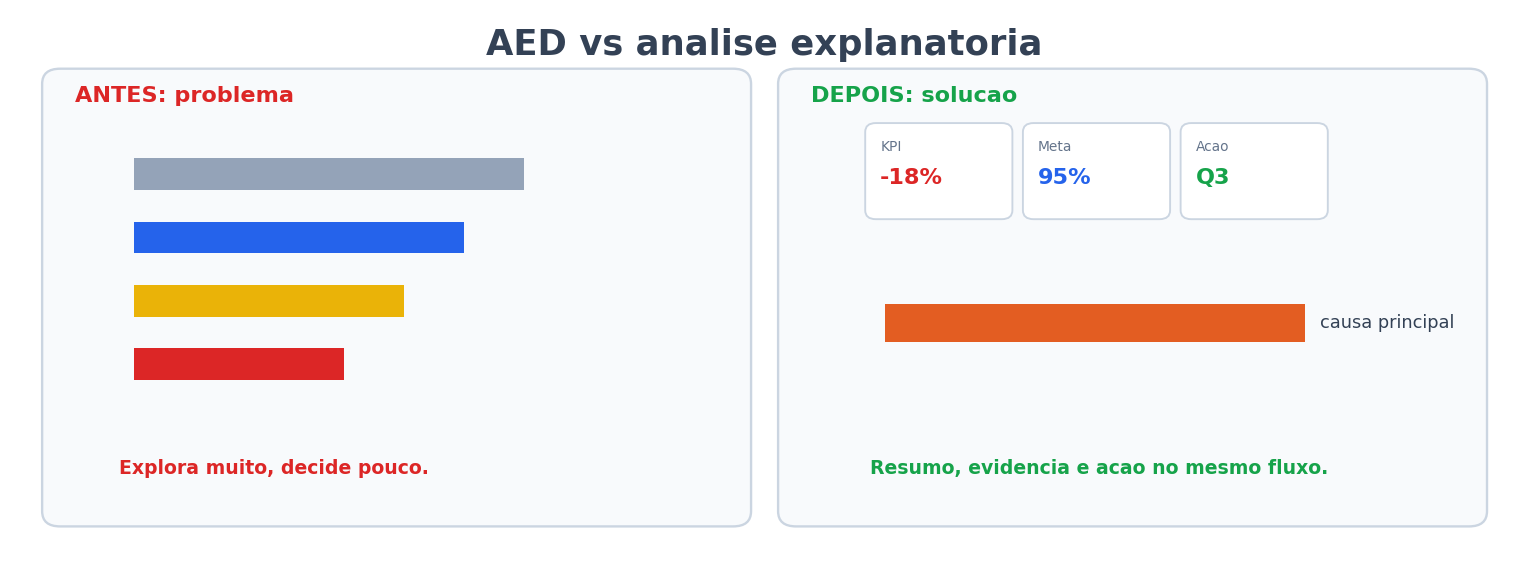
\includegraphics[width=0.58\textwidth]{semana_especial/outputs/cmp_cap2_aed_explanatoria.png}
\end{center}

\textbf{Exemplo prático:} você está analisando dados de alunos em uma instituição de ensino. Na perspectiva exploratória, você gera: correlação entre horas estudadas e nota (0,58), distribuição de notas por sexo, boxplot por disciplina, análise de outliers, falta versus nota. Tudo isso é válido para \emph{você entender} o dado. Mas quando você entra em uma reunião com o diretor e tem 10 minutos, você escolhe apenas \textbf{uma} visualização: alunos com envolvimento familiar baixo + menos de 15 horas de estudo têm nota 9 pontos abaixo da média. Isso é explanatória. A pergunta que o diretor responde depois de ver esse gráfico não é ``que curioso'' --- é ``o que fazemos para resgatar esses alunos?''

% -------------------------------------------------------
\section{Big Idea Framework}
% -------------------------------------------------------

A Big Idea é \textbf{uma única frase} que captura a essência da sua mensagem. Nancy Duarte, em \textit{Datastory} (2019), define que toda boa apresentação de dados deve ter uma Big Idea que a pessoa leva para casa mesmo sem ter visto nenhum gráfico. Ela é o título do seu argumento --- não do seu relatório.

Ela exige três componentes: (1) um \textbf{ponto de vista} --- uma afirmação, não uma observação neutra; (2) a \textbf{tensão} --- o que está em jogo se nada for feito; (3) o \textbf{stake} --- por que a audiência deveria se importar. A fórmula prática é: [recomendação de ação] + [dado concreto que justifica] + [impacto se nada mudar].

\begin{BoardBox}[title=Big Idea --- 3 Componentes e Fórmula]
\begin{enumerate}
  \item \textbf{Ponto de vista:} afirmação, não observação.
  ``O dado mostra X'' \textrightarrow{} não é Big Idea.
  ``Devemos fazer Y porque X'' \textrightarrow{} é Big Idea.
  \item \textbf{Tensão:} o que está em jogo? Risco de não agir?
  \item \textbf{Stake:} por que a audiência deveria se importar?
\end{enumerate}
\smallskip
\textbf{Fórmula:} [ação recomendada] + [dado que justifica] + [impacto financeiro/operacional]
\end{BoardBox}

Veja a diferença: ``A taxa de cancelamento subiu 12\%'' é uma observação --- não orienta nenhuma decisão. ``Se não corrigirmos o onboarding até setembro, perderemos R\$1,2M em receita recorrente nos próximos 12 meses'' tem ponto de vista (corrigir o onboarding), tensão (se não fizermos nada) e stake (R\$1,2M). Essa frase é Big Idea.

O \textbf{teste}: leia para alguém que não viu os dados. Se a resposta for ``interessante'' sem que a pessoa saiba o que fazer --- a Big Idea não está pronta. Ela deve provocar a pergunta ``e como a gente faz isso?''

\begin{center}
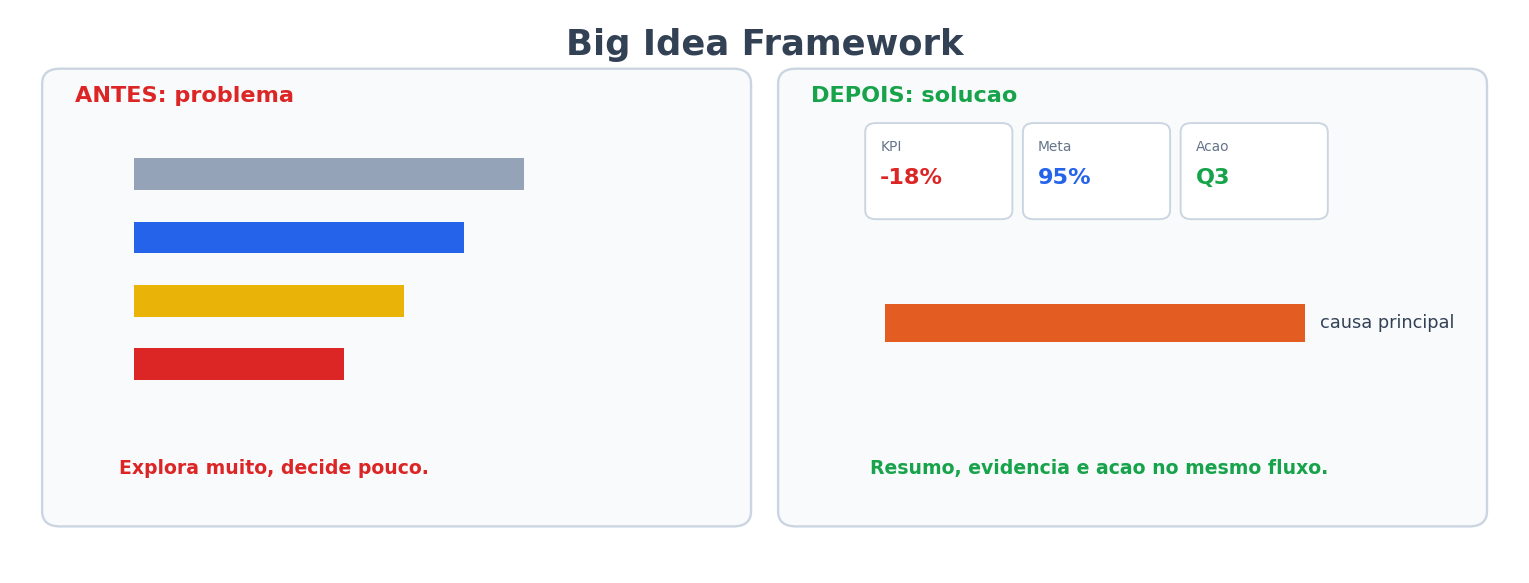
\includegraphics[width=0.58\textwidth]{semana_especial/outputs/cmp_cap2_big_idea.png}
\end{center}

Toda Big Idea está ligada a uma \textbf{pergunta de decisão}: a questão que a audiência precisa responder ao final. Exemplos: ``Devemos expandir para o canal digital ou reforçar o físico?''; ``Qual produto descontinuamos no Q3?''. O analista não precisa ter a resposta --- mas deve apresentar os dados que tornam a resposta possível.

\textbf{Mais exemplos de Big Ideas em diferentes domínios:}
\begin{itemize}
  \item \textit{E-commerce:} ``Frete grátis acima de R\$100 aumenta o ticket médio em 34\%, mas reduz a margem em apenas 8\% --- implementar já seria rentável no Q3.''
  \item \textit{RH:} ``Desenvolvedores sem promoção em 3 anos têm 5$\times$ mais chance de sair; implementar plano de carreira acelerado para 23 talentos preservaria R\$480k em custos de reposição anual.''
  \item \textit{Saúde:} ``Pacientes que recebem chamada de lembrete 24h antes da consulta aumentam a taxa de comparecimento em 41\%; reduz custos operacionais em R\$120k/ano.''
\end{itemize}

\textbf{Teste na prática:} leia sua Big Idea para um colega que não mexe com seus dados. Se ele disser ``muito interessante'', ela ainda não está pronta. Se ele disser ``e quando a gente começa?'', pronto --- você tem uma Big Idea de verdade.

% -------------------------------------------------------
\section{Storyboard e Estrutura Narrativa}
% -------------------------------------------------------

Antes de abrir o Tableau e construir qualquer gráfico, você desenha o \textbf{storyboard} --- um rascunho em papel com os títulos das telas e o tipo de visual em cada uma. Ele força você a pensar na narrativa \emph{antes} de pensar nas ferramentas. Quem abre o Tableau sem storyboard constrói gráficos bonitos sem história.

Nancy Duarte propõe uma estrutura de 4 atos adaptada de narrativas clássicas. O truque é que toda boa apresentação de dados segue exatamente essa ordem: você mostra o estado atual, revela a tensão, apresenta a proposta e termina com um pedido concreto.

\begin{BoardBox}[title=Estrutura Narrativa --- 4 Atos]
\begin{enumerate}
  \item \textbf{Contexto --- O que é:} estado atual; KPIs reais; o ponto de partida.
  \item \textbf{Conflito --- O que poderia ser:} a tensão; o dado que revela o problema.
  \item \textbf{Resolução --- O que proponho:} proposta baseada em evidências.
  \item \textbf{Call to Action:} decisão pedida + responsável + prazo.
\end{enumerate}
\smallskip
\textbf{Em telas:} KPIs atuais \textrightarrow{} problema \textrightarrow{} análise/evidências \textrightarrow{} recomendação
\end{BoardBox}

Cada tela do storyboard deve ter: (1) título que é mensagem --- não ``Gráfico de Barras'', mas sim ``Canal físico custa 4$\times$ mais por venda''; (2) tipo de visual proposto; (3) esboço manual do dado; (4) transição lógica para a próxima tela, como ``por isso, na próxima tela, veja\ldots''

\begin{center}
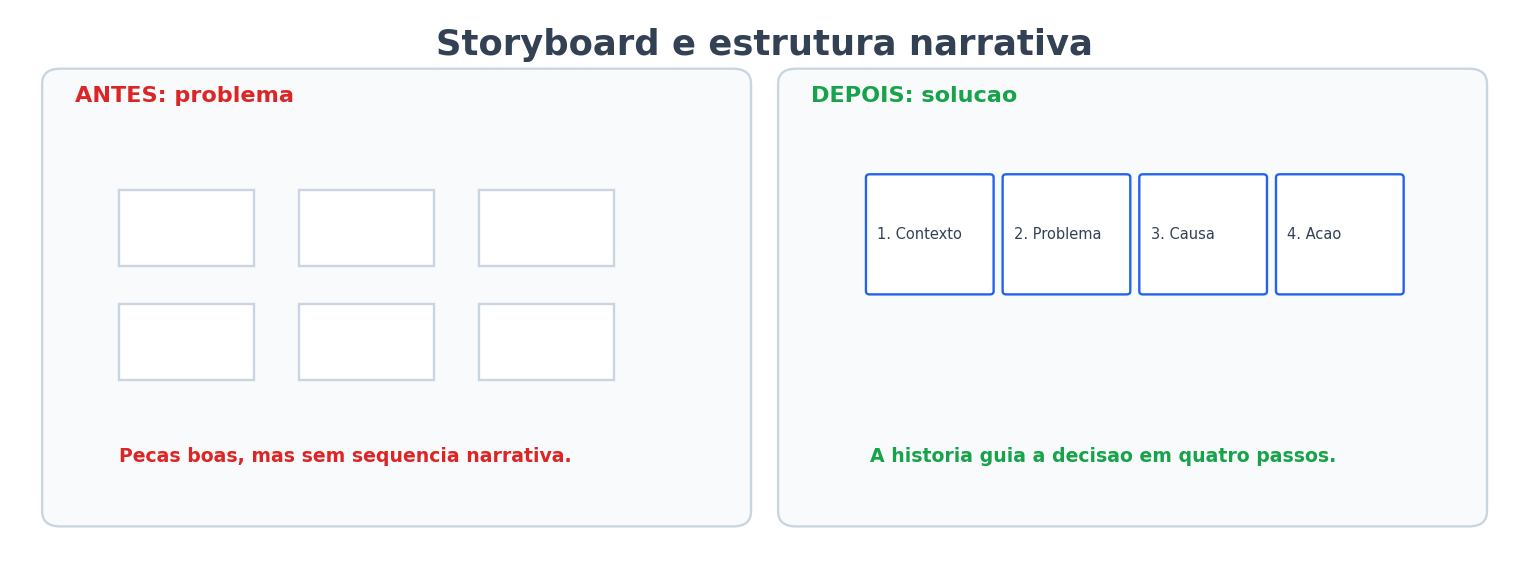
\includegraphics[width=0.58\textwidth]{semana_especial/outputs/cmp_cap2_storyboard.png}
\end{center}

\textbf{Exemplo de storyboard em 4 telas de uma apresentação executiva:}
\begin{enumerate}
  \item \textbf{Tela 1 --- Contexto:} ``Vendas em regiões Sul e Centro-Oeste crescem 15\% acima da média nacional.'' (Big Number destacado + KPI) Transição: ``mas quando olhamos a margem, a história muda radicalmente.''
  \item \textbf{Tela 2 --- Conflito:} ``Essas mesmas regiões têm margem negativa em Tecnologia.'' (Scatter: Desconto vs Margem, cor vermelho no quadrante negativo) Transição: ``achamos 3 subcategorias que concentram 73\% do prejuízo.''
  \item \textbf{Tela 3 --- Análise:} ``Máquinas em SP têm desconto médio de 26\%; Copiadoras em Sul, 23\%; comparando com Nordeste (14\%), o culpado é a política de desconto regional.'' (Tabela + box destacando as 3 categorias críticas) Transição: ``por isso recomendamos\ldots''
  \item \textbf{Tela 4 --- Recomendação:} ``Capar desconto máximo em 12\% em Tecnologia/Sul até 01/junho recupera R\$85k de margem trimestral e move o resultado de -4,2\% para +5,8\%.'' (Simulação com 3 cenários: otimista, realista, pessimista) Próximo passo: ``Gerência Comercial, confirmar a implementação até 15/maio?''
\end{enumerate}

O storyboard em papel \textbf{antes de você abrir o Tableau} economiza semanas de trabalho. Você já sabe qual série temporal é importante, qual drill-down você precisa, quantas telas usará. Quem pula essa etapa muitas vezes constrói um dashboard tecnicamente correto mas narrativamente confuso.

% -------------------------------------------------------
\section{Design de Informação: Pré-atenção e Atributos Visuais}
% -------------------------------------------------------

Antes de você ler deliberadamente qualquer coisa num gráfico, seu cérebro já detectou alguns elementos em menos de 250 milissegundos, sem esforço consciente. Esses são os \textbf{atributos pré-atencionais}. Se você os usa para destacar o que importa, o leitor chega à mensagem antes de ler o título. Se os usa aleatoriamente, o leitor fica desorientado.

A regra de ouro é usar no máximo \textbf{dois atributos pré-atencionais} por visual. Acima disso, a hierarquia colapsa e o olho não sabe onde pousar.

\begin{BoardBox}[title=Atributos Pré-atencionais]
\begin{tabular}{@{}llp{5.2cm}@{}}
\toprule
\textbf{Atributo} & \textbf{Função} & \textbf{Regra de uso} \\
\midrule
Cor        & Destaca, agrupa       & 1 cor de destaque; resto em cinza neutro \\
Tamanho    & Indica magnitude      & Maior = mais importante; consistência obrigatória \\
Posição    & Organiza hierarquia   & Mais importante: canto superior esquerdo \\
Intensidade & Contraste claro/escuro & Mais escuro = mais importante \\
Enclosure  & Agrupa elementos      & Caixa ao redor de dados relacionados \\
\bottomrule
\end{tabular}
\end{BoardBox}

A \textbf{cor} merece atenção especial. Há a cor semântica (vermelho = alerta, verde = ok, amarelo = atenção) e a cor de destaque (uma cor viva para o elemento que carrega a mensagem; todo o resto em cinza). Use cor semântica onde já existe convenção estabelecida. Nunca inverta vermelho e verde sem motivo forte. E lembre: 8\% dos homens têm daltonismo vermelho-verde --- evite que essa combinação seja o único diferenciador.

\begin{center}
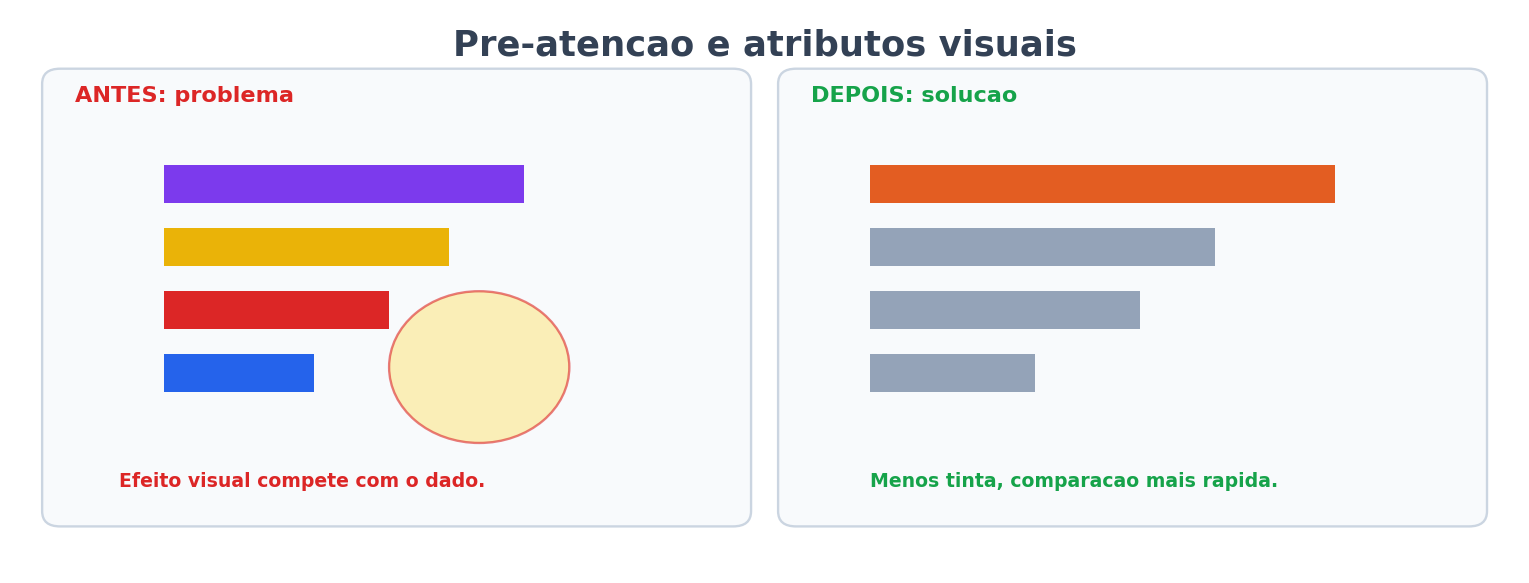
\includegraphics[width=0.58\textwidth]{semana_especial/outputs/cmp_cap2_preatencao.png}
\end{center}

\textbf{Regra de ouro revisitada:} você consegue usar até 2 atributos pré-atencionais em harmonia. Exemplo: na ábaco visual mostrando performance por time, use \textbf{COR} para semântica (verde = meta atingida, vermelho = abaixo) e \textbf{TAMANHO} para magnitude (bolinha grande = time grande, bolinha pequena = time pequeno). Juntos, os dois atributos permitem decodificação instantânea. Se você adicionar um terceiro --- posição espacial não óbvia, ou intensidade de padrão --- o cérebro fica sobrecarregado e falha no teste do relance. Na prática, quando você entra na dúvida de ``será que está confuso?'', sempre está. Remova o terceiro atributo.

% -------------------------------------------------------
\section{Teste do Relance e Título-Mensagem}
% -------------------------------------------------------

O Teste do Relance é simples: mostre o gráfico por 3 segundos, cubra e pergunte à audiência o que viram e qual a mensagem principal. Se não conseguirem responder em 3 segundos, o visual falhou. Não o leitor --- o design.

\begin{BoardBox}[title=Teste do Relance --- Diagnóstico de Falha]
Causas mais comuns de falha:
\begin{itemize}
  \item Título rótulo em vez de título mensagem
  \item Excesso de elementos --- o olho não sabe onde pousar
  \item Cores sem propósito --- todas as barras em cores diferentes
  \item Legenda separada --- o leitor desvia o olhar para decodificar
\end{itemize}
\smallskip
\textbf{Fórmula do título mensagem:} [Sujeito] + [verbo de tendência] + [magnitude]\\
Ex.: ``Churn \textbf{caiu} 34\% após o programa de fidelidade''
\end{BoardBox}

A diferença entre título rótulo e título mensagem é a diferença entre ``Vendas por Região'' e ``Região Sul concentra 58\% das vendas''. O primeiro descreve o que o eixo mostra. O segundo já entrega a informação. Para o executivo com 5 minutos por dia, o título mensagem é o gráfico mais importante --- porque ele consegue ler apenas os títulos e já sabe o que decidir.

\begin{center}
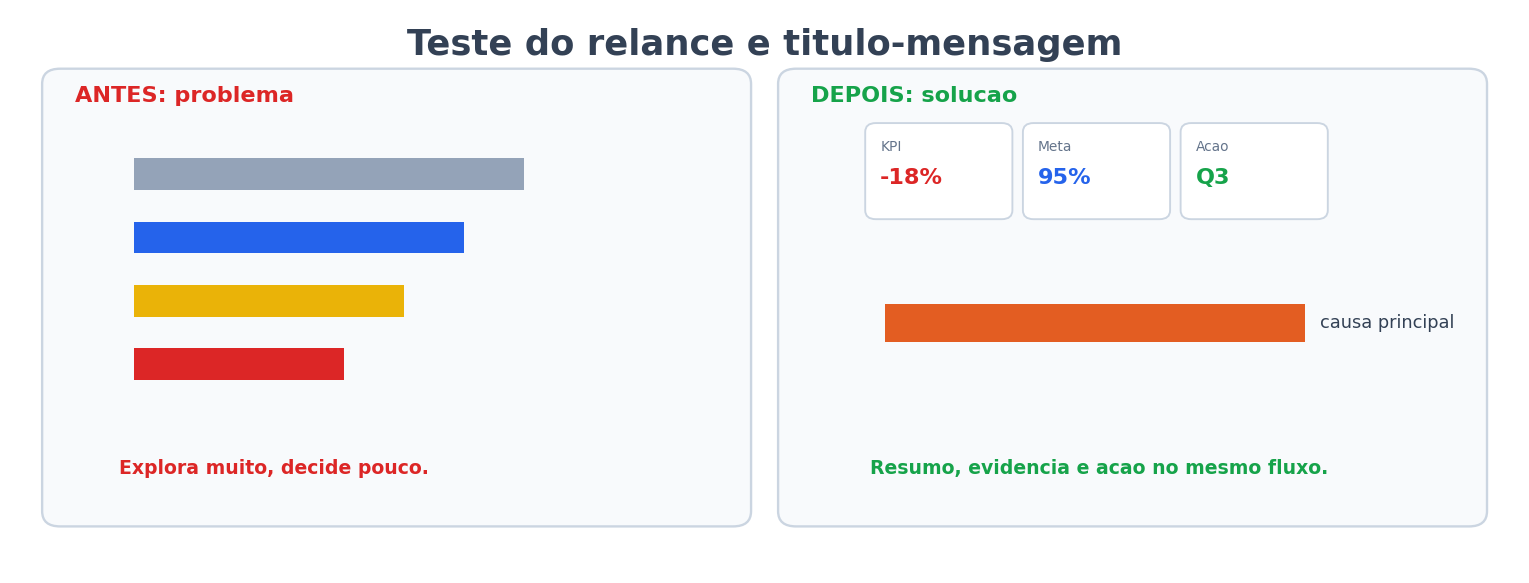
\includegraphics[width=0.58\textwidth]{semana_especial/outputs/cmp_cap2_relance.png}
\end{center}

\textbf{Checklist para passar no Teste do Relance:} (1) título é mensagem, não rótulo? (2) cores comunicam semântica ou prioridade, não decoração? (3) gráfico tem exatamente 1 ou 2 atributos pré-atencionais, não mais? (4) sem ambiguidade: alguém que não viu o dado sabe imediatamente qual a mensagem?

Quando você apresenta um dashboard para alguém pela primeira vez, teste na prática: mostre por 3 segundos, tape a tela e pergunte ``qual a mensagem principal deste gráfico?'' Se a resposta não estiver clara, você ainda tem trabalho. Se estiver absolutamente cristalina --- pronto, passou.

% -------------------------------------------------------
\section{Data-Ink Ratio e Chartjunk}
% -------------------------------------------------------

Edward Tufte (1983) propõe o conceito de \textbf{data-ink ratio}: a proporção da tinta do gráfico que realmente representa dados sobre a tinta total. Maximize esse ratio. Tudo que ocupa tinta sem carregar informação é candidato à remoção.

\begin{BoardBox}[title=Data-Ink Ratio e Chartjunk]
\[
  \text{Data-ink ratio} = \frac{\text{tinta que representa dados}}{\text{tinta total do gráfico}}
\]
\textbf{Chartjunk --- remova:} grades pesadas $\cdot$ barras 3D $\cdot$ sombras $\cdot$ gradientes decorativos $\cdot$ legendas redundantes $\cdot$ ícones temáticos $\cdot$ mais de 3 casas decimais\\[4pt]
\textbf{Princípio:} ``Se eu remover isso, o gráfico fica menos claro?'' Se não --- remova.
\end{BoardBox}

O gráfico de pizza com 8 fatias em 8 cores é o exemplo clássico de chartjunk. O olho humano não compara ângulos com precisão; ele compara comprimentos. Substitua pizza por barras horizontais ordenadas, com 1 cor de destaque para a categoria que carrega a mensagem e rótulos diretos nas barras --- elimine a legenda.

\begin{center}
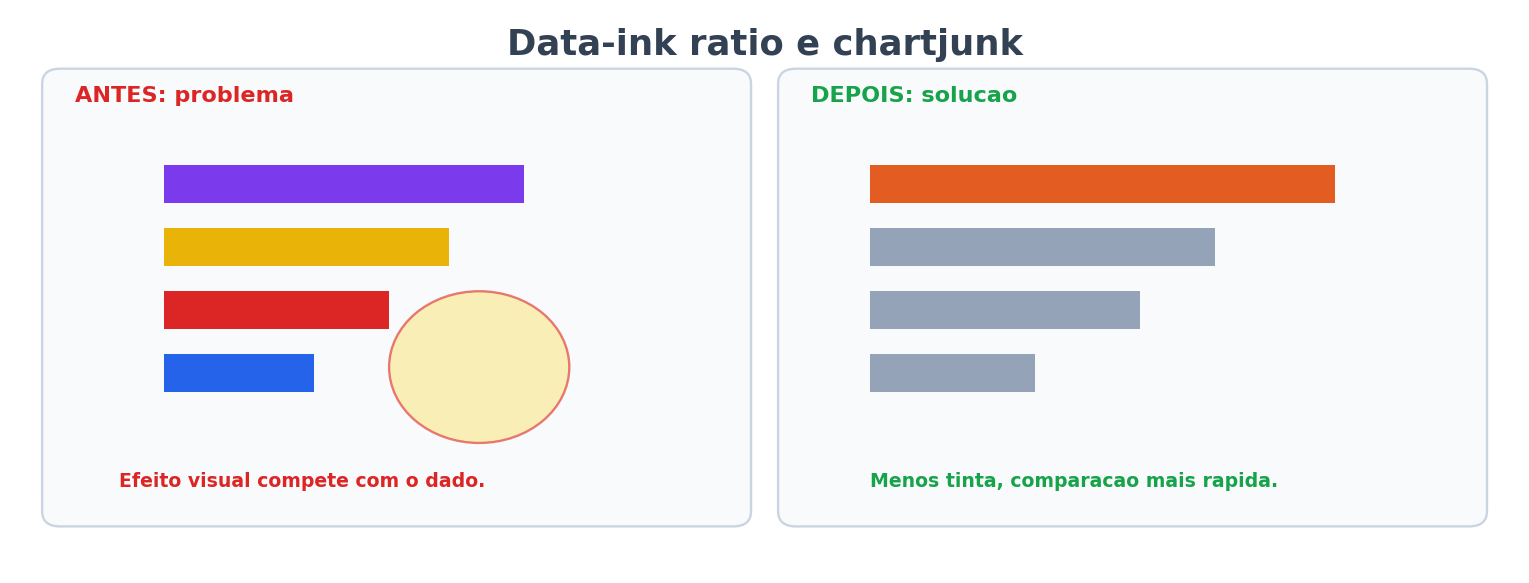
\includegraphics[width=0.58\textwidth]{semana_especial/outputs/cmp_cap2_chartjunk.png}
\end{center}

\textbf{Exemplo de eliminação de chartjunk em 3 passos:} Você tem um gráfico de barras com: (1) grid pesado horizontal e vertical (remove); (2) barras com borda preta (remove); (3) sombra abaixo das barras (remove); (4) legenda no lado dizendo ``Série 1'' (remove --- coloque o rótulo direto na barra); (5) números com 3 casas decimais (reduz para 1 ou 2). Resultado final: data-ink ratio sobe de 50\% para 85\%, o gráfico fica 70\% menor em tamanho visual, e a mensagem fica mais clara.

Em Tableau, a regra é simples: remova toda grid, remova border das marcas, use espaçamento generoso, e ative os rótulos diretos. O resultado é um visual que cabe em uma tela de executivo sem parecer ``deserto''.

% -------------------------------------------------------
\section{Tableau: Filtros, Parâmetros e Ações}
% -------------------------------------------------------

Dois recursos fundamentais de interatividade no Tableau que os alunos frequentemente confundem. A diferença é direta: \textbf{filtros} incluem ou excluem linhas do dataset; \textbf{parâmetros} mudam o cálculo sem filtrar nenhuma linha. Um filtro por estado exibe só os dados de PE --- os dados de SP desaparecem da view. Um parâmetro de métrica permite que o usuário escolha entre Receita ou Margem --- nenhum dado é excluído, apenas o campo calculado muda.

\begin{BoardBox}[title=Filtros vs.\ Parâmetros]
\begin{tabular}{@{}lp{4.5cm}p{5.2cm}@{}}
\toprule
 & \textbf{Filtro} & \textbf{Parâmetro} \\
\midrule
Função   & Inclui/exclui linhas      & Muda o cálculo \\
Uso      & Selecionar região, categoria & Alternar métrica, definir meta, Top N \\
Exemplo  & ``Ver só PE''             & ``Exibir Receita ou Margem?'' \\
\bottomrule
\end{tabular}
\smallskip

\textbf{Campo calculado com parâmetro:}\\
\texttt{IF [Vendas] >= [Meta] THEN ``Atingiu'' ELSE ``Abaixo'' END}
\end{BoardBox}

Sobre a \textbf{hierarquia de filtros}: o Tableau executa filtros em ordem fixa. O mais importante para a prova é o \textbf{Context Filter}. Quando você precisa de Top~N dentro de uma região já filtrada, adicione o filtro de região como Context Filter primeiro --- senão o Tableau calcula o Top~N sobre o dataset inteiro, ignorando o filtro de região.

\begin{center}
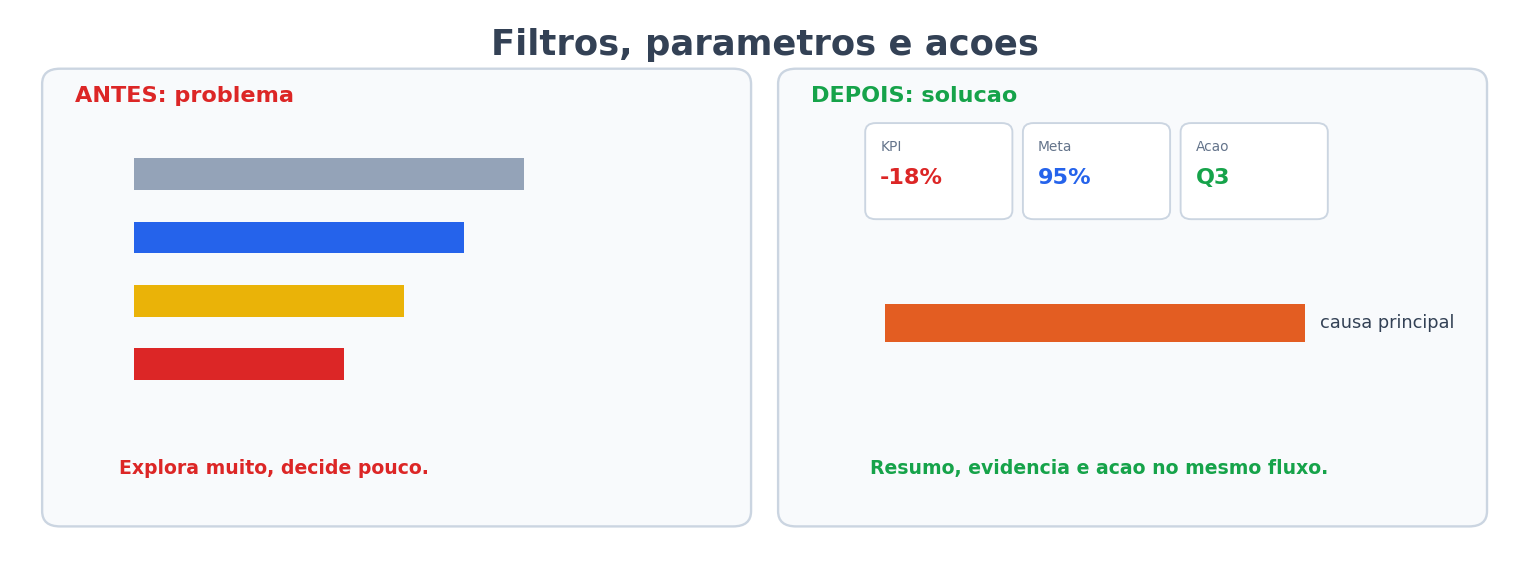
\includegraphics[width=0.58\textwidth]{semana_especial/outputs/cmp_cap2_tableau.png}
\end{center}

\textbf{Pseudocódigo Tableau para parâmetros:} você cria um parâmetro chamado \verb|[Métrica_Selecionada]| com opções ``Receita'', ``Margem'', ``Unidades''. Depois cria um campo calculado:
\begin{quote}\ttfamily
IF [Métrica\_Selecionada] = ``Receita'' THEN [Receita]\\
ELSEIF [Métrica\_Selecionada] = ``Margem'' THEN [Margem]\\
ELSE [Unidades] END
\end{quote}
Quando o usuário muda o parâmetro, o campo calculado avalia instantaneamente e todo o dashboard reflete a mudança. Nenhuma linha é filtrada, apenas o cálculo muda.

\textbf{Context Filter --- quando usar:} você está vendo Top 10 Produtos por Receita em São Paulo. Se você não adicionar ``Estado = SP'' como Context Filter, o Top 10 é calculado sobre TODOS os estados, depois filtrado --- resultado: pode aparecer um produto de outro estado. Com Context Filter, o Top 10 é calculado apenas em SP, garantindo que os 10 maiores de SP apareçam.

\begin{BoardBox}[title=Ações de Dashboard --- 4 Tipos]
\begin{tabular}{@{}lp{4cm}p{4.8cm}@{}}
\toprule
\textbf{Tipo}     & \textbf{O que faz}                  & \textbf{Exemplo} \\
\midrule
Filter action   & Clicar filtra outra view             & Clicar em SP filtra todos os gráficos \\
Highlight       & Destaca sem filtrar                  & Mouse em Região destaca no mapa \\
URL action      & Abre URL com dado selecionado        & Clique abre ficha no ERP \\
Navigate        & Navega entre dashboards              & KPI leva ao painel de drill-down \\
\bottomrule
\end{tabular}
\end{BoardBox}

% -------------------------------------------------------
\section{Dashboards que Forçam Decisão}
% -------------------------------------------------------

Um dashboard pode ser tecnicamente impecável e ainda assim não provocar nenhuma ação. O problema, nesse caso, é de estrutura narrativa. Um dashboard que \textbf{força uma decisão} tem três zonas distintas e em sequência.

\begin{BoardBox}[title=As 3 Zonas do Dashboard Decisório]
\textbf{Zona 1 --- Contexto:} o que está acontecendo agora? KPIs com comparação à meta ou período anterior. Lido em $<$5 segundos. Nenhuma interpretação ainda.

\textbf{Zona 2 --- Diagnóstico:} por que está acontecendo? Drill-down por produto, região, segmento. Permite formular hipóteses --- não confirmar causas.

\textbf{Zona 3 --- Recomendação:} o que fazer? 1--2 recomendações concretas com evidências. Call to Action com \emph{quem}, \emph{o quê} e \emph{até quando}.
\end{BoardBox}

Os \textbf{anti-padrões} mais comuns: (a) tudo sempre verde --- cria conforto falso e impede decisões urgentes; (b) métricas sem definição --- ``Receita'' pode ser bruta, líquida ou MRR, e sem definição explícita cada pessoa lê diferente; (c) 50~KPIs na tela inicial --- granularidade excessiva, o usuário não sabe onde olhar; (d) número isolado sem comparação --- R\$100k de vendas é ótimo ou péssimo em relação ao quê?

\begin{center}
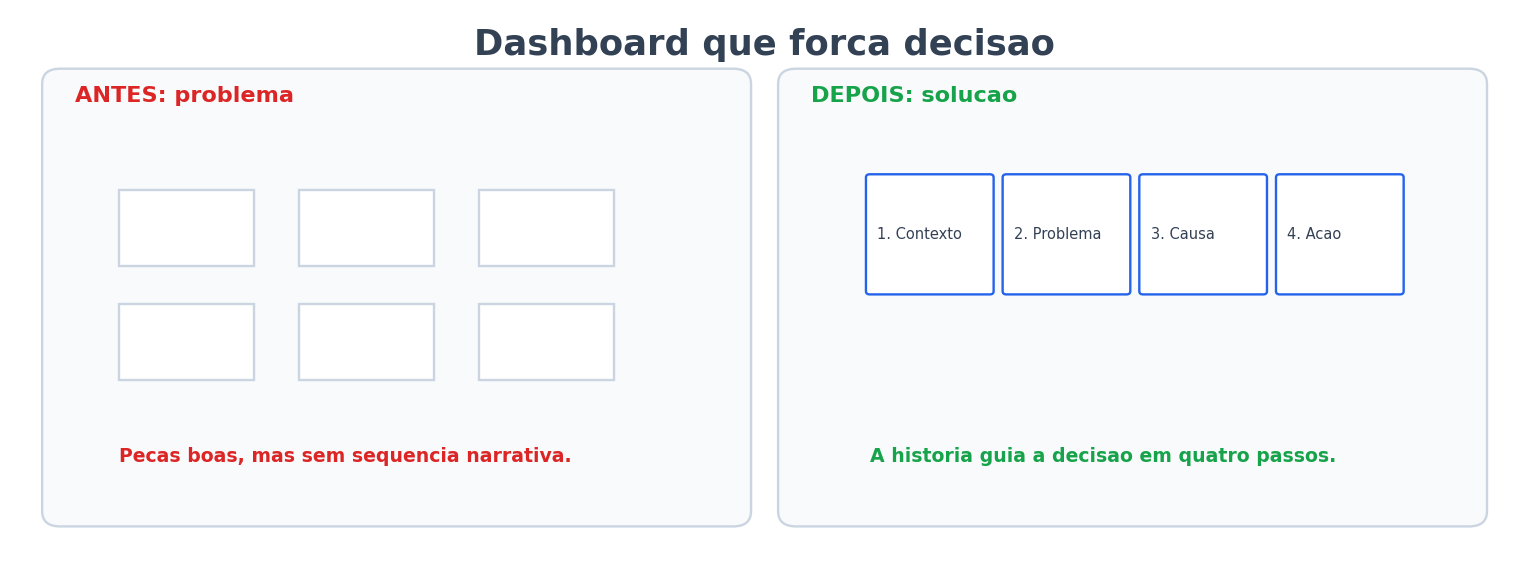
\includegraphics[width=0.58\textwidth]{semana_especial/outputs/cmp_cap2_decisorio.png}
\end{center}

\textbf{Implementação prática das 3 zonas em um dashboard de Vendas:}
\begin{itemize}
  \item \textbf{Zona 1 (Contexto):} 4 KPIs acima da dobra: (1) Receita Mês, Meta, Gap; (2) Margem %; (3) Churn; (4) NPS. Cada KPI mostra ícone de semáforo (verde/amarelo/vermelho). Tempo de leitura: <3 segundos. Nenhuma ação ainda.
  \item \textbf{Zona 2 (Diagnóstico):} 3 gráficos lado a lado: (1) Receita por Região (barras horizontais); (2) Churn vs Desconto (scatter); (3) Série temporal de Margem (linha com meta). Permite que o usuário formule hipóteses (``RJ tem desconto alto demais?'') mas não confirma causas.
  \item \textbf{Zona 3 (Recomendação):} 1 caixa destacada em cor de alerta: ``RJ concentra 65\% da receita mas margem negativa. Reduzir desconto de 26\% para 12\% recupera R\$85k trimestral sem impactar volume (elasticidade = 0,34). Gerência Comercial: implementar até 30/junho.''
\end{itemize}

\textbf{Teste de efetividade:} se seu gerente consegue ler apenas a Zona 3 e já tem uma decisão clara e acionável, sua estrutura funcionou. Se ele precisa voltar para a Zona 2 para entender, significa que a Recomendação não está autossuficiente.

% -------------------------------------------------------
\section{KPIs com Meta, Gap e Tendência}
% -------------------------------------------------------

Um KPI sozinho não decide nada. Para forçar uma decisão, ele precisa de cinco componentes. O número isolado responde ``qual é o valor?'' mas não responde ``isso é bom ou ruim?'' nem ``a situação está melhorando ou piorando?''

\begin{BoardBox}[title=Anatomia de um KPI Decisório]
\begin{enumerate}
  \item \textbf{Valor atual} --- o número real do período
  \item \textbf{Meta (target)} --- o que deveria ser
  \item \textbf{Gap} --- distância em valor absoluto e percentual
  \item \textbf{Tendência} --- seta de alta/baixa ou sparkline
  \item \textbf{Período} --- MTD, YTD, vs ano anterior
\end{enumerate}
\smallskip
\textbf{Bullet chart} (Stephen Few): barra real + barra de meta. Mais informação por cm$^2$ do que qualquer velocímetro ou gauge.
\end{BoardBox}

\begin{center}
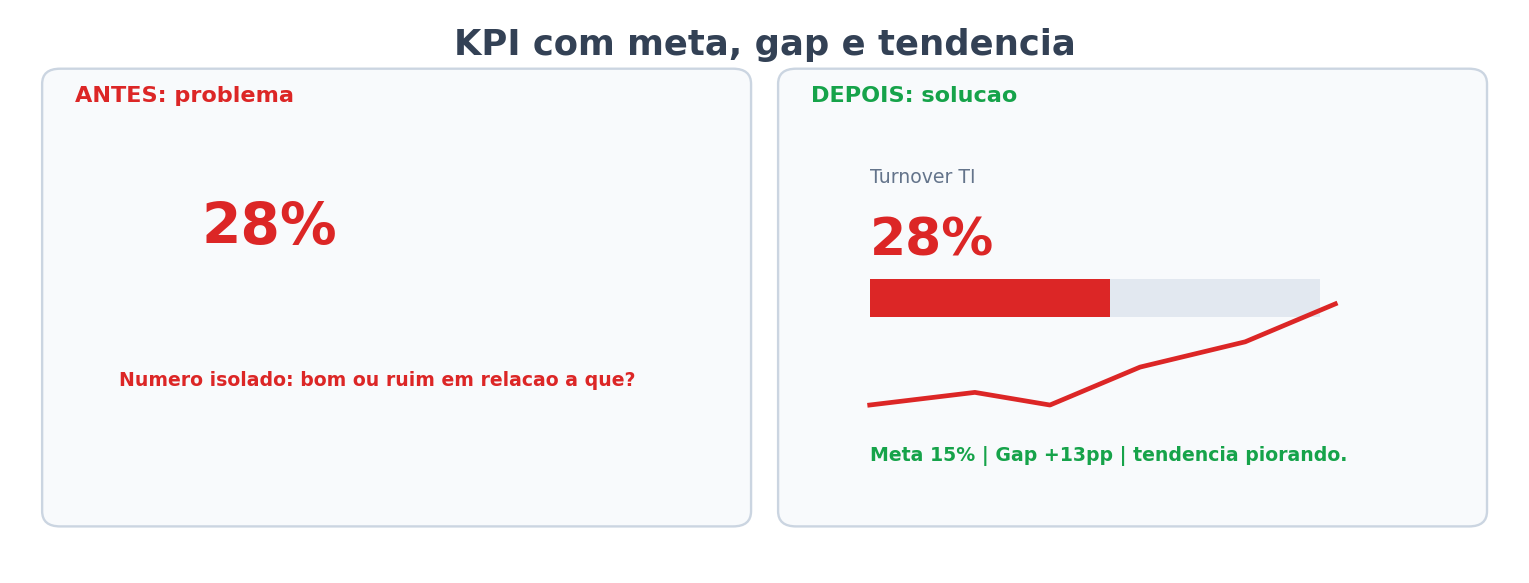
\includegraphics[width=0.58\textwidth]{semana_especial/outputs/cmp_cap2_kpi.png}
\end{center}

\textbf{Exemplos de KPIs bem estruturados em diferentes domínios:}
\begin{itemize}
  \item \textit{E-commerce:} Taxa de Retorno 8\% (Meta: 5\%, Gap: +3pp, Tendência: queda, melhorando, Período: YTD 2026)
  \item \textit{RH:} Turnover TI 28\% (Meta: 15\%, Gap: +13pp, Tendência: alta, piorando, Período: últimos 12 meses)
  \item \textit{Saúde:} Taxa de Readmissão 6,5\% (Meta: 5\%, Gap: +1,5pp, Tendência: alta, piorando, Período: YTD 2026)
\end{itemize}

Quando você tem espaço, a \textbf{bullet chart} (Stephen Few, 2006) é superior ao gauge ou velocímetro porque mostra valor atual, meta, faixa de desempenho bom/médio/ruim, tudo em uma linha horizontal. Se você tiver apenas espaço para um cartão quadrado, use: número grande + meta + gap colorido + sparkline de tendência.

\textbf{Anti-padrão a evitar:} número isolado na tela. Sempre sempre sempre colocar número com: (1) meta ou benchmark; (2) período; (3) tendência. Caso contrário, o número não informa nada --- pode ser bom, ruim, normal. O contexto é o que faz um número virar insight.

% -------------------------------------------------------
\section{Pitch de 3 Minutos}
% -------------------------------------------------------

Três minutos são aproximadamente 450 palavras. Isso é suficiente para convencer alguém --- se e somente se você seguir a estrutura certa. A estrutura SCR (Situação, Complicação, Resolução) tem quatro blocos com tempos definidos.

\begin{BoardBox}[title=Pitch de 3 Minutos --- Estrutura SCR]
\begin{enumerate}
  \item \textbf{Situação (30s):} contexto factual. Comece com o dado impactante, não com introdução genérica.
  \item \textbf{Complicação (45s):} o problema ou oportunidade revelado. Aqui entra a Big Idea.
  \item \textbf{Resolução (60s):} evidência + recomendação com número concreto. Não ``melhorar'' --- sim ``aumentar em 15\%''.
  \item \textbf{Próximo passo (45s):} pedido específico com \textit{verbo + quem + prazo}.
\end{enumerate}
\end{BoardBox}

O erro mais comum: começar com contexto genérico (``vivemos em uma era de dados\ldots'') em vez do dado que mais surpreende. Se você tem 3 minutos e gasta 30 segundos com introdução desnecessária, perdeu 17\% do tempo e a atenção da audiência.

\begin{center}
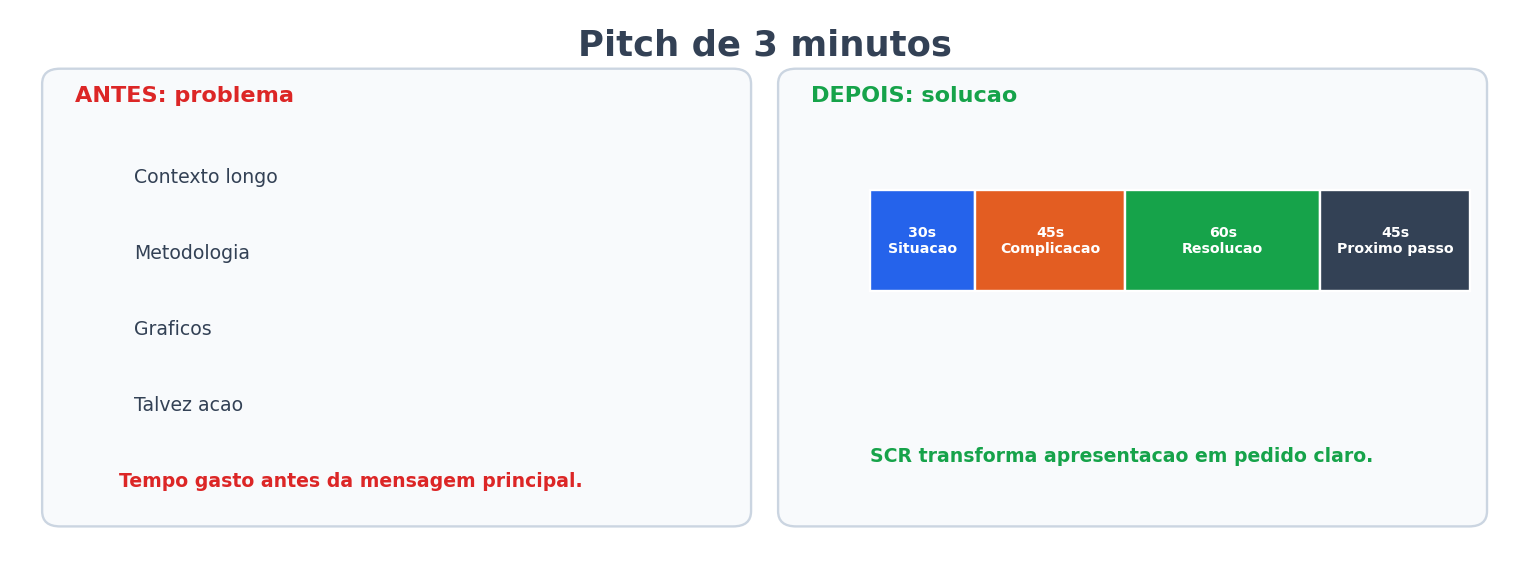
\includegraphics[width=0.58\textwidth]{semana_especial/outputs/cmp_cap2_pitch.png}
\end{center}

\textbf{Exemplo de pitch de 3 minutos em contexto acadêmico:}\\[2pt]
\textbf{Situação (30s):} ``6.607 alunos. 27\% têm nota final menor que 60. Isso significa 1.800 alunos em recuperação, triplicando a carga administrativa e reduzindo a taxa de aprovação final.''\\[2pt]
\textbf{Complicação (45s):} ``Descobrimos que esses alunos compartilham um perfil comum: envolvimento familiar baixo, menos de 15 horas de estudo por semana, e sem ninguém fazendo mentoria. A consequência é uma defasagem de 9 pontos na nota média desse grupo. Se nada mudar, estaremos triplicando esforço e mantendo o mesmo resultado.''\\[2pt]
\textbf{Resolução (60s):} ``Implementamos um programa piloto de mentoria + comunicação familiar com 220 desses alunos em 2025. Resultado: 40\% desse grupo passou a atingir nota acima de 60, aumentando a taxa de aprovação em 8pp e reduzindo custos operacionais de recuperação em R\$45k por ciclo.''\\[2pt]
\textbf{Próximo passo (45s):} ``Recomendo ampliar o programa para todos os alunos em risco (1.800 alunos) no próximo semestre. Implementação começa em julho, com coordenação com coordenação acadêmica. Impacto projetado: +12pp na taxa de aprovação e economia sustentável de R\$120k/ano.''

\textbf{Timing checklist:} você praticou em voz alta? Esse é o teste final. Textos parecem curtos quando lidos mentalmente; no palco, correm 40\% mais rápido do que você pensa. Se você não praticar, vai acabar rápido demais e sobrar tempo, ou vai ficar atropelado tentando terminar em 3 minutos.

% ============================================================
\section*{\Large PARTE II --- QUESTÕES DAS PROVAS --- UNIDADE II}
% ============================================================

As questões abaixo estão no formato exato das provas. \textbf{Prova II Unidade} primeiro (5 questões de 2,0 pts cada). Depois as questões de Unidade~II da \textbf{Prova Final} (Q8, Q9 e Q10 --- 1,0 pt cada). Por fim as questões de Unidade~II da \textbf{Prova II Chamada} (Q8, Q9 e Q10 --- 1,0 pt cada). Os cenários foram levemente adaptados para fins didáticos.

% ============================================================
\subsection*{Prova II Unidade (5 questões $\times$ 2,0 pts)}
% ============================================================

% --- Q1 --- Big Idea
Beatriz é analista de dados em uma rede de 18 farmácias no Recife. Ela foi solicitada a apresentar os resultados de sua análise sobre cancelamentos do programa de fidelidade para a reunião trimestral de diretoria. Após semanas de análise exploratória, Beatriz descobriu que: 72\% dos cancelamentos ocorrem nos primeiros 2 meses; clientes que resgatam pelo menos 1 benefício no primeiro mês têm 80\% de chance de permanecer; o canal de cadastro via WhatsApp tem taxa de retenção 35\% maior que o cadastro em loja; filas no caixa durante o almoço (12h--13h) estão com tempo médio de 8 minutos, gerando reclamações. Beatriz precisa que a diretoria tome uma decisão clara ao final da apresentação.

\begin{SolvedBox}[title=Questão 1 --- Prova II Unidade (2{,}0 pts) --- Big Idea]
Qual alternativa apresenta a \textbf{Big Idea bem formulada} que Beatriz poderia usar?
\begin{enumerate}[label=\Alph*)]
  \item ``Devemos implementar um fluxo de engajamento automático via WhatsApp nos primeiros 2 meses, com nudge para o primeiro resgate, pois isso pode reduzir cancelamentos em até 55\% e aumentar a receita recorrente do programa em R\$220 mil/ano.''
  \item ``Os dados mostram várias informações interessantes sobre o programa de fidelidade.''
  \item ``Analisamos 22.000 registros de clientes do programa entre 2024 e 2025.''
  \item ``A taxa de cancelamento do programa é de 28\% ao ano.''
  \item ``O gráfico de barras mostra a distribuição de cancelamentos por mês.''
\end{enumerate}
\end{SolvedBox}

\textbf{Gabarito: A.} A alternativa A combina os três elementos obrigatórios: (1) ponto de vista --- ``devemos implementar'' é recomendação de ação, não observação passiva; (2) tensão --- 72\% de cancelamentos nos primeiros 2 meses revela a oportunidade desperdiçada; (3) stake financeiro --- R\$220 mil/ano é o argumento decisivo para a diretoria. B é vaga; C é puramente descritiva; D é um número isolado sem orientação; E é rótulo de gráfico sem valor decisório.

\medskip

% --- Q2 --- Design de Dashboard
Rafael é analista de BI em uma rede varejista de eletrodomésticos com 35 lojas. O diretor comercial tem apenas 5 minutos por dia para ver o dashboard. Rafael está decidindo entre duas abordagens de design. \textbf{Opção A:} título ``Vendas Jan/2026: meta superada em 18\% --- foco em Linha Branca''; KPI central ``118\%'' em verde; barras horizontais com a categoria líder destacada em azul escuro; fundo branco, máx.\ 3 cores com propósito, espaço em branco generoso. \textbf{Opção B:} título ``Dashboard Comercial''; 15 gráficos de tipos variados; todas as 8 cores da paleta utilizadas; sem espaço em branco; títulos genéricos ``Gráfico 1'', ``Gráfico 2''.

\begin{SolvedBox}[title=Questão 2 --- Prova II Unidade (2{,}0 pts) --- Design de Dashboard]
Considerando hierarquia visual e Teste do Relance, qual alternativa avalia \textbf{corretamente} as duas opções?
\begin{enumerate}[label=\Alph*)]
  \item A Opção A é superior: título comunica a mensagem com dado concreto, uso restrito de cores direciona a atenção ao que importa, espaço em branco organiza a hierarquia visual, e o dashboard passa no Teste do Relance.
  \item A Opção B é superior porque tem mais gráficos e mais cores, transmitindo mais informação ao diretor.
  \item Ambas são equivalentes em eficácia comunicativa --- o que importa é o dado, não o design.
  \item A Opção A é inferior porque desperdiça espaço que poderia ter mais gráficos.
  \item Títulos como ``Dashboard Comercial'' são mais profissionais e neutros que títulos com dados.
\end{enumerate}
\end{SolvedBox}

\textbf{Gabarito: A.} A Opção A aplica: título-mensagem com dado concreto e relevância imediata; cor de destaque única para guiar o olho; data-ink ratio maximizado sem chartjunk. A Opção B viola todos os princípios: título rótulo que não informa nada; 15 gráficos fragmentam a atenção; 8 cores sem propósito semântico violam o limite atencional; títulos genéricos que não entregam nenhuma mensagem.

\medskip

% --- Q3 --- Filtros e Parâmetros
Marcos é analista de dados em uma rede de 25 concessionárias de veículos no Nordeste. A gerência pediu que o dashboard permitisse: (1) ver apenas as concessionárias de um estado específico; (2) escolher o período de análise entre mês, trimestre ou semestre; (3) alternar a métrica exibida entre Unidades Vendidas e Receita Total. Marcos precisa decidir quais recursos do Tableau usar para cada necessidade.

\begin{SolvedBox}[title=Questão 3 --- Prova II Unidade (2{,}0 pts) --- Tableau: Filtros e Parâmetros]
Qual alternativa apresenta \textbf{corretamente} o recurso do Tableau para cada necessidade?
\begin{enumerate}[label=\Alph*)]
  \item Filtro para selecionar o estado; Parâmetro para o período (campo calculado ajusta a granularidade de datas); Parâmetro para alternar a métrica (\texttt{IF [Métrica]=``Receita'' THEN [Receita] ELSE [Unidades] END}).
  \item Criar 25 dashboards separados, um para cada concessionária, e deixar o gerente escolher qual abrir.
  \item Usar apenas filtros para as 3 necessidades, sem nenhum parâmetro no dashboard.
  \item Exportar os dados para o Excel e calcular os recortes manualmente cada semana.
  \item Usar apenas parâmetros para todas as 3 necessidades, sem nenhum filtro.
\end{enumerate}
\end{SolvedBox}

\textbf{Gabarito: A.} (1) Filtrar por estado é inclusão/exclusão de linhas --- responsabilidade do Quick Filter. (2) Escolher período envolve cálculo de datas dinâmico que só um Parâmetro + campo calculado resolve. (3) Alternar entre Unidades e Receita muda qual campo é calculado, não filtra linhas --- exclusividade do Parâmetro. C está errado porque filtros não trocam campos calculados; E está errado porque parâmetros não excluem linhas do dataset.

\medskip

% --- Q4 --- Dashboard Decisório
Helena é diretora de expansão de uma plataforma de cursos online e precisa apresentar para o board se deve lançar operações presenciais em Caruaru. Ela estruturou o dashboard em 3 seções. \textbf{Seção 1 --- Contexto:} mapa comparando Recife e Caruaru; indicadores de mercado: população-alvo, renda per capita, taxa de adoção de smartphones. \textbf{Seção 2 --- Diagnóstico:} CAC estimado, LTV projetado, taxa de adoção de plataformas similares na região, análise de concorrência local. \textbf{Seção 3 --- Recomendação:} simulação de payback com cenários otimista, realista e pessimista; call-to-action: ``Caruaru --- lançamento Q3/2026, investimento R\$350k, ROI projetado em 18 meses''. O board tomou a decisão em 10 minutos.

\begin{SolvedBox}[title=Questão 4 --- Prova II Unidade (2{,}0 pts) --- Dashboard Decisório]
Qual alternativa explica \textbf{corretamente} por que a estrutura de Helena foi eficaz?
\begin{enumerate}[label=\Alph*)]
  \item O framework Contexto$\to$Diagnóstico$\to$Recomendação funciona porque estabelece o cenário, evidencia a oportunidade e finaliza com ação concreta; os 3 cenários reduzem incerteza; o call-to-action com prazo e ROI torna a decisão acionável.
  \item O dashboard foi eficaz apenas porque tinha gráficos visualmente bonitos e coloridos.
  \item A ordem das 3 seções é irrelevante; qualquer estrutura funcionaria da mesma forma.
  \item Dashboards não devem incluir recomendações; devem apenas mostrar os dados brutos.
  \item O board tomou a decisão rápido porque não leu o dashboard com atenção suficiente.
\end{enumerate}
\end{SolvedBox}

\textbf{Gabarito: A.} A estrutura em 3 zonas replica o processo de decisão humano. O Contexto cria urgência com dados reais sem parecer alarmismo. O Diagnóstico fecha as dúvidas sobre causa raiz (CAC, LTV, adoção). A Recomendação com 3 cenários + ROI + prazo transforma uma apresentação informativa em um dashboard que \emph{força} a decisão. Sem a Zona~3, o board sai da reunião com dados mas sem clareza de ação.

\medskip

% --- Q5 --- Pitch de 3 minutos
Bruno foi selecionado para apresentar sua análise sobre desnutrição infantil no Sertão de Pernambuco em uma competição de dados. Ele tinha apenas 3 minutos. \textbf{Minuto 1 --- Situação:} ``8.200 crianças abaixo de 5 anos apresentam desnutrição moderada ou grave no Agreste/Sertão. Isso representa R\$1,1 bilhão em impacto econômico projetado até 2035. Nossa análise identificou 3 preditores principais.'' \textbf{Minuto 2 --- Complicação:} visual 1 (mapa de calor dos municípios críticos); visual 2 (correlação renda familiar $\times$ índice nutricional); insight: ``crianças em municípios sem CRAS ativo têm 3,5$\times$ mais risco de desnutrição grave''. \textbf{Minuto 3 --- Resolução:} ``Reativar os 12 CRAS desativados pode reduzir a desnutrição em 32\% em 3 anos. Próximo passo: piloto em 3 municípios no 2º semestre com orçamento de R\$480k.'' Bruno termina dentro do tempo e os jurados compreendem claramente a proposta.

\begin{SolvedBox}[title=Questão 5 --- Prova II Unidade (2{,}0 pts) --- Pitch de 3 Minutos]
Qual alternativa descreve \textbf{corretamente} os elementos que tornaram o pitch de Bruno eficaz?
\begin{enumerate}[label=\Alph*)]
  \item O pitch foi eficaz porque: começou com dado impactante (não com contexto genérico); usou apenas 2 visuais estratégicos, sem sobrecarregar; traduziu o insight em ação concreta com métrica de impacto; e terminou com próximo passo com verbo, quantidade e prazo.
  \item O pitch foi eficaz apenas porque durou exatamente 3 minutos, independente do conteúdo.
  \item Bruno deveria ter mostrado todas as visualizações criadas durante a análise exploratória.
  \item Pitches de dados não devem ter gancho emocional; devem começar direto com tabelas de dados.
  \item A recomendação final é desnecessária; os jurados deveriam decidir sozinhos o que fazer com os dados.
\end{enumerate}
\end{SolvedBox}

\textbf{Gabarito: A.} O pitch de Bruno aplica a estrutura SCR com precisão. A Situação começa com dado quantificado (não introdução genérica). A Complicação usa 2 visuais estratégicos (respeita a capacidade atencional) e entrega o insight com magnitude (3,5$\times$). A Resolução tem percentual de impacto (32\%) e o próximo passo tem os 3 elementos de um call-to-action eficaz: verbo (``reativar''), quantidade (12 CRAS / 3 municípios) e prazo (2º semestre).

% ============================================================
\subsection*{Prova Final --- Unidade II (Q8, Q9 e Q10 --- 1,0 pt cada)}
% ============================================================

As questões Q1 a Q7 da Prova Final cobrem Unidade~I (dicionário de dados, qualidade, médias, desvio-padrão, boxplot, dados ausentes e correlação). As três abaixo são as de Unidade~II.

% --- Final Q8
\begin{SolvedBox}[title=Questão 8 (Prova Final) --- Big Idea (1{,}0 pt)]
Qual frase representa uma \textbf{Big Idea bem formulada} para uma apresentação à diretoria?
\begin{enumerate}[label=\Alph*)]
  \item ``Devemos implantar bônus de permanência nos 2 primeiros anos de empresa, pois a análise mostra redução de 40\% no turnover e economia de R\$180k em custos de reposição de pessoal.''
  \item ``O gráfico de linhas mostra a evolução do turnover por trimestre.''
  \item ``Analisamos 10.000 registros de colaboradores no período de 2023 a 2025.''
  \item ``Os dados de recursos humanos são interessantes e apresentam padrões relevantes.''
  \item ``Tabela 1: distribuição de turnover por departamento e nível hierárquico.''
\end{enumerate}
\end{SolvedBox}

\textbf{Gabarito: A.} A alternativa A tem ponto de vista (``devemos implantar''), tensão (turnover elevado gerando custo de reposição) e stake financeiro concreto (R\$180k). As demais são rótulos de visual (B, E), descrições genéricas (C) ou afirmações sem orientação de ação (D).

% --- Final Q9
\begin{SolvedBox}[title=Questão 9 (Prova Final) --- Design de Dashboard (1{,}0 pt)]
Qual prática é \textbf{recomendada} para criar um dashboard executivo eficaz?
\begin{enumerate}[label=\Alph*)]
  \item Títulos que comunicam a mensagem com dado concreto, uso máximo de 3 cores com propósito semântico, e espaço em branco para organizar a hierarquia visual.
  \item Usar todas as cores disponíveis na paleta para tornar o dashboard visualmente mais atrativo.
  \item Colocar o máximo de gráficos possível para demonstrar todo o trabalho analítico realizado.
  \item Eliminar completamente o espaço em branco para aproveitar toda a área disponível na tela.
  \item Usar títulos genéricos como ``Gráfico 1'' para não influenciar a interpretação do leitor.
\end{enumerate}
\end{SolvedBox}

\textbf{Gabarito: A.} Os princípios de design estabelecem: (a) título-mensagem entrega a informação antes de qualquer leitura do gráfico; (b) máx.\ 3 cores com propósito semântico respeita o limite atencional (mais de 6 cores e o leitor perde a associação cor-categoria); (c) espaço em branco não é desperdício --- é o organizador silencioso da hierarquia visual (leitura em Z).

% --- Final Q10
\begin{SolvedBox}[title=Questão 10 (Prova Final) --- Tableau: Filtros e Parâmetros (1{,}0 pt)]
No Tableau, qual recurso permite que o usuário ajuste \textbf{dinamicamente} uma meta de vendas e o dashboard atualize automaticamente a comparação de desempenho de cada região?
\begin{enumerate}[label=\Alph*)]
  \item Parâmetro combinado com campo calculado que usa o valor do parâmetro como referência.
  \item Exportar o relatório para PDF e recalcular os comparativos manualmente.
  \item Imprimir o dashboard e atualizar os números com caneta a cada nova meta.
  \item Copiar os dados para o Excel e usar PROCV para comparar com a meta.
  \item Usar apenas gráficos estáticos com os dados fixos do período selecionado.
\end{enumerate}
\end{SolvedBox}

\textbf{Gabarito: A.} O parâmetro é um valor dinâmico controlado pelo usuário que pode ser referenciado em qualquer campo calculado. No campo \texttt{IF SUM([Vendas]) >= [Meta] THEN ``Atingiu'' ELSE ``Abaixo'' END}, o usuário ajusta a meta em tempo real e o indicador atualiza instantaneamente. O filtro não faz isso porque inclui/exclui linhas, não altera cálculos.

% ============================================================
\subsection*{Prova II Chamada --- Unidade II (Q8, Q9 e Q10 --- 1,0 pt cada)}
% ============================================================

A Prova II Chamada cobre todo o semestre. As questões Q1 a Q7 são de Unidade~I. As três abaixo são as de Unidade~II.

% --- II Chamada Q8
Uma analista de microcrédito rural trabalha com 30.000 contratos de agricultores no Sertão de PE. Ela identificou: inadimplência geral de 14\% ao ano; clientes sem visita de agente nos últimos 60 dias têm 38\% de inadimplência; clientes com histórico de microcrédito renovado têm apenas 6\% de inadimplência; custo de captação de novo cliente: R\$380.

\begin{SolvedBox}[title=Questão 8 (Prova II Chamada) --- Big Idea (1{,}0 pt)]
Qual alternativa representa a \textbf{melhor Big Idea} para apresentar ao comitê de crédito?
\begin{enumerate}[label=\Alph*)]
  \item ``Devemos implantar visita de agente a cada 45 dias para clientes sem contato recente, pois isso pode reduzir a inadimplência de 38\% para aproximadamente 6\%, economizando R\$210 mil/ano em perdas e evitando R\$380 por cliente em custos de reposição.''
  \item ``A inadimplência do portfólio é de 14\% ao ano.''
  \item ``Analisamos 30.000 contratos de microcrédito ao longo de 18 meses de operação.''
  \item ``Clientes inadimplentes existem por vários motivos e o cenário é complexo.''
  \item ``O gráfico de linhas mostra a tendência de inadimplência nos últimos 24 meses.''
\end{enumerate}
\end{SolvedBox}

\textbf{Gabarito: A.} Mesma lógica: ponto de vista (``devemos implantar'') + dado concreto que cria urgência (38\% vs 6\%) + impacto financeiro quantificado (R\$210k + R\$380/cliente). As demais são vagas, descritivas ou apenas números sem orientação de ação.

% --- II Chamada Q9
\begin{SolvedBox}[title=Questão 9 (Prova II Chamada) --- Título-Mensagem e Teste do Relance (1{,}0 pt)]
Um dashboard executivo precisa mostrar se a meta de vendas foi atingida no trimestre. Qual título de gráfico é \textbf{mais eficaz} segundo o princípio do Teste do Relance?
\begin{enumerate}[label=\Alph*)]
  \item ``Meta superada: Vendas de R\$2,3M excedem a meta de R\$2,0M em 15\%''
  \item ``Dashboard de Vendas Q4''
  \item ``Gráfico 1: Desempenho Comercial''
  \item ``Análise Trimestral de Resultados''
  \item ``Dados de Performance do Período''
\end{enumerate}
\end{SolvedBox}

\textbf{Gabarito: A.} A alternativa A é o único título-mensagem: traz o sujeito (vendas), o verbo de resultado (``superada''), a magnitude (R\$2,3M vs R\$2,0M) e o delta percentual (15\%). Em 3 segundos de relance, o leitor já sabe o resultado sem precisar ler o gráfico. As demais alternativas são todos títulos rótulo: descrevem o tipo ou o período do gráfico, mas não entregam nenhuma informação.

% --- II Chamada Q10
\begin{SolvedBox}[title=Questão 10 (Prova II Chamada) --- Tableau: Ação de Filtro (1{,}0 pt)]
Um analista construiu um dashboard no Tableau. Ele quer que ao clicar em uma barra de um gráfico de vendas por região, um segundo gráfico no mesmo dashboard mostre automaticamente os detalhes daquela região. Qual recurso do Tableau realiza isso?
\begin{enumerate}[label=\Alph*)]
  \item Ação de Filtro (Filter Action): uma seleção em uma visualização filtra outra visualização do mesmo dashboard.
  \item Exportar o dashboard para PDF e criar versões separadas por região manualmente.
  \item Criar 10 dashboards diferentes, um para cada região, e publicar todos no Tableau Public.
  \item Usar apenas parâmetros sem configurar nenhuma ação de dashboard.
  \item Formatação condicional de células no estilo planilha.
\end{enumerate}
\end{SolvedBox}

\textbf{Gabarito: A.} A Filter Action é exatamente o mecanismo de interatividade entre sheets em um dashboard Tableau. Ao configurar: Source Sheet (gráfico de regiões) $\to$ Target Sheet (gráfico de detalhe) $\to$ Trigger: Select, o clique em qualquer barra regional passa o valor selecionado como filtro para a view de destino, atualizando-a instantaneamente. É o recurso mais usado em drill-down de dashboards.

% ============================================================
\section*{\Large PARTE III --- APRESENTAÇÃO EM GRUPO (18/05/2026)}
% ============================================================

% -------------------------------------------------------
\section{Dinâmica, Regras e Estrutura}
% -------------------------------------------------------

Na aula de 18 de maio cada grupo apresenta seu dashboard construído no Tableau durante a própria aula. Este material foi entregue em 04/05 para que cada grupo tenha 14 dias de preparo. O link do Tableau Public deve ser enviado no chat antes de a apresentação começar --- o professor testa ao vivo. O tempo de apresentação é 3 minutos de pitch + 2 minutos de perguntas da turma.

A estrutura obrigatória do dashboard é: \textbf{Pergunta de negócio} $\to$ \textbf{Big Number} (coluna esquerda) + \textbf{Insight gerado por IA} (coluna direita) $\to$ \textbf{Gráficos que respondem à pergunta} $\to$ \textbf{Próxima pergunta} $\to$ \textbf{Gráficos} $\to$ \textbf{Tabela analítica final} (largura total). O Call to Action aparece como título do dashboard ou painel de texto no rodapé.

\begin{BoardBox}[title=Boas Práticas Obrigatórias no Dashboard]
\begin{enumerate}
  \item \textbf{Cor com propósito:} 1 cor de destaque; resto em cinza. Sem arco-íris.
  \item \textbf{Título-mensagem em cada gráfico:} não ``Gráfico de Barras'' --- sim ``X lidera com 2,4$\times$ mais que a média''.
  \item \textbf{Big Number:} fonte $\geq$ 24pt, rótulo descritivo abaixo, indicador de gap com direção + delta.
  \item \textbf{Insight IA:} painel de texto ao lado do Big Number, entre aspas, com rótulo \textbf{[Insight IA]}.
  \item \textbf{Tabela analítica final:} dados consolidados para quem quiser o detalhe.
  \item \textbf{$\geq$ 1 filtro ou parâmetro} funcionando --- dashboard não pode ser puramente estático.
\end{enumerate}
\end{BoardBox}

Enquanto um grupo apresenta, os demais anotam em papel: (1) Big Idea em 1 frase do que ouviram; (2) uma decisão que tomariam com base no dashboard; (3) uma sugestão de melhoria. Isso exercita escuta ativa e gera feedback de valor para o apresentador.

\begin{BoardBox}[title=Prompt para Gerar o Insight IA (ChatGPT ou Gemini)]
\begin{quote}
\small\textit{``Você é analista de dados sênior especializado em [ÁREA DO NEGÓCIO]. Com base nos dados abaixo, gere UM insight acionável em até 3 linhas: (1) padrão não óbvio, (2) impacto quantificado com número concreto, (3) ação específica com estimativa de resultado. Contexto do negócio: [DOR DO GRUPO EM 1 FRASE]. Dados: [COLE O RESUMO DA TABELA ANALÍTICA]. Formato: 1 frase entre aspas, iniciando com o dado mais impactante.''}
\end{quote}
\end{BoardBox}

% -------------------------------------------------------
\section{Grupos e Briefings}

\begin{center}
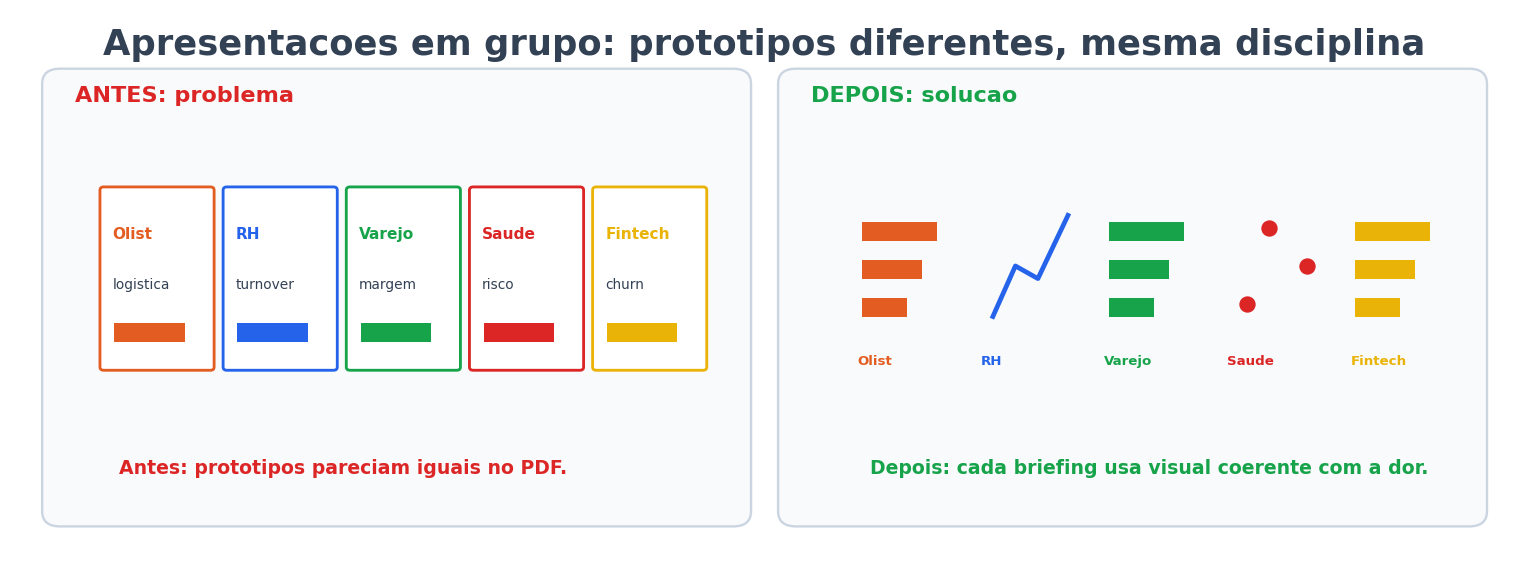
\includegraphics[width=0.62\textwidth]{semana_especial/outputs/cmp_grupos_preview.png}
\end{center}

Os protótipos HTML continuam separados por grupo (\texttt{grupo\_a.html} a \texttt{grupo\_e.html}), mas a figura acima resume a diferença esperada entre eles: cada briefing deve ter visual próprio, coerente com a dor de negócio, e não uma cópia do mesmo layout com dados trocados.
% -------------------------------------------------------

\subsection{Grupo 1 --- E-commerce (Olist)}

\textbf{Dataset:} Brazilian E-Commerce Public Dataset (Olist)\\
\url{https://www.kaggle.com/datasets/olistbr/brazilian-ecommerce}

\textbf{Dor:} atrasos na entrega derrubam as avaliações dos clientes e aumentam o churn de vendedores parceiros da plataforma.

\textbf{Pergunta 1:} ``Em quais estados e categorias os atrasos são mais críticos e qual o impacto nas avaliações (review\_score)?'' \quad \textbf{Pergunta 2:} ``Como o tempo de entrega em dias se correlaciona com a avaliação do cliente?''

\textbf{Big Idea sugerida:} ``Eletrônicos em SP concentram 34\% dos atrasos e puxam o review médio para 3,2 estrelas --- priorizar logística nessa categoria pode elevar o review para 4,1 e reduzir o churn de vendedores em 15\%.'' \quad \textbf{Call to Action:} redesenhar a rota logística de Eletrônicos em SP até Q3/2026.

\textbf{Transformações necessárias:} (1) Join: \texttt{orders $\bowtie$ order\_items $\bowtie$ products $\bowtie$ customers} (chave: \texttt{order\_id} e \texttt{product\_id}). (2) Campo: \texttt{delivery\_delay = order\_delivered\_customer\_date $-$ order\_estimated\_delivery\_date}. (3) Flag: \texttt{is\_late = IF delivery\_delay > 0 THEN ``Atrasado'' ELSE ``No Prazo'' END}. (4) Traduzir categorias com \texttt{product\_category\_name\_translation.csv}. (5) Filtrar status \texttt{canceled} e \texttt{unavailable}.

\textbf{Sheets:} (1) Big Number (\% atrasados por estado/categoria). (2) Mapa coroplético: estado $\times$ \% atraso. (3) Barras horizontais: Top 10 categorias $\times$ \% atraso, líder em laranja. (4) Scatter: dias de atraso $\times$ review\_score + linha de tendência. (5) Linha temporal de atrasos por mês. \textbf{Protótipo HTML:} \texttt{semana\_especial/grupo\_a.html}.

\subsection{Grupo 2 --- People Analytics (IBM HR)}

\textbf{Dataset:} IBM HR Analytics Employee Attrition\\
\url{https://www.kaggle.com/datasets/pavansubhasht/ibm-hr-analytics-attrition-dataset}

\textbf{Dor:} turnover de 28\% em TI custa R\$450k/ano em recrutamento e perda de conhecimento institucional.

\textbf{Pergunta 1:} ``Qual perfil de funcionário tem maior risco de saída e em qual departamento o problema é mais crítico?'' \quad \textbf{Pergunta 2:} ``Satisfação no trabalho e faixa salarial influenciam o turnover?''

\textbf{Big Idea:} ``Funcionários de TI com menos de 2 anos e sem promoção nos últimos 3 anos têm 3$\times$ mais chance de sair --- mentoria focada nesse perfil pode reduzir o turnover de 28\% para 15\% e economizar R\$270k/ano.''

\textbf{Transformações:} (1) \texttt{Attrition\_Num = IF [Attrition]=``Yes'' THEN 1 ELSE 0 END}. (2) \texttt{Turnover\_Rate = AVG(Attrition\_Num) * 100}. (3) Bins de salário (Baixo $<$ 3k / Médio 3k--7k / Alto $>$ 7k). (4) \texttt{Perfil\_Risco = IF [YearsAtCompany] < 2 AND [YearsSinceLastPromotion] > 2 THEN ``Alto Risco'' END}.

\textbf{Sheets:} Big Number (turnover TI vs meta 15\%); barras por departamento com linha de meta; heatmap satisfação $\times$ faixa salarial $\times$ turnover; scatter anos na empresa $\times$ turnover; bullet chart por departamento. \textbf{Protótipo HTML:} \texttt{semana\_especial/grupo\_b.html}.

\subsection{Grupo 3 --- Varejo (Superstore)}

\textbf{Dataset:} Sample Superstore Dataset\\
\url{https://www.kaggle.com/datasets/vivek468/superstore-dataset-final}

\textbf{Dor:} margens negativas em Tecnologia/Sul drenam R\$120k/trimestre do lucro operacional.

\textbf{Pergunta 1:} ``Quais combinações de subcategoria e região geram prejuízo consistente?'' \quad \textbf{Pergunta 2:} ``Existe correlação entre o desconto aplicado e a margem negativa?''

\textbf{Big Idea:} ``Descontos acima de 20\% em Máquinas e Copiadoras na Região Sul concentram 73\% do prejuízo --- capear o desconto em 12\% pode reverter a margem de $-$4,2\% para $+$5,8\%, gerando R\$85k adicionais por trimestre.''

\textbf{Transformações:} (1) \texttt{Margem\_Pct = SUM([Profit]) / SUM([Sales]) * 100}. (2) Bins de desconto (Sem / 0--10\% / 10--20\% / Acima 20\%). (3) \texttt{Prejuizo = IF [Profit] < 0 THEN ``Prejuízo'' ELSE ``Lucro'' END}.

\textbf{Sheets:} Big Number (margem Tech/Sul vs parâmetro de meta 8\%); mapa de calor subcategoria $\times$ região; scatter desconto $\times$ lucro com linhas de referência (0 no eixo Y; 20\% no eixo X); barras agrupadas por região; linha trimestral de margem. \textbf{Protótipo HTML:} \texttt{semana\_especial/grupo\_c.html}.

\subsection{Grupo 4 --- Saúde Pública (Heart Disease)}

\textbf{Dataset:} Heart Disease UCI Dataset\\
\url{https://www.kaggle.com/datasets/johnsmith88/heart-disease-dataset}

\textbf{Dor:} doenças cardíacas = 38\% das internações municipais (custo médio R\$12k/internação).

\textbf{Pergunta 1:} ``Quais fatores de risco têm maior correlação com diagnóstico de doença cardíaca?'' \quad \textbf{Pergunta 2:} ``Qual faixa etária e perfil clínico priorizar em campanhas preventivas?''

\textbf{Big Idea:} ``Colesterol $>$ 240 + pressão arterial $>$ 140 + idade $>$ 55 anos identificam 73\% dos casos de alto risco com apenas 3 variáveis --- triagem preventiva focada nesse perfil pode reduzir internações em 25\% e gerar R\$2,1M de economia anual.''

\textbf{Transformações:} (1) \texttt{Diagnostico = IF [target]=1 THEN ``Doença'' ELSE ``Sem Doença'' END}. (2) \texttt{Sexo = IF [sex]=1 THEN ``Masculino'' ELSE ``Feminino'' END}. (3) Bins de faixa etária ($<$45 / 45--54 / 55--64 / 65+). (4) \texttt{Perfil\_Risco = IF [chol]>240 AND [trestbps]>140 AND [age]>55 THEN ``Alto Risco'' END}. (5) \texttt{Taxa\_Doenca = AVG([target]) * 100}.

\textbf{Sheets:} Big Number (taxa doença em homens $>$ 55); barras de correlação por fator; heatmap faixa etária $\times$ perfil $\times$ taxa; scatter colesterol $\times$ pressão (cor = diagnóstico, linhas em 240 e 140); boxplot de idade por grupo. \textbf{Protótipo HTML:} \texttt{semana\_especial/grupo\_d.html}.

\subsection{Grupo 5 --- Fintech (Credit Card Churn)}

\textbf{Dataset:} Credit Card Customers Dataset\\
\url{https://www.kaggle.com/datasets/sakshigoyal7/credit-card-customers}

\textbf{Dor:} churn de cartão Premium custa R\$2,1M/ano em receita perdida de juros e anuidade.

\textbf{Pergunta 1:} ``Qual perfil de cliente Premium tem maior propensão ao cancelamento?'' \quad \textbf{Pergunta 2:} ``Frequência de uso e limite de crédito influenciam significativamente o churn?''

\textbf{Big Idea:} ``Clientes Premium com limite $<$ R\$10k e menos de 20 transações/ano têm 4$\times$ mais chance de cancelamento --- engajamento proativo focado nesse perfil pode preservar R\$1,2M em receita anual.''

\textbf{Transformações:} (1) \texttt{Churned = IF [Attrition\_Flag]=``Attrited Customer'' THEN 1 ELSE 0 END}. (2) \texttt{Churn\_Rate = AVG(Churned) * 100}. (3) Bins de limite ($<$ R\$10k / R\$10k--30k / $>$ R\$30k). (4) Bins de uso (Baixa $<$ 20 trans / Média 20--50 / Alta $>$ 50). (5) \texttt{Perfil\_Risco = IF [Total\_Trans\_Ct] < 20 AND [Credit\_Limit] < 10000 THEN ``Alto Risco'' END}.

\textbf{Sheets:} Big Number (churn Premium com limite $<$ R\$10k vs benchmark 8\%); barras faixa de limite $\times$ churn; scatter frequência $\times$ valor médio (cor = churn, linha em 20 transações); linha temporal de churn por segmento; heatmap frequência $\times$ limite $\times$ taxa de churn. \textbf{Protótipo HTML:} \texttt{semana\_especial/grupo\_e.html}.

% -------------------------------------------------------
\section{Rubrica de Avaliação --- Apresentação em Grupo}
% -------------------------------------------------------

\begin{tabular}{|p{4.5cm}|r|p{7.5cm}|}
\hline
\textbf{Critério} & \textbf{Peso} & \textbf{Descrição} \\
\hline
Big Idea + Call to Action & 15\% & Explicitada no pitch: ponto de vista + tensão + stake \\
Estrutura do dashboard   & 20\% & Pergunta $\to$ Big Number + Insight IA $\to$ Gráficos $\to$ Tabela \\
Qualidade dos visuais    & 20\% & Títulos-mensagem; cor com propósito; sem chartjunk \\
Insight IA               & 15\% & Acionável; não genérico; ao lado do Big Number \\
Tableau funcional        & 15\% & $\geq$ 1 filtro ou parâmetro funcionando \\
Pitch de 3 minutos       & 15\% & SCR completo; dentro do tempo; call to action explícito \\
\hline
\textbf{Total}           & \textbf{100\%} & \\
\hline
\end{tabular}

% \includegraphics paths são relativos ao diretório de main.tex (aula/)
% =============================================================================

\chapter{Semana Especial (04/05 + 18/05/2026)\\[4pt]Revisão Unidade~II e Dashboard em Grupo}

Este impresso cobre as duas últimas aulas antes das provas. No dia \textbf{04/05} fazemos a revisão de toda a Unidade~II. No dia \textbf{18/05} cada grupo apresenta o dashboard no Tableau --- como está descrito na Parte~III deste documento, que você já recebe hoje para ter duas semanas de preparo. As provas começam na semana de \textbf{25/05}.

% ============================================================
\section*{\Large PARTE I --- REVISÃO DA UNIDADE II (04/05/2026)}
% ============================================================

% -------------------------------------------------------
\section{AED vs.\ Análise Explanatória}
% -------------------------------------------------------

Na Unidade~I vocês exploraram dados para \emph{entender}: histogramas, boxplots, correlações, dados ausentes. A pergunta que guiava cada análise era ``o que os dados me dizem?'' A Unidade~II começa com uma mudança radical de perspectiva. A pergunta agora é outra: \textit{``como eu conto essa história para que alguém tome uma decisão?''}

Quando você sai do papel de analista e entra no papel de comunicador, você faz análise \textbf{explanatória}. A audiência mudou: não é mais você mesmo --- é o CEO, o gerente, o comitê de crédito. Essas pessoas não têm tempo para ver os 200 gráficos que você gerou. Elas precisam de uma mensagem clara suportada pelas evidências certas.

O erro mais comum de analistas iniciantes é mostrar todo o processo exploratório para uma audiência executiva. O resultado: confusão, perda de tempo, e a descoberta mais importante se perde no meio de 30 gráficos. Na análise explanatória, você já sabe a história que vai contar e escolhe \emph{apenas} os gráficos que a sustentam.

\begin{BoardBox}[title=AED vs.\ Explanatória]
\begin{tabular}{@{}lp{4.2cm}p{5.2cm}@{}}
\toprule
 & \textbf{Exploratória (AED)} & \textbf{Explanatória} \\
\midrule
Audiência & O analista & CEO, gerente, investidor \\
Objetivo  & Entender o dado & Provocar uma decisão \\
Linguagem & ``O dado mostra X'' & ``O que este dado muda no que você faz?'' \\
Visuais   & Centenas (maioria descartada) & Só os que servem à mensagem \\
\bottomrule
\end{tabular}
\end{BoardBox}

Toda vez que você estiver construindo uma apresentação, faça esta pergunta para cada gráfico: ``este visual serve à mensagem ou serve à minha curiosidade?'' Se for a segunda opção, ele vai para o apêndice.

\begin{center}
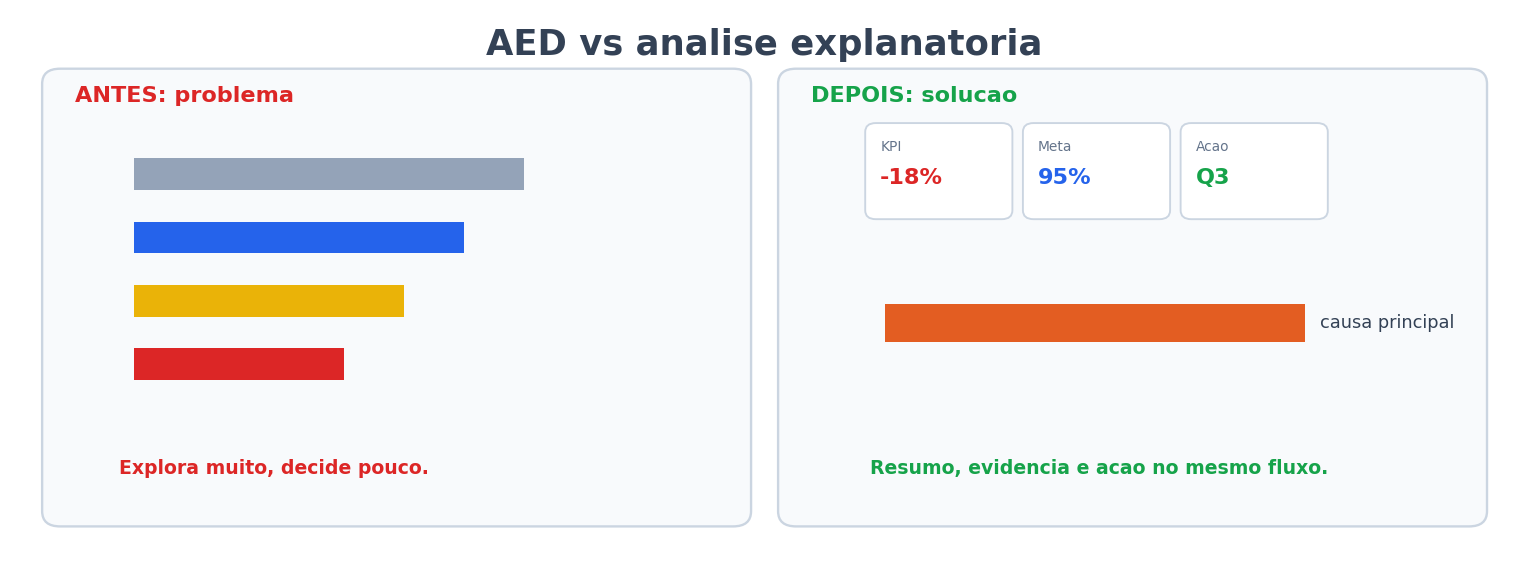
\includegraphics[width=0.58\textwidth]{semana_especial/outputs/cmp_cap2_aed_explanatoria.png}
\end{center}

\textbf{Exemplo prático:} você está analisando dados de alunos em uma instituição de ensino. Na perspectiva exploratória, você gera: correlação entre horas estudadas e nota (0,58), distribuição de notas por sexo, boxplot por disciplina, análise de outliers, falta versus nota. Tudo isso é válido para \emph{você entender} o dado. Mas quando você entra em uma reunião com o diretor e tem 10 minutos, você escolhe apenas \textbf{uma} visualização: alunos com envolvimento familiar baixo + menos de 15 horas de estudo têm nota 9 pontos abaixo da média. Isso é explanatória. A pergunta que o diretor responde depois de ver esse gráfico não é ``que curioso'' --- é ``o que fazemos para resgatar esses alunos?''

% -------------------------------------------------------
\section{Big Idea Framework}
% -------------------------------------------------------

A Big Idea é \textbf{uma única frase} que captura a essência da sua mensagem. Nancy Duarte, em \textit{Datastory} (2019), define que toda boa apresentação de dados deve ter uma Big Idea que a pessoa leva para casa mesmo sem ter visto nenhum gráfico. Ela é o título do seu argumento --- não do seu relatório.

Ela exige três componentes: (1) um \textbf{ponto de vista} --- uma afirmação, não uma observação neutra; (2) a \textbf{tensão} --- o que está em jogo se nada for feito; (3) o \textbf{stake} --- por que a audiência deveria se importar. A fórmula prática é: [recomendação de ação] + [dado concreto que justifica] + [impacto se nada mudar].

\begin{BoardBox}[title=Big Idea --- 3 Componentes e Fórmula]
\begin{enumerate}
  \item \textbf{Ponto de vista:} afirmação, não observação.
  ``O dado mostra X'' \textrightarrow{} não é Big Idea.
  ``Devemos fazer Y porque X'' \textrightarrow{} é Big Idea.
  \item \textbf{Tensão:} o que está em jogo? Risco de não agir?
  \item \textbf{Stake:} por que a audiência deveria se importar?
\end{enumerate}
\smallskip
\textbf{Fórmula:} [ação recomendada] + [dado que justifica] + [impacto financeiro/operacional]
\end{BoardBox}

Veja a diferença: ``A taxa de cancelamento subiu 12\%'' é uma observação --- não orienta nenhuma decisão. ``Se não corrigirmos o onboarding até setembro, perderemos R\$1,2M em receita recorrente nos próximos 12 meses'' tem ponto de vista (corrigir o onboarding), tensão (se não fizermos nada) e stake (R\$1,2M). Essa frase é Big Idea.

O \textbf{teste}: leia para alguém que não viu os dados. Se a resposta for ``interessante'' sem que a pessoa saiba o que fazer --- a Big Idea não está pronta. Ela deve provocar a pergunta ``e como a gente faz isso?''

\begin{center}
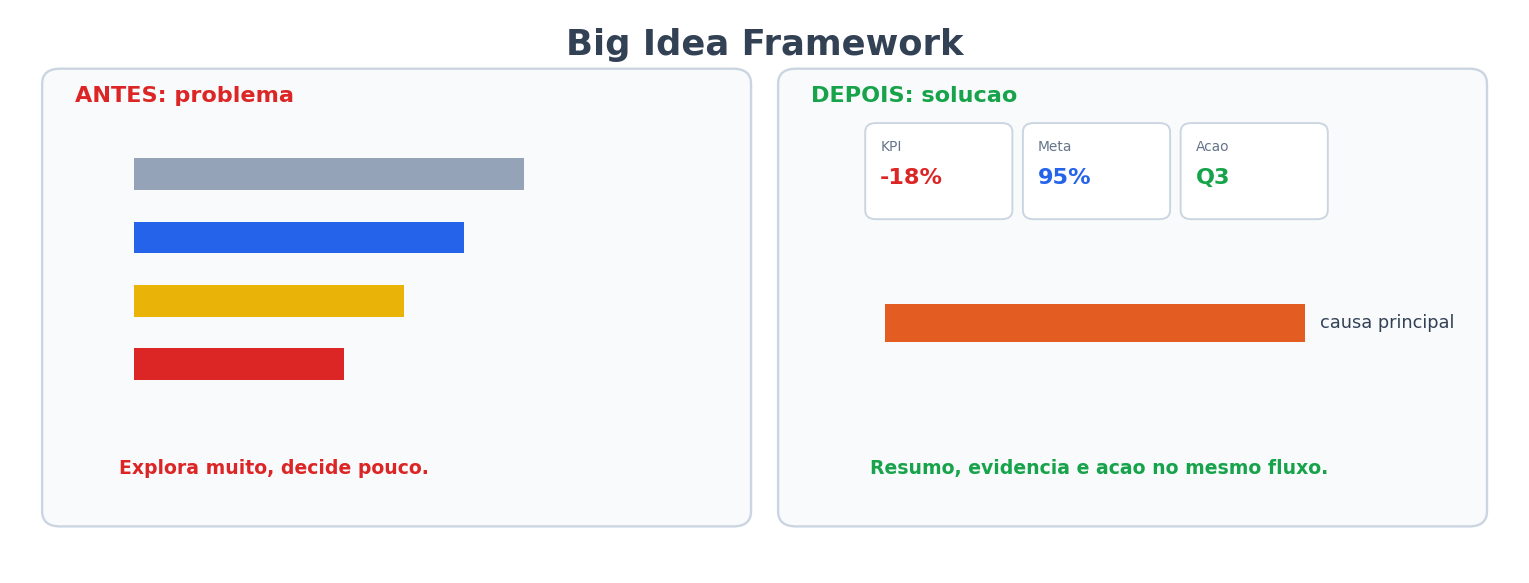
\includegraphics[width=0.58\textwidth]{semana_especial/outputs/cmp_cap2_big_idea.png}
\end{center}

Toda Big Idea está ligada a uma \textbf{pergunta de decisão}: a questão que a audiência precisa responder ao final. Exemplos: ``Devemos expandir para o canal digital ou reforçar o físico?''; ``Qual produto descontinuamos no Q3?''. O analista não precisa ter a resposta --- mas deve apresentar os dados que tornam a resposta possível.

\textbf{Mais exemplos de Big Ideas em diferentes domínios:}
\begin{itemize}
  \item \textit{E-commerce:} ``Frete grátis acima de R\$100 aumenta o ticket médio em 34\%, mas reduz a margem em apenas 8\% --- implementar já seria rentável no Q3.''
  \item \textit{RH:} ``Desenvolvedores sem promoção em 3 anos têm 5$\times$ mais chance de sair; implementar plano de carreira acelerado para 23 talentos preservaria R\$480k em custos de reposição anual.''
  \item \textit{Saúde:} ``Pacientes que recebem chamada de lembrete 24h antes da consulta aumentam a taxa de comparecimento em 41\%; reduz custos operacionais em R\$120k/ano.''
\end{itemize}

\textbf{Teste na prática:} leia sua Big Idea para um colega que não mexe com seus dados. Se ele disser ``muito interessante'', ela ainda não está pronta. Se ele disser ``e quando a gente começa?'', pronto --- você tem uma Big Idea de verdade.

% -------------------------------------------------------
\section{Storyboard e Estrutura Narrativa}
% -------------------------------------------------------

Antes de abrir o Tableau e construir qualquer gráfico, você desenha o \textbf{storyboard} --- um rascunho em papel com os títulos das telas e o tipo de visual em cada uma. Ele força você a pensar na narrativa \emph{antes} de pensar nas ferramentas. Quem abre o Tableau sem storyboard constrói gráficos bonitos sem história.

Nancy Duarte propõe uma estrutura de 4 atos adaptada de narrativas clássicas. O truque é que toda boa apresentação de dados segue exatamente essa ordem: você mostra o estado atual, revela a tensão, apresenta a proposta e termina com um pedido concreto.

\begin{BoardBox}[title=Estrutura Narrativa --- 4 Atos]
\begin{enumerate}
  \item \textbf{Contexto --- O que é:} estado atual; KPIs reais; o ponto de partida.
  \item \textbf{Conflito --- O que poderia ser:} a tensão; o dado que revela o problema.
  \item \textbf{Resolução --- O que proponho:} proposta baseada em evidências.
  \item \textbf{Call to Action:} decisão pedida + responsável + prazo.
\end{enumerate}
\smallskip
\textbf{Em telas:} KPIs atuais \textrightarrow{} problema \textrightarrow{} análise/evidências \textrightarrow{} recomendação
\end{BoardBox}

Cada tela do storyboard deve ter: (1) título que é mensagem --- não ``Gráfico de Barras'', mas sim ``Canal físico custa 4$\times$ mais por venda''; (2) tipo de visual proposto; (3) esboço manual do dado; (4) transição lógica para a próxima tela, como ``por isso, na próxima tela, veja\ldots''

\begin{center}
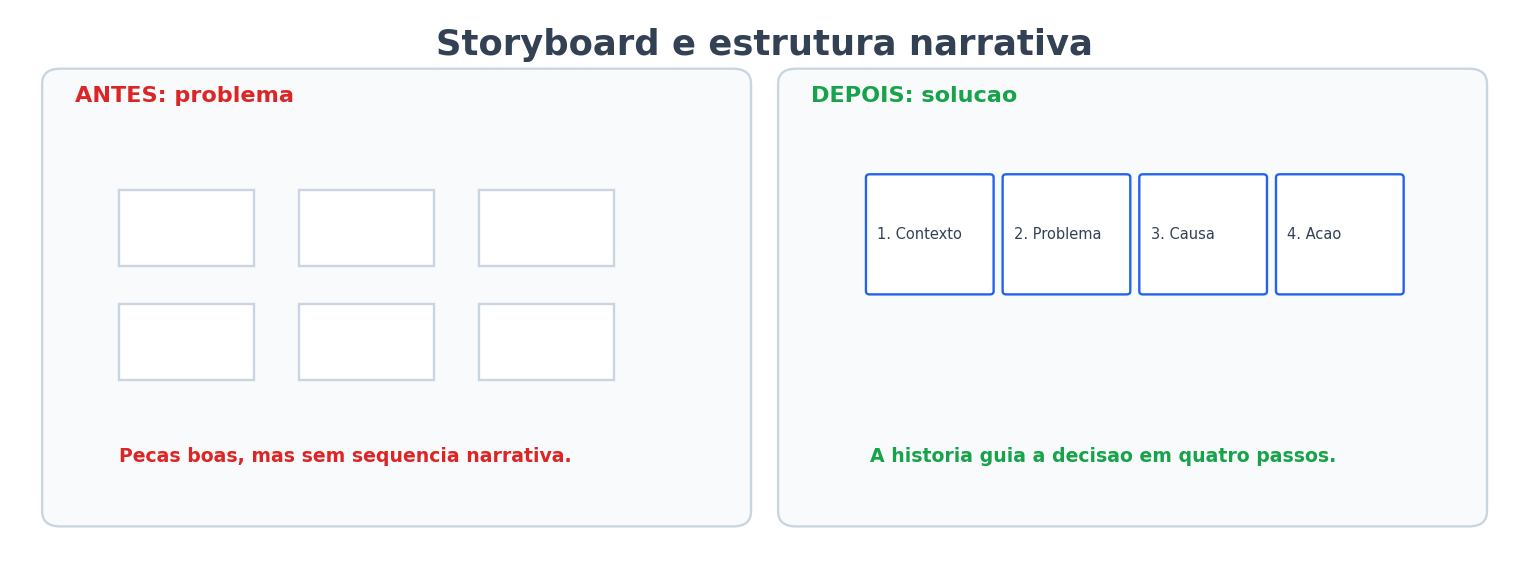
\includegraphics[width=0.58\textwidth]{semana_especial/outputs/cmp_cap2_storyboard.png}
\end{center}

\textbf{Exemplo de storyboard em 4 telas de uma apresentação executiva:}
\begin{enumerate}
  \item \textbf{Tela 1 --- Contexto:} ``Vendas em regiões Sul e Centro-Oeste crescem 15\% acima da média nacional.'' (Big Number destacado + KPI) Transição: ``mas quando olhamos a margem, a história muda radicalmente.''
  \item \textbf{Tela 2 --- Conflito:} ``Essas mesmas regiões têm margem negativa em Tecnologia.'' (Scatter: Desconto vs Margem, cor vermelho no quadrante negativo) Transição: ``achamos 3 subcategorias que concentram 73\% do prejuízo.''
  \item \textbf{Tela 3 --- Análise:} ``Máquinas em SP têm desconto médio de 26\%; Copiadoras em Sul, 23\%; comparando com Nordeste (14\%), o culpado é a política de desconto regional.'' (Tabela + box destacando as 3 categorias críticas) Transição: ``por isso recomendamos\ldots''
  \item \textbf{Tela 4 --- Recomendação:} ``Capar desconto máximo em 12\% em Tecnologia/Sul até 01/junho recupera R\$85k de margem trimestral e move o resultado de -4,2\% para +5,8\%.'' (Simulação com 3 cenários: otimista, realista, pessimista) Próximo passo: ``Gerência Comercial, confirmar a implementação até 15/maio?''
\end{enumerate}

O storyboard em papel \textbf{antes de você abrir o Tableau} economiza semanas de trabalho. Você já sabe qual série temporal é importante, qual drill-down você precisa, quantas telas usará. Quem pula essa etapa muitas vezes constrói um dashboard tecnicamente correto mas narrativamente confuso.

% -------------------------------------------------------
\section{Design de Informação: Pré-atenção e Atributos Visuais}
% -------------------------------------------------------

Antes de você ler deliberadamente qualquer coisa num gráfico, seu cérebro já detectou alguns elementos em menos de 250 milissegundos, sem esforço consciente. Esses são os \textbf{atributos pré-atencionais}. Se você os usa para destacar o que importa, o leitor chega à mensagem antes de ler o título. Se os usa aleatoriamente, o leitor fica desorientado.

A regra de ouro é usar no máximo \textbf{dois atributos pré-atencionais} por visual. Acima disso, a hierarquia colapsa e o olho não sabe onde pousar.

\begin{BoardBox}[title=Atributos Pré-atencionais]
\begin{tabular}{@{}llp{5.2cm}@{}}
\toprule
\textbf{Atributo} & \textbf{Função} & \textbf{Regra de uso} \\
\midrule
Cor        & Destaca, agrupa       & 1 cor de destaque; resto em cinza neutro \\
Tamanho    & Indica magnitude      & Maior = mais importante; consistência obrigatória \\
Posição    & Organiza hierarquia   & Mais importante: canto superior esquerdo \\
Intensidade & Contraste claro/escuro & Mais escuro = mais importante \\
Enclosure  & Agrupa elementos      & Caixa ao redor de dados relacionados \\
\bottomrule
\end{tabular}
\end{BoardBox}

A \textbf{cor} merece atenção especial. Há a cor semântica (vermelho = alerta, verde = ok, amarelo = atenção) e a cor de destaque (uma cor viva para o elemento que carrega a mensagem; todo o resto em cinza). Use cor semântica onde já existe convenção estabelecida. Nunca inverta vermelho e verde sem motivo forte. E lembre: 8\% dos homens têm daltonismo vermelho-verde --- evite que essa combinação seja o único diferenciador.

\begin{center}
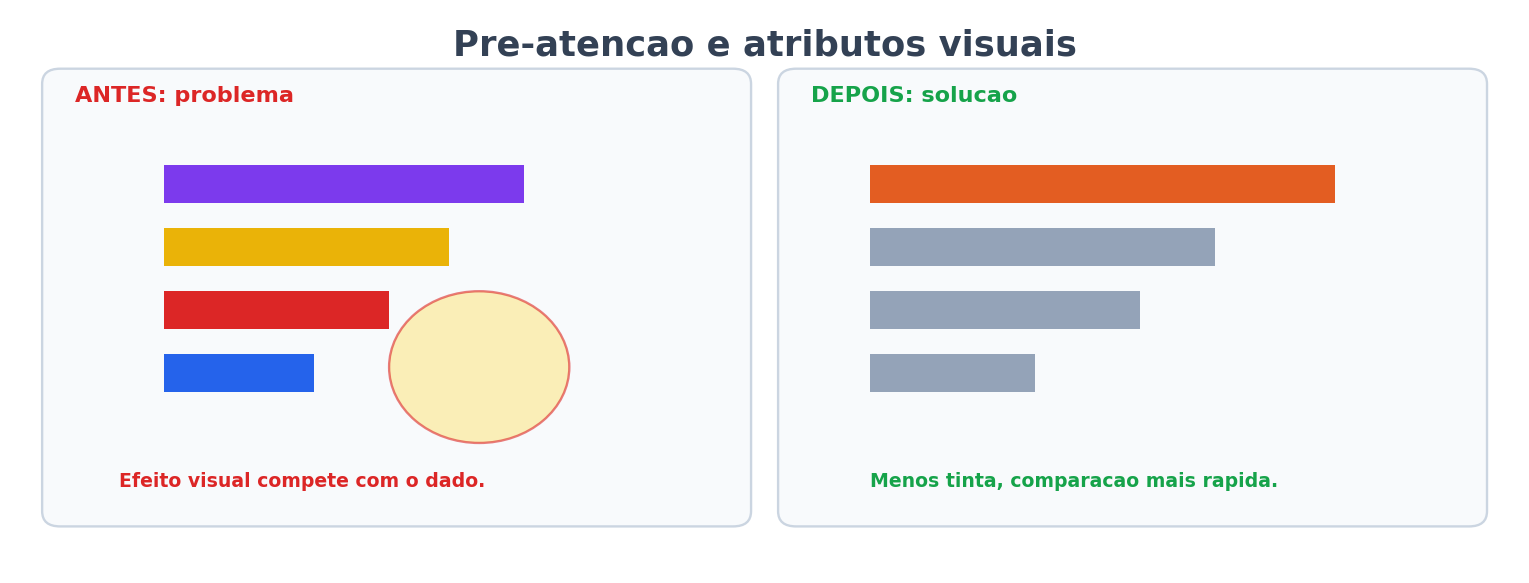
\includegraphics[width=0.58\textwidth]{semana_especial/outputs/cmp_cap2_preatencao.png}
\end{center}

\textbf{Regra de ouro revisitada:} você consegue usar até 2 atributos pré-atencionais em harmonia. Exemplo: na ábaco visual mostrando performance por time, use \textbf{COR} para semântica (verde = meta atingida, vermelho = abaixo) e \textbf{TAMANHO} para magnitude (bolinha grande = time grande, bolinha pequena = time pequeno). Juntos, os dois atributos permitem decodificação instantânea. Se você adicionar um terceiro --- posição espacial não óbvia, ou intensidade de padrão --- o cérebro fica sobrecarregado e falha no teste do relance. Na prática, quando você entra na dúvida de ``será que está confuso?'', sempre está. Remova o terceiro atributo.

% -------------------------------------------------------
\section{Teste do Relance e Título-Mensagem}
% -------------------------------------------------------

O Teste do Relance é simples: mostre o gráfico por 3 segundos, cubra e pergunte à audiência o que viram e qual a mensagem principal. Se não conseguirem responder em 3 segundos, o visual falhou. Não o leitor --- o design.

\begin{BoardBox}[title=Teste do Relance --- Diagnóstico de Falha]
Causas mais comuns de falha:
\begin{itemize}
  \item Título rótulo em vez de título mensagem
  \item Excesso de elementos --- o olho não sabe onde pousar
  \item Cores sem propósito --- todas as barras em cores diferentes
  \item Legenda separada --- o leitor desvia o olhar para decodificar
\end{itemize}
\smallskip
\textbf{Fórmula do título mensagem:} [Sujeito] + [verbo de tendência] + [magnitude]\\
Ex.: ``Churn \textbf{caiu} 34\% após o programa de fidelidade''
\end{BoardBox}

A diferença entre título rótulo e título mensagem é a diferença entre ``Vendas por Região'' e ``Região Sul concentra 58\% das vendas''. O primeiro descreve o que o eixo mostra. O segundo já entrega a informação. Para o executivo com 5 minutos por dia, o título mensagem é o gráfico mais importante --- porque ele consegue ler apenas os títulos e já sabe o que decidir.

\begin{center}
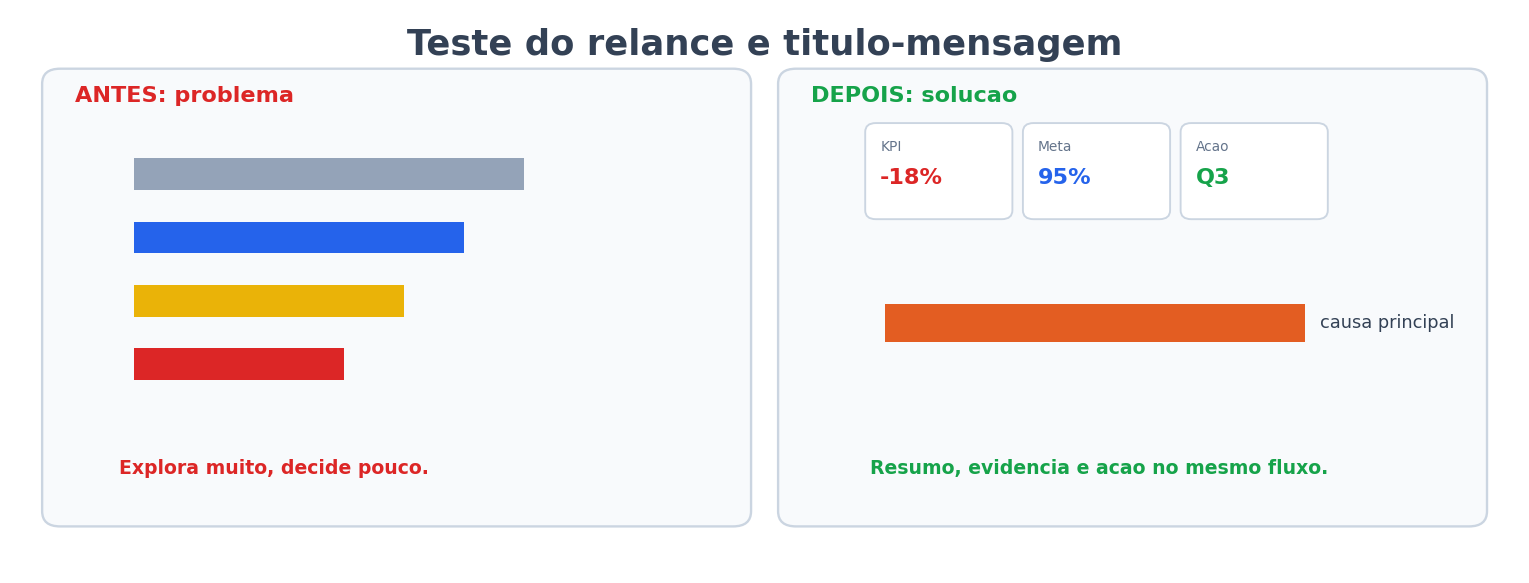
\includegraphics[width=0.58\textwidth]{semana_especial/outputs/cmp_cap2_relance.png}
\end{center}

\textbf{Checklist para passar no Teste do Relance:} (1) título é mensagem, não rótulo? (2) cores comunicam semântica ou prioridade, não decoração? (3) gráfico tem exatamente 1 ou 2 atributos pré-atencionais, não mais? (4) sem ambiguidade: alguém que não viu o dado sabe imediatamente qual a mensagem?

Quando você apresenta um dashboard para alguém pela primeira vez, teste na prática: mostre por 3 segundos, tape a tela e pergunte ``qual a mensagem principal deste gráfico?'' Se a resposta não estiver clara, você ainda tem trabalho. Se estiver absolutamente cristalina --- pronto, passou.

% -------------------------------------------------------
\section{Data-Ink Ratio e Chartjunk}
% -------------------------------------------------------

Edward Tufte (1983) propõe o conceito de \textbf{data-ink ratio}: a proporção da tinta do gráfico que realmente representa dados sobre a tinta total. Maximize esse ratio. Tudo que ocupa tinta sem carregar informação é candidato à remoção.

\begin{BoardBox}[title=Data-Ink Ratio e Chartjunk]
\[
  \text{Data-ink ratio} = \frac{\text{tinta que representa dados}}{\text{tinta total do gráfico}}
\]
\textbf{Chartjunk --- remova:} grades pesadas $\cdot$ barras 3D $\cdot$ sombras $\cdot$ gradientes decorativos $\cdot$ legendas redundantes $\cdot$ ícones temáticos $\cdot$ mais de 3 casas decimais\\[4pt]
\textbf{Princípio:} ``Se eu remover isso, o gráfico fica menos claro?'' Se não --- remova.
\end{BoardBox}

O gráfico de pizza com 8 fatias em 8 cores é o exemplo clássico de chartjunk. O olho humano não compara ângulos com precisão; ele compara comprimentos. Substitua pizza por barras horizontais ordenadas, com 1 cor de destaque para a categoria que carrega a mensagem e rótulos diretos nas barras --- elimine a legenda.

\begin{center}
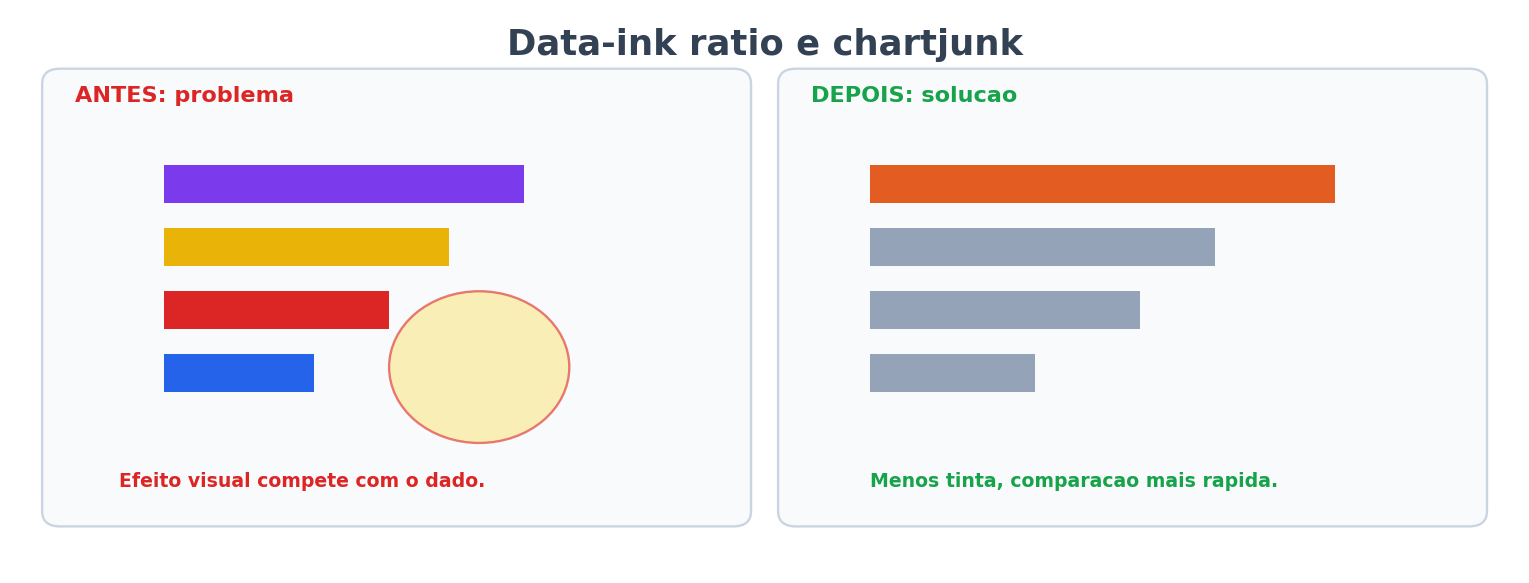
\includegraphics[width=0.58\textwidth]{semana_especial/outputs/cmp_cap2_chartjunk.png}
\end{center}

\textbf{Exemplo de eliminação de chartjunk em 3 passos:} Você tem um gráfico de barras com: (1) grid pesado horizontal e vertical (remove); (2) barras com borda preta (remove); (3) sombra abaixo das barras (remove); (4) legenda no lado dizendo ``Série 1'' (remove --- coloque o rótulo direto na barra); (5) números com 3 casas decimais (reduz para 1 ou 2). Resultado final: data-ink ratio sobe de 50\% para 85\%, o gráfico fica 70\% menor em tamanho visual, e a mensagem fica mais clara.

Em Tableau, a regra é simples: remova toda grid, remova border das marcas, use espaçamento generoso, e ative os rótulos diretos. O resultado é um visual que cabe em uma tela de executivo sem parecer ``deserto''.

% -------------------------------------------------------
\section{Tableau: Filtros, Parâmetros e Ações}
% -------------------------------------------------------

Dois recursos fundamentais de interatividade no Tableau que os alunos frequentemente confundem. A diferença é direta: \textbf{filtros} incluem ou excluem linhas do dataset; \textbf{parâmetros} mudam o cálculo sem filtrar nenhuma linha. Um filtro por estado exibe só os dados de PE --- os dados de SP desaparecem da view. Um parâmetro de métrica permite que o usuário escolha entre Receita ou Margem --- nenhum dado é excluído, apenas o campo calculado muda.

\begin{BoardBox}[title=Filtros vs.\ Parâmetros]
\begin{tabular}{@{}lp{4.5cm}p{5.2cm}@{}}
\toprule
 & \textbf{Filtro} & \textbf{Parâmetro} \\
\midrule
Função   & Inclui/exclui linhas      & Muda o cálculo \\
Uso      & Selecionar região, categoria & Alternar métrica, definir meta, Top N \\
Exemplo  & ``Ver só PE''             & ``Exibir Receita ou Margem?'' \\
\bottomrule
\end{tabular}
\smallskip

\textbf{Campo calculado com parâmetro:}\\
\texttt{IF [Vendas] >= [Meta] THEN ``Atingiu'' ELSE ``Abaixo'' END}
\end{BoardBox}

Sobre a \textbf{hierarquia de filtros}: o Tableau executa filtros em ordem fixa. O mais importante para a prova é o \textbf{Context Filter}. Quando você precisa de Top~N dentro de uma região já filtrada, adicione o filtro de região como Context Filter primeiro --- senão o Tableau calcula o Top~N sobre o dataset inteiro, ignorando o filtro de região.

\begin{center}
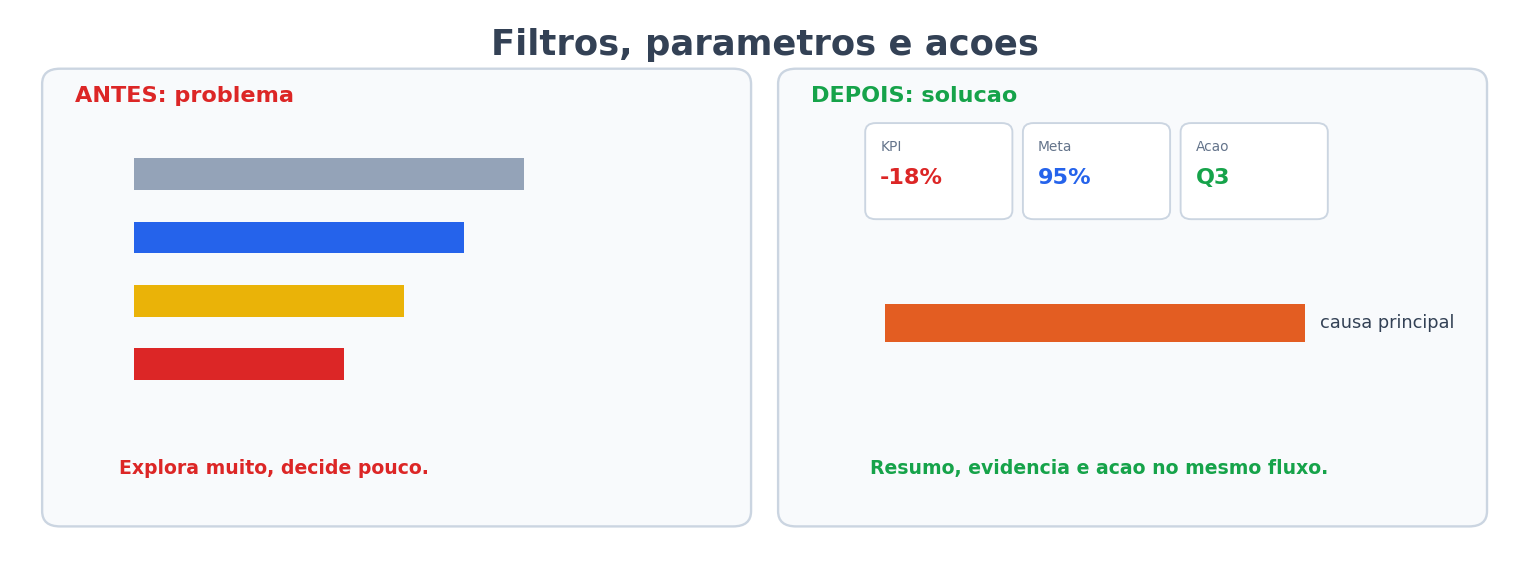
\includegraphics[width=0.58\textwidth]{semana_especial/outputs/cmp_cap2_tableau.png}
\end{center}

\textbf{Pseudocódigo Tableau para parâmetros:} você cria um parâmetro chamado \verb|[Métrica_Selecionada]| com opções ``Receita'', ``Margem'', ``Unidades''. Depois cria um campo calculado:
\begin{quote}\ttfamily
IF [Métrica\_Selecionada] = ``Receita'' THEN [Receita]\\
ELSEIF [Métrica\_Selecionada] = ``Margem'' THEN [Margem]\\
ELSE [Unidades] END
\end{quote}
Quando o usuário muda o parâmetro, o campo calculado avalia instantaneamente e todo o dashboard reflete a mudança. Nenhuma linha é filtrada, apenas o cálculo muda.

\textbf{Context Filter --- quando usar:} você está vendo Top 10 Produtos por Receita em São Paulo. Se você não adicionar ``Estado = SP'' como Context Filter, o Top 10 é calculado sobre TODOS os estados, depois filtrado --- resultado: pode aparecer um produto de outro estado. Com Context Filter, o Top 10 é calculado apenas em SP, garantindo que os 10 maiores de SP apareçam.

\begin{BoardBox}[title=Ações de Dashboard --- 4 Tipos]
\begin{tabular}{@{}lp{4cm}p{4.8cm}@{}}
\toprule
\textbf{Tipo}     & \textbf{O que faz}                  & \textbf{Exemplo} \\
\midrule
Filter action   & Clicar filtra outra view             & Clicar em SP filtra todos os gráficos \\
Highlight       & Destaca sem filtrar                  & Mouse em Região destaca no mapa \\
URL action      & Abre URL com dado selecionado        & Clique abre ficha no ERP \\
Navigate        & Navega entre dashboards              & KPI leva ao painel de drill-down \\
\bottomrule
\end{tabular}
\end{BoardBox}

% -------------------------------------------------------
\section{Dashboards que Forçam Decisão}
% -------------------------------------------------------

Um dashboard pode ser tecnicamente impecável e ainda assim não provocar nenhuma ação. O problema, nesse caso, é de estrutura narrativa. Um dashboard que \textbf{força uma decisão} tem três zonas distintas e em sequência.

\begin{BoardBox}[title=As 3 Zonas do Dashboard Decisório]
\textbf{Zona 1 --- Contexto:} o que está acontecendo agora? KPIs com comparação à meta ou período anterior. Lido em $<$5 segundos. Nenhuma interpretação ainda.

\textbf{Zona 2 --- Diagnóstico:} por que está acontecendo? Drill-down por produto, região, segmento. Permite formular hipóteses --- não confirmar causas.

\textbf{Zona 3 --- Recomendação:} o que fazer? 1--2 recomendações concretas com evidências. Call to Action com \emph{quem}, \emph{o quê} e \emph{até quando}.
\end{BoardBox}

Os \textbf{anti-padrões} mais comuns: (a) tudo sempre verde --- cria conforto falso e impede decisões urgentes; (b) métricas sem definição --- ``Receita'' pode ser bruta, líquida ou MRR, e sem definição explícita cada pessoa lê diferente; (c) 50~KPIs na tela inicial --- granularidade excessiva, o usuário não sabe onde olhar; (d) número isolado sem comparação --- R\$100k de vendas é ótimo ou péssimo em relação ao quê?

\begin{center}
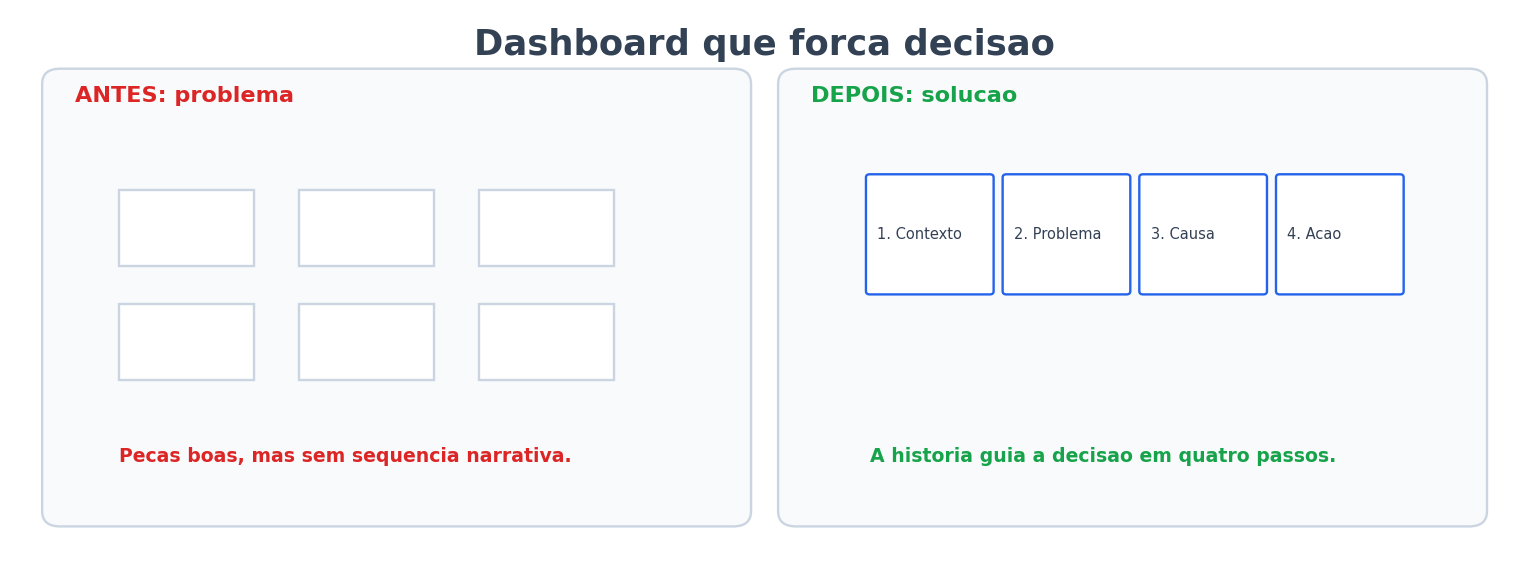
\includegraphics[width=0.58\textwidth]{semana_especial/outputs/cmp_cap2_decisorio.png}
\end{center}

\textbf{Implementação prática das 3 zonas em um dashboard de Vendas:}
\begin{itemize}
  \item \textbf{Zona 1 (Contexto):} 4 KPIs acima da dobra: (1) Receita Mês, Meta, Gap; (2) Margem %; (3) Churn; (4) NPS. Cada KPI mostra ícone de semáforo (verde/amarelo/vermelho). Tempo de leitura: <3 segundos. Nenhuma ação ainda.
  \item \textbf{Zona 2 (Diagnóstico):} 3 gráficos lado a lado: (1) Receita por Região (barras horizontais); (2) Churn vs Desconto (scatter); (3) Série temporal de Margem (linha com meta). Permite que o usuário formule hipóteses (``RJ tem desconto alto demais?'') mas não confirma causas.
  \item \textbf{Zona 3 (Recomendação):} 1 caixa destacada em cor de alerta: ``RJ concentra 65\% da receita mas margem negativa. Reduzir desconto de 26\% para 12\% recupera R\$85k trimestral sem impactar volume (elasticidade = 0,34). Gerência Comercial: implementar até 30/junho.''
\end{itemize}

\textbf{Teste de efetividade:} se seu gerente consegue ler apenas a Zona 3 e já tem uma decisão clara e acionável, sua estrutura funcionou. Se ele precisa voltar para a Zona 2 para entender, significa que a Recomendação não está autossuficiente.

% -------------------------------------------------------
\section{KPIs com Meta, Gap e Tendência}
% -------------------------------------------------------

Um KPI sozinho não decide nada. Para forçar uma decisão, ele precisa de cinco componentes. O número isolado responde ``qual é o valor?'' mas não responde ``isso é bom ou ruim?'' nem ``a situação está melhorando ou piorando?''

\begin{BoardBox}[title=Anatomia de um KPI Decisório]
\begin{enumerate}
  \item \textbf{Valor atual} --- o número real do período
  \item \textbf{Meta (target)} --- o que deveria ser
  \item \textbf{Gap} --- distância em valor absoluto e percentual
  \item \textbf{Tendência} --- seta de alta/baixa ou sparkline
  \item \textbf{Período} --- MTD, YTD, vs ano anterior
\end{enumerate}
\smallskip
\textbf{Bullet chart} (Stephen Few): barra real + barra de meta. Mais informação por cm$^2$ do que qualquer velocímetro ou gauge.
\end{BoardBox}

\begin{center}
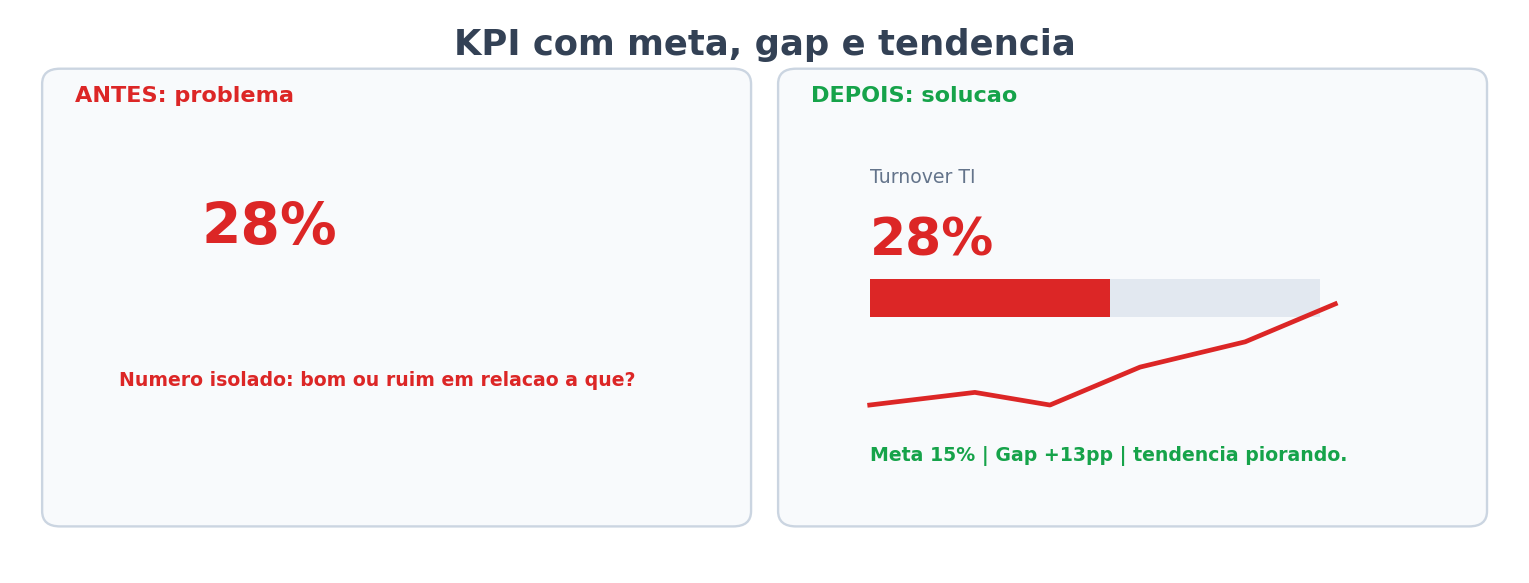
\includegraphics[width=0.58\textwidth]{semana_especial/outputs/cmp_cap2_kpi.png}
\end{center}

\textbf{Exemplos de KPIs bem estruturados em diferentes domínios:}
\begin{itemize}
  \item \textit{E-commerce:} Taxa de Retorno 8\% (Meta: 5\%, Gap: +3pp, Tendência: queda, melhorando, Período: YTD 2026)
  \item \textit{RH:} Turnover TI 28\% (Meta: 15\%, Gap: +13pp, Tendência: alta, piorando, Período: últimos 12 meses)
  \item \textit{Saúde:} Taxa de Readmissão 6,5\% (Meta: 5\%, Gap: +1,5pp, Tendência: alta, piorando, Período: YTD 2026)
\end{itemize}

Quando você tem espaço, a \textbf{bullet chart} (Stephen Few, 2006) é superior ao gauge ou velocímetro porque mostra valor atual, meta, faixa de desempenho bom/médio/ruim, tudo em uma linha horizontal. Se você tiver apenas espaço para um cartão quadrado, use: número grande + meta + gap colorido + sparkline de tendência.

\textbf{Anti-padrão a evitar:} número isolado na tela. Sempre sempre sempre colocar número com: (1) meta ou benchmark; (2) período; (3) tendência. Caso contrário, o número não informa nada --- pode ser bom, ruim, normal. O contexto é o que faz um número virar insight.

% -------------------------------------------------------
\section{Pitch de 3 Minutos}
% -------------------------------------------------------

Três minutos são aproximadamente 450 palavras. Isso é suficiente para convencer alguém --- se e somente se você seguir a estrutura certa. A estrutura SCR (Situação, Complicação, Resolução) tem quatro blocos com tempos definidos.

\begin{BoardBox}[title=Pitch de 3 Minutos --- Estrutura SCR]
\begin{enumerate}
  \item \textbf{Situação (30s):} contexto factual. Comece com o dado impactante, não com introdução genérica.
  \item \textbf{Complicação (45s):} o problema ou oportunidade revelado. Aqui entra a Big Idea.
  \item \textbf{Resolução (60s):} evidência + recomendação com número concreto. Não ``melhorar'' --- sim ``aumentar em 15\%''.
  \item \textbf{Próximo passo (45s):} pedido específico com \textit{verbo + quem + prazo}.
\end{enumerate}
\end{BoardBox}

O erro mais comum: começar com contexto genérico (``vivemos em uma era de dados\ldots'') em vez do dado que mais surpreende. Se você tem 3 minutos e gasta 30 segundos com introdução desnecessária, perdeu 17\% do tempo e a atenção da audiência.

\begin{center}
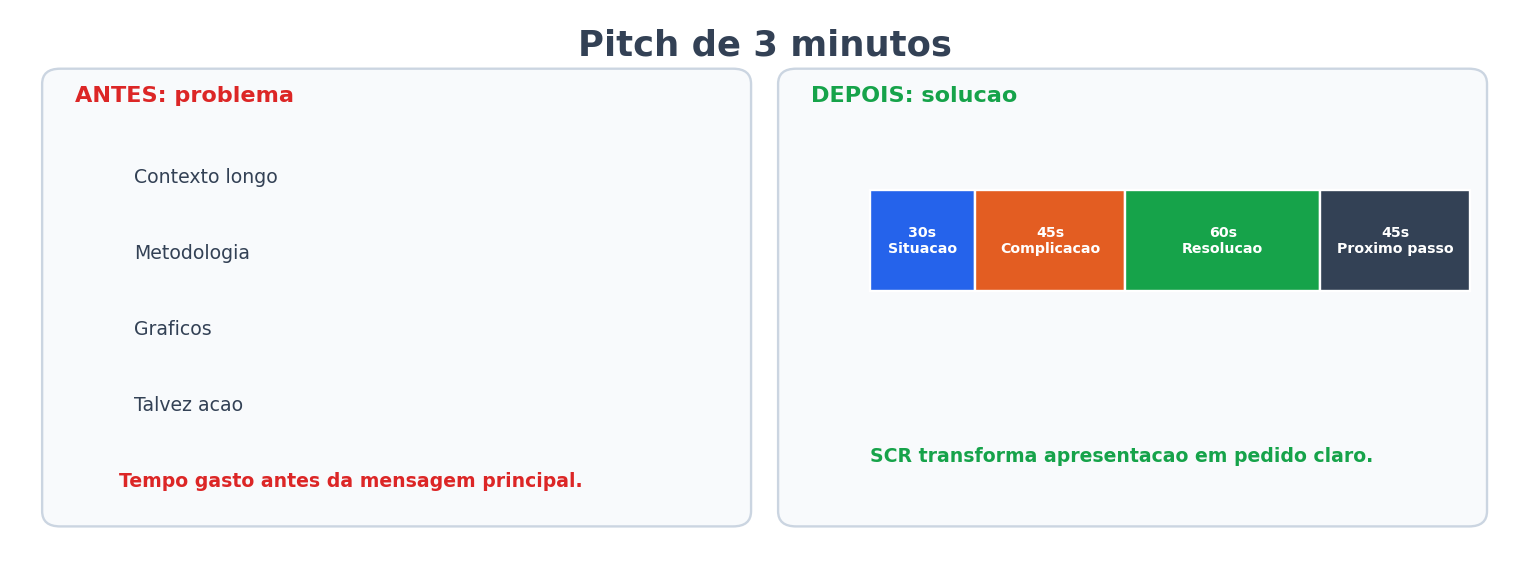
\includegraphics[width=0.58\textwidth]{semana_especial/outputs/cmp_cap2_pitch.png}
\end{center}

\textbf{Exemplo de pitch de 3 minutos em contexto acadêmico:}\\[2pt]
\textbf{Situação (30s):} ``6.607 alunos. 27\% têm nota final menor que 60. Isso significa 1.800 alunos em recuperação, triplicando a carga administrativa e reduzindo a taxa de aprovação final.''\\[2pt]
\textbf{Complicação (45s):} ``Descobrimos que esses alunos compartilham um perfil comum: envolvimento familiar baixo, menos de 15 horas de estudo por semana, e sem ninguém fazendo mentoria. A consequência é uma defasagem de 9 pontos na nota média desse grupo. Se nada mudar, estaremos triplicando esforço e mantendo o mesmo resultado.''\\[2pt]
\textbf{Resolução (60s):} ``Implementamos um programa piloto de mentoria + comunicação familiar com 220 desses alunos em 2025. Resultado: 40\% desse grupo passou a atingir nota acima de 60, aumentando a taxa de aprovação em 8pp e reduzindo custos operacionais de recuperação em R\$45k por ciclo.''\\[2pt]
\textbf{Próximo passo (45s):} ``Recomendo ampliar o programa para todos os alunos em risco (1.800 alunos) no próximo semestre. Implementação começa em julho, com coordenação com coordenação acadêmica. Impacto projetado: +12pp na taxa de aprovação e economia sustentável de R\$120k/ano.''

\textbf{Timing checklist:} você praticou em voz alta? Esse é o teste final. Textos parecem curtos quando lidos mentalmente; no palco, correm 40\% mais rápido do que você pensa. Se você não praticar, vai acabar rápido demais e sobrar tempo, ou vai ficar atropelado tentando terminar em 3 minutos.

% ============================================================
\section*{\Large PARTE II --- QUESTÕES DAS PROVAS --- UNIDADE II}
% ============================================================

As questões abaixo estão no formato exato das provas. \textbf{Prova II Unidade} primeiro (5 questões de 2,0 pts cada). Depois as questões de Unidade~II da \textbf{Prova Final} (Q8, Q9 e Q10 --- 1,0 pt cada). Por fim as questões de Unidade~II da \textbf{Prova II Chamada} (Q8, Q9 e Q10 --- 1,0 pt cada). Os cenários foram levemente adaptados para fins didáticos.

% ============================================================
\subsection*{Prova II Unidade (5 questões $\times$ 2,0 pts)}
% ============================================================

% --- Q1 --- Big Idea
Beatriz é analista de dados em uma rede de 18 farmácias no Recife. Ela foi solicitada a apresentar os resultados de sua análise sobre cancelamentos do programa de fidelidade para a reunião trimestral de diretoria. Após semanas de análise exploratória, Beatriz descobriu que: 72\% dos cancelamentos ocorrem nos primeiros 2 meses; clientes que resgatam pelo menos 1 benefício no primeiro mês têm 80\% de chance de permanecer; o canal de cadastro via WhatsApp tem taxa de retenção 35\% maior que o cadastro em loja; filas no caixa durante o almoço (12h--13h) estão com tempo médio de 8 minutos, gerando reclamações. Beatriz precisa que a diretoria tome uma decisão clara ao final da apresentação.

\begin{SolvedBox}[title=Questão 1 --- Prova II Unidade (2{,}0 pts) --- Big Idea]
Qual alternativa apresenta a \textbf{Big Idea bem formulada} que Beatriz poderia usar?
\begin{enumerate}[label=\Alph*)]
  \item ``Devemos implementar um fluxo de engajamento automático via WhatsApp nos primeiros 2 meses, com nudge para o primeiro resgate, pois isso pode reduzir cancelamentos em até 55\% e aumentar a receita recorrente do programa em R\$220 mil/ano.''
  \item ``Os dados mostram várias informações interessantes sobre o programa de fidelidade.''
  \item ``Analisamos 22.000 registros de clientes do programa entre 2024 e 2025.''
  \item ``A taxa de cancelamento do programa é de 28\% ao ano.''
  \item ``O gráfico de barras mostra a distribuição de cancelamentos por mês.''
\end{enumerate}
\end{SolvedBox}

\textbf{Gabarito: A.} A alternativa A combina os três elementos obrigatórios: (1) ponto de vista --- ``devemos implementar'' é recomendação de ação, não observação passiva; (2) tensão --- 72\% de cancelamentos nos primeiros 2 meses revela a oportunidade desperdiçada; (3) stake financeiro --- R\$220 mil/ano é o argumento decisivo para a diretoria. B é vaga; C é puramente descritiva; D é um número isolado sem orientação; E é rótulo de gráfico sem valor decisório.

\medskip

% --- Q2 --- Design de Dashboard
Rafael é analista de BI em uma rede varejista de eletrodomésticos com 35 lojas. O diretor comercial tem apenas 5 minutos por dia para ver o dashboard. Rafael está decidindo entre duas abordagens de design. \textbf{Opção A:} título ``Vendas Jan/2026: meta superada em 18\% --- foco em Linha Branca''; KPI central ``118\%'' em verde; barras horizontais com a categoria líder destacada em azul escuro; fundo branco, máx.\ 3 cores com propósito, espaço em branco generoso. \textbf{Opção B:} título ``Dashboard Comercial''; 15 gráficos de tipos variados; todas as 8 cores da paleta utilizadas; sem espaço em branco; títulos genéricos ``Gráfico 1'', ``Gráfico 2''.

\begin{SolvedBox}[title=Questão 2 --- Prova II Unidade (2{,}0 pts) --- Design de Dashboard]
Considerando hierarquia visual e Teste do Relance, qual alternativa avalia \textbf{corretamente} as duas opções?
\begin{enumerate}[label=\Alph*)]
  \item A Opção A é superior: título comunica a mensagem com dado concreto, uso restrito de cores direciona a atenção ao que importa, espaço em branco organiza a hierarquia visual, e o dashboard passa no Teste do Relance.
  \item A Opção B é superior porque tem mais gráficos e mais cores, transmitindo mais informação ao diretor.
  \item Ambas são equivalentes em eficácia comunicativa --- o que importa é o dado, não o design.
  \item A Opção A é inferior porque desperdiça espaço que poderia ter mais gráficos.
  \item Títulos como ``Dashboard Comercial'' são mais profissionais e neutros que títulos com dados.
\end{enumerate}
\end{SolvedBox}

\textbf{Gabarito: A.} A Opção A aplica: título-mensagem com dado concreto e relevância imediata; cor de destaque única para guiar o olho; data-ink ratio maximizado sem chartjunk. A Opção B viola todos os princípios: título rótulo que não informa nada; 15 gráficos fragmentam a atenção; 8 cores sem propósito semântico violam o limite atencional; títulos genéricos que não entregam nenhuma mensagem.

\medskip

% --- Q3 --- Filtros e Parâmetros
Marcos é analista de dados em uma rede de 25 concessionárias de veículos no Nordeste. A gerência pediu que o dashboard permitisse: (1) ver apenas as concessionárias de um estado específico; (2) escolher o período de análise entre mês, trimestre ou semestre; (3) alternar a métrica exibida entre Unidades Vendidas e Receita Total. Marcos precisa decidir quais recursos do Tableau usar para cada necessidade.

\begin{SolvedBox}[title=Questão 3 --- Prova II Unidade (2{,}0 pts) --- Tableau: Filtros e Parâmetros]
Qual alternativa apresenta \textbf{corretamente} o recurso do Tableau para cada necessidade?
\begin{enumerate}[label=\Alph*)]
  \item Filtro para selecionar o estado; Parâmetro para o período (campo calculado ajusta a granularidade de datas); Parâmetro para alternar a métrica (\texttt{IF [Métrica]=``Receita'' THEN [Receita] ELSE [Unidades] END}).
  \item Criar 25 dashboards separados, um para cada concessionária, e deixar o gerente escolher qual abrir.
  \item Usar apenas filtros para as 3 necessidades, sem nenhum parâmetro no dashboard.
  \item Exportar os dados para o Excel e calcular os recortes manualmente cada semana.
  \item Usar apenas parâmetros para todas as 3 necessidades, sem nenhum filtro.
\end{enumerate}
\end{SolvedBox}

\textbf{Gabarito: A.} (1) Filtrar por estado é inclusão/exclusão de linhas --- responsabilidade do Quick Filter. (2) Escolher período envolve cálculo de datas dinâmico que só um Parâmetro + campo calculado resolve. (3) Alternar entre Unidades e Receita muda qual campo é calculado, não filtra linhas --- exclusividade do Parâmetro. C está errado porque filtros não trocam campos calculados; E está errado porque parâmetros não excluem linhas do dataset.

\medskip

% --- Q4 --- Dashboard Decisório
Helena é diretora de expansão de uma plataforma de cursos online e precisa apresentar para o board se deve lançar operações presenciais em Caruaru. Ela estruturou o dashboard em 3 seções. \textbf{Seção 1 --- Contexto:} mapa comparando Recife e Caruaru; indicadores de mercado: população-alvo, renda per capita, taxa de adoção de smartphones. \textbf{Seção 2 --- Diagnóstico:} CAC estimado, LTV projetado, taxa de adoção de plataformas similares na região, análise de concorrência local. \textbf{Seção 3 --- Recomendação:} simulação de payback com cenários otimista, realista e pessimista; call-to-action: ``Caruaru --- lançamento Q3/2026, investimento R\$350k, ROI projetado em 18 meses''. O board tomou a decisão em 10 minutos.

\begin{SolvedBox}[title=Questão 4 --- Prova II Unidade (2{,}0 pts) --- Dashboard Decisório]
Qual alternativa explica \textbf{corretamente} por que a estrutura de Helena foi eficaz?
\begin{enumerate}[label=\Alph*)]
  \item O framework Contexto$\to$Diagnóstico$\to$Recomendação funciona porque estabelece o cenário, evidencia a oportunidade e finaliza com ação concreta; os 3 cenários reduzem incerteza; o call-to-action com prazo e ROI torna a decisão acionável.
  \item O dashboard foi eficaz apenas porque tinha gráficos visualmente bonitos e coloridos.
  \item A ordem das 3 seções é irrelevante; qualquer estrutura funcionaria da mesma forma.
  \item Dashboards não devem incluir recomendações; devem apenas mostrar os dados brutos.
  \item O board tomou a decisão rápido porque não leu o dashboard com atenção suficiente.
\end{enumerate}
\end{SolvedBox}

\textbf{Gabarito: A.} A estrutura em 3 zonas replica o processo de decisão humano. O Contexto cria urgência com dados reais sem parecer alarmismo. O Diagnóstico fecha as dúvidas sobre causa raiz (CAC, LTV, adoção). A Recomendação com 3 cenários + ROI + prazo transforma uma apresentação informativa em um dashboard que \emph{força} a decisão. Sem a Zona~3, o board sai da reunião com dados mas sem clareza de ação.

\medskip

% --- Q5 --- Pitch de 3 minutos
Bruno foi selecionado para apresentar sua análise sobre desnutrição infantil no Sertão de Pernambuco em uma competição de dados. Ele tinha apenas 3 minutos. \textbf{Minuto 1 --- Situação:} ``8.200 crianças abaixo de 5 anos apresentam desnutrição moderada ou grave no Agreste/Sertão. Isso representa R\$1,1 bilhão em impacto econômico projetado até 2035. Nossa análise identificou 3 preditores principais.'' \textbf{Minuto 2 --- Complicação:} visual 1 (mapa de calor dos municípios críticos); visual 2 (correlação renda familiar $\times$ índice nutricional); insight: ``crianças em municípios sem CRAS ativo têm 3,5$\times$ mais risco de desnutrição grave''. \textbf{Minuto 3 --- Resolução:} ``Reativar os 12 CRAS desativados pode reduzir a desnutrição em 32\% em 3 anos. Próximo passo: piloto em 3 municípios no 2º semestre com orçamento de R\$480k.'' Bruno termina dentro do tempo e os jurados compreendem claramente a proposta.

\begin{SolvedBox}[title=Questão 5 --- Prova II Unidade (2{,}0 pts) --- Pitch de 3 Minutos]
Qual alternativa descreve \textbf{corretamente} os elementos que tornaram o pitch de Bruno eficaz?
\begin{enumerate}[label=\Alph*)]
  \item O pitch foi eficaz porque: começou com dado impactante (não com contexto genérico); usou apenas 2 visuais estratégicos, sem sobrecarregar; traduziu o insight em ação concreta com métrica de impacto; e terminou com próximo passo com verbo, quantidade e prazo.
  \item O pitch foi eficaz apenas porque durou exatamente 3 minutos, independente do conteúdo.
  \item Bruno deveria ter mostrado todas as visualizações criadas durante a análise exploratória.
  \item Pitches de dados não devem ter gancho emocional; devem começar direto com tabelas de dados.
  \item A recomendação final é desnecessária; os jurados deveriam decidir sozinhos o que fazer com os dados.
\end{enumerate}
\end{SolvedBox}

\textbf{Gabarito: A.} O pitch de Bruno aplica a estrutura SCR com precisão. A Situação começa com dado quantificado (não introdução genérica). A Complicação usa 2 visuais estratégicos (respeita a capacidade atencional) e entrega o insight com magnitude (3,5$\times$). A Resolução tem percentual de impacto (32\%) e o próximo passo tem os 3 elementos de um call-to-action eficaz: verbo (``reativar''), quantidade (12 CRAS / 3 municípios) e prazo (2º semestre).

% ============================================================
\subsection*{Prova Final --- Unidade II (Q8, Q9 e Q10 --- 1,0 pt cada)}
% ============================================================

As questões Q1 a Q7 da Prova Final cobrem Unidade~I (dicionário de dados, qualidade, médias, desvio-padrão, boxplot, dados ausentes e correlação). As três abaixo são as de Unidade~II.

% --- Final Q8
\begin{SolvedBox}[title=Questão 8 (Prova Final) --- Big Idea (1{,}0 pt)]
Qual frase representa uma \textbf{Big Idea bem formulada} para uma apresentação à diretoria?
\begin{enumerate}[label=\Alph*)]
  \item ``Devemos implantar bônus de permanência nos 2 primeiros anos de empresa, pois a análise mostra redução de 40\% no turnover e economia de R\$180k em custos de reposição de pessoal.''
  \item ``O gráfico de linhas mostra a evolução do turnover por trimestre.''
  \item ``Analisamos 10.000 registros de colaboradores no período de 2023 a 2025.''
  \item ``Os dados de recursos humanos são interessantes e apresentam padrões relevantes.''
  \item ``Tabela 1: distribuição de turnover por departamento e nível hierárquico.''
\end{enumerate}
\end{SolvedBox}

\textbf{Gabarito: A.} A alternativa A tem ponto de vista (``devemos implantar''), tensão (turnover elevado gerando custo de reposição) e stake financeiro concreto (R\$180k). As demais são rótulos de visual (B, E), descrições genéricas (C) ou afirmações sem orientação de ação (D).

% --- Final Q9
\begin{SolvedBox}[title=Questão 9 (Prova Final) --- Design de Dashboard (1{,}0 pt)]
Qual prática é \textbf{recomendada} para criar um dashboard executivo eficaz?
\begin{enumerate}[label=\Alph*)]
  \item Títulos que comunicam a mensagem com dado concreto, uso máximo de 3 cores com propósito semântico, e espaço em branco para organizar a hierarquia visual.
  \item Usar todas as cores disponíveis na paleta para tornar o dashboard visualmente mais atrativo.
  \item Colocar o máximo de gráficos possível para demonstrar todo o trabalho analítico realizado.
  \item Eliminar completamente o espaço em branco para aproveitar toda a área disponível na tela.
  \item Usar títulos genéricos como ``Gráfico 1'' para não influenciar a interpretação do leitor.
\end{enumerate}
\end{SolvedBox}

\textbf{Gabarito: A.} Os princípios de design estabelecem: (a) título-mensagem entrega a informação antes de qualquer leitura do gráfico; (b) máx.\ 3 cores com propósito semântico respeita o limite atencional (mais de 6 cores e o leitor perde a associação cor-categoria); (c) espaço em branco não é desperdício --- é o organizador silencioso da hierarquia visual (leitura em Z).

% --- Final Q10
\begin{SolvedBox}[title=Questão 10 (Prova Final) --- Tableau: Filtros e Parâmetros (1{,}0 pt)]
No Tableau, qual recurso permite que o usuário ajuste \textbf{dinamicamente} uma meta de vendas e o dashboard atualize automaticamente a comparação de desempenho de cada região?
\begin{enumerate}[label=\Alph*)]
  \item Parâmetro combinado com campo calculado que usa o valor do parâmetro como referência.
  \item Exportar o relatório para PDF e recalcular os comparativos manualmente.
  \item Imprimir o dashboard e atualizar os números com caneta a cada nova meta.
  \item Copiar os dados para o Excel e usar PROCV para comparar com a meta.
  \item Usar apenas gráficos estáticos com os dados fixos do período selecionado.
\end{enumerate}
\end{SolvedBox}

\textbf{Gabarito: A.} O parâmetro é um valor dinâmico controlado pelo usuário que pode ser referenciado em qualquer campo calculado. No campo \texttt{IF SUM([Vendas]) >= [Meta] THEN ``Atingiu'' ELSE ``Abaixo'' END}, o usuário ajusta a meta em tempo real e o indicador atualiza instantaneamente. O filtro não faz isso porque inclui/exclui linhas, não altera cálculos.

% ============================================================
\subsection*{Prova II Chamada --- Unidade II (Q8, Q9 e Q10 --- 1,0 pt cada)}
% ============================================================

A Prova II Chamada cobre todo o semestre. As questões Q1 a Q7 são de Unidade~I. As três abaixo são as de Unidade~II.

% --- II Chamada Q8
Uma analista de microcrédito rural trabalha com 30.000 contratos de agricultores no Sertão de PE. Ela identificou: inadimplência geral de 14\% ao ano; clientes sem visita de agente nos últimos 60 dias têm 38\% de inadimplência; clientes com histórico de microcrédito renovado têm apenas 6\% de inadimplência; custo de captação de novo cliente: R\$380.

\begin{SolvedBox}[title=Questão 8 (Prova II Chamada) --- Big Idea (1{,}0 pt)]
Qual alternativa representa a \textbf{melhor Big Idea} para apresentar ao comitê de crédito?
\begin{enumerate}[label=\Alph*)]
  \item ``Devemos implantar visita de agente a cada 45 dias para clientes sem contato recente, pois isso pode reduzir a inadimplência de 38\% para aproximadamente 6\%, economizando R\$210 mil/ano em perdas e evitando R\$380 por cliente em custos de reposição.''
  \item ``A inadimplência do portfólio é de 14\% ao ano.''
  \item ``Analisamos 30.000 contratos de microcrédito ao longo de 18 meses de operação.''
  \item ``Clientes inadimplentes existem por vários motivos e o cenário é complexo.''
  \item ``O gráfico de linhas mostra a tendência de inadimplência nos últimos 24 meses.''
\end{enumerate}
\end{SolvedBox}

\textbf{Gabarito: A.} Mesma lógica: ponto de vista (``devemos implantar'') + dado concreto que cria urgência (38\% vs 6\%) + impacto financeiro quantificado (R\$210k + R\$380/cliente). As demais são vagas, descritivas ou apenas números sem orientação de ação.

% --- II Chamada Q9
\begin{SolvedBox}[title=Questão 9 (Prova II Chamada) --- Título-Mensagem e Teste do Relance (1{,}0 pt)]
Um dashboard executivo precisa mostrar se a meta de vendas foi atingida no trimestre. Qual título de gráfico é \textbf{mais eficaz} segundo o princípio do Teste do Relance?
\begin{enumerate}[label=\Alph*)]
  \item ``Meta superada: Vendas de R\$2,3M excedem a meta de R\$2,0M em 15\%''
  \item ``Dashboard de Vendas Q4''
  \item ``Gráfico 1: Desempenho Comercial''
  \item ``Análise Trimestral de Resultados''
  \item ``Dados de Performance do Período''
\end{enumerate}
\end{SolvedBox}

\textbf{Gabarito: A.} A alternativa A é o único título-mensagem: traz o sujeito (vendas), o verbo de resultado (``superada''), a magnitude (R\$2,3M vs R\$2,0M) e o delta percentual (15\%). Em 3 segundos de relance, o leitor já sabe o resultado sem precisar ler o gráfico. As demais alternativas são todos títulos rótulo: descrevem o tipo ou o período do gráfico, mas não entregam nenhuma informação.

% --- II Chamada Q10
\begin{SolvedBox}[title=Questão 10 (Prova II Chamada) --- Tableau: Ação de Filtro (1{,}0 pt)]
Um analista construiu um dashboard no Tableau. Ele quer que ao clicar em uma barra de um gráfico de vendas por região, um segundo gráfico no mesmo dashboard mostre automaticamente os detalhes daquela região. Qual recurso do Tableau realiza isso?
\begin{enumerate}[label=\Alph*)]
  \item Ação de Filtro (Filter Action): uma seleção em uma visualização filtra outra visualização do mesmo dashboard.
  \item Exportar o dashboard para PDF e criar versões separadas por região manualmente.
  \item Criar 10 dashboards diferentes, um para cada região, e publicar todos no Tableau Public.
  \item Usar apenas parâmetros sem configurar nenhuma ação de dashboard.
  \item Formatação condicional de células no estilo planilha.
\end{enumerate}
\end{SolvedBox}

\textbf{Gabarito: A.} A Filter Action é exatamente o mecanismo de interatividade entre sheets em um dashboard Tableau. Ao configurar: Source Sheet (gráfico de regiões) $\to$ Target Sheet (gráfico de detalhe) $\to$ Trigger: Select, o clique em qualquer barra regional passa o valor selecionado como filtro para a view de destino, atualizando-a instantaneamente. É o recurso mais usado em drill-down de dashboards.

% ============================================================
\section*{\Large PARTE III --- APRESENTAÇÃO EM GRUPO (18/05/2026)}
% ============================================================

% -------------------------------------------------------
\section{Dinâmica, Regras e Estrutura}
% -------------------------------------------------------

Na aula de 18 de maio cada grupo apresenta seu dashboard construído no Tableau durante a própria aula. Este material foi entregue em 04/05 para que cada grupo tenha 14 dias de preparo. O link do Tableau Public deve ser enviado no chat antes de a apresentação começar --- o professor testa ao vivo. O tempo de apresentação é 3 minutos de pitch + 2 minutos de perguntas da turma.

A estrutura obrigatória do dashboard é: \textbf{Pergunta de negócio} $\to$ \textbf{Big Number} (coluna esquerda) + \textbf{Insight gerado por IA} (coluna direita) $\to$ \textbf{Gráficos que respondem à pergunta} $\to$ \textbf{Próxima pergunta} $\to$ \textbf{Gráficos} $\to$ \textbf{Tabela analítica final} (largura total). O Call to Action aparece como título do dashboard ou painel de texto no rodapé.

\begin{BoardBox}[title=Boas Práticas Obrigatórias no Dashboard]
\begin{enumerate}
  \item \textbf{Cor com propósito:} 1 cor de destaque; resto em cinza. Sem arco-íris.
  \item \textbf{Título-mensagem em cada gráfico:} não ``Gráfico de Barras'' --- sim ``X lidera com 2,4$\times$ mais que a média''.
  \item \textbf{Big Number:} fonte $\geq$ 24pt, rótulo descritivo abaixo, indicador de gap com direção + delta.
  \item \textbf{Insight IA:} painel de texto ao lado do Big Number, entre aspas, com rótulo \textbf{[Insight IA]}.
  \item \textbf{Tabela analítica final:} dados consolidados para quem quiser o detalhe.
  \item \textbf{$\geq$ 1 filtro ou parâmetro} funcionando --- dashboard não pode ser puramente estático.
\end{enumerate}
\end{BoardBox}

Enquanto um grupo apresenta, os demais anotam em papel: (1) Big Idea em 1 frase do que ouviram; (2) uma decisão que tomariam com base no dashboard; (3) uma sugestão de melhoria. Isso exercita escuta ativa e gera feedback de valor para o apresentador.

\begin{BoardBox}[title=Prompt para Gerar o Insight IA (ChatGPT ou Gemini)]
\begin{quote}
\small\textit{``Você é analista de dados sênior especializado em [ÁREA DO NEGÓCIO]. Com base nos dados abaixo, gere UM insight acionável em até 3 linhas: (1) padrão não óbvio, (2) impacto quantificado com número concreto, (3) ação específica com estimativa de resultado. Contexto do negócio: [DOR DO GRUPO EM 1 FRASE]. Dados: [COLE O RESUMO DA TABELA ANALÍTICA]. Formato: 1 frase entre aspas, iniciando com o dado mais impactante.''}
\end{quote}
\end{BoardBox}

% -------------------------------------------------------
\section{Grupos e Briefings}

\begin{center}
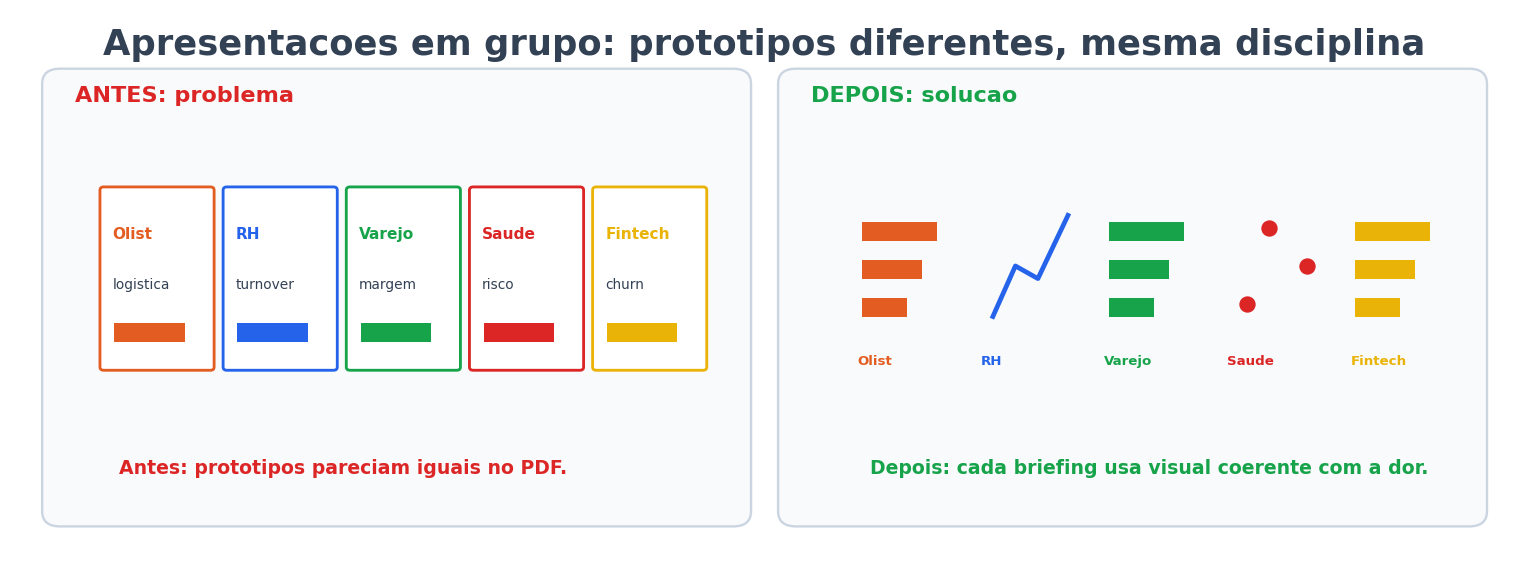
\includegraphics[width=0.62\textwidth]{semana_especial/outputs/cmp_grupos_preview.png}
\end{center}

Os protótipos HTML continuam separados por grupo (\texttt{grupo\_a.html} a \texttt{grupo\_e.html}), mas a figura acima resume a diferença esperada entre eles: cada briefing deve ter visual próprio, coerente com a dor de negócio, e não uma cópia do mesmo layout com dados trocados.
% -------------------------------------------------------

\subsection{Grupo 1 --- E-commerce (Olist)}

\textbf{Dataset:} Brazilian E-Commerce Public Dataset (Olist)\\
\url{https://www.kaggle.com/datasets/olistbr/brazilian-ecommerce}

\textbf{Dor:} atrasos na entrega derrubam as avaliações dos clientes e aumentam o churn de vendedores parceiros da plataforma.

\textbf{Pergunta 1:} ``Em quais estados e categorias os atrasos são mais críticos e qual o impacto nas avaliações (review\_score)?'' \quad \textbf{Pergunta 2:} ``Como o tempo de entrega em dias se correlaciona com a avaliação do cliente?''

\textbf{Big Idea sugerida:} ``Eletrônicos em SP concentram 34\% dos atrasos e puxam o review médio para 3,2 estrelas --- priorizar logística nessa categoria pode elevar o review para 4,1 e reduzir o churn de vendedores em 15\%.'' \quad \textbf{Call to Action:} redesenhar a rota logística de Eletrônicos em SP até Q3/2026.

\textbf{Transformações necessárias:} (1) Join: \texttt{orders $\bowtie$ order\_items $\bowtie$ products $\bowtie$ customers} (chave: \texttt{order\_id} e \texttt{product\_id}). (2) Campo: \texttt{delivery\_delay = order\_delivered\_customer\_date $-$ order\_estimated\_delivery\_date}. (3) Flag: \texttt{is\_late = IF delivery\_delay > 0 THEN ``Atrasado'' ELSE ``No Prazo'' END}. (4) Traduzir categorias com \texttt{product\_category\_name\_translation.csv}. (5) Filtrar status \texttt{canceled} e \texttt{unavailable}.

\textbf{Sheets:} (1) Big Number (\% atrasados por estado/categoria). (2) Mapa coroplético: estado $\times$ \% atraso. (3) Barras horizontais: Top 10 categorias $\times$ \% atraso, líder em laranja. (4) Scatter: dias de atraso $\times$ review\_score + linha de tendência. (5) Linha temporal de atrasos por mês. \textbf{Protótipo HTML:} \texttt{semana\_especial/grupo\_a.html}.

\subsection{Grupo 2 --- People Analytics (IBM HR)}

\textbf{Dataset:} IBM HR Analytics Employee Attrition\\
\url{https://www.kaggle.com/datasets/pavansubhasht/ibm-hr-analytics-attrition-dataset}

\textbf{Dor:} turnover de 28\% em TI custa R\$450k/ano em recrutamento e perda de conhecimento institucional.

\textbf{Pergunta 1:} ``Qual perfil de funcionário tem maior risco de saída e em qual departamento o problema é mais crítico?'' \quad \textbf{Pergunta 2:} ``Satisfação no trabalho e faixa salarial influenciam o turnover?''

\textbf{Big Idea:} ``Funcionários de TI com menos de 2 anos e sem promoção nos últimos 3 anos têm 3$\times$ mais chance de sair --- mentoria focada nesse perfil pode reduzir o turnover de 28\% para 15\% e economizar R\$270k/ano.''

\textbf{Transformações:} (1) \texttt{Attrition\_Num = IF [Attrition]=``Yes'' THEN 1 ELSE 0 END}. (2) \texttt{Turnover\_Rate = AVG(Attrition\_Num) * 100}. (3) Bins de salário (Baixo $<$ 3k / Médio 3k--7k / Alto $>$ 7k). (4) \texttt{Perfil\_Risco = IF [YearsAtCompany] < 2 AND [YearsSinceLastPromotion] > 2 THEN ``Alto Risco'' END}.

\textbf{Sheets:} Big Number (turnover TI vs meta 15\%); barras por departamento com linha de meta; heatmap satisfação $\times$ faixa salarial $\times$ turnover; scatter anos na empresa $\times$ turnover; bullet chart por departamento. \textbf{Protótipo HTML:} \texttt{semana\_especial/grupo\_b.html}.

\subsection{Grupo 3 --- Varejo (Superstore)}

\textbf{Dataset:} Sample Superstore Dataset\\
\url{https://www.kaggle.com/datasets/vivek468/superstore-dataset-final}

\textbf{Dor:} margens negativas em Tecnologia/Sul drenam R\$120k/trimestre do lucro operacional.

\textbf{Pergunta 1:} ``Quais combinações de subcategoria e região geram prejuízo consistente?'' \quad \textbf{Pergunta 2:} ``Existe correlação entre o desconto aplicado e a margem negativa?''

\textbf{Big Idea:} ``Descontos acima de 20\% em Máquinas e Copiadoras na Região Sul concentram 73\% do prejuízo --- capear o desconto em 12\% pode reverter a margem de $-$4,2\% para $+$5,8\%, gerando R\$85k adicionais por trimestre.''

\textbf{Transformações:} (1) \texttt{Margem\_Pct = SUM([Profit]) / SUM([Sales]) * 100}. (2) Bins de desconto (Sem / 0--10\% / 10--20\% / Acima 20\%). (3) \texttt{Prejuizo = IF [Profit] < 0 THEN ``Prejuízo'' ELSE ``Lucro'' END}.

\textbf{Sheets:} Big Number (margem Tech/Sul vs parâmetro de meta 8\%); mapa de calor subcategoria $\times$ região; scatter desconto $\times$ lucro com linhas de referência (0 no eixo Y; 20\% no eixo X); barras agrupadas por região; linha trimestral de margem. \textbf{Protótipo HTML:} \texttt{semana\_especial/grupo\_c.html}.

\subsection{Grupo 4 --- Saúde Pública (Heart Disease)}

\textbf{Dataset:} Heart Disease UCI Dataset\\
\url{https://www.kaggle.com/datasets/johnsmith88/heart-disease-dataset}

\textbf{Dor:} doenças cardíacas = 38\% das internações municipais (custo médio R\$12k/internação).

\textbf{Pergunta 1:} ``Quais fatores de risco têm maior correlação com diagnóstico de doença cardíaca?'' \quad \textbf{Pergunta 2:} ``Qual faixa etária e perfil clínico priorizar em campanhas preventivas?''

\textbf{Big Idea:} ``Colesterol $>$ 240 + pressão arterial $>$ 140 + idade $>$ 55 anos identificam 73\% dos casos de alto risco com apenas 3 variáveis --- triagem preventiva focada nesse perfil pode reduzir internações em 25\% e gerar R\$2,1M de economia anual.''

\textbf{Transformações:} (1) \texttt{Diagnostico = IF [target]=1 THEN ``Doença'' ELSE ``Sem Doença'' END}. (2) \texttt{Sexo = IF [sex]=1 THEN ``Masculino'' ELSE ``Feminino'' END}. (3) Bins de faixa etária ($<$45 / 45--54 / 55--64 / 65+). (4) \texttt{Perfil\_Risco = IF [chol]>240 AND [trestbps]>140 AND [age]>55 THEN ``Alto Risco'' END}. (5) \texttt{Taxa\_Doenca = AVG([target]) * 100}.

\textbf{Sheets:} Big Number (taxa doença em homens $>$ 55); barras de correlação por fator; heatmap faixa etária $\times$ perfil $\times$ taxa; scatter colesterol $\times$ pressão (cor = diagnóstico, linhas em 240 e 140); boxplot de idade por grupo. \textbf{Protótipo HTML:} \texttt{semana\_especial/grupo\_d.html}.

\subsection{Grupo 5 --- Fintech (Credit Card Churn)}

\textbf{Dataset:} Credit Card Customers Dataset\\
\url{https://www.kaggle.com/datasets/sakshigoyal7/credit-card-customers}

\textbf{Dor:} churn de cartão Premium custa R\$2,1M/ano em receita perdida de juros e anuidade.

\textbf{Pergunta 1:} ``Qual perfil de cliente Premium tem maior propensão ao cancelamento?'' \quad \textbf{Pergunta 2:} ``Frequência de uso e limite de crédito influenciam significativamente o churn?''

\textbf{Big Idea:} ``Clientes Premium com limite $<$ R\$10k e menos de 20 transações/ano têm 4$\times$ mais chance de cancelamento --- engajamento proativo focado nesse perfil pode preservar R\$1,2M em receita anual.''

\textbf{Transformações:} (1) \texttt{Churned = IF [Attrition\_Flag]=``Attrited Customer'' THEN 1 ELSE 0 END}. (2) \texttt{Churn\_Rate = AVG(Churned) * 100}. (3) Bins de limite ($<$ R\$10k / R\$10k--30k / $>$ R\$30k). (4) Bins de uso (Baixa $<$ 20 trans / Média 20--50 / Alta $>$ 50). (5) \texttt{Perfil\_Risco = IF [Total\_Trans\_Ct] < 20 AND [Credit\_Limit] < 10000 THEN ``Alto Risco'' END}.

\textbf{Sheets:} Big Number (churn Premium com limite $<$ R\$10k vs benchmark 8\%); barras faixa de limite $\times$ churn; scatter frequência $\times$ valor médio (cor = churn, linha em 20 transações); linha temporal de churn por segmento; heatmap frequência $\times$ limite $\times$ taxa de churn. \textbf{Protótipo HTML:} \texttt{semana\_especial/grupo\_e.html}.

% -------------------------------------------------------
\section{Rubrica de Avaliação --- Apresentação em Grupo}
% -------------------------------------------------------

\begin{tabular}{|p{4.5cm}|r|p{7.5cm}|}
\hline
\textbf{Critério} & \textbf{Peso} & \textbf{Descrição} \\
\hline
Big Idea + Call to Action & 15\% & Explicitada no pitch: ponto de vista + tensão + stake \\
Estrutura do dashboard   & 20\% & Pergunta $\to$ Big Number + Insight IA $\to$ Gráficos $\to$ Tabela \\
Qualidade dos visuais    & 20\% & Títulos-mensagem; cor com propósito; sem chartjunk \\
Insight IA               & 15\% & Acionável; não genérico; ao lado do Big Number \\
Tableau funcional        & 15\% & $\geq$ 1 filtro ou parâmetro funcionando \\
Pitch de 3 minutos       & 15\% & SCR completo; dentro do tempo; call to action explícito \\
\hline
\textbf{Total}           & \textbf{100\%} & \\
\hline
\end{tabular}

% \includegraphics paths são relativos ao diretório de main.tex (aula/)
% =============================================================================

\chapter{Semana Especial (04/05 + 18/05/2026)\\[4pt]Revisão Unidade~II e Dashboard em Grupo}

Este impresso cobre as duas últimas aulas antes das provas. No dia \textbf{04/05} fazemos a revisão de toda a Unidade~II. No dia \textbf{18/05} cada grupo apresenta o dashboard no Tableau --- como está descrito na Parte~III deste documento, que você já recebe hoje para ter duas semanas de preparo. As provas começam na semana de \textbf{25/05}.

% ============================================================
\section*{\Large PARTE I --- REVISÃO DA UNIDADE II (04/05/2026)}
% ============================================================

% -------------------------------------------------------
\section{AED vs.\ Análise Explanatória}
% -------------------------------------------------------

Na Unidade~I vocês exploraram dados para \emph{entender}: histogramas, boxplots, correlações, dados ausentes. A pergunta que guiava cada análise era ``o que os dados me dizem?'' A Unidade~II começa com uma mudança radical de perspectiva. A pergunta agora é outra: \textit{``como eu conto essa história para que alguém tome uma decisão?''}

Quando você sai do papel de analista e entra no papel de comunicador, você faz análise \textbf{explanatória}. A audiência mudou: não é mais você mesmo --- é o CEO, o gerente, o comitê de crédito. Essas pessoas não têm tempo para ver os 200 gráficos que você gerou. Elas precisam de uma mensagem clara suportada pelas evidências certas.

O erro mais comum de analistas iniciantes é mostrar todo o processo exploratório para uma audiência executiva. O resultado: confusão, perda de tempo, e a descoberta mais importante se perde no meio de 30 gráficos. Na análise explanatória, você já sabe a história que vai contar e escolhe \emph{apenas} os gráficos que a sustentam.

\begin{BoardBox}[title=AED vs.\ Explanatória]
\begin{tabular}{@{}lp{4.2cm}p{5.2cm}@{}}
\toprule
 & \textbf{Exploratória (AED)} & \textbf{Explanatória} \\
\midrule
Audiência & O analista & CEO, gerente, investidor \\
Objetivo  & Entender o dado & Provocar uma decisão \\
Linguagem & ``O dado mostra X'' & ``O que este dado muda no que você faz?'' \\
Visuais   & Centenas (maioria descartada) & Só os que servem à mensagem \\
\bottomrule
\end{tabular}
\end{BoardBox}

Toda vez que você estiver construindo uma apresentação, faça esta pergunta para cada gráfico: ``este visual serve à mensagem ou serve à minha curiosidade?'' Se for a segunda opção, ele vai para o apêndice.

\begin{center}
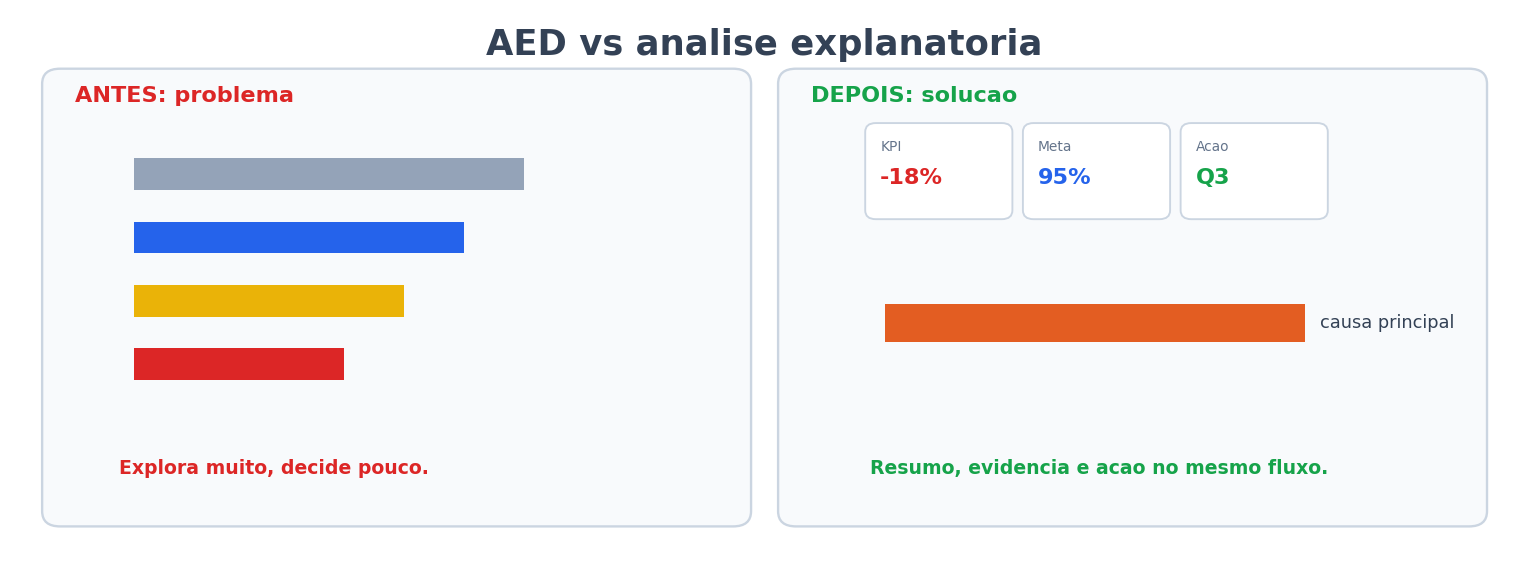
\includegraphics[width=0.58\textwidth]{semana_especial/outputs/cmp_cap2_aed_explanatoria.png}
\end{center}

\textbf{Exemplo prático:} você está analisando dados de alunos em uma instituição de ensino. Na perspectiva exploratória, você gera: correlação entre horas estudadas e nota (0,58), distribuição de notas por sexo, boxplot por disciplina, análise de outliers, falta versus nota. Tudo isso é válido para \emph{você entender} o dado. Mas quando você entra em uma reunião com o diretor e tem 10 minutos, você escolhe apenas \textbf{uma} visualização: alunos com envolvimento familiar baixo + menos de 15 horas de estudo têm nota 9 pontos abaixo da média. Isso é explanatória. A pergunta que o diretor responde depois de ver esse gráfico não é ``que curioso'' --- é ``o que fazemos para resgatar esses alunos?''

% -------------------------------------------------------
\section{Big Idea Framework}
% -------------------------------------------------------

A Big Idea é \textbf{uma única frase} que captura a essência da sua mensagem. Nancy Duarte, em \textit{Datastory} (2019), define que toda boa apresentação de dados deve ter uma Big Idea que a pessoa leva para casa mesmo sem ter visto nenhum gráfico. Ela é o título do seu argumento --- não do seu relatório.

Ela exige três componentes: (1) um \textbf{ponto de vista} --- uma afirmação, não uma observação neutra; (2) a \textbf{tensão} --- o que está em jogo se nada for feito; (3) o \textbf{stake} --- por que a audiência deveria se importar. A fórmula prática é: [recomendação de ação] + [dado concreto que justifica] + [impacto se nada mudar].

\begin{BoardBox}[title=Big Idea --- 3 Componentes e Fórmula]
\begin{enumerate}
  \item \textbf{Ponto de vista:} afirmação, não observação.
  ``O dado mostra X'' \textrightarrow{} não é Big Idea.
  ``Devemos fazer Y porque X'' \textrightarrow{} é Big Idea.
  \item \textbf{Tensão:} o que está em jogo? Risco de não agir?
  \item \textbf{Stake:} por que a audiência deveria se importar?
\end{enumerate}
\smallskip
\textbf{Fórmula:} [ação recomendada] + [dado que justifica] + [impacto financeiro/operacional]
\end{BoardBox}

Veja a diferença: ``A taxa de cancelamento subiu 12\%'' é uma observação --- não orienta nenhuma decisão. ``Se não corrigirmos o onboarding até setembro, perderemos R\$1,2M em receita recorrente nos próximos 12 meses'' tem ponto de vista (corrigir o onboarding), tensão (se não fizermos nada) e stake (R\$1,2M). Essa frase é Big Idea.

O \textbf{teste}: leia para alguém que não viu os dados. Se a resposta for ``interessante'' sem que a pessoa saiba o que fazer --- a Big Idea não está pronta. Ela deve provocar a pergunta ``e como a gente faz isso?''

\begin{center}
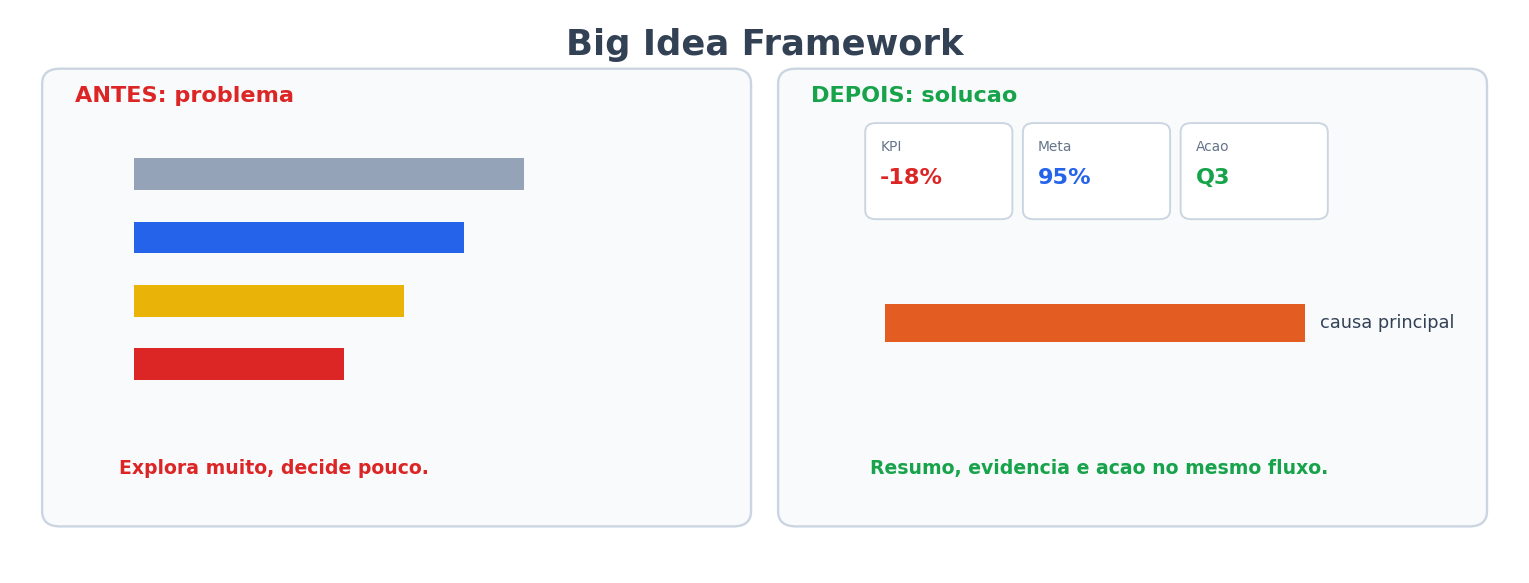
\includegraphics[width=0.58\textwidth]{semana_especial/outputs/cmp_cap2_big_idea.png}
\end{center}

Toda Big Idea está ligada a uma \textbf{pergunta de decisão}: a questão que a audiência precisa responder ao final. Exemplos: ``Devemos expandir para o canal digital ou reforçar o físico?''; ``Qual produto descontinuamos no Q3?''. O analista não precisa ter a resposta --- mas deve apresentar os dados que tornam a resposta possível.

\textbf{Mais exemplos de Big Ideas em diferentes domínios:}
\begin{itemize}
  \item \textit{E-commerce:} ``Frete grátis acima de R\$100 aumenta o ticket médio em 34\%, mas reduz a margem em apenas 8\% --- implementar já seria rentável no Q3.''
  \item \textit{RH:} ``Desenvolvedores sem promoção em 3 anos têm 5$\times$ mais chance de sair; implementar plano de carreira acelerado para 23 talentos preservaria R\$480k em custos de reposição anual.''
  \item \textit{Saúde:} ``Pacientes que recebem chamada de lembrete 24h antes da consulta aumentam a taxa de comparecimento em 41\%; reduz custos operacionais em R\$120k/ano.''
\end{itemize}

\textbf{Teste na prática:} leia sua Big Idea para um colega que não mexe com seus dados. Se ele disser ``muito interessante'', ela ainda não está pronta. Se ele disser ``e quando a gente começa?'', pronto --- você tem uma Big Idea de verdade.

% -------------------------------------------------------
\section{Storyboard e Estrutura Narrativa}
% -------------------------------------------------------

Antes de abrir o Tableau e construir qualquer gráfico, você desenha o \textbf{storyboard} --- um rascunho em papel com os títulos das telas e o tipo de visual em cada uma. Ele força você a pensar na narrativa \emph{antes} de pensar nas ferramentas. Quem abre o Tableau sem storyboard constrói gráficos bonitos sem história.

Nancy Duarte propõe uma estrutura de 4 atos adaptada de narrativas clássicas. O truque é que toda boa apresentação de dados segue exatamente essa ordem: você mostra o estado atual, revela a tensão, apresenta a proposta e termina com um pedido concreto.

\begin{BoardBox}[title=Estrutura Narrativa --- 4 Atos]
\begin{enumerate}
  \item \textbf{Contexto --- O que é:} estado atual; KPIs reais; o ponto de partida.
  \item \textbf{Conflito --- O que poderia ser:} a tensão; o dado que revela o problema.
  \item \textbf{Resolução --- O que proponho:} proposta baseada em evidências.
  \item \textbf{Call to Action:} decisão pedida + responsável + prazo.
\end{enumerate}
\smallskip
\textbf{Em telas:} KPIs atuais \textrightarrow{} problema \textrightarrow{} análise/evidências \textrightarrow{} recomendação
\end{BoardBox}

Cada tela do storyboard deve ter: (1) título que é mensagem --- não ``Gráfico de Barras'', mas sim ``Canal físico custa 4$\times$ mais por venda''; (2) tipo de visual proposto; (3) esboço manual do dado; (4) transição lógica para a próxima tela, como ``por isso, na próxima tela, veja\ldots''

\begin{center}
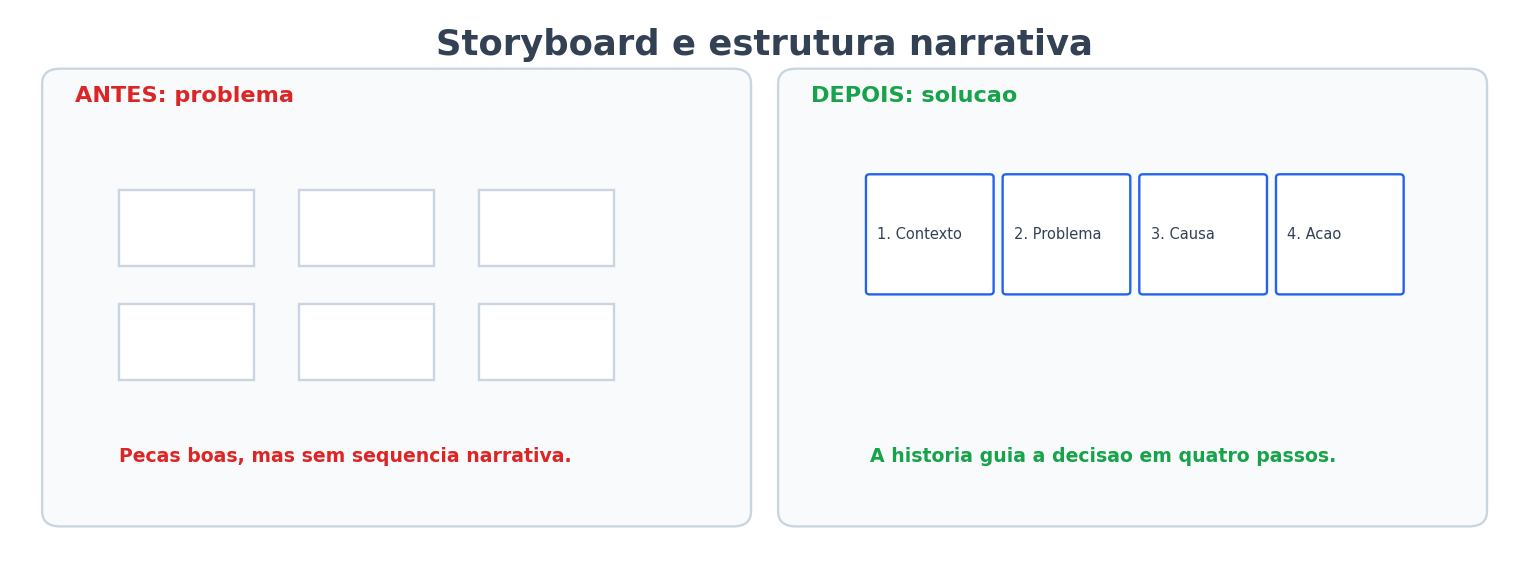
\includegraphics[width=0.58\textwidth]{semana_especial/outputs/cmp_cap2_storyboard.png}
\end{center}

\textbf{Exemplo de storyboard em 4 telas de uma apresentação executiva:}
\begin{enumerate}
  \item \textbf{Tela 1 --- Contexto:} ``Vendas em regiões Sul e Centro-Oeste crescem 15\% acima da média nacional.'' (Big Number destacado + KPI) Transição: ``mas quando olhamos a margem, a história muda radicalmente.''
  \item \textbf{Tela 2 --- Conflito:} ``Essas mesmas regiões têm margem negativa em Tecnologia.'' (Scatter: Desconto vs Margem, cor vermelho no quadrante negativo) Transição: ``achamos 3 subcategorias que concentram 73\% do prejuízo.''
  \item \textbf{Tela 3 --- Análise:} ``Máquinas em SP têm desconto médio de 26\%; Copiadoras em Sul, 23\%; comparando com Nordeste (14\%), o culpado é a política de desconto regional.'' (Tabela + box destacando as 3 categorias críticas) Transição: ``por isso recomendamos\ldots''
  \item \textbf{Tela 4 --- Recomendação:} ``Capar desconto máximo em 12\% em Tecnologia/Sul até 01/junho recupera R\$85k de margem trimestral e move o resultado de -4,2\% para +5,8\%.'' (Simulação com 3 cenários: otimista, realista, pessimista) Próximo passo: ``Gerência Comercial, confirmar a implementação até 15/maio?''
\end{enumerate}

O storyboard em papel \textbf{antes de você abrir o Tableau} economiza semanas de trabalho. Você já sabe qual série temporal é importante, qual drill-down você precisa, quantas telas usará. Quem pula essa etapa muitas vezes constrói um dashboard tecnicamente correto mas narrativamente confuso.

% -------------------------------------------------------
\section{Design de Informação: Pré-atenção e Atributos Visuais}
% -------------------------------------------------------

Antes de você ler deliberadamente qualquer coisa num gráfico, seu cérebro já detectou alguns elementos em menos de 250 milissegundos, sem esforço consciente. Esses são os \textbf{atributos pré-atencionais}. Se você os usa para destacar o que importa, o leitor chega à mensagem antes de ler o título. Se os usa aleatoriamente, o leitor fica desorientado.

A regra de ouro é usar no máximo \textbf{dois atributos pré-atencionais} por visual. Acima disso, a hierarquia colapsa e o olho não sabe onde pousar.

\begin{BoardBox}[title=Atributos Pré-atencionais]
\begin{tabular}{@{}llp{5.2cm}@{}}
\toprule
\textbf{Atributo} & \textbf{Função} & \textbf{Regra de uso} \\
\midrule
Cor        & Destaca, agrupa       & 1 cor de destaque; resto em cinza neutro \\
Tamanho    & Indica magnitude      & Maior = mais importante; consistência obrigatória \\
Posição    & Organiza hierarquia   & Mais importante: canto superior esquerdo \\
Intensidade & Contraste claro/escuro & Mais escuro = mais importante \\
Enclosure  & Agrupa elementos      & Caixa ao redor de dados relacionados \\
\bottomrule
\end{tabular}
\end{BoardBox}

A \textbf{cor} merece atenção especial. Há a cor semântica (vermelho = alerta, verde = ok, amarelo = atenção) e a cor de destaque (uma cor viva para o elemento que carrega a mensagem; todo o resto em cinza). Use cor semântica onde já existe convenção estabelecida. Nunca inverta vermelho e verde sem motivo forte. E lembre: 8\% dos homens têm daltonismo vermelho-verde --- evite que essa combinação seja o único diferenciador.

\begin{center}
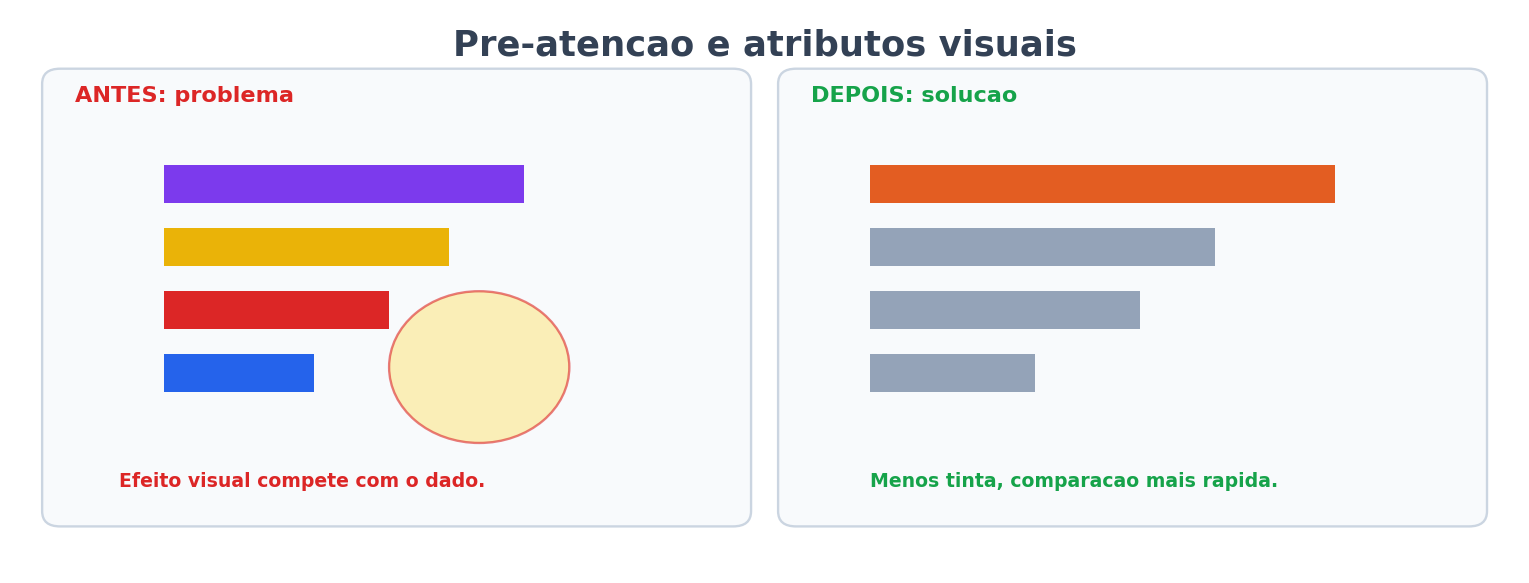
\includegraphics[width=0.58\textwidth]{semana_especial/outputs/cmp_cap2_preatencao.png}
\end{center}

\textbf{Regra de ouro revisitada:} você consegue usar até 2 atributos pré-atencionais em harmonia. Exemplo: na ábaco visual mostrando performance por time, use \textbf{COR} para semântica (verde = meta atingida, vermelho = abaixo) e \textbf{TAMANHO} para magnitude (bolinha grande = time grande, bolinha pequena = time pequeno). Juntos, os dois atributos permitem decodificação instantânea. Se você adicionar um terceiro --- posição espacial não óbvia, ou intensidade de padrão --- o cérebro fica sobrecarregado e falha no teste do relance. Na prática, quando você entra na dúvida de ``será que está confuso?'', sempre está. Remova o terceiro atributo.

% -------------------------------------------------------
\section{Teste do Relance e Título-Mensagem}
% -------------------------------------------------------

O Teste do Relance é simples: mostre o gráfico por 3 segundos, cubra e pergunte à audiência o que viram e qual a mensagem principal. Se não conseguirem responder em 3 segundos, o visual falhou. Não o leitor --- o design.

\begin{BoardBox}[title=Teste do Relance --- Diagnóstico de Falha]
Causas mais comuns de falha:
\begin{itemize}
  \item Título rótulo em vez de título mensagem
  \item Excesso de elementos --- o olho não sabe onde pousar
  \item Cores sem propósito --- todas as barras em cores diferentes
  \item Legenda separada --- o leitor desvia o olhar para decodificar
\end{itemize}
\smallskip
\textbf{Fórmula do título mensagem:} [Sujeito] + [verbo de tendência] + [magnitude]\\
Ex.: ``Churn \textbf{caiu} 34\% após o programa de fidelidade''
\end{BoardBox}

A diferença entre título rótulo e título mensagem é a diferença entre ``Vendas por Região'' e ``Região Sul concentra 58\% das vendas''. O primeiro descreve o que o eixo mostra. O segundo já entrega a informação. Para o executivo com 5 minutos por dia, o título mensagem é o gráfico mais importante --- porque ele consegue ler apenas os títulos e já sabe o que decidir.

\begin{center}
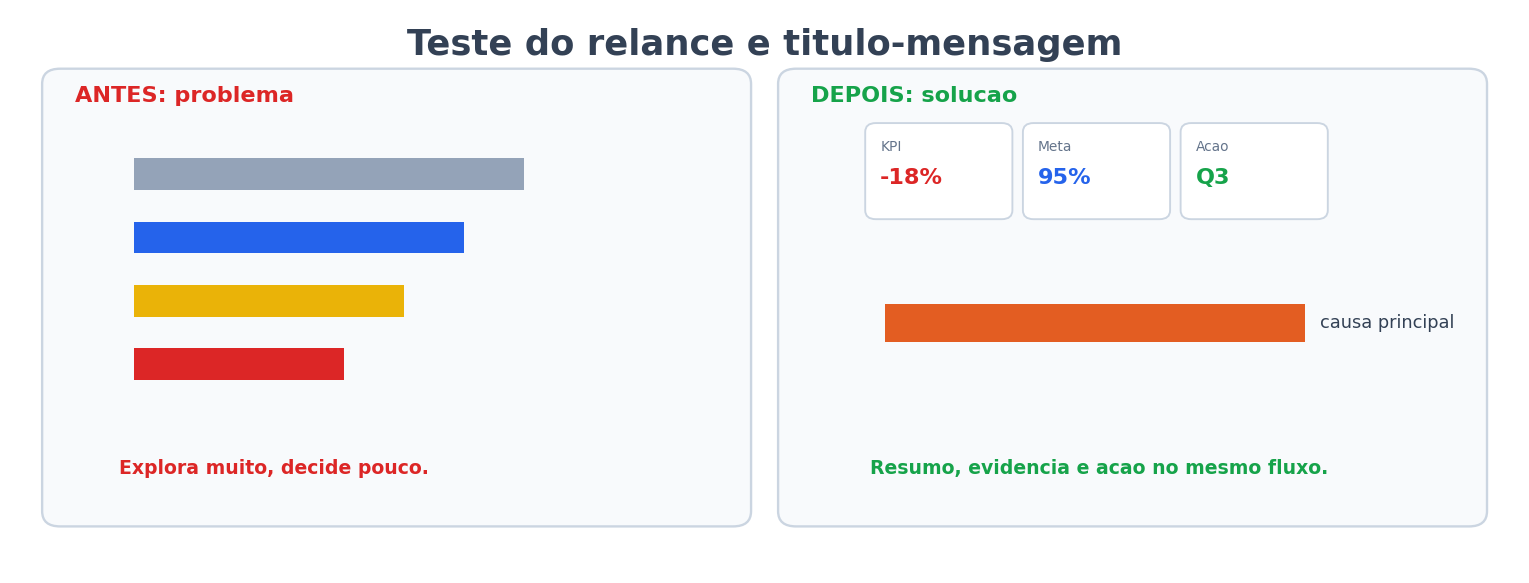
\includegraphics[width=0.58\textwidth]{semana_especial/outputs/cmp_cap2_relance.png}
\end{center}

\textbf{Checklist para passar no Teste do Relance:} (1) título é mensagem, não rótulo? (2) cores comunicam semântica ou prioridade, não decoração? (3) gráfico tem exatamente 1 ou 2 atributos pré-atencionais, não mais? (4) sem ambiguidade: alguém que não viu o dado sabe imediatamente qual a mensagem?

Quando você apresenta um dashboard para alguém pela primeira vez, teste na prática: mostre por 3 segundos, tape a tela e pergunte ``qual a mensagem principal deste gráfico?'' Se a resposta não estiver clara, você ainda tem trabalho. Se estiver absolutamente cristalina --- pronto, passou.

% -------------------------------------------------------
\section{Data-Ink Ratio e Chartjunk}
% -------------------------------------------------------

Edward Tufte (1983) propõe o conceito de \textbf{data-ink ratio}: a proporção da tinta do gráfico que realmente representa dados sobre a tinta total. Maximize esse ratio. Tudo que ocupa tinta sem carregar informação é candidato à remoção.

\begin{BoardBox}[title=Data-Ink Ratio e Chartjunk]
\[
  \text{Data-ink ratio} = \frac{\text{tinta que representa dados}}{\text{tinta total do gráfico}}
\]
\textbf{Chartjunk --- remova:} grades pesadas $\cdot$ barras 3D $\cdot$ sombras $\cdot$ gradientes decorativos $\cdot$ legendas redundantes $\cdot$ ícones temáticos $\cdot$ mais de 3 casas decimais\\[4pt]
\textbf{Princípio:} ``Se eu remover isso, o gráfico fica menos claro?'' Se não --- remova.
\end{BoardBox}

O gráfico de pizza com 8 fatias em 8 cores é o exemplo clássico de chartjunk. O olho humano não compara ângulos com precisão; ele compara comprimentos. Substitua pizza por barras horizontais ordenadas, com 1 cor de destaque para a categoria que carrega a mensagem e rótulos diretos nas barras --- elimine a legenda.

\begin{center}
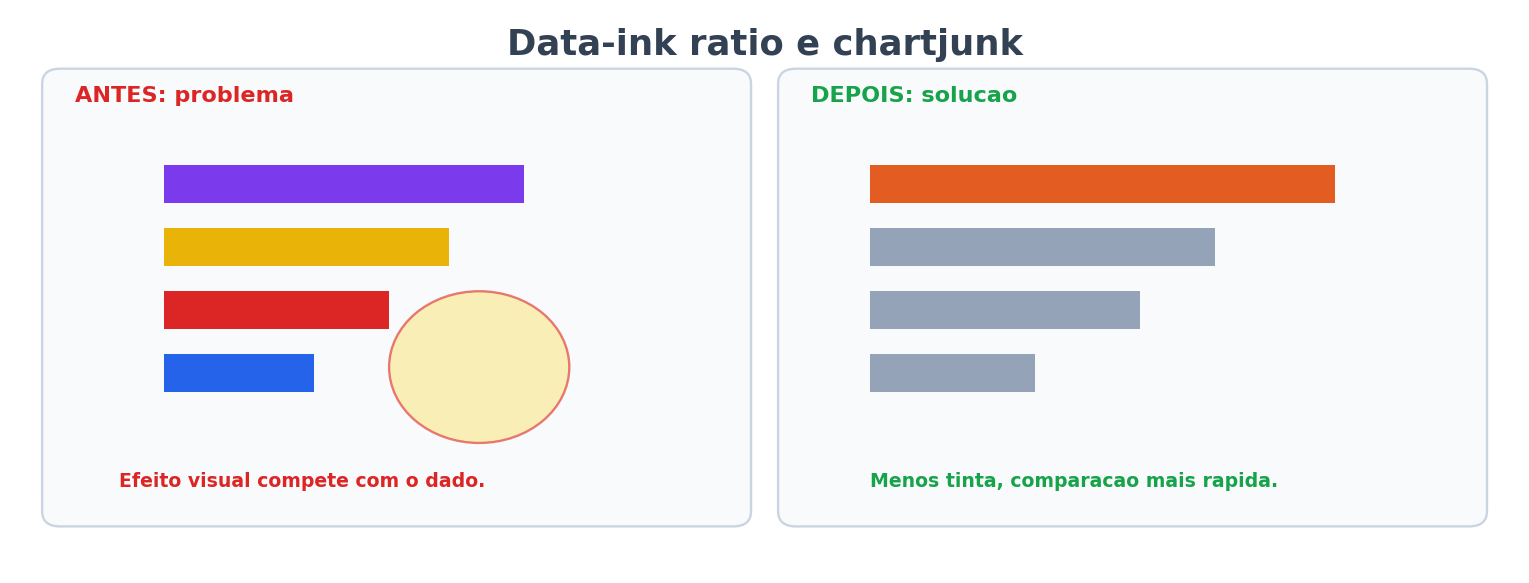
\includegraphics[width=0.58\textwidth]{semana_especial/outputs/cmp_cap2_chartjunk.png}
\end{center}

\textbf{Exemplo de eliminação de chartjunk em 3 passos:} Você tem um gráfico de barras com: (1) grid pesado horizontal e vertical (remove); (2) barras com borda preta (remove); (3) sombra abaixo das barras (remove); (4) legenda no lado dizendo ``Série 1'' (remove --- coloque o rótulo direto na barra); (5) números com 3 casas decimais (reduz para 1 ou 2). Resultado final: data-ink ratio sobe de 50\% para 85\%, o gráfico fica 70\% menor em tamanho visual, e a mensagem fica mais clara.

Em Tableau, a regra é simples: remova toda grid, remova border das marcas, use espaçamento generoso, e ative os rótulos diretos. O resultado é um visual que cabe em uma tela de executivo sem parecer ``deserto''.

% -------------------------------------------------------
\section{Tableau: Filtros, Parâmetros e Ações}
% -------------------------------------------------------

Dois recursos fundamentais de interatividade no Tableau que os alunos frequentemente confundem. A diferença é direta: \textbf{filtros} incluem ou excluem linhas do dataset; \textbf{parâmetros} mudam o cálculo sem filtrar nenhuma linha. Um filtro por estado exibe só os dados de PE --- os dados de SP desaparecem da view. Um parâmetro de métrica permite que o usuário escolha entre Receita ou Margem --- nenhum dado é excluído, apenas o campo calculado muda.

\begin{BoardBox}[title=Filtros vs.\ Parâmetros]
\begin{tabular}{@{}lp{4.5cm}p{5.2cm}@{}}
\toprule
 & \textbf{Filtro} & \textbf{Parâmetro} \\
\midrule
Função   & Inclui/exclui linhas      & Muda o cálculo \\
Uso      & Selecionar região, categoria & Alternar métrica, definir meta, Top N \\
Exemplo  & ``Ver só PE''             & ``Exibir Receita ou Margem?'' \\
\bottomrule
\end{tabular}
\smallskip

\textbf{Campo calculado com parâmetro:}\\
\texttt{IF [Vendas] >= [Meta] THEN ``Atingiu'' ELSE ``Abaixo'' END}
\end{BoardBox}

Sobre a \textbf{hierarquia de filtros}: o Tableau executa filtros em ordem fixa. O mais importante para a prova é o \textbf{Context Filter}. Quando você precisa de Top~N dentro de uma região já filtrada, adicione o filtro de região como Context Filter primeiro --- senão o Tableau calcula o Top~N sobre o dataset inteiro, ignorando o filtro de região.

\begin{center}
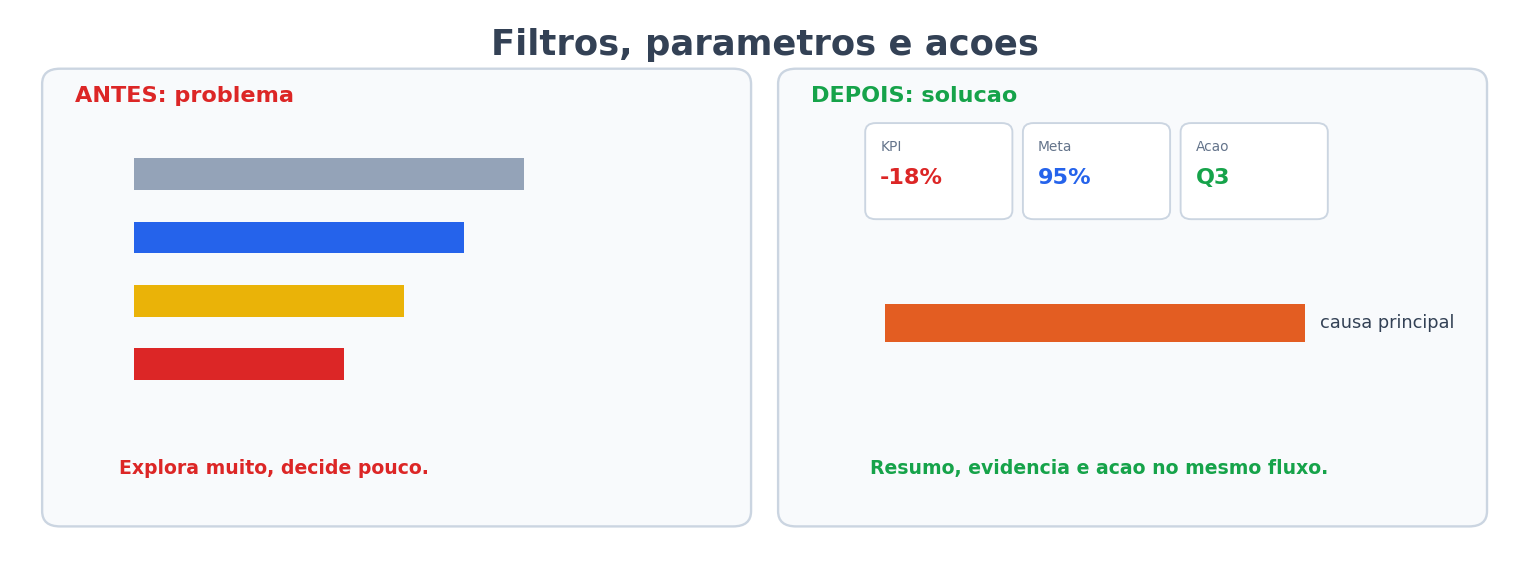
\includegraphics[width=0.58\textwidth]{semana_especial/outputs/cmp_cap2_tableau.png}
\end{center}

\textbf{Pseudocódigo Tableau para parâmetros:} você cria um parâmetro chamado \verb|[Métrica_Selecionada]| com opções ``Receita'', ``Margem'', ``Unidades''. Depois cria um campo calculado:
\begin{quote}\ttfamily
IF [Métrica\_Selecionada] = ``Receita'' THEN [Receita]\\
ELSEIF [Métrica\_Selecionada] = ``Margem'' THEN [Margem]\\
ELSE [Unidades] END
\end{quote}
Quando o usuário muda o parâmetro, o campo calculado avalia instantaneamente e todo o dashboard reflete a mudança. Nenhuma linha é filtrada, apenas o cálculo muda.

\textbf{Context Filter --- quando usar:} você está vendo Top 10 Produtos por Receita em São Paulo. Se você não adicionar ``Estado = SP'' como Context Filter, o Top 10 é calculado sobre TODOS os estados, depois filtrado --- resultado: pode aparecer um produto de outro estado. Com Context Filter, o Top 10 é calculado apenas em SP, garantindo que os 10 maiores de SP apareçam.

\begin{BoardBox}[title=Ações de Dashboard --- 4 Tipos]
\begin{tabular}{@{}lp{4cm}p{4.8cm}@{}}
\toprule
\textbf{Tipo}     & \textbf{O que faz}                  & \textbf{Exemplo} \\
\midrule
Filter action   & Clicar filtra outra view             & Clicar em SP filtra todos os gráficos \\
Highlight       & Destaca sem filtrar                  & Mouse em Região destaca no mapa \\
URL action      & Abre URL com dado selecionado        & Clique abre ficha no ERP \\
Navigate        & Navega entre dashboards              & KPI leva ao painel de drill-down \\
\bottomrule
\end{tabular}
\end{BoardBox}

% -------------------------------------------------------
\section{Dashboards que Forçam Decisão}
% -------------------------------------------------------

Um dashboard pode ser tecnicamente impecável e ainda assim não provocar nenhuma ação. O problema, nesse caso, é de estrutura narrativa. Um dashboard que \textbf{força uma decisão} tem três zonas distintas e em sequência.

\begin{BoardBox}[title=As 3 Zonas do Dashboard Decisório]
\textbf{Zona 1 --- Contexto:} o que está acontecendo agora? KPIs com comparação à meta ou período anterior. Lido em $<$5 segundos. Nenhuma interpretação ainda.

\textbf{Zona 2 --- Diagnóstico:} por que está acontecendo? Drill-down por produto, região, segmento. Permite formular hipóteses --- não confirmar causas.

\textbf{Zona 3 --- Recomendação:} o que fazer? 1--2 recomendações concretas com evidências. Call to Action com \emph{quem}, \emph{o quê} e \emph{até quando}.
\end{BoardBox}

Os \textbf{anti-padrões} mais comuns: (a) tudo sempre verde --- cria conforto falso e impede decisões urgentes; (b) métricas sem definição --- ``Receita'' pode ser bruta, líquida ou MRR, e sem definição explícita cada pessoa lê diferente; (c) 50~KPIs na tela inicial --- granularidade excessiva, o usuário não sabe onde olhar; (d) número isolado sem comparação --- R\$100k de vendas é ótimo ou péssimo em relação ao quê?

\begin{center}
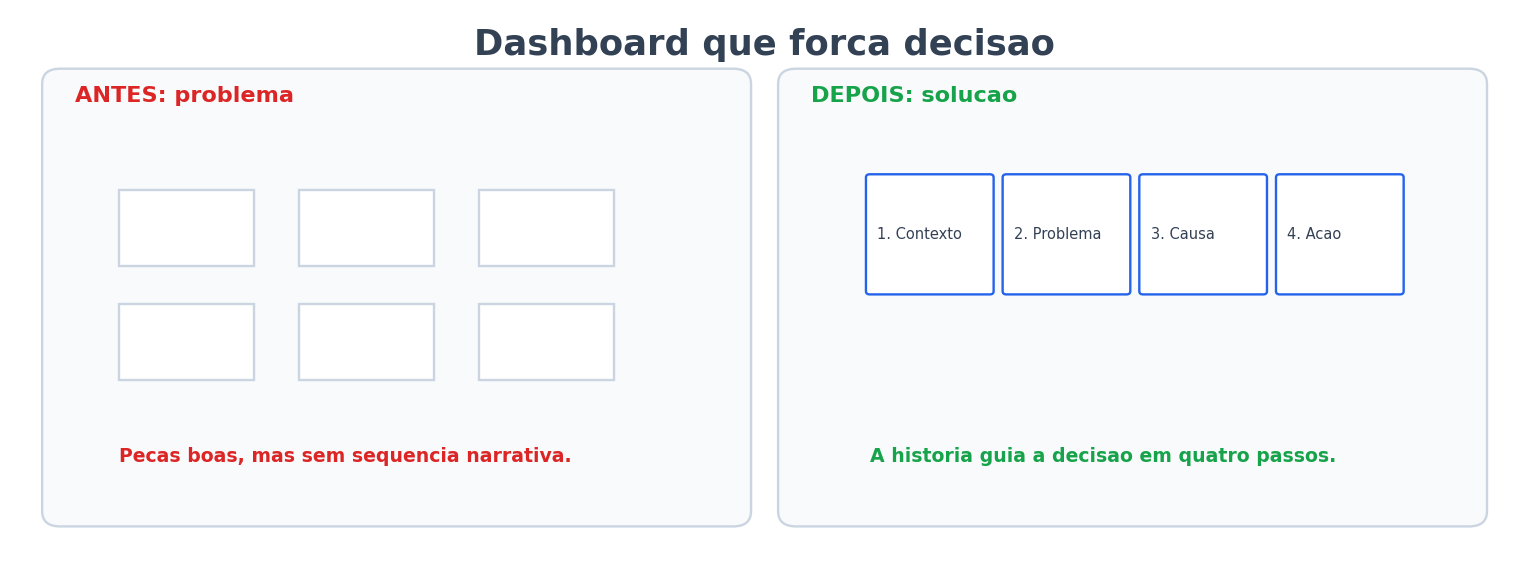
\includegraphics[width=0.58\textwidth]{semana_especial/outputs/cmp_cap2_decisorio.png}
\end{center}

\textbf{Implementação prática das 3 zonas em um dashboard de Vendas:}
\begin{itemize}
  \item \textbf{Zona 1 (Contexto):} 4 KPIs acima da dobra: (1) Receita Mês, Meta, Gap; (2) Margem %; (3) Churn; (4) NPS. Cada KPI mostra ícone de semáforo (verde/amarelo/vermelho). Tempo de leitura: <3 segundos. Nenhuma ação ainda.
  \item \textbf{Zona 2 (Diagnóstico):} 3 gráficos lado a lado: (1) Receita por Região (barras horizontais); (2) Churn vs Desconto (scatter); (3) Série temporal de Margem (linha com meta). Permite que o usuário formule hipóteses (``RJ tem desconto alto demais?'') mas não confirma causas.
  \item \textbf{Zona 3 (Recomendação):} 1 caixa destacada em cor de alerta: ``RJ concentra 65\% da receita mas margem negativa. Reduzir desconto de 26\% para 12\% recupera R\$85k trimestral sem impactar volume (elasticidade = 0,34). Gerência Comercial: implementar até 30/junho.''
\end{itemize}

\textbf{Teste de efetividade:} se seu gerente consegue ler apenas a Zona 3 e já tem uma decisão clara e acionável, sua estrutura funcionou. Se ele precisa voltar para a Zona 2 para entender, significa que a Recomendação não está autossuficiente.

% -------------------------------------------------------
\section{KPIs com Meta, Gap e Tendência}
% -------------------------------------------------------

Um KPI sozinho não decide nada. Para forçar uma decisão, ele precisa de cinco componentes. O número isolado responde ``qual é o valor?'' mas não responde ``isso é bom ou ruim?'' nem ``a situação está melhorando ou piorando?''

\begin{BoardBox}[title=Anatomia de um KPI Decisório]
\begin{enumerate}
  \item \textbf{Valor atual} --- o número real do período
  \item \textbf{Meta (target)} --- o que deveria ser
  \item \textbf{Gap} --- distância em valor absoluto e percentual
  \item \textbf{Tendência} --- seta de alta/baixa ou sparkline
  \item \textbf{Período} --- MTD, YTD, vs ano anterior
\end{enumerate}
\smallskip
\textbf{Bullet chart} (Stephen Few): barra real + barra de meta. Mais informação por cm$^2$ do que qualquer velocímetro ou gauge.
\end{BoardBox}

\begin{center}
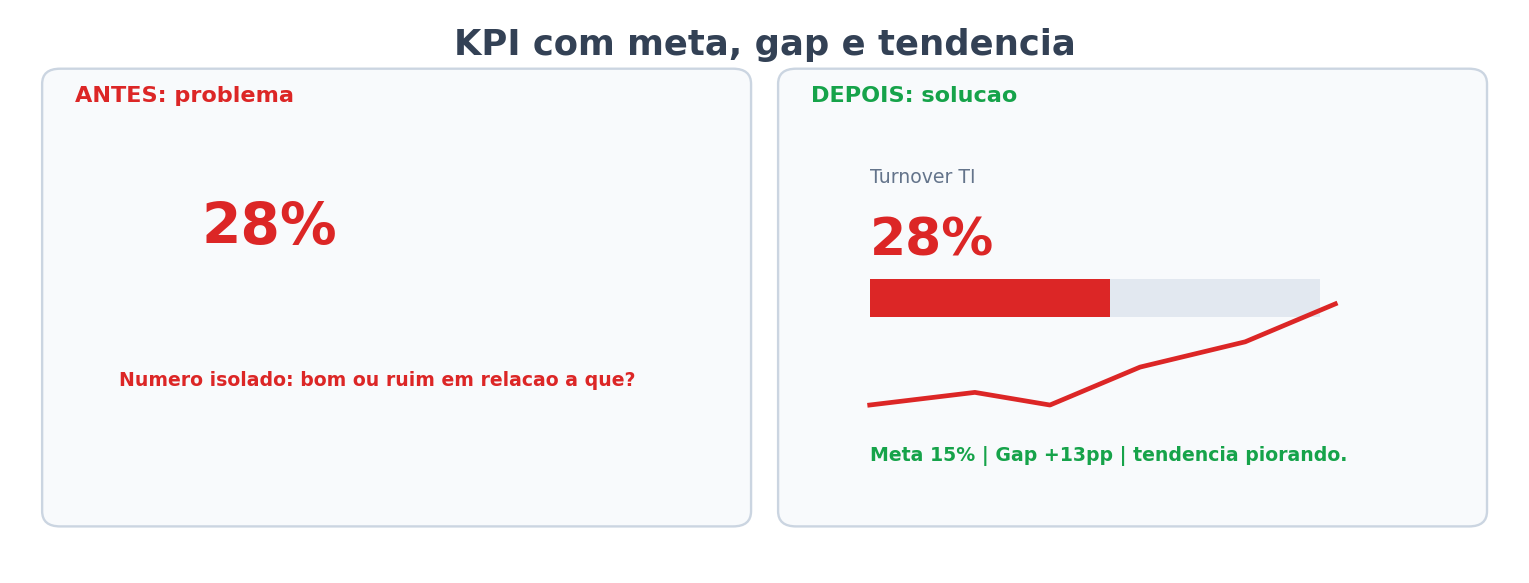
\includegraphics[width=0.58\textwidth]{semana_especial/outputs/cmp_cap2_kpi.png}
\end{center}

\textbf{Exemplos de KPIs bem estruturados em diferentes domínios:}
\begin{itemize}
  \item \textit{E-commerce:} Taxa de Retorno 8\% (Meta: 5\%, Gap: +3pp, Tendência: queda, melhorando, Período: YTD 2026)
  \item \textit{RH:} Turnover TI 28\% (Meta: 15\%, Gap: +13pp, Tendência: alta, piorando, Período: últimos 12 meses)
  \item \textit{Saúde:} Taxa de Readmissão 6,5\% (Meta: 5\%, Gap: +1,5pp, Tendência: alta, piorando, Período: YTD 2026)
\end{itemize}

Quando você tem espaço, a \textbf{bullet chart} (Stephen Few, 2006) é superior ao gauge ou velocímetro porque mostra valor atual, meta, faixa de desempenho bom/médio/ruim, tudo em uma linha horizontal. Se você tiver apenas espaço para um cartão quadrado, use: número grande + meta + gap colorido + sparkline de tendência.

\textbf{Anti-padrão a evitar:} número isolado na tela. Sempre sempre sempre colocar número com: (1) meta ou benchmark; (2) período; (3) tendência. Caso contrário, o número não informa nada --- pode ser bom, ruim, normal. O contexto é o que faz um número virar insight.

% -------------------------------------------------------
\section{Pitch de 3 Minutos}
% -------------------------------------------------------

Três minutos são aproximadamente 450 palavras. Isso é suficiente para convencer alguém --- se e somente se você seguir a estrutura certa. A estrutura SCR (Situação, Complicação, Resolução) tem quatro blocos com tempos definidos.

\begin{BoardBox}[title=Pitch de 3 Minutos --- Estrutura SCR]
\begin{enumerate}
  \item \textbf{Situação (30s):} contexto factual. Comece com o dado impactante, não com introdução genérica.
  \item \textbf{Complicação (45s):} o problema ou oportunidade revelado. Aqui entra a Big Idea.
  \item \textbf{Resolução (60s):} evidência + recomendação com número concreto. Não ``melhorar'' --- sim ``aumentar em 15\%''.
  \item \textbf{Próximo passo (45s):} pedido específico com \textit{verbo + quem + prazo}.
\end{enumerate}
\end{BoardBox}

O erro mais comum: começar com contexto genérico (``vivemos em uma era de dados\ldots'') em vez do dado que mais surpreende. Se você tem 3 minutos e gasta 30 segundos com introdução desnecessária, perdeu 17\% do tempo e a atenção da audiência.

\begin{center}
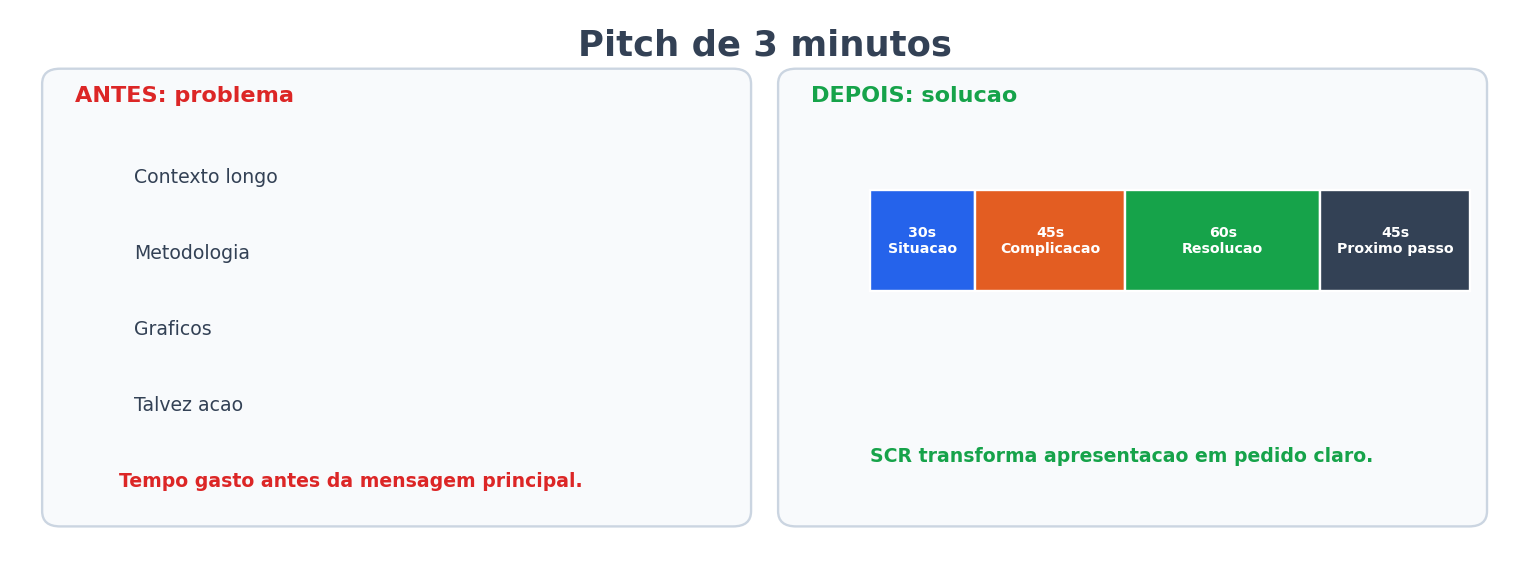
\includegraphics[width=0.58\textwidth]{semana_especial/outputs/cmp_cap2_pitch.png}
\end{center}

\textbf{Exemplo de pitch de 3 minutos em contexto acadêmico:}\\[2pt]
\textbf{Situação (30s):} ``6.607 alunos. 27\% têm nota final menor que 60. Isso significa 1.800 alunos em recuperação, triplicando a carga administrativa e reduzindo a taxa de aprovação final.''\\[2pt]
\textbf{Complicação (45s):} ``Descobrimos que esses alunos compartilham um perfil comum: envolvimento familiar baixo, menos de 15 horas de estudo por semana, e sem ninguém fazendo mentoria. A consequência é uma defasagem de 9 pontos na nota média desse grupo. Se nada mudar, estaremos triplicando esforço e mantendo o mesmo resultado.''\\[2pt]
\textbf{Resolução (60s):} ``Implementamos um programa piloto de mentoria + comunicação familiar com 220 desses alunos em 2025. Resultado: 40\% desse grupo passou a atingir nota acima de 60, aumentando a taxa de aprovação em 8pp e reduzindo custos operacionais de recuperação em R\$45k por ciclo.''\\[2pt]
\textbf{Próximo passo (45s):} ``Recomendo ampliar o programa para todos os alunos em risco (1.800 alunos) no próximo semestre. Implementação começa em julho, com coordenação com coordenação acadêmica. Impacto projetado: +12pp na taxa de aprovação e economia sustentável de R\$120k/ano.''

\textbf{Timing checklist:} você praticou em voz alta? Esse é o teste final. Textos parecem curtos quando lidos mentalmente; no palco, correm 40\% mais rápido do que você pensa. Se você não praticar, vai acabar rápido demais e sobrar tempo, ou vai ficar atropelado tentando terminar em 3 minutos.

% ============================================================
\section*{\Large PARTE II --- QUESTÕES DAS PROVAS --- UNIDADE II}
% ============================================================

As questões abaixo estão no formato exato das provas. \textbf{Prova II Unidade} primeiro (5 questões de 2,0 pts cada). Depois as questões de Unidade~II da \textbf{Prova Final} (Q8, Q9 e Q10 --- 1,0 pt cada). Por fim as questões de Unidade~II da \textbf{Prova II Chamada} (Q8, Q9 e Q10 --- 1,0 pt cada). Os cenários foram levemente adaptados para fins didáticos.

% ============================================================
\subsection*{Prova II Unidade (5 questões $\times$ 2,0 pts)}
% ============================================================

% --- Q1 --- Big Idea
Beatriz é analista de dados em uma rede de 18 farmácias no Recife. Ela foi solicitada a apresentar os resultados de sua análise sobre cancelamentos do programa de fidelidade para a reunião trimestral de diretoria. Após semanas de análise exploratória, Beatriz descobriu que: 72\% dos cancelamentos ocorrem nos primeiros 2 meses; clientes que resgatam pelo menos 1 benefício no primeiro mês têm 80\% de chance de permanecer; o canal de cadastro via WhatsApp tem taxa de retenção 35\% maior que o cadastro em loja; filas no caixa durante o almoço (12h--13h) estão com tempo médio de 8 minutos, gerando reclamações. Beatriz precisa que a diretoria tome uma decisão clara ao final da apresentação.

\begin{SolvedBox}[title=Questão 1 --- Prova II Unidade (2{,}0 pts) --- Big Idea]
Qual alternativa apresenta a \textbf{Big Idea bem formulada} que Beatriz poderia usar?
\begin{enumerate}[label=\Alph*)]
  \item ``Devemos implementar um fluxo de engajamento automático via WhatsApp nos primeiros 2 meses, com nudge para o primeiro resgate, pois isso pode reduzir cancelamentos em até 55\% e aumentar a receita recorrente do programa em R\$220 mil/ano.''
  \item ``Os dados mostram várias informações interessantes sobre o programa de fidelidade.''
  \item ``Analisamos 22.000 registros de clientes do programa entre 2024 e 2025.''
  \item ``A taxa de cancelamento do programa é de 28\% ao ano.''
  \item ``O gráfico de barras mostra a distribuição de cancelamentos por mês.''
\end{enumerate}
\end{SolvedBox}

\textbf{Gabarito: A.} A alternativa A combina os três elementos obrigatórios: (1) ponto de vista --- ``devemos implementar'' é recomendação de ação, não observação passiva; (2) tensão --- 72\% de cancelamentos nos primeiros 2 meses revela a oportunidade desperdiçada; (3) stake financeiro --- R\$220 mil/ano é o argumento decisivo para a diretoria. B é vaga; C é puramente descritiva; D é um número isolado sem orientação; E é rótulo de gráfico sem valor decisório.

\medskip

% --- Q2 --- Design de Dashboard
Rafael é analista de BI em uma rede varejista de eletrodomésticos com 35 lojas. O diretor comercial tem apenas 5 minutos por dia para ver o dashboard. Rafael está decidindo entre duas abordagens de design. \textbf{Opção A:} título ``Vendas Jan/2026: meta superada em 18\% --- foco em Linha Branca''; KPI central ``118\%'' em verde; barras horizontais com a categoria líder destacada em azul escuro; fundo branco, máx.\ 3 cores com propósito, espaço em branco generoso. \textbf{Opção B:} título ``Dashboard Comercial''; 15 gráficos de tipos variados; todas as 8 cores da paleta utilizadas; sem espaço em branco; títulos genéricos ``Gráfico 1'', ``Gráfico 2''.

\begin{SolvedBox}[title=Questão 2 --- Prova II Unidade (2{,}0 pts) --- Design de Dashboard]
Considerando hierarquia visual e Teste do Relance, qual alternativa avalia \textbf{corretamente} as duas opções?
\begin{enumerate}[label=\Alph*)]
  \item A Opção A é superior: título comunica a mensagem com dado concreto, uso restrito de cores direciona a atenção ao que importa, espaço em branco organiza a hierarquia visual, e o dashboard passa no Teste do Relance.
  \item A Opção B é superior porque tem mais gráficos e mais cores, transmitindo mais informação ao diretor.
  \item Ambas são equivalentes em eficácia comunicativa --- o que importa é o dado, não o design.
  \item A Opção A é inferior porque desperdiça espaço que poderia ter mais gráficos.
  \item Títulos como ``Dashboard Comercial'' são mais profissionais e neutros que títulos com dados.
\end{enumerate}
\end{SolvedBox}

\textbf{Gabarito: A.} A Opção A aplica: título-mensagem com dado concreto e relevância imediata; cor de destaque única para guiar o olho; data-ink ratio maximizado sem chartjunk. A Opção B viola todos os princípios: título rótulo que não informa nada; 15 gráficos fragmentam a atenção; 8 cores sem propósito semântico violam o limite atencional; títulos genéricos que não entregam nenhuma mensagem.

\medskip

% --- Q3 --- Filtros e Parâmetros
Marcos é analista de dados em uma rede de 25 concessionárias de veículos no Nordeste. A gerência pediu que o dashboard permitisse: (1) ver apenas as concessionárias de um estado específico; (2) escolher o período de análise entre mês, trimestre ou semestre; (3) alternar a métrica exibida entre Unidades Vendidas e Receita Total. Marcos precisa decidir quais recursos do Tableau usar para cada necessidade.

\begin{SolvedBox}[title=Questão 3 --- Prova II Unidade (2{,}0 pts) --- Tableau: Filtros e Parâmetros]
Qual alternativa apresenta \textbf{corretamente} o recurso do Tableau para cada necessidade?
\begin{enumerate}[label=\Alph*)]
  \item Filtro para selecionar o estado; Parâmetro para o período (campo calculado ajusta a granularidade de datas); Parâmetro para alternar a métrica (\texttt{IF [Métrica]=``Receita'' THEN [Receita] ELSE [Unidades] END}).
  \item Criar 25 dashboards separados, um para cada concessionária, e deixar o gerente escolher qual abrir.
  \item Usar apenas filtros para as 3 necessidades, sem nenhum parâmetro no dashboard.
  \item Exportar os dados para o Excel e calcular os recortes manualmente cada semana.
  \item Usar apenas parâmetros para todas as 3 necessidades, sem nenhum filtro.
\end{enumerate}
\end{SolvedBox}

\textbf{Gabarito: A.} (1) Filtrar por estado é inclusão/exclusão de linhas --- responsabilidade do Quick Filter. (2) Escolher período envolve cálculo de datas dinâmico que só um Parâmetro + campo calculado resolve. (3) Alternar entre Unidades e Receita muda qual campo é calculado, não filtra linhas --- exclusividade do Parâmetro. C está errado porque filtros não trocam campos calculados; E está errado porque parâmetros não excluem linhas do dataset.

\medskip

% --- Q4 --- Dashboard Decisório
Helena é diretora de expansão de uma plataforma de cursos online e precisa apresentar para o board se deve lançar operações presenciais em Caruaru. Ela estruturou o dashboard em 3 seções. \textbf{Seção 1 --- Contexto:} mapa comparando Recife e Caruaru; indicadores de mercado: população-alvo, renda per capita, taxa de adoção de smartphones. \textbf{Seção 2 --- Diagnóstico:} CAC estimado, LTV projetado, taxa de adoção de plataformas similares na região, análise de concorrência local. \textbf{Seção 3 --- Recomendação:} simulação de payback com cenários otimista, realista e pessimista; call-to-action: ``Caruaru --- lançamento Q3/2026, investimento R\$350k, ROI projetado em 18 meses''. O board tomou a decisão em 10 minutos.

\begin{SolvedBox}[title=Questão 4 --- Prova II Unidade (2{,}0 pts) --- Dashboard Decisório]
Qual alternativa explica \textbf{corretamente} por que a estrutura de Helena foi eficaz?
\begin{enumerate}[label=\Alph*)]
  \item O framework Contexto$\to$Diagnóstico$\to$Recomendação funciona porque estabelece o cenário, evidencia a oportunidade e finaliza com ação concreta; os 3 cenários reduzem incerteza; o call-to-action com prazo e ROI torna a decisão acionável.
  \item O dashboard foi eficaz apenas porque tinha gráficos visualmente bonitos e coloridos.
  \item A ordem das 3 seções é irrelevante; qualquer estrutura funcionaria da mesma forma.
  \item Dashboards não devem incluir recomendações; devem apenas mostrar os dados brutos.
  \item O board tomou a decisão rápido porque não leu o dashboard com atenção suficiente.
\end{enumerate}
\end{SolvedBox}

\textbf{Gabarito: A.} A estrutura em 3 zonas replica o processo de decisão humano. O Contexto cria urgência com dados reais sem parecer alarmismo. O Diagnóstico fecha as dúvidas sobre causa raiz (CAC, LTV, adoção). A Recomendação com 3 cenários + ROI + prazo transforma uma apresentação informativa em um dashboard que \emph{força} a decisão. Sem a Zona~3, o board sai da reunião com dados mas sem clareza de ação.

\medskip

% --- Q5 --- Pitch de 3 minutos
Bruno foi selecionado para apresentar sua análise sobre desnutrição infantil no Sertão de Pernambuco em uma competição de dados. Ele tinha apenas 3 minutos. \textbf{Minuto 1 --- Situação:} ``8.200 crianças abaixo de 5 anos apresentam desnutrição moderada ou grave no Agreste/Sertão. Isso representa R\$1,1 bilhão em impacto econômico projetado até 2035. Nossa análise identificou 3 preditores principais.'' \textbf{Minuto 2 --- Complicação:} visual 1 (mapa de calor dos municípios críticos); visual 2 (correlação renda familiar $\times$ índice nutricional); insight: ``crianças em municípios sem CRAS ativo têm 3,5$\times$ mais risco de desnutrição grave''. \textbf{Minuto 3 --- Resolução:} ``Reativar os 12 CRAS desativados pode reduzir a desnutrição em 32\% em 3 anos. Próximo passo: piloto em 3 municípios no 2º semestre com orçamento de R\$480k.'' Bruno termina dentro do tempo e os jurados compreendem claramente a proposta.

\begin{SolvedBox}[title=Questão 5 --- Prova II Unidade (2{,}0 pts) --- Pitch de 3 Minutos]
Qual alternativa descreve \textbf{corretamente} os elementos que tornaram o pitch de Bruno eficaz?
\begin{enumerate}[label=\Alph*)]
  \item O pitch foi eficaz porque: começou com dado impactante (não com contexto genérico); usou apenas 2 visuais estratégicos, sem sobrecarregar; traduziu o insight em ação concreta com métrica de impacto; e terminou com próximo passo com verbo, quantidade e prazo.
  \item O pitch foi eficaz apenas porque durou exatamente 3 minutos, independente do conteúdo.
  \item Bruno deveria ter mostrado todas as visualizações criadas durante a análise exploratória.
  \item Pitches de dados não devem ter gancho emocional; devem começar direto com tabelas de dados.
  \item A recomendação final é desnecessária; os jurados deveriam decidir sozinhos o que fazer com os dados.
\end{enumerate}
\end{SolvedBox}

\textbf{Gabarito: A.} O pitch de Bruno aplica a estrutura SCR com precisão. A Situação começa com dado quantificado (não introdução genérica). A Complicação usa 2 visuais estratégicos (respeita a capacidade atencional) e entrega o insight com magnitude (3,5$\times$). A Resolução tem percentual de impacto (32\%) e o próximo passo tem os 3 elementos de um call-to-action eficaz: verbo (``reativar''), quantidade (12 CRAS / 3 municípios) e prazo (2º semestre).

% ============================================================
\subsection*{Prova Final --- Unidade II (Q8, Q9 e Q10 --- 1,0 pt cada)}
% ============================================================

As questões Q1 a Q7 da Prova Final cobrem Unidade~I (dicionário de dados, qualidade, médias, desvio-padrão, boxplot, dados ausentes e correlação). As três abaixo são as de Unidade~II.

% --- Final Q8
\begin{SolvedBox}[title=Questão 8 (Prova Final) --- Big Idea (1{,}0 pt)]
Qual frase representa uma \textbf{Big Idea bem formulada} para uma apresentação à diretoria?
\begin{enumerate}[label=\Alph*)]
  \item ``Devemos implantar bônus de permanência nos 2 primeiros anos de empresa, pois a análise mostra redução de 40\% no turnover e economia de R\$180k em custos de reposição de pessoal.''
  \item ``O gráfico de linhas mostra a evolução do turnover por trimestre.''
  \item ``Analisamos 10.000 registros de colaboradores no período de 2023 a 2025.''
  \item ``Os dados de recursos humanos são interessantes e apresentam padrões relevantes.''
  \item ``Tabela 1: distribuição de turnover por departamento e nível hierárquico.''
\end{enumerate}
\end{SolvedBox}

\textbf{Gabarito: A.} A alternativa A tem ponto de vista (``devemos implantar''), tensão (turnover elevado gerando custo de reposição) e stake financeiro concreto (R\$180k). As demais são rótulos de visual (B, E), descrições genéricas (C) ou afirmações sem orientação de ação (D).

% --- Final Q9
\begin{SolvedBox}[title=Questão 9 (Prova Final) --- Design de Dashboard (1{,}0 pt)]
Qual prática é \textbf{recomendada} para criar um dashboard executivo eficaz?
\begin{enumerate}[label=\Alph*)]
  \item Títulos que comunicam a mensagem com dado concreto, uso máximo de 3 cores com propósito semântico, e espaço em branco para organizar a hierarquia visual.
  \item Usar todas as cores disponíveis na paleta para tornar o dashboard visualmente mais atrativo.
  \item Colocar o máximo de gráficos possível para demonstrar todo o trabalho analítico realizado.
  \item Eliminar completamente o espaço em branco para aproveitar toda a área disponível na tela.
  \item Usar títulos genéricos como ``Gráfico 1'' para não influenciar a interpretação do leitor.
\end{enumerate}
\end{SolvedBox}

\textbf{Gabarito: A.} Os princípios de design estabelecem: (a) título-mensagem entrega a informação antes de qualquer leitura do gráfico; (b) máx.\ 3 cores com propósito semântico respeita o limite atencional (mais de 6 cores e o leitor perde a associação cor-categoria); (c) espaço em branco não é desperdício --- é o organizador silencioso da hierarquia visual (leitura em Z).

% --- Final Q10
\begin{SolvedBox}[title=Questão 10 (Prova Final) --- Tableau: Filtros e Parâmetros (1{,}0 pt)]
No Tableau, qual recurso permite que o usuário ajuste \textbf{dinamicamente} uma meta de vendas e o dashboard atualize automaticamente a comparação de desempenho de cada região?
\begin{enumerate}[label=\Alph*)]
  \item Parâmetro combinado com campo calculado que usa o valor do parâmetro como referência.
  \item Exportar o relatório para PDF e recalcular os comparativos manualmente.
  \item Imprimir o dashboard e atualizar os números com caneta a cada nova meta.
  \item Copiar os dados para o Excel e usar PROCV para comparar com a meta.
  \item Usar apenas gráficos estáticos com os dados fixos do período selecionado.
\end{enumerate}
\end{SolvedBox}

\textbf{Gabarito: A.} O parâmetro é um valor dinâmico controlado pelo usuário que pode ser referenciado em qualquer campo calculado. No campo \texttt{IF SUM([Vendas]) >= [Meta] THEN ``Atingiu'' ELSE ``Abaixo'' END}, o usuário ajusta a meta em tempo real e o indicador atualiza instantaneamente. O filtro não faz isso porque inclui/exclui linhas, não altera cálculos.

% ============================================================
\subsection*{Prova II Chamada --- Unidade II (Q8, Q9 e Q10 --- 1,0 pt cada)}
% ============================================================

A Prova II Chamada cobre todo o semestre. As questões Q1 a Q7 são de Unidade~I. As três abaixo são as de Unidade~II.

% --- II Chamada Q8
Uma analista de microcrédito rural trabalha com 30.000 contratos de agricultores no Sertão de PE. Ela identificou: inadimplência geral de 14\% ao ano; clientes sem visita de agente nos últimos 60 dias têm 38\% de inadimplência; clientes com histórico de microcrédito renovado têm apenas 6\% de inadimplência; custo de captação de novo cliente: R\$380.

\begin{SolvedBox}[title=Questão 8 (Prova II Chamada) --- Big Idea (1{,}0 pt)]
Qual alternativa representa a \textbf{melhor Big Idea} para apresentar ao comitê de crédito?
\begin{enumerate}[label=\Alph*)]
  \item ``Devemos implantar visita de agente a cada 45 dias para clientes sem contato recente, pois isso pode reduzir a inadimplência de 38\% para aproximadamente 6\%, economizando R\$210 mil/ano em perdas e evitando R\$380 por cliente em custos de reposição.''
  \item ``A inadimplência do portfólio é de 14\% ao ano.''
  \item ``Analisamos 30.000 contratos de microcrédito ao longo de 18 meses de operação.''
  \item ``Clientes inadimplentes existem por vários motivos e o cenário é complexo.''
  \item ``O gráfico de linhas mostra a tendência de inadimplência nos últimos 24 meses.''
\end{enumerate}
\end{SolvedBox}

\textbf{Gabarito: A.} Mesma lógica: ponto de vista (``devemos implantar'') + dado concreto que cria urgência (38\% vs 6\%) + impacto financeiro quantificado (R\$210k + R\$380/cliente). As demais são vagas, descritivas ou apenas números sem orientação de ação.

% --- II Chamada Q9
\begin{SolvedBox}[title=Questão 9 (Prova II Chamada) --- Título-Mensagem e Teste do Relance (1{,}0 pt)]
Um dashboard executivo precisa mostrar se a meta de vendas foi atingida no trimestre. Qual título de gráfico é \textbf{mais eficaz} segundo o princípio do Teste do Relance?
\begin{enumerate}[label=\Alph*)]
  \item ``Meta superada: Vendas de R\$2,3M excedem a meta de R\$2,0M em 15\%''
  \item ``Dashboard de Vendas Q4''
  \item ``Gráfico 1: Desempenho Comercial''
  \item ``Análise Trimestral de Resultados''
  \item ``Dados de Performance do Período''
\end{enumerate}
\end{SolvedBox}

\textbf{Gabarito: A.} A alternativa A é o único título-mensagem: traz o sujeito (vendas), o verbo de resultado (``superada''), a magnitude (R\$2,3M vs R\$2,0M) e o delta percentual (15\%). Em 3 segundos de relance, o leitor já sabe o resultado sem precisar ler o gráfico. As demais alternativas são todos títulos rótulo: descrevem o tipo ou o período do gráfico, mas não entregam nenhuma informação.

% --- II Chamada Q10
\begin{SolvedBox}[title=Questão 10 (Prova II Chamada) --- Tableau: Ação de Filtro (1{,}0 pt)]
Um analista construiu um dashboard no Tableau. Ele quer que ao clicar em uma barra de um gráfico de vendas por região, um segundo gráfico no mesmo dashboard mostre automaticamente os detalhes daquela região. Qual recurso do Tableau realiza isso?
\begin{enumerate}[label=\Alph*)]
  \item Ação de Filtro (Filter Action): uma seleção em uma visualização filtra outra visualização do mesmo dashboard.
  \item Exportar o dashboard para PDF e criar versões separadas por região manualmente.
  \item Criar 10 dashboards diferentes, um para cada região, e publicar todos no Tableau Public.
  \item Usar apenas parâmetros sem configurar nenhuma ação de dashboard.
  \item Formatação condicional de células no estilo planilha.
\end{enumerate}
\end{SolvedBox}

\textbf{Gabarito: A.} A Filter Action é exatamente o mecanismo de interatividade entre sheets em um dashboard Tableau. Ao configurar: Source Sheet (gráfico de regiões) $\to$ Target Sheet (gráfico de detalhe) $\to$ Trigger: Select, o clique em qualquer barra regional passa o valor selecionado como filtro para a view de destino, atualizando-a instantaneamente. É o recurso mais usado em drill-down de dashboards.

% ============================================================
\section*{\Large PARTE III --- APRESENTAÇÃO EM GRUPO (18/05/2026)}
% ============================================================

% -------------------------------------------------------
\section{Dinâmica, Regras e Estrutura}
% -------------------------------------------------------

Na aula de 18 de maio cada grupo apresenta seu dashboard construído no Tableau durante a própria aula. Este material foi entregue em 04/05 para que cada grupo tenha 14 dias de preparo. O link do Tableau Public deve ser enviado no chat antes de a apresentação começar --- o professor testa ao vivo. O tempo de apresentação é 3 minutos de pitch + 2 minutos de perguntas da turma.

A estrutura obrigatória do dashboard é: \textbf{Pergunta de negócio} $\to$ \textbf{Big Number} (coluna esquerda) + \textbf{Insight gerado por IA} (coluna direita) $\to$ \textbf{Gráficos que respondem à pergunta} $\to$ \textbf{Próxima pergunta} $\to$ \textbf{Gráficos} $\to$ \textbf{Tabela analítica final} (largura total). O Call to Action aparece como título do dashboard ou painel de texto no rodapé.

\begin{BoardBox}[title=Boas Práticas Obrigatórias no Dashboard]
\begin{enumerate}
  \item \textbf{Cor com propósito:} 1 cor de destaque; resto em cinza. Sem arco-íris.
  \item \textbf{Título-mensagem em cada gráfico:} não ``Gráfico de Barras'' --- sim ``X lidera com 2,4$\times$ mais que a média''.
  \item \textbf{Big Number:} fonte $\geq$ 24pt, rótulo descritivo abaixo, indicador de gap com direção + delta.
  \item \textbf{Insight IA:} painel de texto ao lado do Big Number, entre aspas, com rótulo \textbf{[Insight IA]}.
  \item \textbf{Tabela analítica final:} dados consolidados para quem quiser o detalhe.
  \item \textbf{$\geq$ 1 filtro ou parâmetro} funcionando --- dashboard não pode ser puramente estático.
\end{enumerate}
\end{BoardBox}

Enquanto um grupo apresenta, os demais anotam em papel: (1) Big Idea em 1 frase do que ouviram; (2) uma decisão que tomariam com base no dashboard; (3) uma sugestão de melhoria. Isso exercita escuta ativa e gera feedback de valor para o apresentador.

\begin{BoardBox}[title=Prompt para Gerar o Insight IA (ChatGPT ou Gemini)]
\begin{quote}
\small\textit{``Você é analista de dados sênior especializado em [ÁREA DO NEGÓCIO]. Com base nos dados abaixo, gere UM insight acionável em até 3 linhas: (1) padrão não óbvio, (2) impacto quantificado com número concreto, (3) ação específica com estimativa de resultado. Contexto do negócio: [DOR DO GRUPO EM 1 FRASE]. Dados: [COLE O RESUMO DA TABELA ANALÍTICA]. Formato: 1 frase entre aspas, iniciando com o dado mais impactante.''}
\end{quote}
\end{BoardBox}

% -------------------------------------------------------
\section{Grupos e Briefings}

\begin{center}
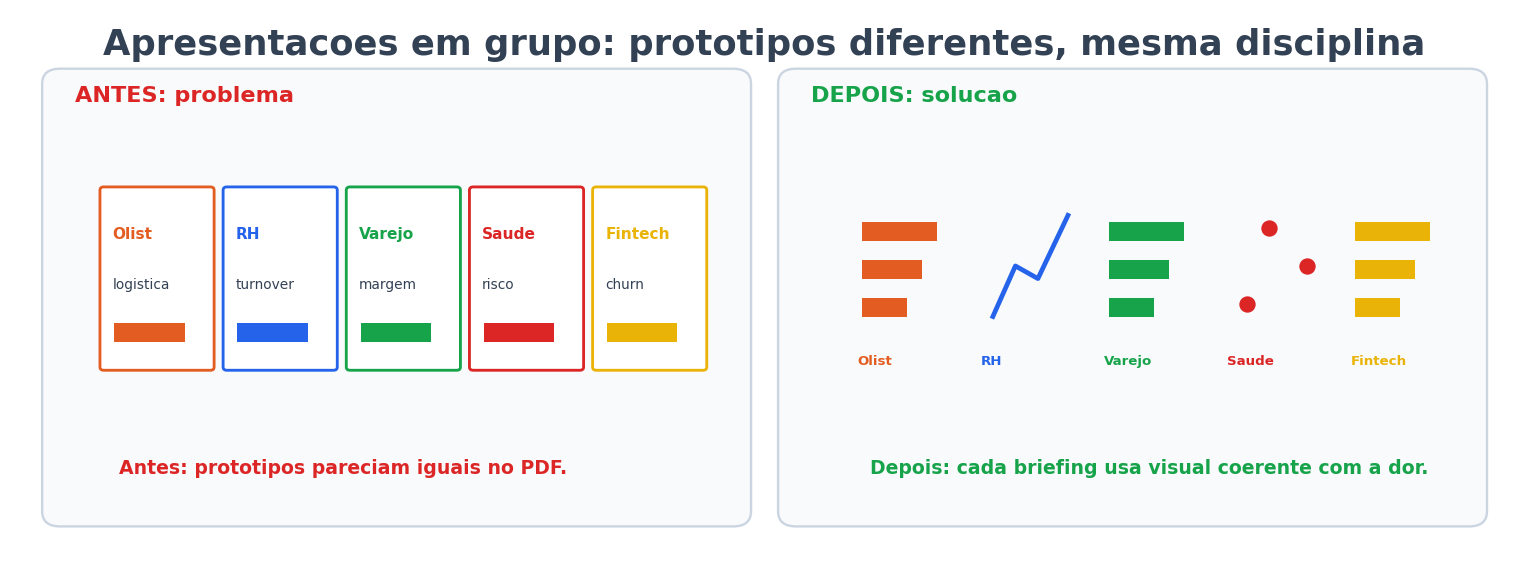
\includegraphics[width=0.62\textwidth]{semana_especial/outputs/cmp_grupos_preview.png}
\end{center}

Os protótipos HTML continuam separados por grupo (\texttt{grupo\_a.html} a \texttt{grupo\_e.html}), mas a figura acima resume a diferença esperada entre eles: cada briefing deve ter visual próprio, coerente com a dor de negócio, e não uma cópia do mesmo layout com dados trocados.
% -------------------------------------------------------

\subsection{Grupo 1 --- E-commerce (Olist)}

\textbf{Dataset:} Brazilian E-Commerce Public Dataset (Olist)\\
\url{https://www.kaggle.com/datasets/olistbr/brazilian-ecommerce}

\textbf{Dor:} atrasos na entrega derrubam as avaliações dos clientes e aumentam o churn de vendedores parceiros da plataforma.

\textbf{Pergunta 1:} ``Em quais estados e categorias os atrasos são mais críticos e qual o impacto nas avaliações (review\_score)?'' \quad \textbf{Pergunta 2:} ``Como o tempo de entrega em dias se correlaciona com a avaliação do cliente?''

\textbf{Big Idea sugerida:} ``Eletrônicos em SP concentram 34\% dos atrasos e puxam o review médio para 3,2 estrelas --- priorizar logística nessa categoria pode elevar o review para 4,1 e reduzir o churn de vendedores em 15\%.'' \quad \textbf{Call to Action:} redesenhar a rota logística de Eletrônicos em SP até Q3/2026.

\textbf{Transformações necessárias:} (1) Join: \texttt{orders $\bowtie$ order\_items $\bowtie$ products $\bowtie$ customers} (chave: \texttt{order\_id} e \texttt{product\_id}). (2) Campo: \texttt{delivery\_delay = order\_delivered\_customer\_date $-$ order\_estimated\_delivery\_date}. (3) Flag: \texttt{is\_late = IF delivery\_delay > 0 THEN ``Atrasado'' ELSE ``No Prazo'' END}. (4) Traduzir categorias com \texttt{product\_category\_name\_translation.csv}. (5) Filtrar status \texttt{canceled} e \texttt{unavailable}.

\textbf{Sheets:} (1) Big Number (\% atrasados por estado/categoria). (2) Mapa coroplético: estado $\times$ \% atraso. (3) Barras horizontais: Top 10 categorias $\times$ \% atraso, líder em laranja. (4) Scatter: dias de atraso $\times$ review\_score + linha de tendência. (5) Linha temporal de atrasos por mês. \textbf{Protótipo HTML:} \texttt{semana\_especial/grupo\_a.html}.

\subsection{Grupo 2 --- People Analytics (IBM HR)}

\textbf{Dataset:} IBM HR Analytics Employee Attrition\\
\url{https://www.kaggle.com/datasets/pavansubhasht/ibm-hr-analytics-attrition-dataset}

\textbf{Dor:} turnover de 28\% em TI custa R\$450k/ano em recrutamento e perda de conhecimento institucional.

\textbf{Pergunta 1:} ``Qual perfil de funcionário tem maior risco de saída e em qual departamento o problema é mais crítico?'' \quad \textbf{Pergunta 2:} ``Satisfação no trabalho e faixa salarial influenciam o turnover?''

\textbf{Big Idea:} ``Funcionários de TI com menos de 2 anos e sem promoção nos últimos 3 anos têm 3$\times$ mais chance de sair --- mentoria focada nesse perfil pode reduzir o turnover de 28\% para 15\% e economizar R\$270k/ano.''

\textbf{Transformações:} (1) \texttt{Attrition\_Num = IF [Attrition]=``Yes'' THEN 1 ELSE 0 END}. (2) \texttt{Turnover\_Rate = AVG(Attrition\_Num) * 100}. (3) Bins de salário (Baixo $<$ 3k / Médio 3k--7k / Alto $>$ 7k). (4) \texttt{Perfil\_Risco = IF [YearsAtCompany] < 2 AND [YearsSinceLastPromotion] > 2 THEN ``Alto Risco'' END}.

\textbf{Sheets:} Big Number (turnover TI vs meta 15\%); barras por departamento com linha de meta; heatmap satisfação $\times$ faixa salarial $\times$ turnover; scatter anos na empresa $\times$ turnover; bullet chart por departamento. \textbf{Protótipo HTML:} \texttt{semana\_especial/grupo\_b.html}.

\subsection{Grupo 3 --- Varejo (Superstore)}

\textbf{Dataset:} Sample Superstore Dataset\\
\url{https://www.kaggle.com/datasets/vivek468/superstore-dataset-final}

\textbf{Dor:} margens negativas em Tecnologia/Sul drenam R\$120k/trimestre do lucro operacional.

\textbf{Pergunta 1:} ``Quais combinações de subcategoria e região geram prejuízo consistente?'' \quad \textbf{Pergunta 2:} ``Existe correlação entre o desconto aplicado e a margem negativa?''

\textbf{Big Idea:} ``Descontos acima de 20\% em Máquinas e Copiadoras na Região Sul concentram 73\% do prejuízo --- capear o desconto em 12\% pode reverter a margem de $-$4,2\% para $+$5,8\%, gerando R\$85k adicionais por trimestre.''

\textbf{Transformações:} (1) \texttt{Margem\_Pct = SUM([Profit]) / SUM([Sales]) * 100}. (2) Bins de desconto (Sem / 0--10\% / 10--20\% / Acima 20\%). (3) \texttt{Prejuizo = IF [Profit] < 0 THEN ``Prejuízo'' ELSE ``Lucro'' END}.

\textbf{Sheets:} Big Number (margem Tech/Sul vs parâmetro de meta 8\%); mapa de calor subcategoria $\times$ região; scatter desconto $\times$ lucro com linhas de referência (0 no eixo Y; 20\% no eixo X); barras agrupadas por região; linha trimestral de margem. \textbf{Protótipo HTML:} \texttt{semana\_especial/grupo\_c.html}.

\subsection{Grupo 4 --- Saúde Pública (Heart Disease)}

\textbf{Dataset:} Heart Disease UCI Dataset\\
\url{https://www.kaggle.com/datasets/johnsmith88/heart-disease-dataset}

\textbf{Dor:} doenças cardíacas = 38\% das internações municipais (custo médio R\$12k/internação).

\textbf{Pergunta 1:} ``Quais fatores de risco têm maior correlação com diagnóstico de doença cardíaca?'' \quad \textbf{Pergunta 2:} ``Qual faixa etária e perfil clínico priorizar em campanhas preventivas?''

\textbf{Big Idea:} ``Colesterol $>$ 240 + pressão arterial $>$ 140 + idade $>$ 55 anos identificam 73\% dos casos de alto risco com apenas 3 variáveis --- triagem preventiva focada nesse perfil pode reduzir internações em 25\% e gerar R\$2,1M de economia anual.''

\textbf{Transformações:} (1) \texttt{Diagnostico = IF [target]=1 THEN ``Doença'' ELSE ``Sem Doença'' END}. (2) \texttt{Sexo = IF [sex]=1 THEN ``Masculino'' ELSE ``Feminino'' END}. (3) Bins de faixa etária ($<$45 / 45--54 / 55--64 / 65+). (4) \texttt{Perfil\_Risco = IF [chol]>240 AND [trestbps]>140 AND [age]>55 THEN ``Alto Risco'' END}. (5) \texttt{Taxa\_Doenca = AVG([target]) * 100}.

\textbf{Sheets:} Big Number (taxa doença em homens $>$ 55); barras de correlação por fator; heatmap faixa etária $\times$ perfil $\times$ taxa; scatter colesterol $\times$ pressão (cor = diagnóstico, linhas em 240 e 140); boxplot de idade por grupo. \textbf{Protótipo HTML:} \texttt{semana\_especial/grupo\_d.html}.

\subsection{Grupo 5 --- Fintech (Credit Card Churn)}

\textbf{Dataset:} Credit Card Customers Dataset\\
\url{https://www.kaggle.com/datasets/sakshigoyal7/credit-card-customers}

\textbf{Dor:} churn de cartão Premium custa R\$2,1M/ano em receita perdida de juros e anuidade.

\textbf{Pergunta 1:} ``Qual perfil de cliente Premium tem maior propensão ao cancelamento?'' \quad \textbf{Pergunta 2:} ``Frequência de uso e limite de crédito influenciam significativamente o churn?''

\textbf{Big Idea:} ``Clientes Premium com limite $<$ R\$10k e menos de 20 transações/ano têm 4$\times$ mais chance de cancelamento --- engajamento proativo focado nesse perfil pode preservar R\$1,2M em receita anual.''

\textbf{Transformações:} (1) \texttt{Churned = IF [Attrition\_Flag]=``Attrited Customer'' THEN 1 ELSE 0 END}. (2) \texttt{Churn\_Rate = AVG(Churned) * 100}. (3) Bins de limite ($<$ R\$10k / R\$10k--30k / $>$ R\$30k). (4) Bins de uso (Baixa $<$ 20 trans / Média 20--50 / Alta $>$ 50). (5) \texttt{Perfil\_Risco = IF [Total\_Trans\_Ct] < 20 AND [Credit\_Limit] < 10000 THEN ``Alto Risco'' END}.

\textbf{Sheets:} Big Number (churn Premium com limite $<$ R\$10k vs benchmark 8\%); barras faixa de limite $\times$ churn; scatter frequência $\times$ valor médio (cor = churn, linha em 20 transações); linha temporal de churn por segmento; heatmap frequência $\times$ limite $\times$ taxa de churn. \textbf{Protótipo HTML:} \texttt{semana\_especial/grupo\_e.html}.

% -------------------------------------------------------
\section{Rubrica de Avaliação --- Apresentação em Grupo}
% -------------------------------------------------------

\begin{tabular}{|p{4.5cm}|r|p{7.5cm}|}
\hline
\textbf{Critério} & \textbf{Peso} & \textbf{Descrição} \\
\hline
Big Idea + Call to Action & 15\% & Explicitada no pitch: ponto de vista + tensão + stake \\
Estrutura do dashboard   & 20\% & Pergunta $\to$ Big Number + Insight IA $\to$ Gráficos $\to$ Tabela \\
Qualidade dos visuais    & 20\% & Títulos-mensagem; cor com propósito; sem chartjunk \\
Insight IA               & 15\% & Acionável; não genérico; ao lado do Big Number \\
Tableau funcional        & 15\% & $\geq$ 1 filtro ou parâmetro funcionando \\
Pitch de 3 minutos       & 15\% & SCR completo; dentro do tempo; call to action explícito \\
\hline
\textbf{Total}           & \textbf{100\%} & \\
\hline
\end{tabular}
